\documentclass[12pt,twoside,openany]{book}
\usepackage{graphicx}
\usepackage{epsfig}
\usepackage{color}
\usepackage{amsmath,amssymb}
\usepackage{float}
\usepackage[hyphens]{url}
%\usepackage{bigints,relsize}
\usepackage{mathrsfs,mathtools,xfrac}
%\usepackage{mathtools,xfrac}
%\usepackage{subfig} % needed for proper size caption in Table A.1
\usepackage[T1]{fontenc}
\usepackage{mathptmx} % needed to make text and equations in Times New Roman 
%\usepackage{times}
\usepackage{aastex_hack,natbib}
\usepackage{deluxetable}
%\usepackage{tabularx}
\usepackage{rotating,rotate}
\usepackage{pdflscape,longtable}
\usepackage[toc,page]{appendix}
%\usepackage{fixmainmatter} % I created this pkg to fix the blank page issue in \mainmatter
\usepackage{rotating} % Provides {sideways}{sidewaysfigure}{sidewaystable} environments
%\documentclass{aastex}
\usepackage{grffile}
%\usepackage{epstopdf}
\usepackage{lscape}
\usepackage{natbib}
\usepackage{xr}
\usepackage{url}
\usepackage{caption}
\usepackage[caption=false]{subfig}
%\usepackage{float,lscape}
%\usepackage{pdflscape}
%\usepackage{equation}
%\usepackage{fancyhdr}
%\captionsetup[deluxetable]{labelformat=empty}
\usepackage{multirow}
\usepackage{lscape}
\usepackage{bm}
\usepackage{cancel}
\usepackage{epstopdf}
\usepackage{accents}
\usepackage{multicol}

% XXX CHECK THIS IS OK!
\bibstyle{apj_w_etal}

\DeclareMathAlphabet{\mathcal}{OMS}{cmsy}{m}{n}
%\setlength{\topmargin}{0.9in}
\setlength{\hoffset}{0.05in}
\setlength{\textheight}{8.5in}
\setlength{\headheight}{0in}
\setlength{\headsep}{-.22in}
\setlength{\oddsidemargin}{0.55in}
\setlength{\evensidemargin}{0.55in}
\setlength{\textwidth}{5.9in}
\newcommand{\doublespaced}{\renewcommand{\baselinestretch}{2}\normalfont}
\newcommand{\singlespaced}{\renewcommand{\baselinestretch}{1}\normalfont}
\newcommand{\halfspaced}{\renewcommand{\baselinestretch}{1.5}\normalfont}
\renewcommand{\arraystretch}{0.7}
\newcommand*\rfrac[2]{{}^{#1}\!/_{#2}}
\newcommand{\avg}[1]{\ensuremath{\langle #1 \rangle}}
\newcommand{\Ang}{\; \mathring{\text{A}}}
\newcommand{\Lya}{Ly$\alpha$ }
%\newcommand{\Ang}{\mbox{ \AA}} 
\newcommand\blfootnote[1]{%
  \begingroup
  \renewcommand\thefootnote{}\footnote{#1}%
  \addtocounter{footnote}{-1}%
  \endgroup
}
\makeatletter
\newcommand{\unchapter}[1]{%
  \begingroup
  \let\@makechapterhead\@gobble % make \@makechapterhead do nothing
  \chapter{#1}
  \endgroup
}
\makeatother

%force sub subsections to be numbered and show show up in the table of contents

\setcounter{secnumdepth}{3}
\setcounter{tocdepth}{3}
% define some shortcuts
\newcommand{\Fig}[1]{Fig.~\ref{#1}}
\newcommand{\Sec}[1]{Section~\ref{#1}}
\newcommand{\Eqn}[1]{Eq.~\ref{#1}} \newcommand{\lya}{Ly$\,\alpha$ }
\newcommand{\trec}{\ensuremath{t_{\rm rec}}}
\newcommand{\tq}{\ensuremath{t_{\rm q}}}
\newcommand{\nbar}[1]{\ensuremath{\bar{n}_{\rm #1}}}
\newcommand{\pow}[2]{\ensuremath{#1 \times 10^{#2}}}
\newcommand{\hmpc}{\ensuremath{\,h^{-1}\,{\rm Mpc}\,}}
\newcommand{\ihmpc}{\ensuremath{\,h\,{\rm Mpc^{-1}}}}
\newcommand{\K}{\mbox{ K}}
\newcommand{\bma}{\begin{math}}
\newcommand{\ema}{\end{math}}
\newcommand{\beq}{\begin{equation}}
\newcommand{\eeq}{\end{equation}}
\newcommand{\beqa}{\begin{eqnarray}}
\newcommand{\eeqa}{\end{eqnarray}}
\newcommand{\bc}{\begin{center}}
\newcommand{\ec}{\end{center}} 
\newcommand{\bit}{\begin{itemize}}
\newcommand{\eit}{\end{itemize}}
\font\BFd=cmmib10
\font\BFt=cmmib10
\font\BFs=cmmib10 scaled 700
\font\BFss=cmmib10 scaled 500
\def\bbox#1{%
\relax\ifmmode
\mathchoice
{{\hbox{\BFd #1}}}
{{\hbox{\BFt #1}}}
{{\hbox{\BFs #1}}}
{{\hbox{\BFss #1}}}
\else \mbox{#1} \fi }
\def\k{{\bbox{k}}}
\def\q{{\bbox{q}}}
\def\r{{\bbox{r}}}
\def\x{{\bbox{x}}}
\def\thetab{\pmb{\theta}}
\def\dk{\frac{d^3k}{2 \pi^3}}
\def\dq{\frac{d^3q}{2 \pi^3}}
\def\dkc{\frac{d^3k_3}{(2 \pi)^3}}
\newcommand{\MHz}{\mbox{MHz}}
%%%%%%%%%%%%%%%%%%%%%%%%%%%%%%%%%%%%%%%%%%%%%%%%%%%%%%%%%%%%

\newcommand{\tita}{{\bf OUTER SPACE AND FOURIER SPACE}:\\UNDERSTANDING FOREGROUNDS FOR HI EPOCH OF REIONIZATION MEASUREMENTS}
\newcommand{\titlow}{Outer space and Fourier space:\\ understanding foregrounds for {\sc hi} Epoch of Reionization measurements}

\begin{document}
\addcontentsline{toc}{chapter}{Title}
\frontmatter
\doublespaced
\thispagestyle{empty}
\parskip=0.3in
\begin{center}
{\tita }\\

Saul Aryeh Kohn\\

A DISSERTATION\\

in\\ 

Physics and Astronomy\\

Presented to the Faculties of the University of Pennsylvania \\
in Partial Fulfillment of the Requirements for the Degree of Doctor of Philosophy\\

2018
\end{center}
\parskip=0in

\begin{multicols}{2}
\noindent Supervisor of Dissertation \\

\begin{flushright}
\noindent Graduate Group Chairperson\\
\end{flushright}

\end{multicols}

\noindent\makebox[0in][l]{\rule[2ex]{2.8in}{.3mm}} \hspace{3.05in} \makebox[0in][l]{\rule[2ex]{2.8in}{.3mm}} 
\vspace{-.5in}
\begin{multicols}{2}
\singlespaced
\noindent James E. Aguirre\\ \small Associate Professor of Physics and Astronomy\\

\normalsize

%this is the grad chair, not the chair of the committee, right?
\begin{flushright}
Joshua Klein\\ \small Professor of Physics and Astronomy
\end{flushright}
\end{multicols}

\halfspaced
\noindent Dissertation Committee:

\noindent Cullen Blake, Assistant Professor of Physics and Astronomy

\noindent Adam Lidz, Associate Professor of Physics and Astronomy

\noindent Elliot Lipeles, Associate Professor of Physics and Astronomy

\noindent Masao Sako, Associate Professor of Physics and Astronomy

\newpage

\pagestyle{plain}
\unchapter{Dedication}
\doublespaced
\vspace*{2in}
\begin{center}
{\large\emph{to my grandparents}}
\end{center}

\newpage

%\doublespacing

\thispagestyle{empty} % No page number as per Manual, p. 11

\vspace*{\fill}

\begin{flushleft}
{\tita }

\copyright \space COPYRIGHT
 
2018

Saul Aryeh Kohn\\[24 pt] % If traditional copyright then delete everything below here, but keep \end{flushleft}

This work is licensed under the \\
Creative Commons Attribution \\
NonCommercial-ShareAlike 3.0 \\
License

To view a copy of this license, visit

\url{http://creativecommons.org/licenses/by-nc-sa/3.0/}
\end{flushleft}


%%%%%%%%%%%%%%%%%%%%%%%%%%%%%%%%%%%%%%%%%%%%%%%%%%%%%%%%%%%%

\chapter{Acknowledgments}
\halfspaced
%blah di blah
% PAPER & HERA teams
% Danny, Carina, Matt, Josh K., Paul LP
% generally awesome and supportive cohort
% Friends: Ashley, Christian, Elodie, Julie, Steve K., Irteza
% James (who counts as a friend too)
% Kohns & Goodmans
% Gabby
Acknowledgements require a certain mindset to be written well.

%%%%%%%%%%%%%%%%%%%%%%%%%%%%%%%%%%%%%%%%%%%%%%%%%%%%%%%%%%%%


\newpage
%\vspace*{.75 in}
\vspace*{.15 in}
\begin{center}
\addcontentsline{toc}{chapter}{Abstract}
{\bf ABSTRACT}\\
\tita \\
\parskip=0.2in


Saul A. Kohn\\
James E. Aguirre
\end{center}
\noindent
%350 Word Limit
%Write One
Abstracts are written last.

\vspace*{\fill}

\newpage

\singlespaced
\tableofcontents

%% WARNING - TABLES ARE BEING NUMBERED WEIRDLY!!!
%% LISTED NUMBER DOES NOT MATCH THE \ref NUMBER GIVEN
%% BY BIBTEX OR WHATEVER!!!

\newpage
\phantomsection
\addcontentsline{toc}{chapter}{List of Tables}
\listoftables

\newpage
\addcontentsline{toc}{chapter}{List of Figures}
\listoffigures


\halfspaced
\setlength{\parindent}{0.25in}

%%%%%%%%%%%%%%%%%%%%%%%%%%%%%%%%%%%%%%%%%%%%%%%%%%%%%%%%%%%%


\mainmatter
\part{Introduction \& Mathematical Formalisms}
\chapter{The Epoch of Reionization}
\label{chapter:eor_intro}

Shortly after the Big Bang, the Universe existed as an opaque, primordial soup of quarks, leptons, gluons and extremely energetic photons.
With density anisotropies formed by hugely inflated quantum fluctuations, ionized hydrogen, deuterium, helium, lithium and beryllium (but mostly hydrogen and helium) filled the Universe as a hot plasma. 
Black-body photons were continuously scattered throughout this plasma. All the while, the Universe adiabatically expanded, and the plasma cooled. 

About 380,000 years after the Big Bang, the number of photons with energies above the 13.6\,eV threshold required to ionize neutral hydrogen (astronomers refer to neutral hydrogen as {\sc hi}, and ionized hydrogen [i.e. protons] as {\sc hii}) became outnumbered by the number of baryons, and {\sc hii} was able to recapture electrons without immediately being ionized. 
During this critical period, known as recombination, the plasma was able to neutralize. The Universe underwent a cosmic transition from optically thick to optically thin as free electrons were captured, allowing light to travel unimpeded, in straight lines for the first time.
Fast-forwarding about 14 billion years (bear with me), some of these photons that existed at the time of `last scattering', redshifted by the expansion of the Universe, are observed today as the Cosmic Microwave Background (CMB).

We exist today in a structured, complicated and diverse Universe of stars and galaxies, dark matter and dark energy, but very little neutral gas. At the same time, observations of the CMB \citep[e.g.][]{Planck.16.1, Planck.16} and standard cosmological models (referred to under the umbrella term of $\Lambda$CDM, standing for Dark Energy \& Cold Dark Matter; e.g. \citet{Komatsu.09}) find extraordinary agreement with the story told above. However, there also exists a large observational gap: how did the Universe transition from it's neutral state at recombination, to its ionized and structured state today? How, and when, did the Universe \textit{reionize}?

The prevailing theory of the formation of cosmological structure begins with the primordial density anisotropies of the hot plasma. The dark matter that pervaded the Universe should have traced those perturbations, and gravitationally accreted into those regions, increasing the overdensities. Eventually, overdensities above some threshold density\footnote{For simple collapse models, this threshold is 18$\pi^2$ above the average density of the Universe; e.g. \citet{Press.74}.} collapsed into halos; structures supported by their own gravitational potential. The similarly pervasive {\sc hi} field should have traced the dark matter overdensities. This gravity-dominated period represents an epoch of relatively simple physics directly driven by $\Lambda$CDM. It is known colloquially as the ``Dark Ages", as at that time no luminous structures existed, and the only photons that existed were from the slowly fading CMB\footnote{For most purposes in this thesis, we neglect exotic physics such as Dark Matter annihilations that could in principle be an additional source of radiation at early times.}.

Within the early dark matter halos, enough {\sc hi} accreted to a great enough density to fuse, igniting the first stellar cores. These first stars (referred to by astronomers as Population-3 or ``Pop{\sc iii}" stars) were the first source of ultraviolet (UV) and X-ray photons capable of ionizing {\sc hi} since recombination. They were also extremely massive and short-lived, and their supernovae likely provided the seeds for the first galaxies (composed of Pop{\sc ii} stars; e.g. \citet{Ricotti.16}). The Pop{\sc iii} era is sometimes referred to as ``Cosmic Dawn", and represents the birth of astrophysics in our Universe. With the origin of galaxies, {\sc hi} surrounding haloes (the intergalactic medium; IGM) began to be reionized, forming ``bubbles" of {\sc hii}. As more luminous structures formed, UV photon production increased, and the reionization rate overcame recombination.

In our local Universe, the IGM is highly ionized. But without recombination, and therefore a neutral IGM, the CMB could not have arisen. The cosmic phase transition from neutral to ionized: a competition between cosmological physics and astrophysics; the formation of large-scale luminous structure; is known as the Epoch of Reionization (EoR). The myriad contemporary challenges associated with its detection are the subject of this thesis.

This Chapter is structured as follows. In Section~\ref{sec:eor_intro_current} I will review current evidence for the nature and timing of the EoR. In Section~\ref{sec:eor_intro_hi}, I introduce the motivation for my thesis work -- directly measuring high-redshift {\sc hi} via radio emission from the 21\,cm hyperfine transition. In Section~\ref{sec:eor_intro_future}, I point to future prospects of observational cosmology at EoR redshifts. Finally, in Section~\ref{sec:eor_intro_this_thesis}, I provide some context for the contents of the rest of the thesis.

\section{Current Measurements}
\label{sec:eor_intro_current}

The existence of Cosmic Dawn and the Dark Ages, at least as described above, have not yet been observationally confirmed. We do however have tantalizing clues of it's nature, and evidence when it ended. So far, these clues have largely come from high redshift galaxies and the CMB.

\subsection{High-redshift galaxies}

Quasars\footnote{``Quasar" is a contraction of ``quasi-stellar radio source". They were first identified in radio surveys as extremely bright point-like sources, which might have been characterized as stars when compared to optical images -- except that stars do not shine brightly at radio wavelengths.} are among the most luminous objects in Universe \citep[e.g.][]{Manti.17}. Powered by accretion of gas onto a supermassive black hole, quasars emit an abundance of UV and X-ray photons. Most notably, they are bright sources of Lyman-$\alpha$ photons (Ly$\alpha$; rest-wavelength of 121.567\,nm). Ly$\alpha$ is a spectral line from the $2p \rightarrow 1s$ transition of {\sc hi} with a high cross-section, so it will become absorbed if propagating through a neutral region of the IGM. 

\cite{Gunn.65} exploited this effect, predicting that quasars embedded in a highly neutral IGM would have all emission at wavelengths smaller than Ly$\alpha$ obscured. This was because all spectral emission at bluer wavelengths would redshift into the Ly$\alpha$ wavelength and be absorbed by the IGM. This effect, known as the Gunn-Peterson Trough, was finally detected by \cite{Becker.01}. Their investigation of the spectra of four quasars with $5.80<z<6.28$ found the optical depth towards the quasars increasing with redshift, indicating an increasing neutral fraction with redshift. \cite{Gunn.65} showed that the optical depth of Ly$\alpha$ through {\sc hi} is $\tau_{\rm GP}\sim10^4x_H$, where $x_{HI}$ is the fraction of {\sc hi} out of {\sc hi} and {\sc hii} towards the quasar. This meant that \cite{Becker.01} could claim evidence of the IGM having $x_{HI}\gtrsim10^{-4}$ in the direction of the quasar at $z\sim6$ -- and that the EoR did not end before that redshift. \cite{Fan.06.2} presented spectra of 19 $z\sim 6$ quasars, finding a sharp increase in $\tau_{\rm GP}$ with increasing redshift, suggesting evolution of $x_{HI}$ at $z>5.7$. Figure~\ref{fig:eor_intro_qso} shows the spectra from their study, featuring Gunn-Peterson troughs. The sharpness of the cut-off -- related to the effective optical depth -- increases with redshift.

 \begin{figure}
 \centering
 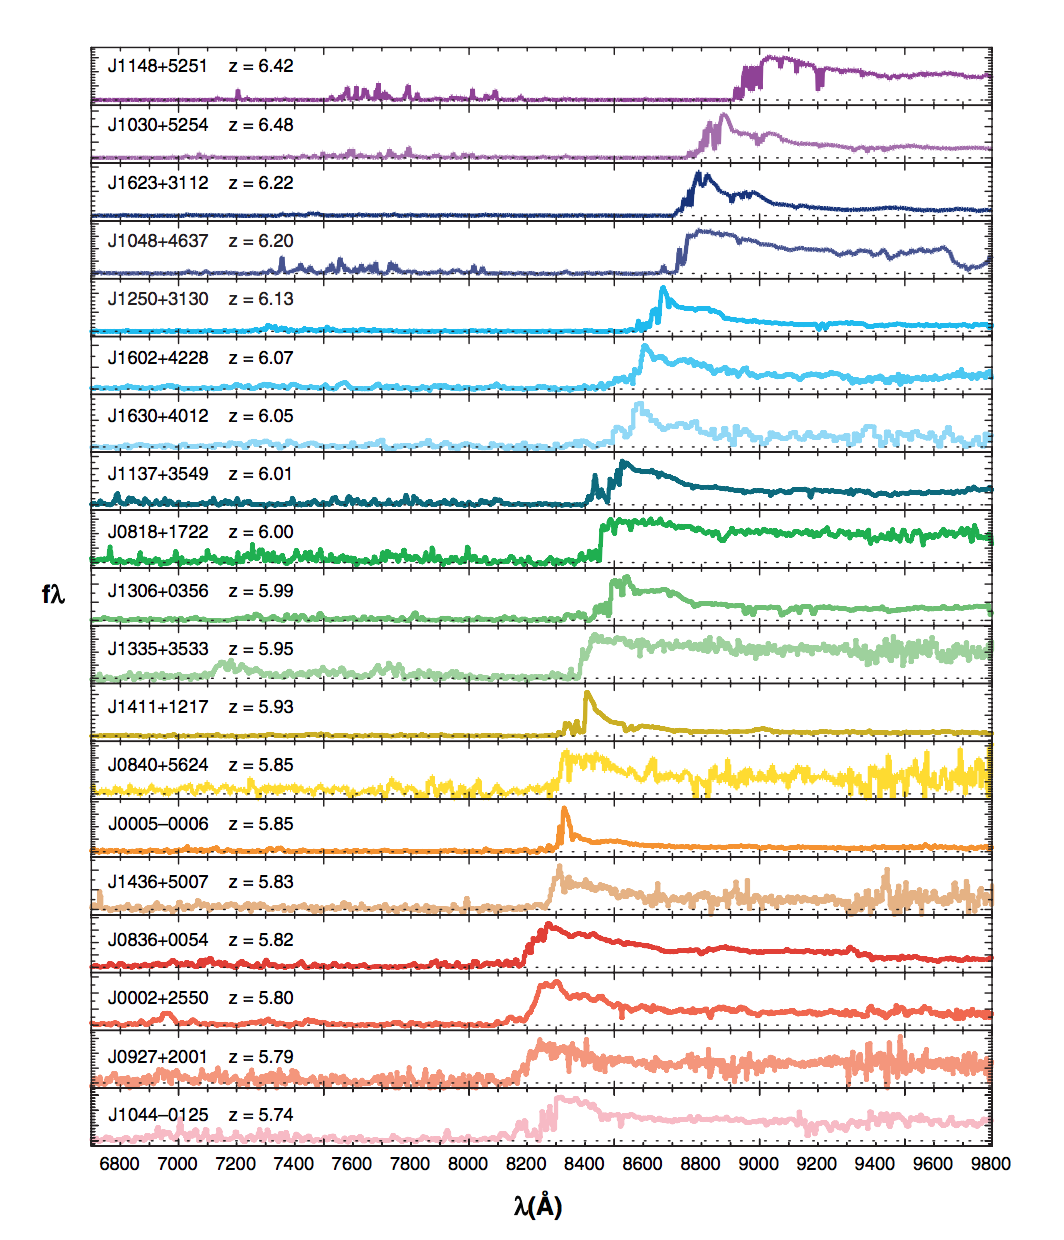
\includegraphics[width=0.8\textwidth]{chapters/eor_intro/figures/FanSpectra.png}
 \caption[The Ly$\alpha$ spectra of 19 high-redshift quasars.]{The Ly$\alpha$ spectra of 19 high-redshift quasars, as reported by \cite{Fan.06.2}. The effective optical depth towards each quasar increases with redshift, suggesting an evolution in the neutral fraction of the IGM. This figure was taken from \cite{Fan.06.review}.}
 \label{fig:eor_intro_qso}
 \end{figure}

Spectroscopic observations of high-redshift sources are relatively difficult to perform, and require large amounts of integration time. However, the distinctive Ly$\alpha$ limit in the spectra shown in Figure~\ref{fig:eor_intro_qso} is a distinctive property of high-redshift quasars. As an alternative, astronomers have developed a photometric method that is cheaper and easier to perform, called the ``Ly$\alpha$ dropout" technique. In this scheme, a survey will use an appropriate set of filters to probe a given redshift (imagine rectangles overlaid on the spectra in Figure~\ref{fig:eor_intro_qso}). If an excess is seen towards one galaxy in one filter, and very little signal is seen in the next-bluest filter, that galaxy may be considered a candidate high-$z$ quasar. With some modelling, the luminosity function of  Ly$\alpha$ dropout galaxies can be used to measure the mass distribution of galaxies as a function of redshift \citep[e.g.][]{Bouwens.15, Bouwens.16}. Using these luminosity functions and comparing to star formation rate models and measurements, \cite{Robertson.15} argue that current measurements are consistent with quasars playing a relatively minor role in reionization, with the bulk of ionizing photons arising form ``normal" galaxies rather than black hole accretion discs. However, this claim is moderately dependent upon uncertain model parameters, such as the escape fraction of ionizing photons from their local halo \citep{Robertson.13} and the star formation history at high redshifts. The latter is beginning to be answered as more high-redshift gamma-ray bursts are detected and characterized \citep{Wang.09, Robertson.12, Wang.15}.
%\footnote{In work unrelated to the bulk of this thesis, I presented observations of gamma-ray burst hosts suggesting that gamma-ray bursts were unbiased tracers of star formation rate -- a crucial component for using gamma-ray bursts to inform our understanding of the EoR \citep{Kohn.15}.}.

At the time of writing, photometric and spectroscopic observations of high-$z$ quasars suggest that the IGM had a neutral fraction $>10^{-4}$ at $z\sim 6$, indicating that the EoR ended around 1 Gyr after the Big Bang \citep{Barnett.17}. \cite{Fan.06.2} reported a direction dependence on their measurements, suggesting that reionization was patchy, rather than homogeneous.

\subsection{Observations of the CMB}
% CMB tau, kSZ
CMB photons will Thomson-scatter off-of free electrons in their path, suppressing the observed signal in a given direction. This suppression is described by an optical depth,

\begin{equation}
\tau_{\rm cmb} \propto \int^{z_{\rm recomb}}_0 x_i(z) a(z) \frac{{\rm d}l}{{\rm d}z}{\rm d}z,
\label{eq:eor_intro_tau_cmb}
\end{equation}
where $x_i(z)$ is the average ionized fraction at redshift $z$, $z_{\rm recomb}\approx1100$ is the redshift of recombination (and last scattering), $a(z) = (1+z)^{-1}$ and  ${\rm d}l/{\rm d}z$ is the cosmological line-element to redshift $z$. The optical depth to the CMB will suppress the observed primary anisotropies\footnote{The CMB is most-usefully described in harmonic $C_{\ell}$-space. Primary anisotropies, due to damped acoustic oscillations in the early hot plasma \citep{Silk.68}, are strongest at multipoles $\ell\lesssim3000$ -- equivalent to spatial scales $\theta \gtrsim 0.1^{\circ}$.} by a factor of $e^{-\tau_{\rm cmb}}$.

The dependence on $x_i(z)$ is crucial to our current understanding of the EoR; the largest contribution to the value of $\tau_{\rm cmb}$ will come from the large injection of electrons into the IGM during the EoR. Its measurement is not without complications: the suppression effect is degenerate with the overall amplitude of the CMB power spectrum, and it is an integrated quantity. 

The first complication can be addressed by performing polarized observations of the CMB, which breaks the degeneracy. A CMB photon that scatters off of an electron within a quadrupolar anisotropy will become linearly polarized, boosting polarized power at $\ell\sim2\sqrt{\tau_{\rm cmb}}$ \citep{Zaldarriaga.97.pol}. The WMAP satellite was the first telescope capable of making all-sky measurements of the CMB polarization, and detected an such an excess in polarized power, as shown in Figure~\ref{fig:eor_intro_spergel_tau} \citep{Kogut.03, Spergel.03}.

\begin{figure}
\centering
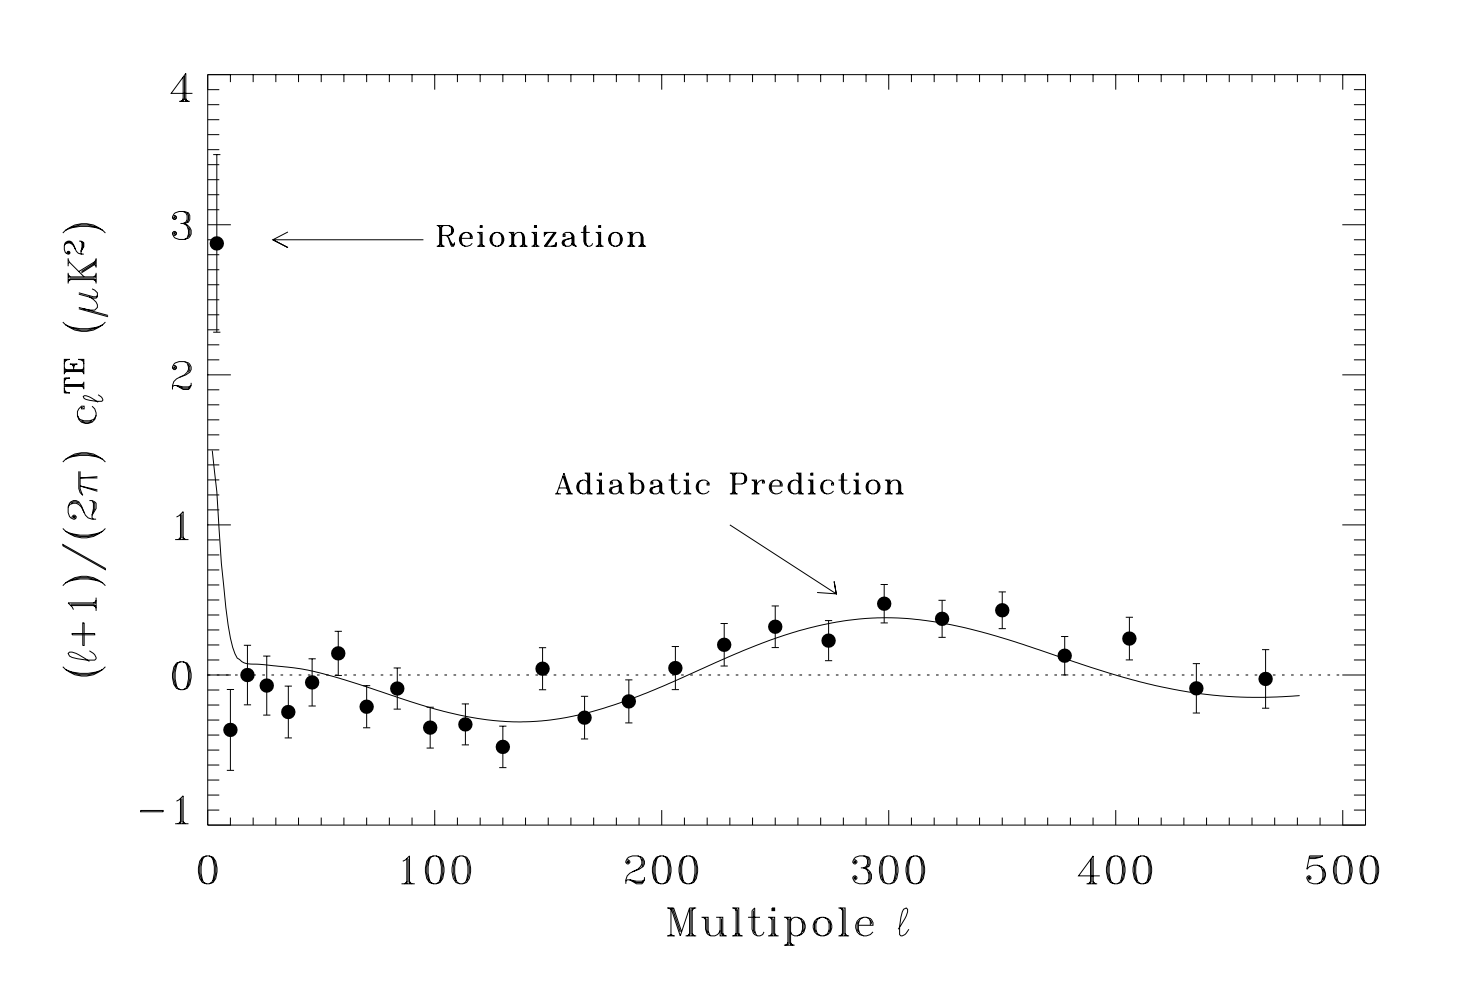
\includegraphics[width=0.8\textwidth]{chapters/eor_intro/figures/spergel_tau.png}
\caption[The $TE$ cross-power spectrum from WMAP.]{The Temperature-Linear Polarization ($TE$) cross-power spectrum from WMAP. The power was consistent with collisionless models save for an excess at large scales, consistent with large amounts of Thomson scattering of CMB photons during the EoR. Figure taken from \cite{Spergel.03}.}
\label{fig:eor_intro_spergel_tau}
\end{figure}

Such a measurement is able to recover a value of $tau_{\rm cmb}$, but due to its integral nature does not provide an ionization history. Values of $x_i(z)$ are therefore extremely model-dependent; typically extracted by assuming ``instantaneous reionization" in which $x_i(z)$ transitions from 0 to 1 quickly and smoothly. These models are often described using the tanh form:

\begin{equation}
x_i(z) \propto 1+\tanh\left(\frac{z - z_{\rm re}}{\Delta z}\right),
\end{equation}
where $z_{\rm re}$ is the redshift of instantaneous reionization, but is more usefully thought of as the redshift at which $x_i \approx x_{HI} \approx 0.5$. $\Delta z$ is the duration of reionization. Using such models, \cite{Planck.16.reionization} reported limits of  $7.8 < z_{\rm re} < 8.8$ and $\Delta z < 2.8$. They also reported that all of their modelling suggested that $x_i(z\gtrsim10)<0.1$.

The CMB provides us with more than one probe of reionization. \cite{Zeldovich.69} and \cite{Sunyaev.70} showed that CMB photons that scattered off of free electrons would introduce secondary anisotropies to the CMB (i.e. additional features in the $C_{\ell}$ spectrum). The Sunyaev-Zeldovich (SZ) effect is divided in to two categories: the thermal effect (tSZ) and the kinetic effect (kSZ). The tSZ occurs when CMB photons scatter off of electrons with high energies ($\sim 10$\,keV) due to their temperature; such high temperatures can only occur in high-mass galaxy clusters, and hence at redshifts lower than the EoR. 

The kSZ is of relevance to EoR studies. CMB photons scattering off of clouds of electrons in coherent velocity flows can be Doppler-shifted, which will redshift or blueshift (depending on the sign of the line-of-sight velocity) spectral observations of the CMB. Of course, clouds of electrons exist in relatively low-redshift galaxy clusters, and it was their contribution to the kSZ that was first detected \citep{Hand.12}. However, detection of the EoR contribution to the signal would be a powerful probe of dynamics on cosmological scales in the early Universe. The distortion induced by the kSZ on the CMB is given by

\begin{equation}
\frac{\delta T}{T_{\rm CMB}}(\hat{s}) = \frac{\sigma_T}{c} \int_0^{z_{\rm recomb}} n_e(z)e^{-\tau(z)} \hat{s}\cdot\vec{q} \frac{{\rm d}s}{{\rm d}z}{\rm d}z,
\label{eq:eor_intro_ksz}
\end{equation}
where $\sigma_T$ is the Thomson Cross Section, $n_e(z)$ is the average number density of electrons at redshift $z$, $\tau(z)$ is the optical depth to redshift $z$, and d$s$/d$z$ is the cosmological line element to redshift $z$ along direction $\hat{s}$. We can model inhomogeneities in the ionization and baryon fraction as vector field
\begin{equation}
\vec{q}(\hat{s}) = (1+\delta_x)(1+\delta_b)\vec{v}(\hat{s}),
\end{equation}
where $1+\delta_x = x_i/\left\langle x_i \right\rangle$, $1+\delta_b= \rho_b/\left\langle \rho_b \right\rangle$ and $\vec{v}$ is the free electron bulk flow.

This is an optical depth effect much like the optical depth of the CMB in Equation~\ref{eq:eor_intro_tau_cmb}. However, it has important distinctive features: it is a direction dependent, probing the velocity of electron bulk flows along the line of sight, rather than the average ionization history, and it can create excesses and decrements in power, depending on the sign of the velocity component.

Detection of the kSZ is difficult, as the secondary anisotropies it causes in brightness temperature are a few percent of tSZ. Compared to the primary anisotropies, the tSZ is roughly 10 times weaker in $\mathcal{D}_{\ell}=(\ell+1)\ell C_{\ell}/2\pi^2$, and the kSZ is roughly 100 times weaker.
\cite{George.15} reported a detection of the kSZ at $\ell\approx3000$ (where the primary anisotropies and the Cosmic Infrared Background, a CMB contaminant at small scales, are both close to their minimum values), using a suite of cosmological and spectral models to remove CMB foregrounds, the primary anisotropies and the tSZ \citep[e.g.][]{Shaw.10}. Again, measurements from the CMB are integrated quantities, so their constraints on reionization are model dependent. Using a symmetric model of reionization history \citep{Zahn.12}, they set the constraint that $\Delta z < 5.4$, with their likelihood peaking around $\Delta z = 1.3$. Using similar techniques with shallower data from the same telescope, \cite{Zahn.12} set consistent limits that $\Delta z \geq 2$, and also that reionization ended at $z>5.8$.

Wide-field measurements of the kSZ would be rewarding, but the foregrounds of the Galaxy, CIB, CMB and tSZ represent contemporary challenges for direct-imaging experiments. However, one could hope to use correlations of the velocity field the kSZ sources, and the density field associated with it, to decorrelate the foregrounds and estimate the underlying fields \citep[e.g.][]{Cooray.04, Alvarez.16}. The mathematical formalism for such a technique is laid-out in Chapter~\ref{chapter:ksz_21cm}.

\section{Direct measurements of {\sc hi}}
\label{sec:eor_intro_hi}

To borrow a line from \cite{DannyThesis}, the Dark Ages were not dark. Our Universe is dynamic and energetic, and particles constantly seek a lower energy state.

Throughout the Dark Ages and the EoR, {\sc hi} was shining, weakly, at radio wavelengths. The {\sc hi} atom is capable of a hyperfine transition between its ${}_{1}s_{1}$ and ${}_{0}s_{1}$ energy levels. The electron spin can spontaneously change from parallel to the proton spin to antiparallel, emitting a photon of frequency $\nu_{21\,cm}\approx1420.4$\,MHz; a rest-wavelength of roughly 21\,cm. The emission coefficient of this transition is $\sim 2.9\times10^{-15}\,s^{-1}$, corresponding to a half-life of approximately 11 million years per atom. This is both the strength and the weakness of observing {\sc hi}. According to Fermi's Golden Rule, the probability of emission is equal to that of absorption; a small transition rate leads to a relatively dim signal, but 21\,cm photons are extremely unlikely to be observed between their emission and observation. This allows the 21\,cm signal to be tomographically mapped -- a sharp excess at the relevant frequency indicates a redshift -- and constructed into a 3D cube in space and time.

Observations of {\sc hi} during the Dark Ages and the EoR would directly constrain the ionization history of the Universe, allowing us to probe the evolution of the density field at high redshifts, the properties of the first stars, galaxies and black holes, and map the structure of the IGM as it evolves as a function of redshift. It would also represent the furthest baryons ever detected, and the largest volume of the Universe ever surveyed. This Section reviews the nature of the 21\,cm line during the EoR, and two parallel endeavours to detect it, using the monopolar signal (i.e. power averaged over the sky), and the anisotropic signal (power as a function of spatial scale).

\subsection{The 21cm transition}

As noted above, the probability of a single {\sc hi} atom undergoing the 21\,cm transition is exceedingly small. However, during the Dark Ages and the EoR, {\sc hi} was ubiquitous, and such transitions would be occurring constantly.
The relative occupancy of the hyperfine state in {\sc hi} is given by

\begin{equation}
\frac{N_1}{N_0} = \frac{g_1}{g_0} e^{-h\nu_{\rm 21cm}/k_B T_S},
\end{equation}
where $g_1$ and $g_0$ refer to the triplet and singlet states of the atom and are equal to 3 and 1, respectively. This Equation defines the spin temperature $T_S$, an analog of molecular excitation temperature for {\sc hi}. By solving the radiative transfer equation for this system in the Rayleigh-Jeans limit \citep[e.g.][]{MooreThesis}, we can write the brightness temperature of the emission as:

\begin{equation}
T(z) = T_S \tau_{\nu}(z) + T_{\rm bg}(1-\tau_nu(z)),
\label{eq:eor_intro_brightness_temp}
\end{equation}
where the optical depth of {\sc hi}, $\tau_{\nu}$, is assumed to be small, and the temperature of the background radiation $T_{\rm bg}$ is, for EoR observations, the temperature of the CMB at redshift $z$. \cite{Furlanetto.06} showed that the optical depth can be expressed in terms of cosmologically-interesting quantities, assuming the IGM is diffuse:

\begin{equation}
\tau_{\nu} \approx 9.2\times10^{-3} (1+\delta_b)(1+z)^{3/2}\frac{x_{HI}}{T_S}\frac{H(z)}{1+z}\frac{{\rm d}v_{\parallel}}{{\rm d}r_{\parallel}},
\end{equation}
where d$v_{\parallel}$/d$r_{\parallel}$ is the component of the peculiar velocity of the {\sc hi} cloud per unit depth along the line-of-sight, with respect to the Hubble expansion given by $H(z)/1+z$. The prefactor of $9.2\times10^{-3}$ justifies the assumption of small $\tau_{\nu}$ made above. Comparison to the optical depth for the Ly$\alpha$ line in Section~\ref{sec:eor_intro_current} emphasizes that {\sc hi} observations refer an opposite regime of EoR probes.

Combining the above equations, we can define the brightness contrast between redshifted {\sc hi} emission and the CMB,

\begin{equation}
\delta T \approx 9{\rm mK} \times x_{HI} (1+\delta_b)(1+z)^{1/2} \left( 1 - \frac{T_{\rm CMB}(z)}{T_S} \right)
\left( \frac{H(z)/(1+z)}{{\rm d}v_{\parallel}/{\rm d}r_{\parallel}} \right).
\label{eq:eor_intro_dT_reionization}
\end{equation}

Note that $\delta T$ can saturate if $T_S \gg T_{\rm CMB}$, and can become arbitrarily negative if $T_S \ll T_{\rm CMB}$. The observed emission is `backlit' by the CMB -- it's observability hinges on its relationship to $T_{\rm CMB}$.
Also note that the characteristic brightness temperature in Equation~\ref{eq:eor_intro_dT_reionization} is of order mK. By the time it is observed, the 21\,cm emission from the EoR has redshifted into meter wavelengths. At these wavelengths, Galactic synchrotron dominates the sky with brightness temperatures $\sim 10^3$\,K (see Chapter~\ref{chapter:astro_rad}; \citealt{McQuinn.07}). Foreground removal or avoidance remains the primary challenge for all EoR experiments, and will be discussed extensively throughout this thesis. I believe that the promises of 21\,cm tomography, outlined below, make the challenge worth pursuing. For a comprehensive reviews of the theory behind high-redshift 21\,cm tomography, see \cite{Madau.97}, \cite{Furlanetto.06} and \cite{Pritchard.10}. 

It is important to mention here, and will be re-iterated, that the 21\,cm photons generated through the hyperfine transition are highly unpolarized. Primordial magnetic fields could induce circular polarization via Zeeman splitting, but such an effect would be 3 to 4 orders of magnitude smaller than the already faint total intensity signal itself \citep[e.g.][also see Chapter~\ref{chapter:astro_rad}]{Babich.05}.

% spectral structure?

% why is it interesting (near term) - Liu Tau constraints, Kittiswitt maps (topology of EoR = cool), Kern emulators -- sensitivity to astrophysics & cosmology

\subsection{Global signal}
% WF coupling

The sky-averaged 21\,cm signal, sometimes called ``global signal", is a direct measurement of the spin temperature as a function of redshift. Equation~\ref{eq:eor_intro_brightness_temp} can be approximated as \citep{Field.56}:

\begin{equation}
T_S^{-1} = \frac{T_{\rm CMB}^{-1} + x_cT_K^{-1} + x_{\alpha}T_c^{-1} }{1 + x_c + x_{\alpha}}
\end{equation}
where $x_c$ and $x_{\alpha}$ are coupling coefficients for collisions and UV scattering, respectively, $T_K$ is the kinetic temperature of the gas, and $T_c$ is the effective temperature of the UV radiation field. The magnitude and sign of $T_S$ with respect to $T_{\rm CMB}$ is therefore proportional to each coupling constant.

At high redshifts, \cite{Wouthuysen.52} and \cite{Field.59} showed that there was good reason to expect that $T_c \rightarrow T_K$, such that $T_S$ decouples from $T_{\rm CMB}$. The effect -- now known as the Wouthuysen-Field Effect -- relies on Ly$\alpha$ radiation from early luminous sources exciting {\sc hi} in the ${}_1s$ states into the ${}_2p$ states. The atoms can then decay to the  ${}_1s_1$ state via allowed transitions, overpopulating that hyperfine energy level. This couples the {\sc hi} to the UV radiation field; the strength of the coupling depends on the spectral shape of the Ly$\alpha$ line. Increasing the coupling to UV scattering would make $T_S$ large and negative.

A fiducial reionization history is shown in Figure~\ref{fig:eor_global_signal_sketch} \citep{Mirocha.12}, with important turning points and zero-crossings highlighted. Working forwards through history, collisional coupling is relatively large in the Dark Ages, and couples $T_S$ to a low $T_K$, creating an absorption trough. The Universe continues to expand, baryon density drops, and $T_S$ and $T_K$ decouple; $T_S$ tends towards zero as it grows closer to $T_{\rm CMB}$.
As the first stars ignite, marking the end of the Dark Ages, their UV emission couples to the spin temperature via the Wouthuysen-Field Effect, creating a sharp absorption feature. As more massive structures form, X-rays begin to dominate the ionizing radiation field, increasing $T_K > T_{\rm CMB}$ such that the 21\,cm signal is seen in emission for the rest of the EoR. The 21\,cm spin temperature goes to zero, as it must, at the end of the EoR \citep[e.g.][]{Pritchard.10, Rao.17}. 

\begin{figure}
\centering
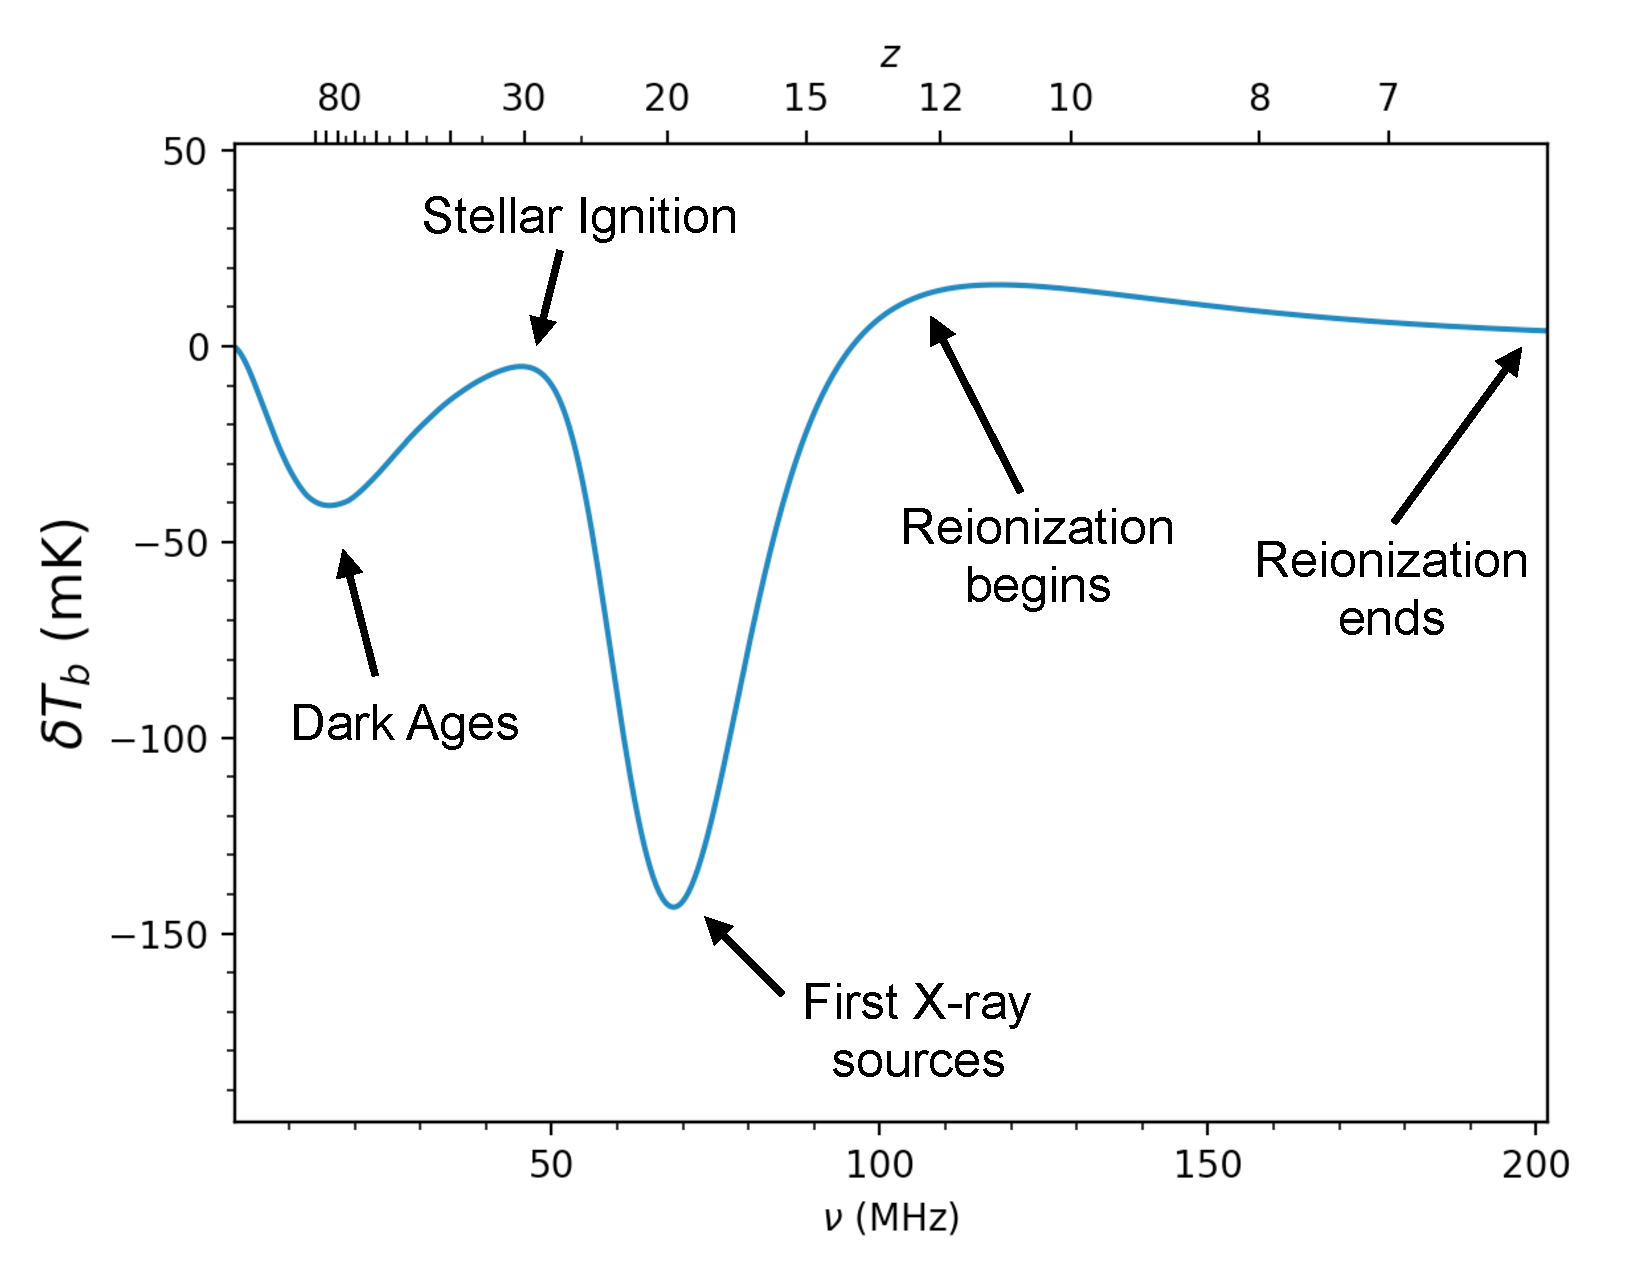
\includegraphics[width=0.8\textwidth]{chapters/eor_intro/figures/ares_sketch.pdf}
\caption[The history of the EoR global signal.]{The history of the EoR global signal, with important turning-points indicated. This figure was produced using the fiducial model of \cite{Mirocha.12}.}
\label{fig:eor_global_signal_sketch}
\end{figure}

Given the history described above, detection of the global signal would provide key information about the thermal history of the IGM as a function of redshift, and about the high-energy emission spectra of early stars and galaxies. Historically, observational efforts to detect the global signal have been ``single dish'' experiments, where a single receiving element is characterized to high precision, and then operated in an effort to detect the EoR signal as a function of frequency (and thus redshift). Such experiments typically seek to characterize the location and depth of the turning points, with the advent of X-ray sources giving the highest potential signal-to-noise. Experiments such as the Experiment to Detect the Global EoR Step (EDGES, \citealt{Bowman.10}), Sonda Cosmol\'{o}gica de las Islas para la Detecc\'{i}on de Hidr\'{o}geno Neutro (SCI-HI, \citealt{Voytek.14}), and the Cosmic Twilight Polarimeter (CPT, \citealt{Nhan.16}), have been proposed or constructed seeking to measure the global signal from the Dark Ages or the EoR, through a deep understanding of the properties of the instruments.

In all cases, the instruments consist of a single element, and much of the observational effort contributes toward a thorough understanding of systematic uncertainties of the instrument. Given that the signal is thought to be 4--5 orders of magnitude fainter than the foregrounds, an exquisite understanding of the correlated noise in these instruments is of the utmost importance. At the time of writing, the most mature global experiment is EDGES, an extremely well-characterized radio spectrometer. By subtracting a precise model of the foreground spectrum (\citealt{Rogers.08}, improved upon by \citealt{Mozden.17}), \cite{Bowman.10} were able to set a lower limit on the length of the reionization tail (and hence of the EoR itself) of  $\Delta z \geq 0.06$, ruling-out instantaneous reionization.

Excitingly, as this Chapter was being written, the EDGES team announced a detection of the X-ray heating turning point at 78\,MHz \citep{Bowman.18}. Their detected absorption trough was so deep, however, that it exceeds physical models for the (negative) magnitude of $T_S$. \cite{Bowman.18} and \cite{Barkana.18} suggested that the excess depth could be accounted for by additional collisions with dark matter. \cite{Ewall-Wice.18.edges} have shown that the excess could also be accounted for by an additional radio background from early black holes formed form Pop{\sc iii} stars. Confirmation from other global signal experiments will be required before the \cite{Bowman.18} result can be fully trusted, but it leaves open the possibility of {\sc hi} global signal experiments probing exotic particle physics, as well as astrophysics and cosmology.

\subsection{Anisotropic signal}

While the global signal may be computed by measuring the average brightness temperature at a given frequency, a richer astrophysical story can be told by measuring the anisotropies in the spin temperature at each redshift. Similarly to the CMB, these anisotropies can be represented through a 2-point correlation function; a power spectrum in Fourier space. Unlike the CMB, of course, this power spectrum  can be measured at each frequency observed, allowing us to construct a history of {\sc hi} emission on different spatial scales. 

Inspection of Equation~\ref{eq:eor_intro_dT_reionization} shows that the fluctuations will trace the underlying baryonic density field, but with a complicated bias depending upon the ionization fraction, peculiar velocities and importantly the nature of the ionizing sources, their clustering and their UV and X-ray spectra. This convolution of astrophysical and cosmological dependencies means that the redshift dependence of a given Fourier mode will give clues about the ionization history. Maxima represent high contrasts in the brightness temperature field, suggesting middle stages of the EoR. However, the bulk of information contained in power spectra will require models to extract. This requirement is not as onerous as it might sound, thanks to decades of theoretical work (an exhaustive list is impossible, but the literature reviews of \citealt{Grieg.17} and \citealt{Kern.17} provide useful starting points). 

For example, Figure~\ref{fig:eor_intro_liu_history} shows the enormous improvement in modelling the ionization history, given high signal-to-noise measurements of the 21\,cm power spectrum. Including {\sc hi} data leads to precise constraints on $x_{HI}(z)$ -- but the constrains may be inaccurate in their timing of the EoR without including CMB polarization measurements. 

\begin{figure}
\centering
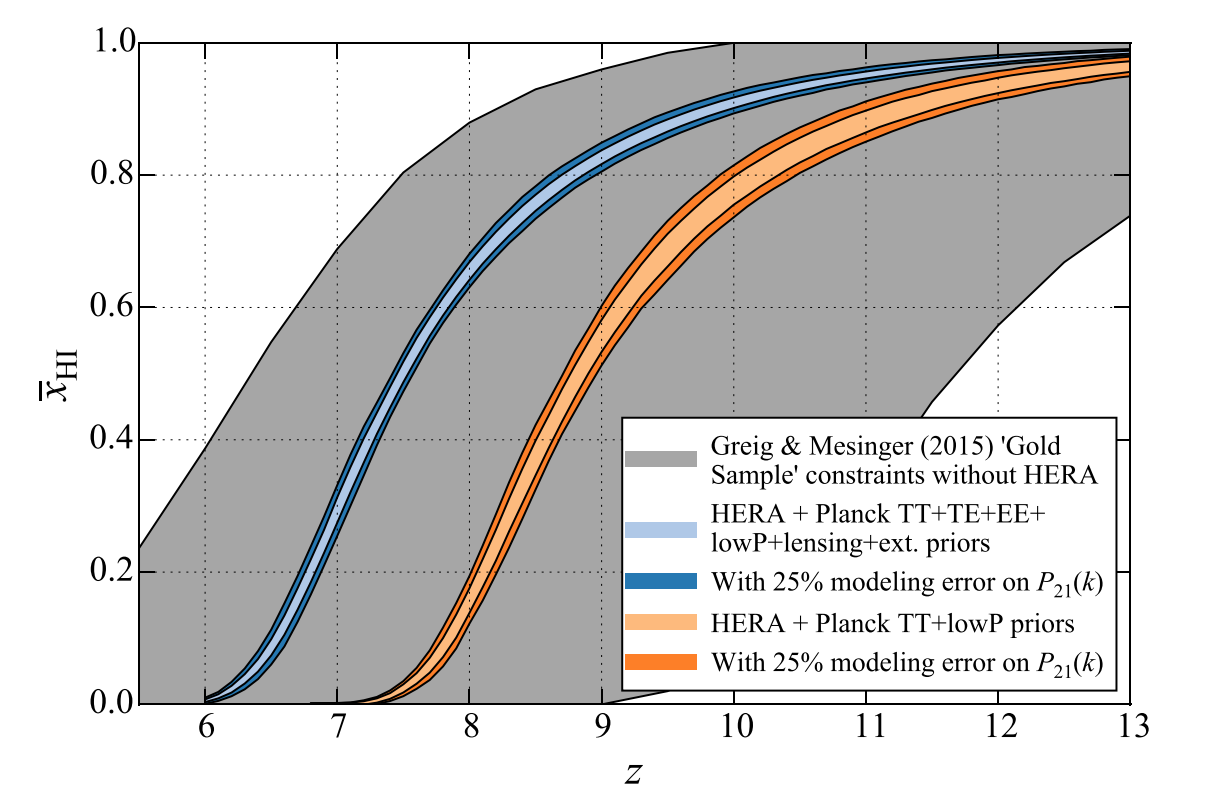
\includegraphics[width=0.7\textwidth]{chapters/eor_intro/figures/Liu_history.png}
\caption[Forecasts for constraints on the ionization history, given high signal-to-noise measurements of the {\sc hi} power spectrum at each redshift from HERA.]{Forecasts for constraints on the ionization history, given high signal-to-noise measurements of the {\sc hi} power spectrum at each redshift from HERA. The grey band shows constraints on the ionization history without measurements of {\sc hi}, while the blue and orange curves include power spectrum measurements in their modelling. Without CMB polarization measurements, an shift in the timing of reionization can occur. Figure taken from \cite{Liu.16}.}
\label{fig:eor_intro_liu_history}
\end{figure}

As discussed in Section~\ref{sec:eor_intro_current}, parametrizing the optical depth to the CMB can grant a model-dependent measurement of the ionization history, but one must rely on models in which reionization occurs very quickly. Curves such as those shown in Figure~\ref{fig:eor_intro_liu_history} would eliminate the need for such models by providing a measurement of the ionization history. This in turn can break degeneracies in other measurements from the CMB. For example, \cite{Liu.16.tau} showed that estimates of the sum of neutrino masses\footnote{Understanding the sum of the masses of the three flavors of neutrinos is a critical measurement in the realm of quantum chromodynamics. It is informed by the CMB, as neutrinos can suppress the formation small-scale anisotropies.} can be improved by $\sim10\%$ -- importantly, with likelihood contours perpendicular to other probes.

\cite{Kern.17} used machine-learning techniques to generate a suite of emulators for the {\sc hi} power spectrum. Given measurements of the power spectrum as a function of redshift, with realistic errors and foreground mitigation, their emulators would be able to constrain cosmological and astrophysical parameters for the EoR and the Dark Ages to relatively high precision. Their constraints on astrophysical parameters were tighter than cosmological ones due to the fact that the brightness contrast is a complicated proxy for the cosmic density field. To illustrate this complication, we show slices of simulation cubes in Figure~\ref{fig:eor_intro_plp_sim}, showing the baryon density field and the corresponding 21\,cm brightness temperature close the middle of the EoR. In the bottom panel, we show the evolution of the 21\,cm field along the line of sight, emphasizing that EoR measurements can provide a rich history of the IGM.

\begin{figure}
\centering
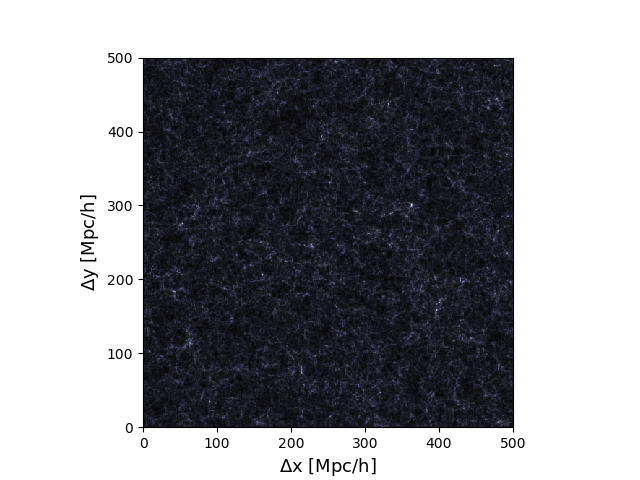
\includegraphics[width=0.5\textwidth]{chapters/eor_intro/figures/density.png}
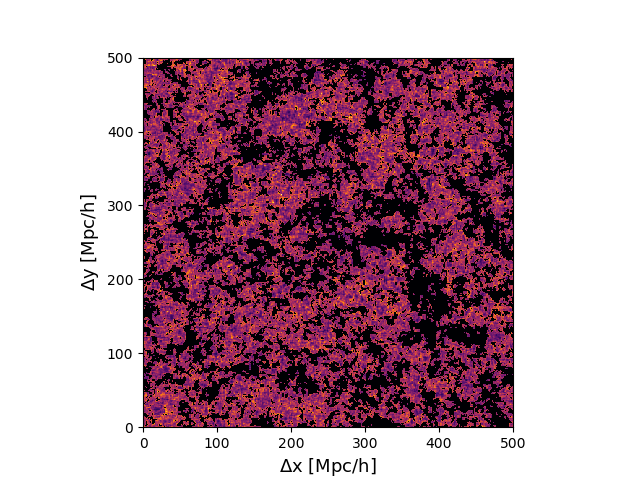
\includegraphics[width=0.5\textwidth]{chapters/eor_intro/figures/t21.png}
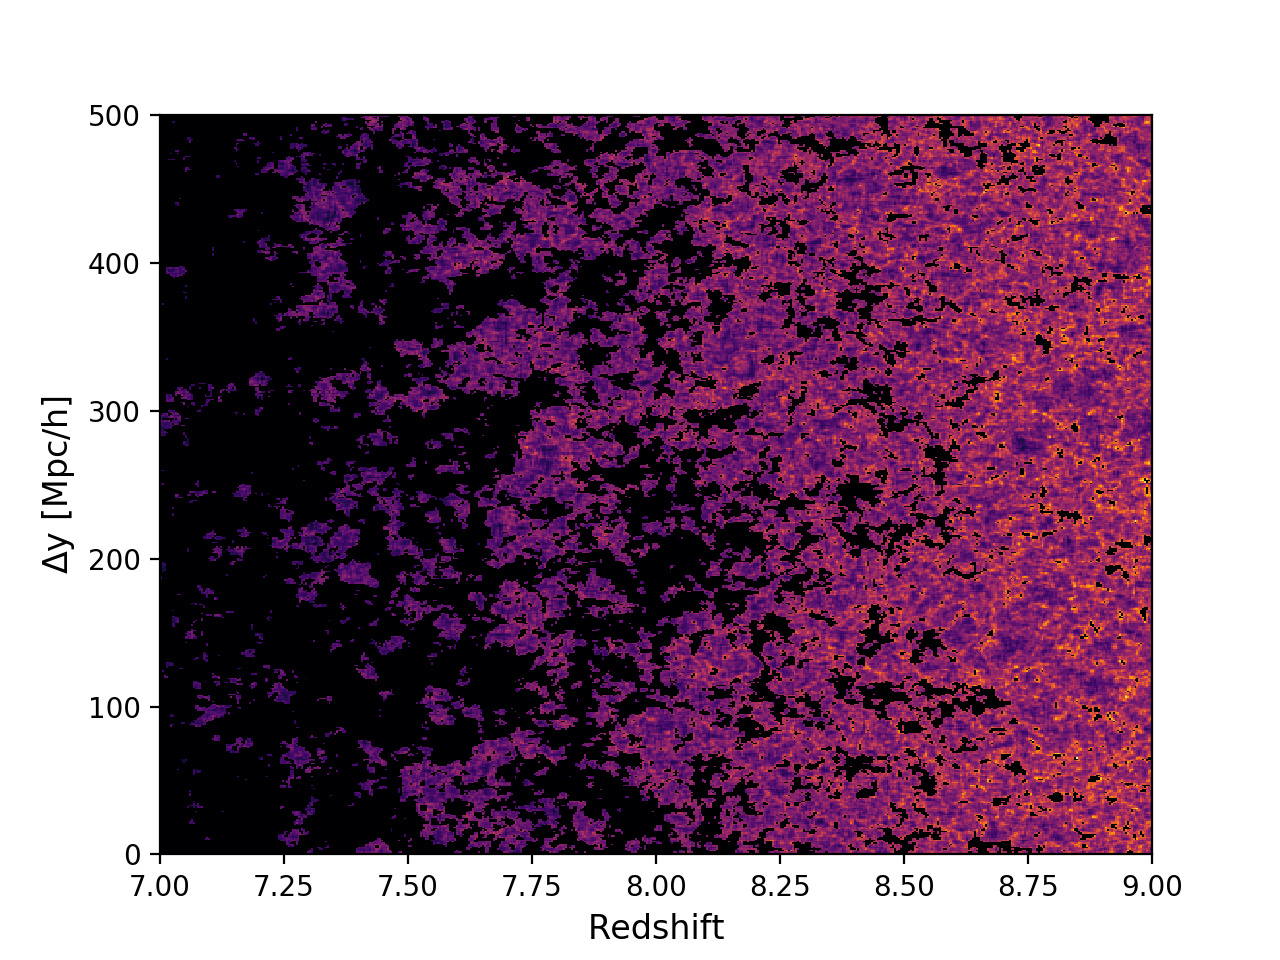
\includegraphics[width=0.5\textwidth]{chapters/eor_intro/figures/t21_z.png}
\caption[An example cosmological simulation of the EoR and the corresponding density field.]{An example cosmological simulation of the EoR. The upper panel is the baryon density field, and middle one is the corresponding 21\,cm brightness contrast, both at redshift $z\sim 8$. Both fields have been normalized for this illustration, the purpose of which is to show that there is not a simple mapping between the cosmological density field and the {\sc hi} observable. The bottom panel shows the 21\,cm brightness contrast as a function of redshift.}
\label{fig:eor_intro_plp_sim}
\end{figure}

Moving beyond statistical measurements to maps of the EoR\footnote{The reason for this order is due to the strength of the foregrounds, and strategies employed mitigate them. These will be explored at length in Chapter~\ref{chapter:eor_window_theory}.} opens a rich window for observational cosmology. Performing real-space tomography would allow us to construct cubes of the {\sc hi} field at different redshifts. Studying the shape and size of bubbles would provide us with a way to identify individual ionizing sources and interpret them. \cite{Robertson.15} showed that there are barely enough galaxies to account for the ionization of the Universe, suggesting that other sources such as quasars must play a role -- the signature of which would be detectable in tomographic cubes (Chapter~\ref{chapter:hera_ml}, shows an initial machine learning framework to perform this characterization). % more imaging things?

Radio interferometers (see Chapter~\ref{chapter:interferometry}), are excellent instruments for probing temperature anisotropies, and their measurements naturally translate into the Fourier space native to power spectrum measurements (see Chapters~\ref{chapter:instruments} and \ref{chapter:eor_window_theory}). Interferometers currently pursing detection of the EoR power spectrum include the Giant Meterwave Radio Telescope \citep[GMRT;][]{Paciga.13}, the Low Frequency Array \citep[LOFAR;][]{vanHaarlem.13}, the Murchinson Widefield Array \citep[MWA;][]{Tingay.13}, the Donald C. Backer Precision Array for Probing the Epoch of Reionization \citep[PAPER;][]{Parsons.10} and the Hydrogen Epoch of Reionization Array \citep{deBoer.17}.

Low-frequency radio interferometers such as those listed above have not yet reported results of sufficient depth to claim a detection of the EoR power spectrum. This is largely due to the major challenge faced by all EoR experiments -- extremely bright foregrounds. The intensity of the synchrotron radiation that dominates the low-frequency sky scales as a power law in frequency, so probing higher and higher redshifts becomes more and more difficult (see Chapter~\ref{chapter:astro_rad}). As we discuss in Chapter~\ref{chapter:eor_window_theory}, the chromatic response of an interferometer may provide a crucial lever arm for disentangling foreground and background radiation. The instrument itself also behaves as a foreground, as at such low frequencies, thermal noise in the electronics is a much larger fraction of the `observed' signal than redshifted 21\,cm emission.

\section{Current Limits and Future probes}
\label{sec:eor_intro_future}

Over the past decade, immense progress has been made to constrain the global history of the EoR. To review a few limits that have been discussed in this Chapter, limits from quasars and the kSZ have set the end of reionization $5.8 < z_{\rm end} < 6.0$. Measurements of the optical depth to the CMB have set model-dependent limits that put the middle of reionization at $7.8 < z_{\rm mid} < 8.8$. Combining kSZ measurements with the optical depth of the CMB has set an upper limit on the duration of the EoR, and measurements from EDGES have set a lower limit, such that $0.06 < \Delta z < 2.8$.

Current kSZ limits and low-significance detections, and measurements from quasars, are consistent with a patchy EoR -- bubbles opening to create an inhomogeneous spin temperature field. Figure~\ref{fig:eor_intro_pspec_limits} shows current limits on the EoR power spectrum from radio interferometers, as a function of redshift {\color{red} (Kolopanis et al., in prep.)}. The limits correspond to different spatial scales, but until some scale-dependence of the EoR power spectrum is detected, plotting them along side one another is valid. Integrations are becoming successively deeper, but there is a ways to go, as shown by a fiducial reionization power spectrum curve \citep{Mesinger.11}. Deeper integrations require more interferometric baselines and longer observing seasons, both of which require precision calibration and control of instrument systematics. New techniques for some of these challenges are presented in Part {\sc ii}.

\begin{figure}
\centering
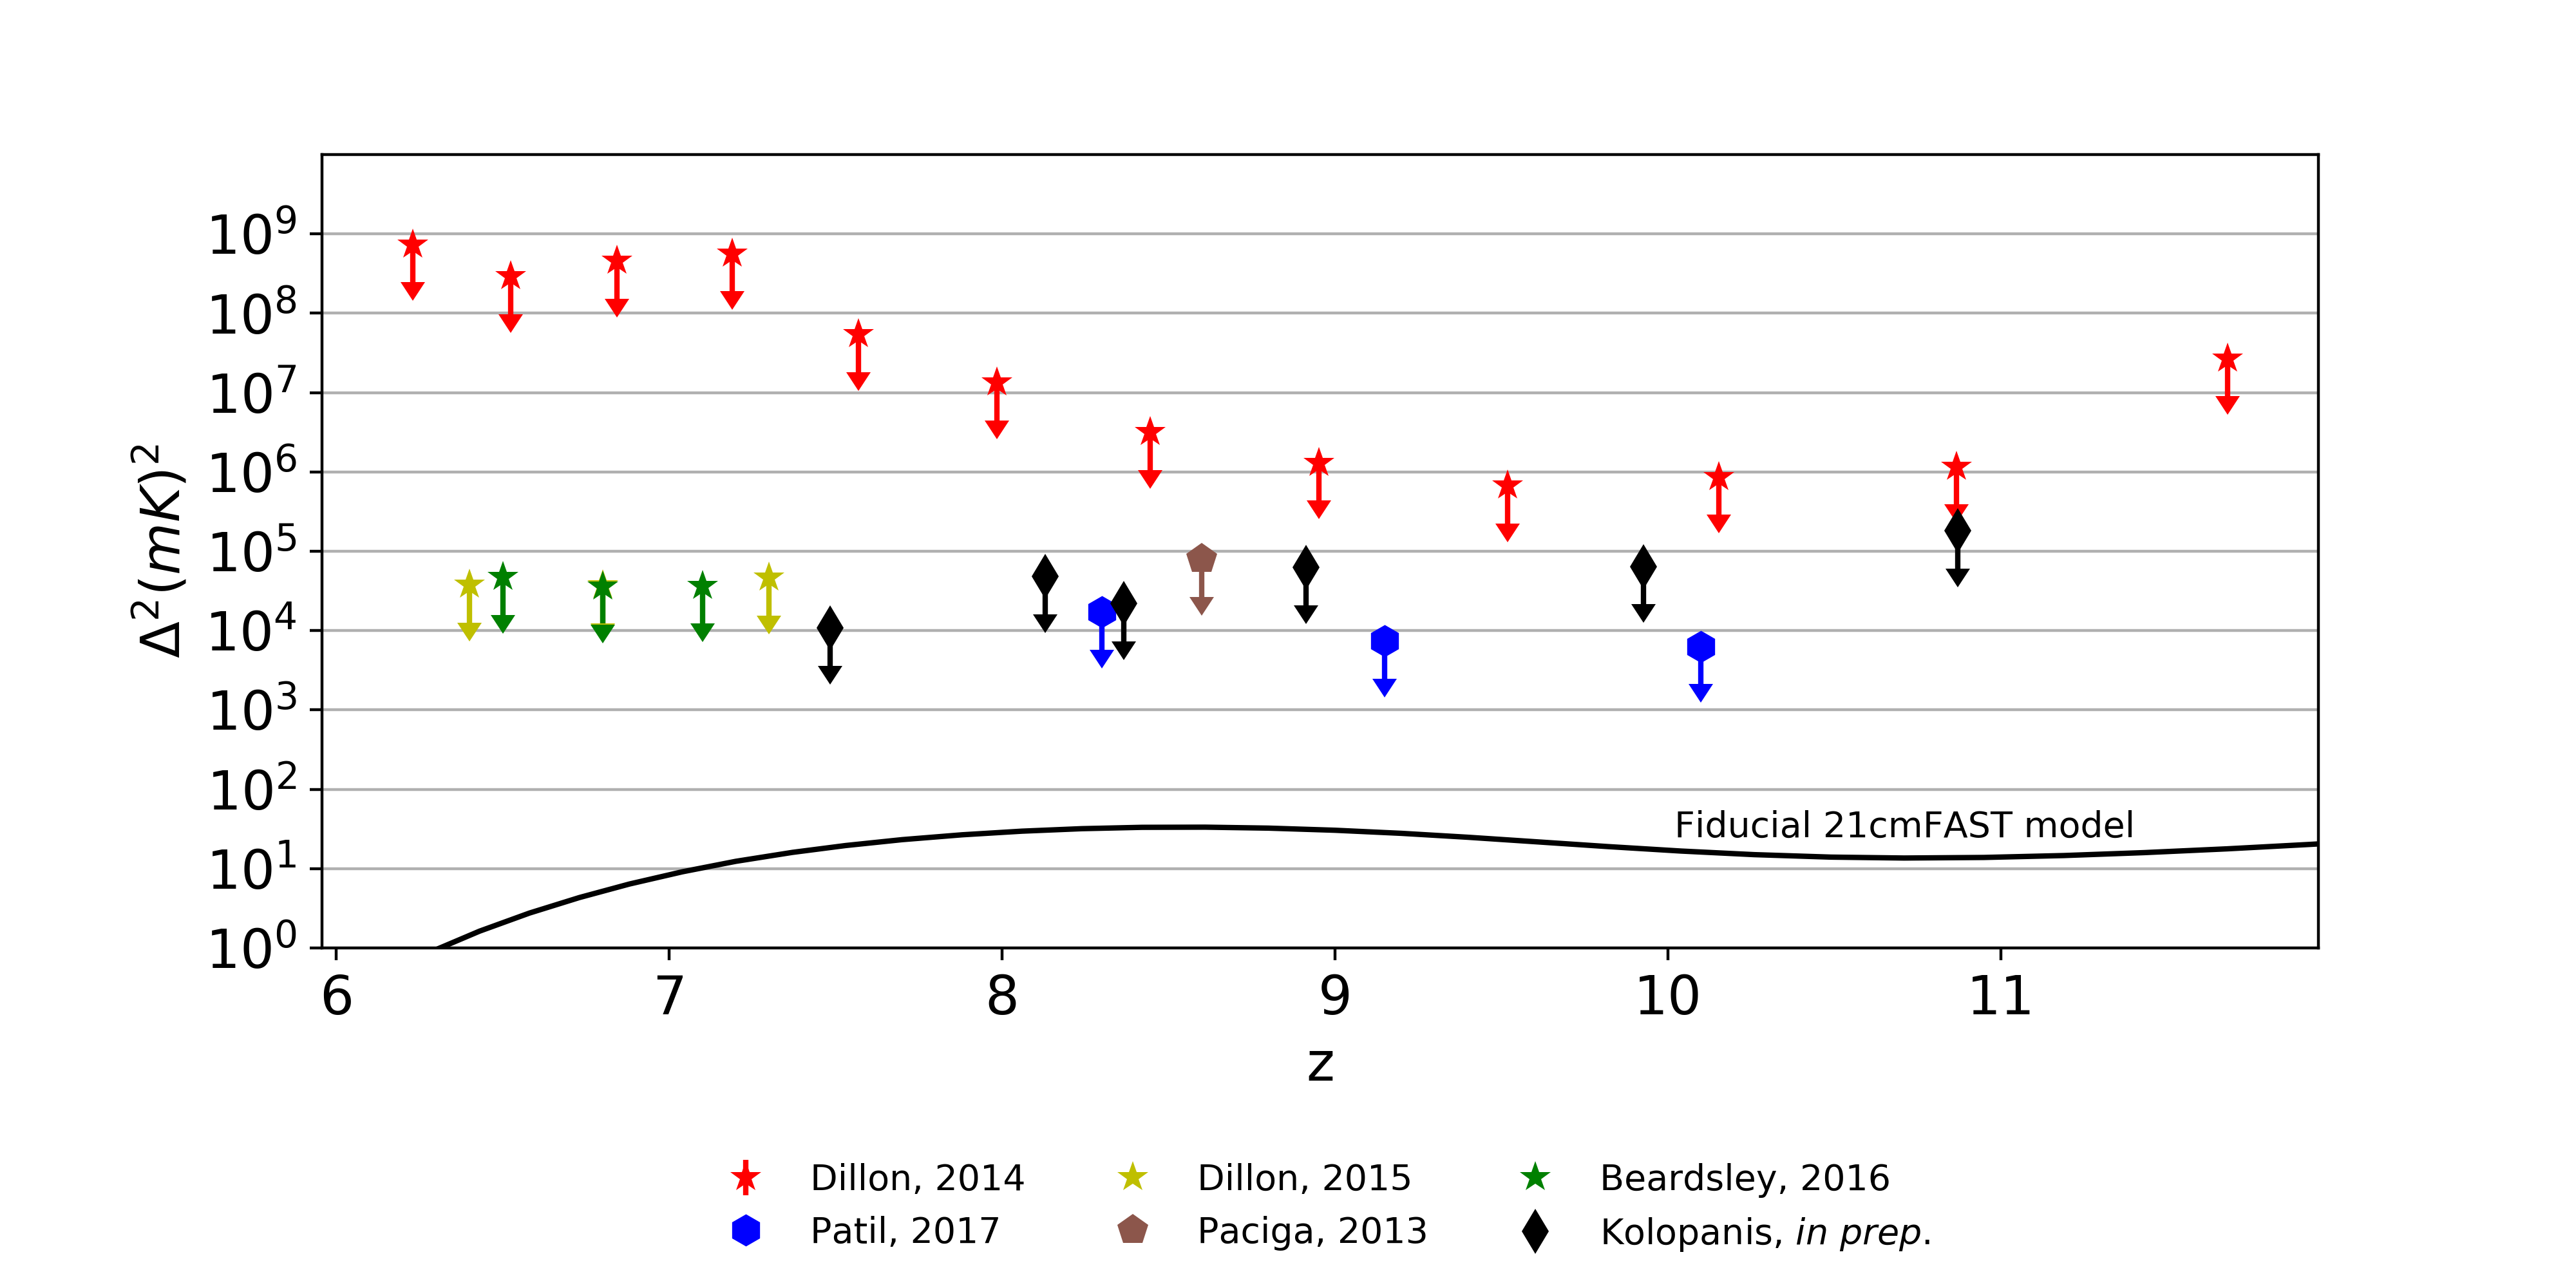
\includegraphics[width=0.8\textwidth]{chapters/eor_intro/figures/eor_lowest_limits.png}
\caption[Current limits on the EoR power spectrum, as a function of redshift.]{Current limits on the EoR power spectrum, as a function of redshift. Different symbol shapes correspond to different instruments, with stars \citep{Dillon.14, Dillon.15, Beardsley.16} indicating measurements from the MWA, blue hexagons \citep{Patil.17} from LOFAR, the brown pentagon from the GMRT \citep{Paciga.13} and the black diamonds from PAPER-64 {\color{red} (Kolopanis et al., in prep.)}. Figure taken from {\color{red} Kolopanis et al., in prep}. Plotted beneath all of the limits is a fiducial 21\,cm power spectrum \citep{Mesinger.11} -- there is still a factor of $\sim 10^3$ to integrate-down upon.}
\label{fig:eor_intro_pspec_limits}
\end{figure}

This Chapter has reviewed our current understanding of the EoR, and why it's observation would represent an enormous advancement for modern cosmology. The pursuit of realizing 21\,cm tomography is relatively mature, but other atomic transitions could contain similar promise. \cite{Silva.13} suggested that one could perform an intensity-mapping survey of Ly$\alpha$ emission. Such an experiment would involve several narrow-band filters to extract the high-redshift Ly$\alpha$ power spectrum at $z\sim7$, statistically probing the population of ionizing sources towards the end of the EoR, when Ly$\alpha$ is detectable. Narrow-band surveys for Ly$\alpha$ emission yielded a possible detection of Pop{\sc iii}-like stars at $z\sim 6.6$ \citep{Sobral.15}.

Carbon is easily ionized by diffuse starlight. The forbidden [C{\sc ii}] transition in ionized carbon could be used to perform tomography with advantages similar to {\sc hi}, as a probe of star formation history. At EoR redshifts, the emission line would redshift into an atmospheric window detectable in the Far Infra-red from Earth \citep[e.g.][]{Gong.12, Hunacek.16, Pentericci.16}. 
The polar nature of the CO molecule leads to a quantization of its energy states in integer multiples if its angular momentum, appearing as a `ladder' of emission lines that can be used for extremely precise redshift determination, and the relative intensity of which are determined by the temperature of the molecular cloud. Intensity mapping CO emission could provide a cosmic history of star forming giant molecular clouds \citep[e.g.][]{Righi.08,Lidz.11.CO}.
It is worth mentioning that all of these intensity mapping proposals suggest cross-correlation with 21\,cm tomographic measurements as a central science objective.

The James Webb Space Telescope is scheduled to launch between October 2018 and June 2019, and will be the most sensitive infra-red telescope ever constructed \citep{jwst}. It is predicted to be able to detect small mass halos ($\sim 10^5 M_{\odot}$) at $z\sim 10$ in its planned ultra-deep integrations \citep{Salvaterra.11, Zackrisson.11}. Its relatively small field of view will not allow for comprehensive surveys of the high-redshift Universe or the EoR, but correlating its measurements with 21\,cm maps would provide a probe of the dependence of high-redshift galaxies on their ionization environment \citep[e.g.][]{Beardsley.15}.

\section{This thesis}
\label{sec:eor_intro_this_thesis}
Everything in this work -- algorithmic development, mathematical theory, observations -- was carried-out in order to facilitate the detection of the EoR. While these efforts took many forms, they shared that singular motivation of moving the field forward, towards a detection of {\sc hi} anisotropies at cosmological distances. 

This thesis is divided into three parts. Part {\sc i} is devoted to introducing concepts used throughout this work and building a mathematical formalism around those concepts. 
Chapter~\ref{chapter:astro_rad} reviews astrophysical mechanisms for producing polarized and unpolarized radiation at low radio frequencies. 
Chapter~\ref{chapter:interferometry} builds a formalism around measuring low frequency radio waves with interferometers (and the challenges associated with accurately measuring polarized radiation), and Chapter~\ref{chapter:instruments} introduces the instruments used throughout this work.

In Part {\sc ii} I present the bulk of my efforts: building an understanding of the imprint of the polarized sky, and the instrument itself, in the Fourier space used to set limits on the EoR power spectrum. 
Chapter~\ref{chapter:eor_window_theory} reviews the current theory and major results of mapping low frequency interferometric measurements into Fourier space. 
Chapter~\ref{chapter:data_prep_and_proc} details several required quality assurance and compression steps that must be taken to clean and interact with the data. Building from clean data, Chapter~\ref{chapter:polcal} presents new algorithms developed to calibrate the measurements.
Chapter~\ref{chapter:ionosphere} discusses the impact of Earth's ionosphere on our measurements.
In Chapters~\ref{chapter:eor_window_paper32img}, \ref{chapter:eor_window_HERA} and \ref{chapter:eor_window_psa128} I present successively-deeper integrations on polarized foregrounds in successively-narrower regions of Fourier space.

Part {\sc iii} explores other uses of EoR measurements, beyond detection of the power spectrum. In Chapter~\ref{chapter:TAV}, I discuss the potential of using long time-averages of interferometric measurements to measure some component of the monopole moment of the sky. In Chapter~\ref{chapter:ksz_21cm}, I present a new formalism for cross-correlating 21\,cm emission and CMB anisotropies in Fourier space. Chapter~\ref{chapter:hera_ml} describes my initial investigations into utilizing deep learning techniques for recovering cosmological parameters from simulated EoR measurements. I conclude in Chapter~\ref{chapter:conc}.
 % The Epoch of Reionization
%
% what is the EoR
% why is it interesting
% current (CMB, high-z galaxies, HI limits) and future (HI, CO, C+ intensity mapping, extreme deep fields from JWST) probes
% in the following chapters I will speak about...
%
\chapter{Astrophysical Radiation}
\label{chapter:astro_rad}

As discussed in Chapter~\ref{chapter:eor_intro}, the target signal of EoR experiments has a brightness temperature of order $\sim 10$\,mK. At the $50-200$\,MHz frequencies for these experiments, however, foreground radiation from the Milky Way (referred to as ``the Galaxy'', with a capital ``G'' for much of this thesis), extragalactic sources and manmade interference, with total brightness temperature $\sim 10^4$ times greater than the target signal, is the principle challenge to overcome \citep[e.g.][]{Santos.05, GSM.08, Bernardi.09, Bernardi.10, Pober.13, Dillon.14, Kohn.16, Kohn.18}. In this Chapter, I outline our current understanding of polarized and unpolarized foregrounds, and the implications for the dynamic range required for an EoR detection. The Southern Hemisphere is the focus of the chapter, as this is where the instruments used in this work are based (see Chapter~\ref{chapter:instruments}). For a comprehensive review of radiative processes in astrophysics, see \cite{Rybicki.79}. 

\section{Synchrotron Radiation}

Any accelerating charged particle will radiate. For low-frequency radio foregrounds, the radiation we are most interested in is emitted by electrons accelerated by Galactic magnetic fields.
At non-relativistic velocities, the radiation of a charged particle accelerated by magnetic field $\vec{B}$ is well-described by relatively simple formulae, and is referred to as ``cyclotron radiation''. In this case, the emission spectrum is simply determined by gyration frequency about the magnetic field lines.
At relativistic velocities, the spectrum becomes more complicated, and is referred to as ``synchrotron radiation''.

The equation of motion of a relativistic charged particle of mass $m$, charge $q$ and velocity $\vec{v}$ can be written as 
\begin{equation}
\frac{{\rm d}}{{\rm d}t}(\gamma m \vec{v}) = \frac{q}{c}\vec{v}\times\vec{B},
\label{eq:astropol_eom_b}
\end{equation}
where $\gamma$ is the Lorentz factor, and
\begin{equation}
\frac{{\rm d}}{{\rm d}t}(\gamma m c^2) =q \vec{v}\cdot\vec{E} = 0,
\label{eq:astropol_eom_e}
\end{equation}
where $\vec{E}$ is the electric field. Equation~\ref{eq:astropol_eom_e} implies that either $\gamma$ or $|\vec{v}|=v$ are constant. Therefore, we may write
\begin{equation}
\gamma m\frac{{\rm d}\vec{v}}{{\rm d}t} = \frac{q}{c}\vec{v}\times\vec{B}.
\end{equation}
Decomposing the velocity into components perpendicular and parallel to $\vec{B}$,
\begin{equation}
\frac{{\rm d}\vec{v}_{\parallel}}{{\rm d}t} = 0;\,\,\,\,\,\frac{{\rm d}\vec{v}_{\perp}}{{\rm d}t} = \frac{q}{\gamma m c} \vec{v}_{\perp}\times\vec{B},
\end{equation}
we find that $\vec{v}_{\parallel}$ is constant, and as $v$ is constant, so $\vec{v}_{\perp}$ must be also. This proves that motion along the magnetic field lines is helical, with gyration frequency
\begin{equation}
\omega_B = \frac{qB}{\gamma m c}.
\end{equation}
Using the covariant form of the Larmor Formula with the magnitude of acceleration perpendicular to the magnetic field $a_{\perp} = \omega_B v_{\perp}$, the total emitted radiation has power
\begin{equation}
P = \frac{2 q^2}{3c^3}\gamma^4 a_{\perp}^2,
\end{equation}
which when accounting for an isotropic velocity distribution, reduces to
\begin{equation}
P = \frac{4}{24\pi}\sigma_T c \beta^2 \gamma^2 B^2
\end{equation}

Since the electrons follow a helical path, an observer will only see components of the emission when the motion is parallel to the line-of-sight. The observed radiation will be emitted along path $\delta s$ with radius of curvature $r$ and and angle $\delta \theta$, such that $\delta\theta = 2/\gamma$ and $\delta s = 2r/\gamma$. Equations~\ref{eq:astropol_eom_b} and \ref{eq:astropol_eom_e} grant
\begin{equation}
r = \frac{v}{\gamma\omega_B\sin\alpha},
\end{equation}
where $\alpha$ is the angle between $\vec{v}$ and $\vec{B}$. The time taken for the electron to travel $\delta s$, and therefore emit the observed radiation, may be characterized by a critical frequency
\begin{equation}
\omega_c = \frac{3}{2}\gamma^3\omega_B\sin\alpha.
\end{equation}

Deferring to \cite{Rybicki.79} for a full discussion, the frequency spectrum of synchrotron radiation is intimately tied to the helical geometry of the problem and $\omega_c$, with power per unit frequency proportional to some function $F(\omega/\omega_c)$:
\begin{equation}
P(\nu) = \frac{\sqrt{3}q^3B\sin\alpha}{m_e c^2}F(\frac{\omega}{\omega_c})
\label{eq:astropol_sync_power}
\end{equation}
where the form of $F$ depends on the energy distribution of the electrons. For black-body radiators in the Rayleigh-Jeans limit, appropriate for low-frequency radio observations, the number density of particles with energy $E$ can be described with a power law:
\begin{equation}
N(E){\rm d}E = AE^{-p}{\rm d}\gamma ,
\end{equation}
where $A$ is a constant of proportionality that can vary with angle of observation. In this case, it can be shown that the total energy density per unit frequency is
\begin{equation}
P(\nu) = \frac{A\sqrt{3}q^3B\sin\alpha}{m_e c^2 (p+1)}\left(\frac{2\pi mc}{3qB\sin\alpha}\nu\right)^{-{\frac{p-1}{2}}}\Gamma\left(\frac{p}{4} + \frac{19}{12}\right)\Gamma\left(\frac{p}{4} - \frac{1}{12}\right).
\end{equation}

The objective of this exercise was to show that the total power of synchrotron radiation is innately smooth as a function of frequency; it can be described as a power law. An example observation of low-frequency Galactic synchrotron is shown in Figure~\ref{fig:astropol_edges_spec}. The observed sky spectrum has a spectral index $\beta_*=2.52\pm0.04$ for brightness temperature $T(\nu)\propto\nu^{-\beta_*}$. Recall that the {\sc hi} EoR field has a complex structure in both the image plane and along the line-of-sight (c.f. Figure~\ref{fig:eor_intro_plp_sim}). The superposition of emission lines from this field will lead to unsmooth, structured emission per unit frequency.
In the face of synchrotron foregrounds being many orders of magnitude brighter than the 21\,cm emission, \textit{this difference in spectral behavior is the single most important distinguishing feature between foregrounds and the EoR}.

\begin{figure}
\centering
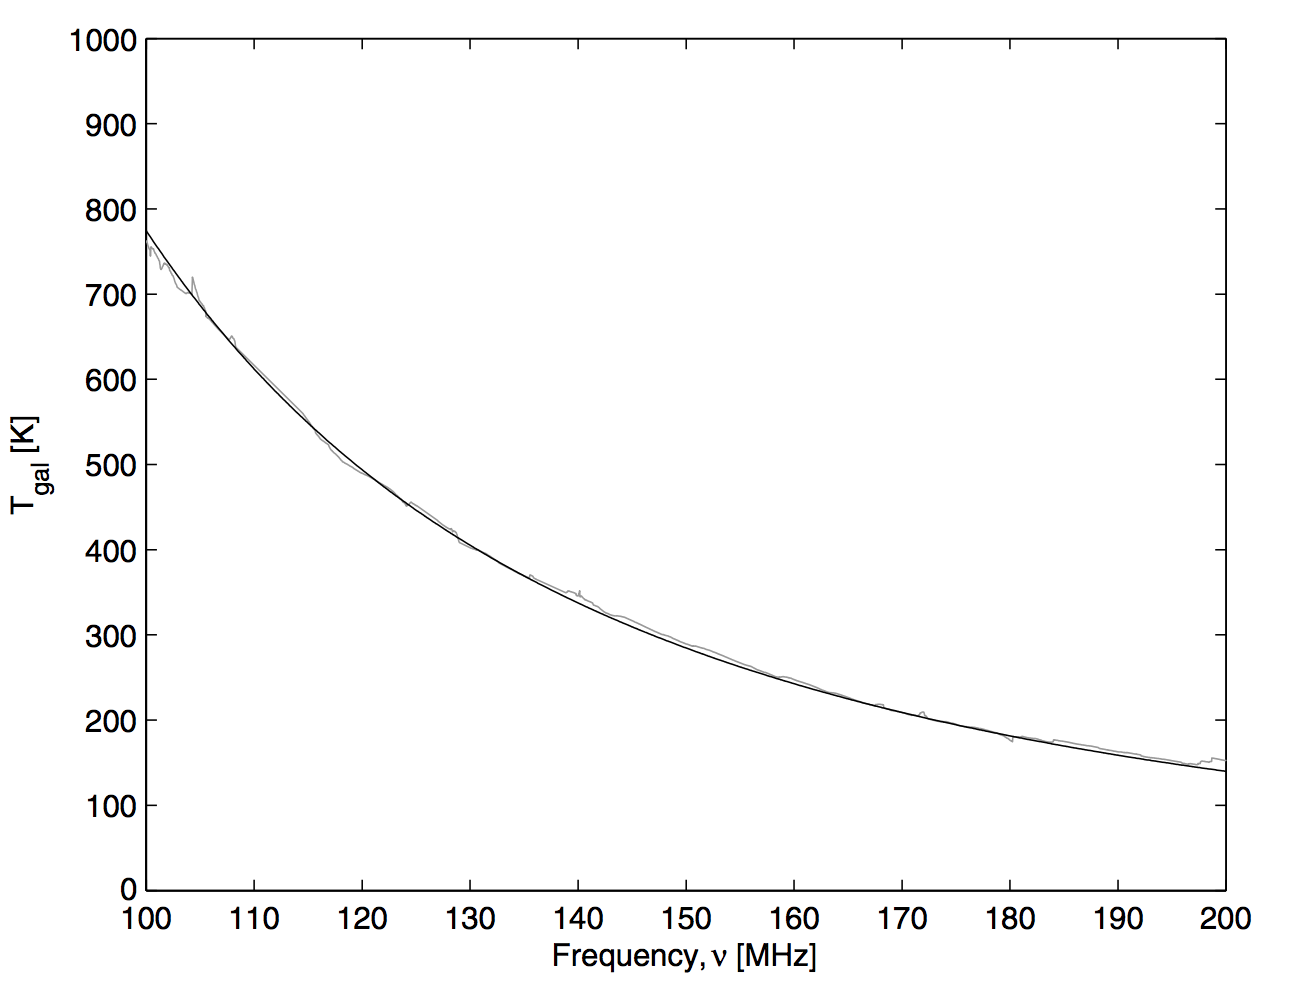
\includegraphics[width=0.75\textwidth]{chapters/astropol/figures/edges_spectrum.png}
\caption[The low-frequency synchrotron spectrum of the sky, as measured by \cite{Rogers.08}.]{The low-frequency synchrotron spectrum of sky, measured by \cite{Rogers.08}. Their measurement is shown in light grey, overlaid with a well-fit power law of spectral index $2.52\pm0.04$.}
\label{fig:astropol_edges_spec}
\end{figure}

\section{Stokes parameters}

It is extremely unlikely that we will observe radiation from electrons spiralling along magnetic field lines that are exactly parallel or perpendicular to our line-of-sight. Instead, some elliptically polarized component of the radiation is observed. The Stokes parameters are quantities used to describe the polarization state of electromagnetic waves.

We can describe a monochromatic electromagnetic wave propagating towards the observer as the real part of 
\begin{equation}
\vec{E} = \vec{E}_0e^{-i\omega t} = \begin{pmatrix}
E_1 e^{i\phi_1}\\
E_2 e^{i\phi_2}
\end{pmatrix}e^{-i\omega t}
\end{equation}
It can be shown \citep[e.g.][]{Rybicki.79} that the real part of the vector above can be mapped, in general, to the principle axes of an ellipse at position angles $\psi$ and $\chi$ to the Cartesian plane, as shown in Figure~\ref{fig:astropol_pol_ellipse}. These two angles, $E_1$, and $E_2$, can be used to define the Stokes parameters for monochromatic waves:
\begin{align}
I &\equiv E_1^2 + E_2^2 = E_0^2, \\
Q &\equiv E_1^2 - E_2^2 = E_0^2\cos 2\psi \cos 2\chi,\\
U &\equiv 2E_1E_2\cos(\phi_1 - \phi_2) = E_0^2\cos 2\chi \sin 2\psi, \\
V &\equiv 2E_1E_2\sin(\phi_1 - \phi_2) = E_0^2\sin 2\chi.
\end{align}

The interpretation of these parameters is as follows: Stokes I measures the total intensity of the electric field. Stokes Q and U measure the orientation of the electric field relative to, in this case, the $x$-axis of the Cartesian plane, where Q measures the projection parallel to the $x$-axis and U measures the projection at $45^{\circ}$ to the $x$-axis. They are clearly linked, as $\tan\psi = U/Q$. Stokes V is the circularity parameter, measuring the ratio of the principle axes of the ellipse. For monochromatic waves, $I^2 = Q^2 + U^2 + V^2$.

\begin{figure}
\centering
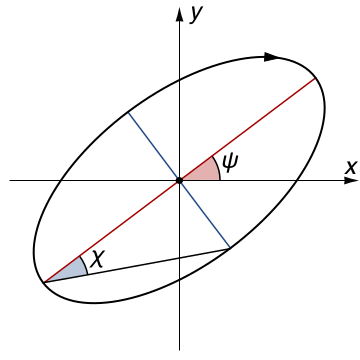
\includegraphics[width=0.5\textwidth]{chapters/astropol/figures/pol_ellipse.png}
\caption{A representation an elliptically polarized monochromatic wave with respect to the Cartesian grid.}
\label{fig:astropol_pol_ellipse}
\end{figure}

In practice, observed radiation fields are rarely monochromatic (purely elliptically polarized). Instead, we observe a superposition of electric fields, each with its own polarization state. If we assume that the amplitude and phase of the observed radiation change relatively slowly over time, we can express 

\begin{equation}
\vec{E}(t) = \vec{E}_0(t)e^{-i\Phi(t)} = \begin{pmatrix}
E_1(t) e^{i\phi_1(t)}\\
E_2(t) e^{i\phi_2(t)}
\end{pmatrix}
\end{equation}
such that over short times $\Delta t \sim 1/\omega$ the wave is of a definite elliptical polarization state, but for $\Delta t \gg 1/\omega$ the polarization state can change by a large amount. Such waves are referred to as `quasi-monochromatic', with coherence time $\Delta t$ and its conjugate, bandwidth $\Delta\omega$. Due to the time-dependent nature of quasi-monochromatic waves, the exact values of $E_1$, $E_2$, $\phi_1$ and $\phi_2$ cannot be precisely measured. Instead, radiometers measure the average sum of squares of the components of $\vec{E}(t)$. These can be used to define the Stokes parameters for quasi-monochromatic waves:

\begin{align}
I &\equiv  \left\langle E_1E_1^* \right\rangle + \left\langle E_2E_2^* \right\rangle = \left\langle E_1^2 + E_2^2 \right\rangle, \\
Q &\equiv \left\langle E_1E_1^* \right\rangle - \left\langle E_2E_2^* \right\rangle = \left\langle E_1^2 - E_2^2 \right\rangle, \\
U &\equiv \left\langle E_1E_2^* \right\rangle + \left\langle E_2E_1^* \right\rangle = \left\langle 2 E_1 E_2 \cos(\phi_1 - \phi_2)\right\rangle, \\
V &\equiv -i (\left\langle E_1E_2^* \right\rangle - \left\langle E_2E_1^* \right\rangle) = \left\langle 2 E_1 E_2 \sin(\phi_1 - \phi_2)\right\rangle, \\
\end{align}
where $E_i^*$ indicates the complex conjugate of $E_i$, and $\left\langle \cdots \right\rangle$ indicates an average over some integration time over which the measurement is made. It is easy to see from the Cauchy-Schwarz inequality that for quasi-monochromatic waves, $I^2 \geq Q^2 + U^2 + V^2$. Radiation is completely unpolarized if $Q=U=V=0$. It it common to refer to the ``polarization fraction'' or ``degree of polarization'' of observed radiation, $p$:

\begin{equation}
p \equiv \frac{\sqrt{Q^2 + U^2 + V^2}}{I}
\end{equation}
and ``linear polarized intensity'', $P$:

\begin{equation}
P = \frac{1}{2}\sqrt{Q^2 + U^2}
\end{equation}

The Institute of Electrical and Electronics Engineers (IEEE) defines the standard reference frame for the polarization axes to be the lines of constant Right Ascension ($\alpha$) and Declination ($\delta$) on the sky. Substitution of $1\rightarrow\alpha$ and $2\rightarrow\delta$ in the definitions above brings those definitions to standard \citep{Cohen.58, Ludwig.73, vanStraten.10}.

\section{Total intensity foregrounds}

At EoR frequencies, $50 - 250$\,MHz, the brightest source of total intensity is the Galactic Plane. While the configuration of the Galactic magnetic field is still a matter of debate \citep[e.g.][]{Haverkorn.15}, but observations of synchrotron emission suggest it has an average power of $\sim6\mu$G \citep[e.g.][]{Beck.03}. Multiple, dynamic sources of {\sc hii} such as supernova remnants (SNRs) and other contributors to the interstellar medium provide charged particles to radiate synchrotron. This has a brightness temperature of $\sim$5\,K. Beyond our Galaxy, synchrotron from extragalactic sources (galaxies and galaxy clusters) have brightness temperatures $\sim$0.5\,K \citep[e.g.][]{Jelic.10}. 

With the advent of newly operational low-frequency interferometers (see Chapter~\ref{chapter:instruments}), detailed maps of low-frequency synchrotron emission in the Southern Hemisphere have only very recently become accessible. 
The PAPER-64 imaging array \citep[][and Chapter~\ref{chapter:instruments}]{Jacobs.11, Jacobs.13, Stefan.13} was used to make a map of the Southern Galactic Plane at 145\,MHz. This array was able to resolve some diffuse components, but mainly focused on relatively small-scale structures such as SNRs and {\sc hii} regions (i.e. tens of parsecs; \citealt{Asvarov.13}). That map is shown in Figure~\ref{fig:astropol_galplane_paper}, projected into Galactic coordinates. Synchrotron sources in the plane of the Galaxy include SNRs (most prominently the Vela and Puppis complexes to the East), {\sc hii} regions (almost indistinguishable from SNRs in the plane) and ionized gas. Above and below the Galactic plane, extragalactic point sources are visible (and match the \cite{Jacobs.11} 145\,MHz point-source catalog of the region).

\begin{figure}
\centering
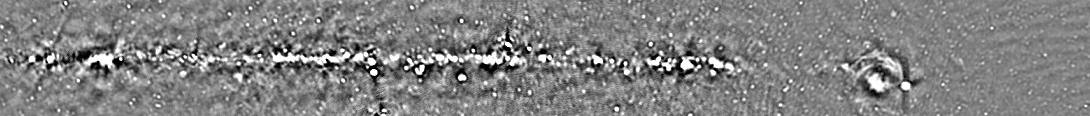
\includegraphics[width=0.9\textwidth]{chapters/astropol/figures/galplane_linscale.png}
\caption[The Southern Galactic Plane as observed by PAPER-64 at 145\,MHz.]{The Galactic plane as observed by PAPER-64. Synchrotron sources include supernova remnants (e.g. the Vela and Puppis complexes to the East), {\sc hii} regions and ionized gas in the plane of the Galaxy. Extragalactic sources are visible above and below the Galactic plane.}
\label{fig:astropol_galplane_paper}
\end{figure}
% GSM -- collection of data including very diffuse components
Motivated by the sparsity of wide-field, diffuse radio surveys, \cite{GSM.08} presented the `Global Sky Model' (GSM), in which they amalgamated as many high-fidelity wide-field radio surveys as possible, from 10\,MHz to 100\,GHz. \cite{GSM.17} extended the upper limit of this range to 10\,THz. Using principal component analysis and an expectation for smooth frequency structure, they were able to build a model that could be interpolated to any requested frequency within their spectral range. An example at 150\,MHz is shown in Figure~\ref{fig:astropol_gsm}. It is important to note that the GSM is uncertain at the $\sim$5\% level, and in the southern hemisphere this uncertainty is greater due to fewer well-characterized surveys of diffuse emission. Aside from diffuse Galactic emission, the GSM also includes the `A Team' of bright radio sources, such as Pictor A, Fornax A and Centaurus A. Pictor A is particularly useful as a calibration source: it is relatively unpolarized, unresolved as a point source, and the one of the brightest extragalactic sources of synchrotron emission \citep{Jacobs.13}.

\begin{figure}
\centering
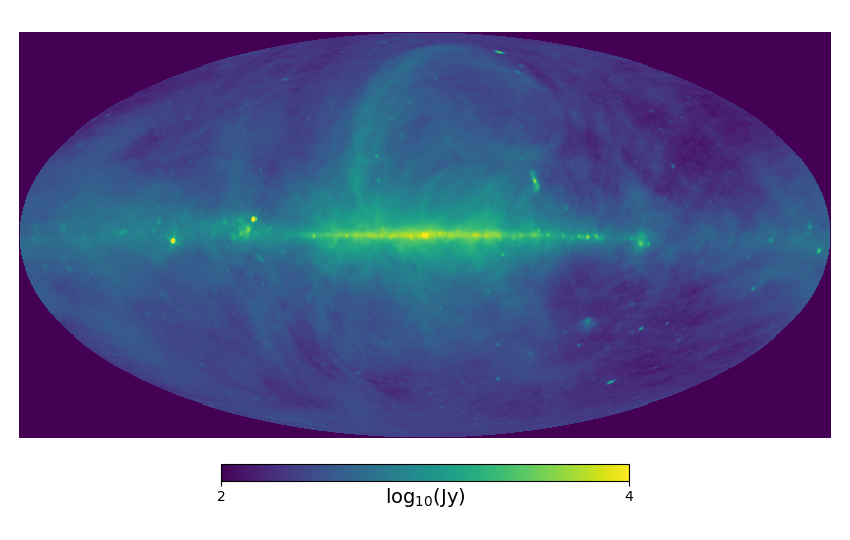
\includegraphics[width=0.75\textwidth]{chapters/astropol/figures/gsm.png}
\caption{The GSM at 150\,MHz: a relatively accurate model of diffuse synchrotron across the entire sky.}
\label{fig:astropol_gsm}
\end{figure}

With the advent of the 128-tile Murchinson Widefield Array (MWA), the GaLactic and Extragalactic All-sky Murchison Widefield Array (GLEAM) survey took place over two years, imaging most of the sky south of Declination $+25^{\circ}$ in Stokes I, Q, U \& V with myriad science goals \citep{Bowman.13, Wayth.15, Hurley-Walker.17}. Covering 70--230\,MHz with 10\,kHz frequency resolution, sensitivity to a wide range of spatial scales, and reaching theoretical noise levels in Stokes I, GLEAM (the maps of which are not yet public) will have a significant legacy for our understanding of the low-frequency sky. 

\section{Linearly Polarized Foregrounds}
\label{sec:astropol_linpol_fgs}
Polarized foregrounds are less well characterized than total intensity ones, especially in the southern hemisphere, and even then, the measurements were typically at GHz frequencies and must be extrapolated for relevance to EoR studies. The DRAO 26\,m \citep{Wolleben.06} telescope and the VLA \citep{Condon.98} mapped the entire sky, in Stokes I, Q, U \& V, visible from their respective positions in the northern hemisphere. This meant that much of the southern hemisphere was blocked by the Earth. Both of these surveys were performed at 1.4\,GHz. The polarized intensity map produced by \cite{Wolleben.06} is shown in Figure~\ref{fig:astropol_drao_map} in Galactic coordinates.

\begin{figure}
\centering
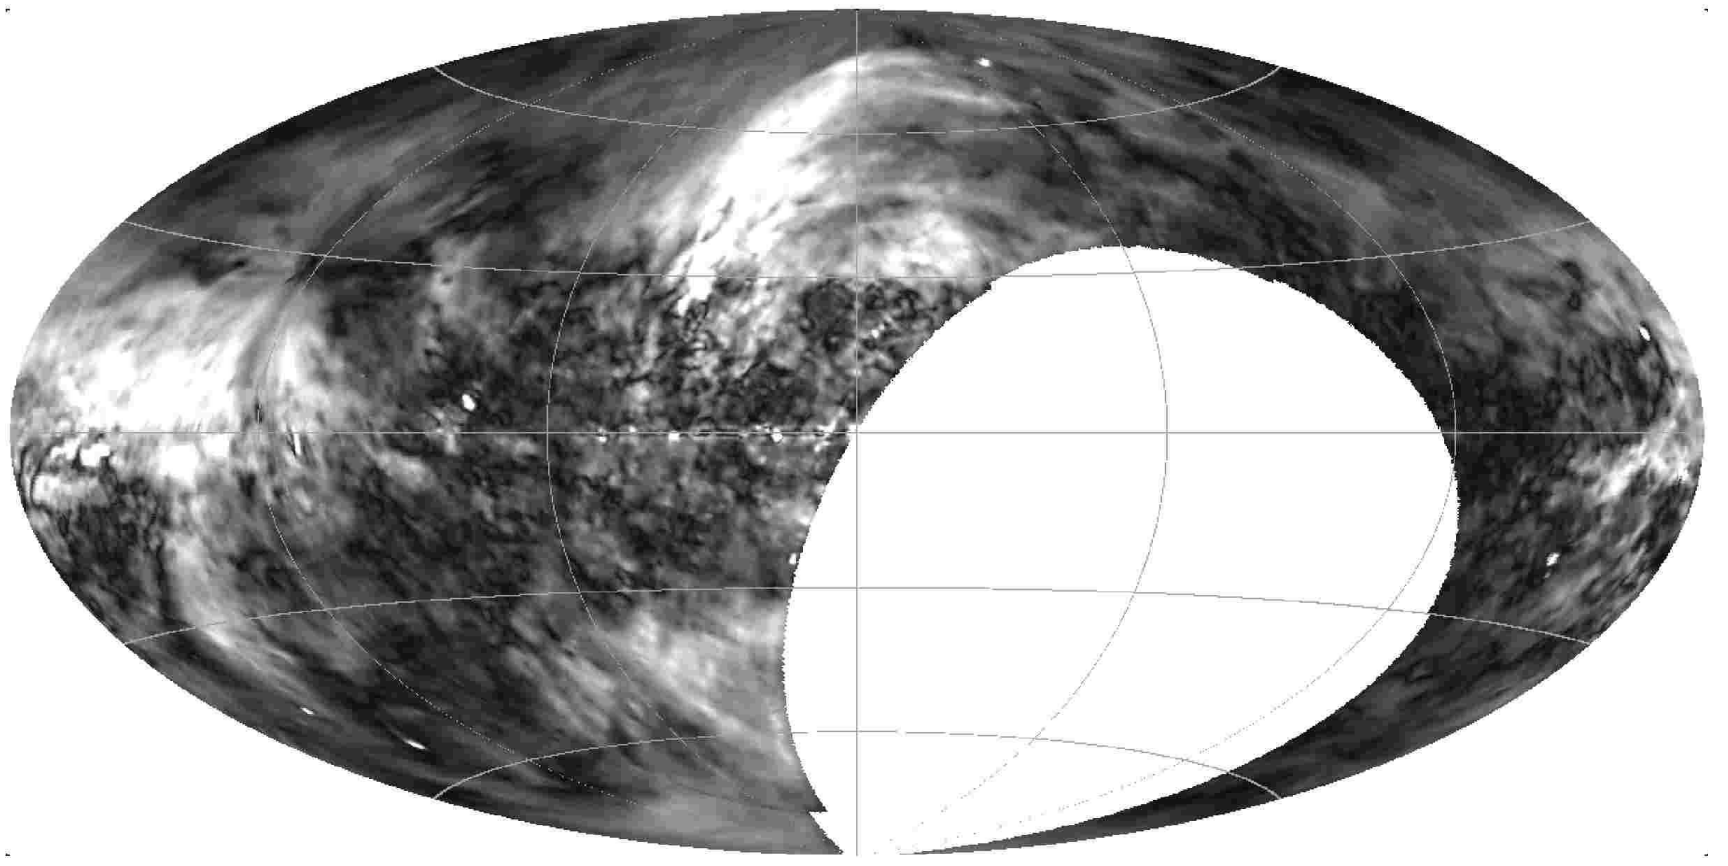
\includegraphics[width=0.7\textwidth]{chapters/astropol/figures/drao_map.png}
\caption{The polarized intensity of the sky as viewed by the DRAO 26\,m telescope at 1.4\,GHz. Figure taken from \cite{Wolleben.06}.}
\label{fig:astropol_drao_map}
\end{figure}

\cite{Bernardi.13} surveyed 2400\,deg$^2$ of the southern hemisphere with the 32-element MWA at 189\,MHz in Stokes I, Q and U. They detected large amounts of bright ($\sim 10$\,K), diffuse polarized emission at hour angles close to the transit of the Galaxy (most likely the contribution of diffuse emission south of the Galactic Plane, as visible in Figure~\ref{fig:astropol_drao_map}), but just one polarized extragalactic source with flux density $>4$\,Jy. 

Indeed, most recent observations in the 100--200 MHz band, covering selected sky areas, have revealed that bright Galactic diffuse polarized synchrotron radiation seems to be ubiquitous \citep{Bernardi.09, Bernardi.10, Jelic.14, Lenc.16} with peak emission up to 15 K \citep{Jelic.15}, but find a dearth of bright polarized (extragalactic) point sources. The point sources cataloged by \cite{Bernardi.13} showed significant depolarization compared to their polarized flux density at higher frequencies (see Section~\ref{subsec:astropol_depolar}). 

As calibration schemes are refined and modern interferometers grow, a small population of weakly polarized point sources has recently been revealed. Observing $\sim 625$\,deg$^2$ with the 128-element MWA, at 154\,MHz, \cite{Lenc.16} found five polarized point sources of polarized intensity order $10-100$\,mJy\,beam$^{-1}$. Much deeper integrations with the Low Frequency Array (LOFAR) presented by \cite{VanEck.18} found 92 polarized point sources within 570\,deg$^2$, observed at 150\,MHz, with polarized intensities of the  order $1-10$\,mJy\,beam$^{-1}$. In all of these observations, polarized intensity represented a polarized fraction $p\leq 15$\%.

Note that we have focused on polarized intensity -- Stokes Q and U -- for this discussion.
At low frequencies, Stokes V is expected to be almost intrinsically zero \citep[e.g.][]{Sokolowski.17}. While at higher frequencies circularly polarized synchrotron has been observed from sources such as relativistic jets \citep[e.g.][]{Macquart.04}, very few natural sources of Stokes V are present in the low frequency sky, with the exception of transients such as extrasolar flares \citep{Spreeuw.10} and aurorae of giant planets \citep[e.g.][]{Zarka.05, Badman.15}. This makes measurements of Stokes V useful for null tests \citep[e.g.][]{Patil.17}

\subsection{Faraday Rotation}

One of the most important considerations for {\sc hi} EoR measurements is the Faraday Rotation Measure of polarized foregrounds (the reasons for this are thoroughly enumerated in Chapter~\ref{chapter:eor_window_theory}). 

Electromagnetic waves will undergo dispersion and refraction while propagating through and ionized gas or plasma. If an external magnetic field is incident upon the plasma, electrons in the plasma will gyrate about the field with frequency
\begin{equation}
\omega_B = \frac{e}{m_e c}B_0 \approx 1.67\times 10^7 B_0 {\rm\, s^{-1}},
\end{equation}
where $B_0$ is the magnitude of the magnetic field. This alters the dielectric constant in the plasma.
Decomposing linearly polarized radiation in to a circular basis (this basis change is not the equivalent of intrinsically circularly polarized Stokes V radiation) of clockwise (`right-handed'; R) and anti-clockwise (`left-handed'; L) waves, we can express the dielectric constant as
\begin{equation}
\epsilon_{R,L} = 1 - \frac{\omega_P^2}{\omega(\omega \pm \omega_B)},
\end{equation}
where R and L correspond to + and -, respectively, $\omega$ is the angular frequency of the radiation, and $\omega_P$ is the plasma frequency
\begin{equation}
\omega_P^2 = \frac{4\pi n_e e^2}{m_e},
\end{equation}
for electron number density $n_e$. The index of refraction of a plasma is given by $\sqrt{\epsilon}$. Clearly, the handedness of the radiation will experience different angles refraction. The effect of this in the linear basis is to rotate the plane of polarization as the radiation propagates through the magnetized plasma. For a screen of width $L$, the change in angle is given by \citep{Rybicki.79, TMS}:
\begin{equation}
\Delta\phi = \frac{1}{2}\int^L_0 \frac{\omega_P^2\omega_B}{c\omega^2}{\rm d}l.
\end{equation}
Substituting for $\omega_B$ and $\omega_P$, and observing the radiation along the line-of-sight (as we must), gives
\begin{equation}
\Delta\phi = \frac{e^3}{(m_e c^2)^2}\lambda^2 \int^L_0 n_e(l)B_{\parallel}(l) {\rm d}l \equiv \lambda^2\Phi
\end{equation}
where we have moved from angular frequency to wavelength, and defined the \textit{Faraday Rotation Measure} (RM) $\Phi$. This rotation moves power between Stokes Q and U,
\begin{equation}
(Q + iU)_{\rm observed} = e^{-2i\Phi\lambda^2}(Q + iU)_{\rm intrinsic},
\label{eq:astropol_faraday_rotation}
\end{equation}
where $\Phi$ has units of rad\,m$^{-2}$.

At GHz radio frequencies, measurements of polarization angle with respect to wavelength can be used to chart the magnetic field of galaxies, given some independent measure of the electron number density. Equation~\ref{eq:astropol_faraday_rotation} also defines a Fourier relationship between $\Phi$ and $\lambda^2$, which can be exploited to obtain a similar measurement, and is referred to as `RM synthesis' \citep{Brentjens.05}. Importantly, at low frequencies the large values of $\lambda$ will cause rapid phase wraps for RMs $\geq \sim 10$, inducing spectral structure in what would otherwise be smooth synchrotron spectra \citep{Moore.13}. 

Figure~\ref{fig:astropol_rm_map} shows the all-sky RM measurements of \cite{Oppermann.12}, obtained by using both of the above methods (fitting in $\lambda^2$ and RM synthesis) on a number of radio surveys ranging from $1.1$ to $11$\,GHz. Uncertainties in the values reported are typically at the level of $\sim$10\%, with larger uncertainties in the southern hemisphere due to fewer polarization surveys existing in that region, and along the Galactic plane. 

\begin{figure}
\centering
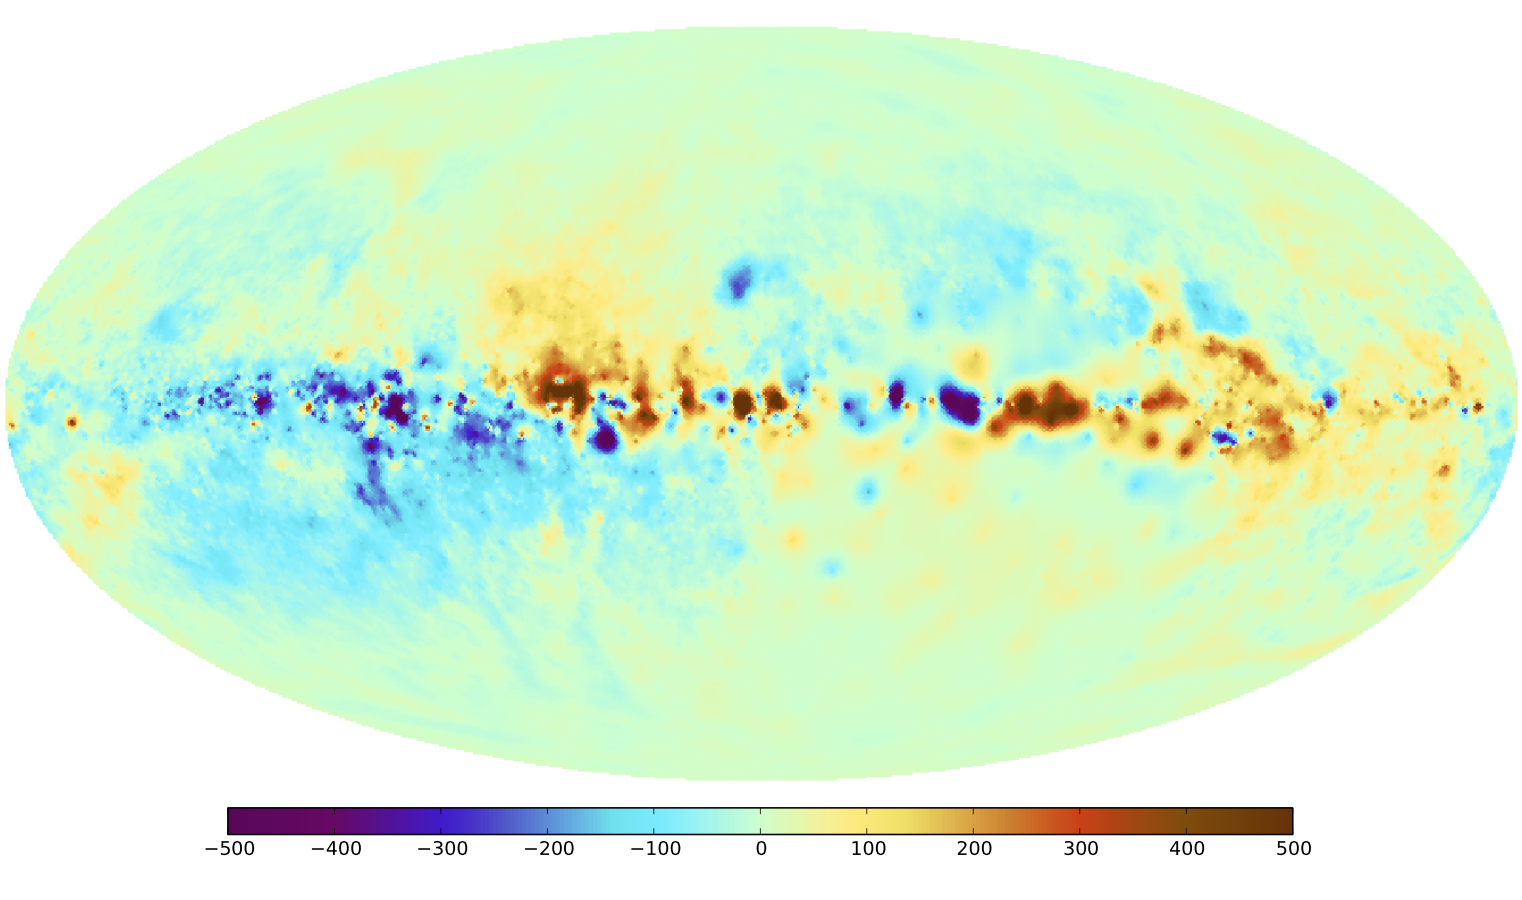
\includegraphics[width=0.7\textwidth]{chapters/astropol/figures/oppermann_map.png}
\caption[An all-sky map of RMs.]{An all-sky map of RMs. The colorbar has units of rad\,m$^{-2}$. Figure taken from \cite{Oppermann.12}.}
\label{fig:astropol_rm_map}
\end{figure}

\subsection{Depolarization}
\label{subsec:astropol_depolar}

Frequently the intrinsic polarization fraction of a radiating source much greater than the observed value; the observed radiation is `depolarized'. Modes of depolarization can generally be categorized in to two groups: natural and instrumental. 

Instrumental polarization can occur via the beam -- the receptivity pattern, or point spread function (PSF) -- of the instrument (see Chapter~\ref{chapter:interferometry}). If the polarization angle changes significantly within the area of the beam, which is the case for turbulent Galactic magnetic fields and the very large beam areas of modern instruments (e.g. Chapter~\ref{chapter:instruments}), the observed polarization fraction can be attenuated during integration over the beam area. 
When probing RM distributions via RM synthesis, the channel width over which the data are averaged sets the sensitivity to the maximum RM by definition. Sources with higher RMs will suffer from `bandwidth depolarization', and this effect will strengthen at lower frequencies according to the phase-wrapping factor $2\Phi\lambda^2$.
As we explore in the next Chapter, interferometric polarization measurements are obtained by measuring the projection of the electric vector field on to orthogonal dipole arms. An electrical phase offset between the two arms will almost certainly exist in any instrument. If left uncalibrated, Stokes U will leak in to Stokes V, consequently depolarizing linear polarized intensity. Likewise, relatively faint polarized emission can be ``washed-out'' of measurements if Stokes I is able to leak in to Stokes Q and U measurements.

Natural depolarization can arise at the source of the radiation, due to turbulent magnetic fields. Different magnetic field projections along the line-of-sight can produce different angles of polarization, that can on average attenuate the observed polarized intensity. Similarly, radiation emitted from different depths of the source can undergo different amounts of Faraday rotation along the line-of-sight as they pass through regions of different electron densities. This effect is apparent in Figure~\ref{fig:astropol_drao_map}: in the plane of the Galaxy, which has a large column depth, the observed polarized intensity is low compared to, for example, the Northern Galactic Spur, which is physically closer to the Earth. 

Finally, the ionosphere of the Earth is a turbulent plasma, which when coupled with the Earth's magnetic field can act as a Faraday screen. If left uncorrected, averaging observations of the same patch of sky observed at different times can lead to a depolarization effect -- we explore this further in Chapter~\ref{chapter:ionosphere}.

As mentioned in Section~\ref{sec:astropol_linpol_fgs}, \cite{Bernardi.13} reported polarization fractions of extragalactic compact sources at 189\,MHz significantly lower than reported at higher frequencies. This was corroborated by some of the  measurements by \cite{Lenc.16}, although not all of the polarized point sources found in their survey showed significant evidence of depolarization. The least depolarized sources in that survey corresponded to hot-spots of large radio galaxies, which perhaps are not as deeply embedded in galactic plasma as the other sources observed, and therefore suffered less natural depolarization. \cite{Farnes.14} showed a systematic trend for depolarization of steep-spectrum point sources as frequency decreased, resulting in very low polarization fractions ($\ll 1\%$) below 300 MHz. They also suggested that natural polarization was the cause, due to turbulent magnetic fields at the source of the radiation.\\\\

Recall that in Chapter~\ref{chapter:eor_intro}, we stated that 21\,cm emission was effectively unpolarized. Why have we gone in to so much detail about polarized radiation? As we will see in subsequent Chapters, polarized power is capable of `leaking' in to Stokes I measurements through effects intrinsic to radiometric instruments, and calibration errors. Recall also that Faraday Rotation can induce spectral structure in otherwise smooth spectrum, polarized synchrotron emission. Coupled with leakage, this additional spectral structure risks contaminating the one lever-arm we have against the bright foregrounds! This effect lead to much of the research presented in this work.
 % Astrophysical Radiation
%
% synchtrotron & bremstrahlung
% GSM 2008, 2017
% what is polarization (emag)
% sources of astrophysical polarization
% magnetic fields and rotation measures
% oppermann map -- high RM point sources
% Lenc, Jelic, etc. diffuse low RM stuff
%
\chapter{Interferometry, Calibration \& Polarimetry}
\label{chapter:interferometry}

In this Chapter I wished to build a formalism around wide-field, polarized interferometric measurements that could be used throughout this work. Many traditional assumptions used in radio interferometry are broken in the case of the wide-field, fully-polarized, drift-scanning measurements native to interferometric EoR observations. In Section~\ref{sec:interferometry_vis}, I derive the equation describing the fundamental observable for an interferometer, called a ``visibility". Section~\ref{sec:interferometry_cal}, I describe calibration techniques relevant to this work and in Section~\ref{sec:interferometry_pol} I review some of the implications of the previous two sections for polarized measurements.

For a comprehensive review of interferometry from a traditional perspective, see \cite{TMS}.

\section{The Visibility Equation}
\label{sec:interferometry_vis}

A radio interferometer (a term used interchangeably with ``interferometric array" for radio observations) is an ensemble of receiving elements, where each element's measurement is correlated with every other element's. The simplest case is a two-element interferometer, which we will focus on below. We assume that the elements are coplanar and identical.

\subsection{The Classical Visibility Equation}

Consider two receiving elements $i$ and $j$, separated by baseline vector $\vec{b}$. Suppose a plane wave of wavelength $\lambda$ is incident upon these elements, with direction of propagation $-\hat{s}$. The geometry of this interferometer is illustrated in Figure~\ref{fig:interferometry_2element}.

\begin{figure}
\centering
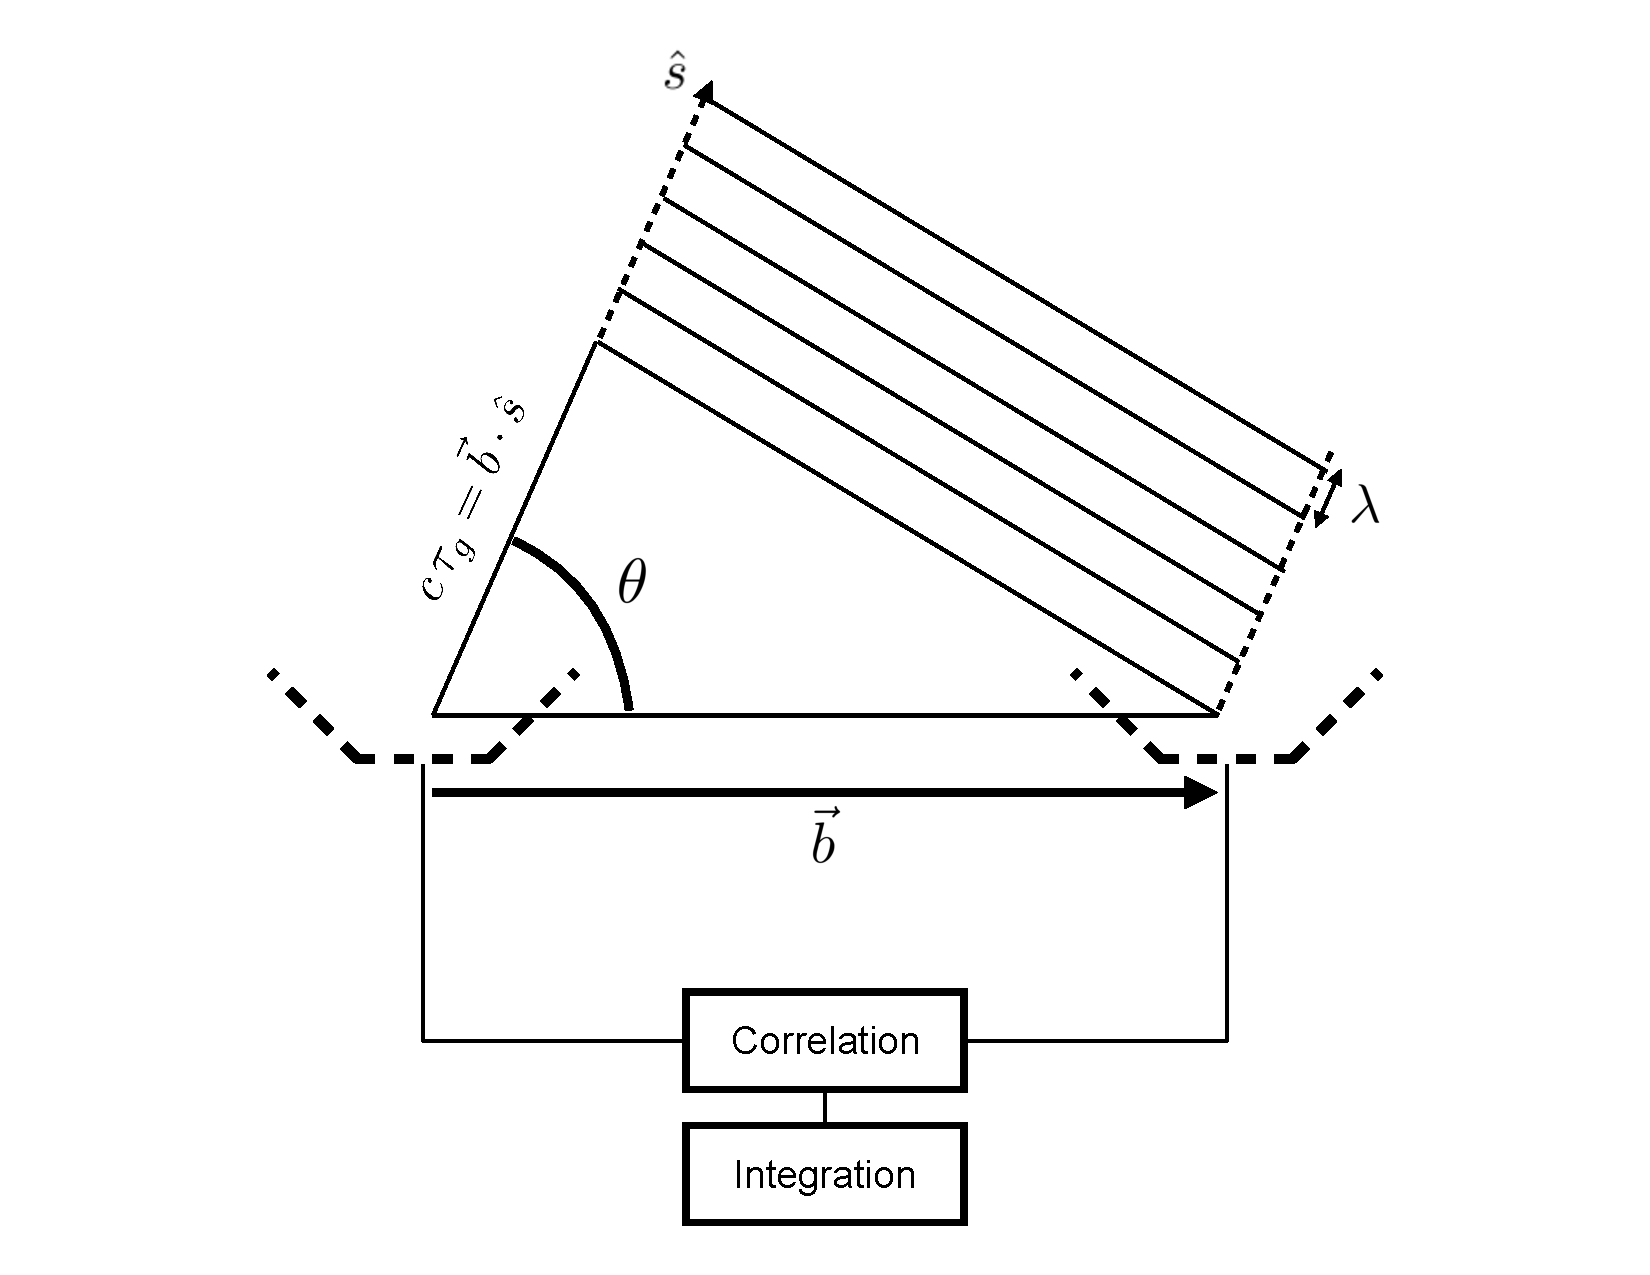
\includegraphics[width=0.9\textwidth]{chapters/interferometry/figures/visibility_explanation.pdf}
\caption{The geometry of a two-element interferometer, with a plane wave incident from direction $\hat{s}$.}
\label{fig:interferometry_2element}
\end{figure}

We can define the electromagnetic wave to have a frequency dependent phase, such that the electric field measured by element $i$ at time $t$ is

\begin{equation}
E_i = E_0 e^{-2\pi i \nu t}.
\label{eq:Ei}
\end{equation}

The time difference between the arrival at $i$ and $j$ is called the ``geometrical delay", $\tau_g$:

\begin{equation}
\tau_g = \frac{\vec{b}\cdot\hat{s}}{c},
\end{equation}
and the electric field measured by element $j$ is

\begin{equation}
E_j = E_0 e^{-2\pi i \nu (t+\tau_g)}.
\end{equation}

An interferometer is an instrument which measured voltages induced by these electric fields, and correlates them together, integrating their product over some coherent time-scale. This correlation grants:

\begin{equation}
\langle E_i E_j^* \rangle 
= \lim_{T\rightarrow\inf}\frac{1}{2T}\int^T_{-T} E_i(t) E_j(t) {\rm d}t
= | E_0 |^2 e^{-2\pi i \nu \tau_g}
\label{eq:vis_time_integration}
\end{equation}
where $e^{-2\pi i \nu \tau_g} = e^{-2\pi i \nu \vec{b}_{ij}\cdot\hat{s}/c}$ is known as the ``fringe" term, due to its sinusoidal nature. We can generalize this relationship to include more than a single plane wave from direction $\hat{s}$. Many plane waves, from all directions, can be incident upon the interferometer at a given time and frequency. We can represent the power distribution on the sky as $S(\Omega)$, where $S(\Omega)$. However, no instrument is equally sensitive to radiation from every direction $\hat{s} \in \Omega$. Instead, an instrument has some sensitivity pattern -- a \textit{beam pattern} -- that tapers the power distribution on the sky into an ``observed sky",  $S'(\Omega) = A(\Omega)S(\Omega)$. 

These generalizations lead to the classical visibility equation:

\begin{equation}
V_{ij}(\nu) = \int A(\Omega, \nu) S(\Omega, \nu) e^{-2\pi i \nu \vec{b}_{ij}\cdot\hat{s}/c} {\rm d}\Omega
\label{eq:classical_visibility}
\end{equation}
for a ``visibility" -- the fundamental interferometric observable -- $V_{ij}$ as a function of frequency.

If we choose to represent the source direction in terms of directional cosines $\ell$ and $m$, and represent the baseline vector in units of wavelengths, $\vec{b}_{ij}/\lambda=(u,v,w)$, we can perform a change of variables in Equation~\ref{eq:classical_visibility} to give

\begin{equation}
V_{ij}(u,v) = \int\int A(\ell, m)S(\ell, m) e^{-2\pi i (u\ell + vm + w\sqrt{1 - \ell^2 - m^2})} \frac{ {\rm d}\ell {\rm d}m }{\sqrt{1 - \ell^2 - m^2}}.
\label{eq:vis_def_widefield}
\end{equation}

This relationship is often simplified by assuming only a small area of the sky is under observation -- that is, that $A(\ell,m)$ falls-off steeply from zenith -- and therefore $\ell^2$ and $m^2$ are small. This grants

\begin{equation}
V_{ij}(u,v) \approx e^{-2\pi i w} \int\int A(\ell, m)S(\ell, m) e^{-2\pi i (u\ell + vm)} {\rm d}\ell {\rm d}m,
\label{eq:vis_dev_narrowfield}
\end{equation}
which plainly casts $V(u,v)$ as the Fourier transform of the observed sky if $w$ is small: that is, the array is co-planar and no appreciable curvature of the sky is probed. Modern low frequency interferometers used in this work greatly violate this approximation, the consequences of which I will discuss in the proceeding sections.

Even though it is often violated, the Fourier relationship shown in Equation~\ref{eq:vis_dev_narrowfield} is an extremely useful one to work with when translating between visibilities and images. Images can be created by inverse Fourier transforming all of the visibilities measured by an array. Following Equation~\ref{eq:vis_def_widefield}, a reconstructed image $\tilde{S}(\ell, m)$ is given by

\begin{equation}
\frac{A(\ell, m)\tilde{S}(\ell, m)}{\sqrt{1 - \ell^2 - m^2}} = \int\int \Xi(u, v) V(u,v) e^{2\pi i \nu (u\ell + vm)} {\rm d}u {\rm d}v.
\label{eq:image_estimate}
\end{equation}

In Equation~\ref{eq:image_estimate}, we see that the reconstructed image $\tilde{S}(\ell, m)$ is attenuated by the beam response $A(\ell, m)/\sqrt{1 - \ell^2 - m^2}$. The function $\Xi(u, v)$ defines the sampling of the $u,\,v$ - plane. It is equal to 1 at the points sampled by the interferometer (baselines of length and direction defined by the vector  $\vec{b} = (u,v)$ exist in the array) and 0 elsewhere. As an example, the ``array" shown in Figure~\ref{fig:interferometry_2element} would be described by a $\Xi(u, v)$ function that was zero at all points except for a single ($u,\,v$) coordinate described by baseline vector $\vec{b}$.

The effect of the sampling function $\Xi(u, v)$ is that the true sky $S(\ell,m)$ can never be completely reconstructed, since it is impossible to build an interferometer that samples every $u,v$ mode. The true sky is convolved with the Fourier transform of $\Xi(u, v)$, which astronomers refer to as the ``dirty beam". $\Xi(u, v)$ contains zeros, so a complete deconvolution of $\tilde{S}(\ell, m)$ is impossible.

We now note that an important aspect of light has been absent throughout the derivations above: the polarization state of the radio wave that induces the electric field in Equation~\ref{eq:Ei}. Interferometers are typically constructed with two feeds, sensitive to polarization states of an incident radio wave along two separate axes. In the case of all of the instruments used in this work (see Chapter~\ref{chapter:instruments}), an antenna $i$ had two dipole feeds perpendicular to one another. These were along the North-South direction (`n') and the East-West direction (`e'). We can attempt to generalize Equation~\ref{eq:classical_visibility} to include polarization, setting antenna $i$ to have orientation $p$ and antenna $j$ to have orientation $q$, $p,q\in(e,n)$:

\begin{equation}
V^{pq}_{ij} = \int A_{pq}(\Omega, \nu) S_{pq}(\Omega, \nu) e^{-2\pi i \nu \vec{b}_{ij}\cdot\hat{s}/c} {\rm d}\Omega.
\end{equation} 
However, two aspects of this equation are unsatisfactory. As explored in Chapter~\ref{chapter:astro_rad}, the polarized sky is defined with the four Stokes parameters; an ``$S_{pq}$" polarized sky does not exist. Likewise, a dipole is not purely sensitive to a single vector orientation from the sky, but probes a wide range of angles\footnote{In the case of the PAPER instrument, described in the next Chapter, the dipole feeds probed the entire hemisphere of the sky.}. Therefore a $A_{pq}$ polarized beam is ill-defined. These shortcomings lead us to rewrite the visibility equation, cohesively including polarization from the outset.  

\subsection{The Measurement Equation}

The Radio Interferometric Measurement Equation (RIME) provides an extremely useful framework for describing wide-field polarized observations. Formulated by \cite{HBS.1.96}, it was re-introduced to the radio astronomy community through a series of papers by O.~M. Smirnov \citep{Smirnov.11, Smirnov.11.2, Smirnov.11.3, Smirnov.11.4}. In this section I review the portions of his work most relevant to this thesis, and defer the reader to the series for a useful and thorough walk-through of wide-field radio interferometry and high dynamic-range calibration.

Returning to Equation~\ref{eq:Ei}, a radio wave incident on an antenna induces a voltage in along feed arm

\begin{equation}
\vec{E} = (e_p, e_q);\,\,\,\vec{v} = (v_p,v_q) = \textbf{J}\vec{E}
\label{eq:voltage_jones}
\end{equation}
where \textbf{J} is a $2\times2$ complex matrix termed the ``Jones matrix" \citep{Jones.41}. Jones matrices represent linear transformations along the signal path, from the emission of the radio wave onwards. Multiple stages along the signal propagation can be represented by multiplying different Jones matrices together as a ``Jones chain", which may be expanded or collapsed as convenient.

Interferometric visibilities are pairwise correlations of the components of $\vec{v}$ between antennas $i$ and $j$, integrated over some small time span (Equation~\ref{eq:vis_time_integration}), which we can represent hold in matrix form (the layout of which will become clear in a moment):

\begin{equation}
\textbf{V}_{ij} = \begin{pmatrix} 
\langle v^p_i v^{p*}_j \rangle & \langle v^p_i v^{q*}_j \rangle \\
\langle v^q_i v^{p*}_j \rangle & \langle v^q_i v^{q*}_j \rangle \\
 \end{pmatrix} = \langle \vec{v}_i \vec{v}^H_j \rangle.
\end{equation}
Above, H represents the Hermitian transpose operation.

Using this formalism allows us to map the emitted electric field to the observed visibilities, 
\begin{equation}
\textbf{V}_{ij} = \textbf{J}_i \begin{pmatrix} 
\langle e^p_i e^{p*}_j \rangle & \langle e^p_i e^{q*}_j \rangle \\
\langle e^q_i e^{p*}_j \rangle & \langle e^q_i e^{q*}_j \rangle \\
 \end{pmatrix} \textbf{J}^H_j = \textbf{J}_i \textbf{C}_{ij} \textbf{J}^H_j
\end{equation}
where \textbf{J}$_{i,j}$ may be Jones chains of arbitrary length. We have assumed instrument stability to move them out of the time averages in the central matrix. We refer to $\textbf{C}_{ij}$ as the ``coherency matrix". 

In Chapter~\ref{chapter:astro_rad} the Stokes parameters we introduced. \cite{Hamaker-Bregman.96} showed that the components of the coherency matrix are closely related to the Stokes parameters:

\begin{equation}
\begin{pmatrix} 
\langle e^p_i e^{p*}_j \rangle & \langle e^p_i e^{q*}_j \rangle \\
\langle e^q_i e^{p*}_j \rangle & \langle e^q_i e^{q*}_j \rangle \\
 \end{pmatrix}
 =
 \begin{pmatrix} 
I + Q & U + iV \\
U - iV & I - Q \\
 \end{pmatrix}.
 \label{eq:interferometry-stokes-coherency}
\end{equation}

The Jones formalism allows for a construction of the visibility equation that does not make explicit assumptions regarding polarization or field-of-view, in which we can map the Stokes parameters into the instrumental basis that visibilities are computed in:

\begin{equation}
\textbf{V}_{ij} = \int \textbf{J}_i(\hat{s}) \textbf{C}_{ij}(\hat{s}) \textbf{J}_j^H(\hat{s}) e^{-2\pi i \nu \vec{b}_{ij}\cdot\hat{s}/c} {\rm d}\Omega,
\label{eq:RIME}
\end{equation}
which \cite{Smirnov.11} refers to as the ``Full Sky Radio Interferometric Measurement Equation"\footnote{We choose to explicitly show the exponent in this formulation for ease of comparison with Equation~\ref{eq:classical_visibility}. \cite{Smirnov.11} shows that this term can written as a ``phase delay Jones matrix" and absorbed into the Jones chain.}. Note that all of these quantities are functions of frequency as well, in general.

So far, the formalism shown has used the $2\times 2$ ``Jones basis". It is sometimes more useful to work in the $4\times 4$ ``Mueller basis" \citep{Mueller.48}, which acts on visibilities in $4\times 1$ vector form:

\begin{equation}
\begin{pmatrix}
V^I \\
V^Q \\
V^U \\
V^V \\
\end{pmatrix}
=
\textbf{S}\vec{V}_{ij}
= 
\begin{pmatrix}
1 & 0 & 0 & 1 \\
-1 & 0 & 0 & 1\\
0 & 1 & 1 & 0 \\
0 & -i & i & 0 \\
\end{pmatrix}
\begin{pmatrix}
V^{pp} \\
V^{pq} \\
V^{qp} \\
V^{qq} \\
\end{pmatrix}.
\label{eq:interferometry_pseudo_stokes}
\end{equation} 

It is important to note that Equation~\ref{eq:interferometry_pseudo_stokes} lists a vector of ``Stokes-polarized visibilities" on the left-hand side, whereas  Equation~\ref{eq:interferometry-stokes-coherency} shows that the coherency matrix contains linear combinations the Stokes parameters. This is not an inconsistency. While visibilities are quantities that are integrated over the sky, the Stokes parameters are only defined \textit{on} the sky. One must transform the visibilities from the $uv$-plane onto the image-plane and deconvolve the beam in order to measure the Stokes parameters. Instead, linear combinations of visibilities measure a proxy for each the Stokes parameters. To make the inequality between visibilities and Stokes parameters explicit, I will refer to the ``Stokes-polarized visibilities" as ``pseudo-Stokes visibilities" from now on.

One can translate between these two formalisms using the definition of $\vec{V}_{ij}$ (c.f. Equation~\ref{eq:voltage_jones}),

\begin{equation}
\vec{V}_{ij} = (\textbf{J}_i \otimes \textbf{J}_j^H)(\vec{E}\otimes\vec{E}^H).
\end{equation}

Comparison of Equation~\ref{eq:classical_visibility} and \ref{eq:RIME} shows that the Jones chain must, at the very least, encapsulate the beam pattern of the instrument. We can build such a Jones matrix by considering the response of feed $p$ on antenna $i$ to an electric field from infinity in the direction ($\theta$, $\phi$):

\begin{equation}
\vec{A}_i^p(\hat{s}) = A^p_{i,\theta}(\hat{s})\hat{\theta} + A^p_{i,\phi}(\hat{s})\hat{\phi},
\end{equation}
where we have suppressed the frequency dependence. The antenna patterns may be written as components of a ``Beam Jones matrix" for an antenna,

\begin{equation}
\textbf{J}_i^{\rm B}(\hat{s}) = 
\begin{pmatrix}
A^p_{i,\theta}(\hat{s}) & A^p_{i,\phi}(\hat{s}) \\
A^q_{i,\theta}(\hat{s}) & A^q_{i,\phi}(\hat{s}) \\
\end{pmatrix}.
\label{eq:jones-beam}
\end{equation}

These are the essential components for understanding the fundamental measurement performed by an interferometer. However, there are several effects one must take into account for the equations to truly reflect an interferometric measurement; effects such as instrumental gains, reflections between antennas, Faraday rotation in the ionosphere, etc. Most importantly, we must consider how these factors affect the measurement of polarization.

\section{Calibration Techniques}
\label{sec:interferometry_cal}

The purpose of calibration is to remove effects of the instrument and the atmosphere from the data. Visibilities are measured in ``data units". That is, a given feed on an antenna will record some measurement of power, but some scalar conversion factor is required to calibrate that power to units of flux density. As visibilities measure the pairwise correlations of antenna powers, the estimation of the calibration factors can quickly become difficult as the number of antennas increases. In this Section we explain different approaches to such a challenge.

\subsection{Diagonal and off-diagonal calibration}

The calibration term that converts the power measured by an antenna to physical units is referred to as the ``antenna gain". This may be summarized per feed as a direction-independent ``Gain Jones matrix",

\begin{equation}
\textbf{J}_i^{\rm G} = 
\begin{pmatrix}
g_i^p &0 \\
0 & g_i^q\\
\end{pmatrix},
\label{eq:jones-gains}
\end{equation}
where we have suppressed the frequency dependence. The components of $\textbf{J}_i^{\rm G}$ are complex numbers, the argument of which represents instrumental phase, and the modulus represents instrumental amplitude. Note that this formulation of $\textbf{J}_i^{\rm G}$ is only appropriate for linear antenna feeds. Circular feeds, which we will not comment on for the rest of this work, require an additional rotation matrix applied to move from a linear to a circular polarization frame.

Unfortunately, a direction-independent scaling is not the only term that requires estimation. As Equation~\ref{eq:jones-beam} makes clear, a given feed is not receptive to a single plane of polarization. In general, we expect some fraction of power measured by feed $p$ to be transferred into feed $q$ via imperfect electronics \citep[clever feed designs can attempt to minimize this effect, e.g.][]{Parashare.06, Parsons.10}. This kind of power leakage is described by an off-diagonal matrix, and the components are known as ``\textit{D}-terms",

\begin{equation}
\textbf{J}_i^{\rm D} = 
\begin{pmatrix}
1 & D_i^p \\
D_i^q & 1\\
\end{pmatrix}.
\end{equation}

\textit{D}-terms are often left un-calibrated, as they are generally a few percent of the gain term for a given feed. However, a $\sim$5\% error in calibration could represent an error large enough to inhibit an EoR detection. Unless an EoR instrument is shown to have very low D-terms, they must be taken in to account.

\subsubsection{Ionospheric effects}

Chapter~\ref{chapter:ionosphere} details the importance of the ionosphere for EoR measurements. Briefly put, the ionosphere is an upper layer of the Earth's atmosphere; an ionized plasma formed from solar radiation. Coupled with the Earth's magnetic field, it becomes a time- and position-variable Faraday screen (see Chapter~\ref{chapter:astro_rad}) capable of rotating the polarization axis of an incident electromagnetic wave. This adds an additional term to the Jones chain in Equation~\ref{eq:RIME}. Representing the ionospheric Faraday screen as $\Phi (\hat{s},t)$, this term is

\begin{equation}
\textbf{J}_i^{\rm I} = 
\begin{pmatrix}
\cos(2\Phi(\hat{s},t)c^2/\nu^2) & \sin(2\Phi(\hat{s},t)c^2/\nu^2) \\
-\sin(2\Phi(\hat{s},t)c^2/\nu^2) & \cos(2\Phi(\hat{s},t)c^2/\nu^2)\\
\end{pmatrix}.
\end{equation}

The ionosphere's effect on polarized radiation is the most important one to consider for this work. However, the more commonly worried-about effect of the ionosphere (among radio astronomers) is its diffractive property. Neglecting the Earth's magnetic field, the refractive index $\eta$ of a cold, collisionless plasma is \citep{TMS}

\begin{equation}
\eta = \sqrt{1 - \frac{\nu^2}{\nu_P^2}},
\label{eq:diffractive_ionosphere}
\end{equation}
for an electromagnetic wave of frequency $\nu$ and plasma frequency $\nu_P$, given by

\begin{equation}
\nu_P = \frac{1}{2\pi}\sqrt{\frac{n_e e^2}{m_e\epsilon_0}}
\end{equation}
where $n_e$ is the number density of electrons, $e$ and $m_e$ are the electron charge and mass and $\epsilon_0$ is the permittivity of free space. This term is typically of the order of a few MHz \citep{Vedantham.15}. This causes a direction- and time-dependent phase shift in the propagating wave. This shift is 

\begin{equation}
\gamma(\hat{s},\nu) = \int {\rm d}l \frac{2\pi\nu}{c}\eta(\hat{s}) \approx \int {\rm d}l \frac{2\pi\nu}{c} - \frac{1}{2}\int {\rm d}l \frac{2\pi\nu_P^2}{c\nu}
\end{equation}
where $l$ is the distance through the ionosphere, and we have Taylor-expanded Equation~\ref{eq:diffractive_ionosphere} for the approximation. This effect can be represented as a diagonal, direction-dependent Jones matrix,

\begin{equation}
\textbf{J}_i^{\rm \Gamma}(\hat{s},\nu) = 
\begin{pmatrix}
\exp(i\gamma(\hat{s},\nu)) &0 \\
0 & \exp(i\gamma(\hat{s},\nu))\\
\end{pmatrix},
\end{equation}
where we have made the frequency dependence explicit.

Due to the turbulent nature of the ionosphere, both of these terms are extremely difficult to calibrate \citep{Intema.09, Vedantham.15}. In Chapter~\ref{chapter:ionosphere}, we present the effects \textit{not} calibrating the polarized component when averaging together large numbers of polarized visibilities.

\subsection{Image-based calibration}

Traditionally, the approach taken for estimating the components of all of the above was to observe a calibration source. A calibrator source would be unresolved, such that its position and phase is a direct measure of ionospheric diffraction and instrumental phase. Deviation from its catalogued position can be subtracted off, calibrating the phase (the argument of the components of $\textbf{J}_i^{\rm G}$; Equation~\ref{eq:jones-gains}). For an interferometer that cannot point in a given direction, but instead ``drift-scans", observing the sky as the Earth rotates, calibration takes place when the calibrator source is at zenith (for a telescope that can point, the calibrator source would be observed in the center of the field-of-view). With a well-catalogued flux density and minimal beam attenuation, the amplitude of the visibility can be scaled appropriately to estimate the moduli of instrumental gains.

If the polarization state of the calibration source was known (and non-zero), forming Stokes parameters in the image plane can provide a measure of instrumental polarization, as gain errors and $D$-terms move power between the Stokes parameters (see Section~\ref{sec:interferometry_pol} and Chapter~\ref{chapter:polcal}). If the calibration source is known to be unpolarized, then the same method can be used to place a limit on the $D$-term magnitudes by maximizing Stokes I while minimizing Stokes Q, U and V.

The approach described above is only as good as the sky and instrument models used, as one must ``simulate" a the expected visibilities for a given sky model passing over a simulated instrument. For the wide field-of-view observations that are native to low-frequency instruments, obtaining a sky model that accurately describes the point sources and diffuse structure on the sky is a daunting task. \cite{Barry.16} included the 4,000 brightest catalog sources in their sky (unpolarized) model of the one of the Murchinson Widefield Array's (see Chapter~\ref{chapter:instruments}) EoR observation fields, but this granted insufficient dynamic range to allow for an EoR measurement. They found too much contamination from a large population of faint, unmodelled point sources.

\subsection{CLEAN}

An uncalibrated array is one where the power in the $uv$-plane is incorrectly distributed. Transforming an uncalibrated $uv$ distribution to the image plane will result in power scattered throughout the image plane; this is referred to as a ``dirty image". By precisely calibrating visibility complex gains (etc.), one is in effect rearranging the power distribution on the sky into the distribution astrophysical sources. An accurate calibration is one that does so and reproduces the flux density measured by other studies.

To perform an image-based calibration, one must be able to move easily between the $uv$ and image planes. There are two major challenges in doing so: the limited distribution of spatial scales probed by an interferometer, as encapsulated by the $\Xi(u,v)$ sampling function, and errors in instrumental calibration. The former challenge can be faced by using deconvolution techniques that estimate the missing information, known under the umbrella term of ``CLEANing algorithms". The latter can be faced by precise calibration -- in which an image can be of great utility to iterate upon. 

\subsubsection{H{\"o}gbom's algorithm}

\cite{Hogbom.74} devised the first deconvolution algorithms to become widely used by the radio astronomy community, known as CLEAN. It is an iterative numerical deconvolution process applied in the image plane, based on the assumption that the sky is composed of a distribution of point sources
\footnote{In the era of wide field-of-view instruments, many more accurate and precise deconvolution algorithms have been developed that are able to calibrate images of diffuse structures, rather than point sources. There are also many other algorithms besides H{\"o}gbom's that focus on point sources, such as Clark or Cotton-Schwab. However, for the purposes of this descriptive chapter, we focus on the H{\"o}gbom CLEAN.}.

The H{\"o}gbom algorithm proceeds as follows:
\begin{itemize}
\item Compute the amplitude and position of the point of greatest intensity (the `peak') in the dirty image.
\item Subtract from the dirty image, at the position of the peak, the peak strength multiplied by the dirty beam pattern (recall that the dirty beam is the Fourier transform of $\Xi(u,v)$) and a factor $\gamma \leqslant 1$ (the `loop gain'). Record the position and amplitude of the subtracted component, as this will form the model that will become the CLEANed image.
\item Repeat Steps 1 \& 2 iteratively until all significant structure has been removed from the image (where the value of `significance' is set by the astronomer). This may be constrained to `CLEAN-windows' within a larger image.
\item Convolve the accumulated point model with a `CLEAN beam', usually a Gaussian with Full-Width Half-Max equal to the central lobe of the dirty beam. This is the `CLEAN image'
\item Add the residuals of the dirty image to the CLEAN image.
\end{itemize}

A major shortcoming of the H{\"o}gbom algorithm is its proliferation of small-scale structures around the locations of point sources. This is because the subtraction in Step 2, above, leaves new, local maxima around the perimeter of subtracted region. Later deconvolution algorithms, such as the one devised by \cite{Cornwell.83}, avoid this by padding the surrounding region according to an additional smoothness parameter. 

Imaging with extremely wide field-of-view instruments is explored in Chapter~\ref{chapter:polcal}.

\subsubsection{1D-CLEAN}

There are a variety of CLEANing techniques that are central to this thesis, but do not operate on images at all.
\cite{ParsonsBacker.09} and \cite{Parsons.12b} introduced ...

% throw to linCLEAN in psa128 chapter

% basics of calibration for drift-scanning interferometers
% redundant calibration theory (more in polcal chapter)
% redundant vs imaging configurations
% CLEAN: Hogbom, 1D-CLEAN [NEEDS DELAY] (Parsons & Backer), linCLEAN(??)

\subsection{Redundant calibration}

\section{Instrumental Polarization}
\label{sec:interferometry_pol}

% pseudo-Stokes as sum of Mueller terms

\subsection{Direction-Dependent Leakage}

%Unless J is both diagonal and, at any given point on the sphere, the diagonal elements are equal, there will be mixing or ‘leaking’ different Stokes parameters together into each element of V in a direction dependent way (Geil et al. 2011; Smirnov 2011a,b; Nunhokee et al. 2017).

\subsection{Direction-Independent Leakage}
%%% Instrumental polarization:
% TAU_XY !
% explore the matrix-formalized visibility equation
% DI leakage (calibration errors -- D terms worse for cross pols)
% DD leakage (cannot calibrate away -- must model)

\section{Conclusion}
% take-homes going forward -- polarization
% full Jones chain according to me % Interferometry
%
% building the [classical] visibility equation in the unpolarized case
% pointing vs drift-scanning
% wide field effects
% rebuilding the visibility equation for widefield, polarized instruments
% basics of calibration for drift-scanning interferometers
% briefly, redundant calibration (more in polcal chapter)
% redundant vs imaging configurations
% CLEAN
%%% Instrumental polarization:
% explore the matrix-formalized visibility equation
% DI leakage
% DD leakage
%
\chapter{Instruments}
\label{chapter:instruments}

In the following chapters I present data and results from a variety of configurations of two massively redundant low frequency interferometers, PAPER and HERA. In this Chapter I describe these instruments (Section~\ref{sec:used_in_this_work}), along with other current and future low frequency interferometers contributing to EoR science (Section~\ref{sec:not_used_in_this_work}).

\section{Instruments used in this work}
\label{sec:used_in_this_work}

The vision of Hydrogen Epoch of Reionization Arrays was first laid out in the \cite{HERAWhitePaper} White Paper. That work proposed three consecutive efforts, improving upon their predecessors, to construct low frequency interferometers capable of detecting the EoR. While the physical feeds and elements of low frequency interferometers were relatively simple to construct, signal processing, calibration and imaging required new hardware and software to be invented. A research community of observational cosmologists interested in cosmological {\sc hi} had to be nurtured.

The first of the three stages of Reionization Arrays was a parallel effort. The Precision Array for Probing the Epoch of Reionization (PAPER; Section~\ref{subsec:paper_instrument}) and the Murchinson Widefield Array (MWA; Section~\ref{subsec:mwa_instrument}) investigated separate approaches to\footnote{Among other things; see Section III B of \citet{HERAWhitePaper} for an enumerated list.} antenna design, array layout and calibration techniques, with the objective of setting upper limits on and perhaps detecting the power spectrum of the EoR.

The second stage of the Reionization Arrays brought together the teams from the first stage to design and construct a new interferometer based on the lessons learned from PAPER and the MWA. This new instrument, named \textit{the} Hydrogen Epoch of Reionization Array (HERA; Section~\ref{subsec:hera_instrument}) is currently under construction with a build-out schedule that brings new antennas online as they are commissioned. HERA's objective is not only the detection of the EoR power spectrum, but its characterization at very high signal-to-noise. Attempts at low-fidelity imaging of ionized bubbles will be made.

The nature of the third stage is, at the time of writing, somewhat undetermined and contingent on the next decade of funding for low frequency radio astronomy. In the vision of \cite{HERAWhitePaper}, its objective will be to image structure evolution throughout the EoR.

\subsection{The Donald C. Backer Precision Array for Probing the Epoch of Reionization (PAPER)}
\label{subsec:paper_instrument}

Much of this thesis presents data from PAPER. PAPER was planned, like HERA, as a staged build-out to larger and larger arrays. In each build-out the correlator was replaced, and (nominally) identical antennae and signal chains were added to the existing array. The first iterations of PAPER consisted of 8 dipole antennae in Green Bank, West Virginia and 4 in Western Australia \citep{Parsons.10}. While the Australian site had a far better observing environment in terms of human-generated radio interference, the site in the USA was easier for the team to design and test on. Green Bank was intended as a test site -- brighter foregrounds in the Northern Hemisphere and an unprotected low frequency band inhibited the science goals of the experiment. Nonetheless, the array in Green Bank was build-up to 32 antennae and reconfigured from a more traditional imaging configuration to a redundant grid, in order to experiment with redundant calibration and increased sensitivity to discrete Fourier modes \citep{Parsons.12b, Pober.12}. Simultaneously, the PAPER-32 array and correlator were constructed in the Karoo Radio Quiet Zone (KRQZ) in South Africa.

\subsubsection{The PAPER signal chain}

The PAPER signal chain changed little throughout the PAPER build-outs in South Africa, and it remained in operation for the HERA-19 Commissioning Array out to HERA-127. HERA elements are actually PAPER feeds, turned upside-down and suspended over a 14\,m dish. This heritage was important to understand when interpreting PAPER or HERA data. We briefly describe the PAPER signal chain below. For a more thorough description, refer to \cite{Parsons.10}.

Radio waves were incident upon, and induced a voltage in, a dual-polarization PAPER feed. The feed was a sleeved copper dipole protected by a wire-mesh groundscreen. The sleeve broadened the frequency response of the dipole element, and the groundscreen was used to increase sensitivity to emission from zenith (see Figure~\ref{fig:instruments_PAPER_element} for a photograph).

\begin{figure}
\centering
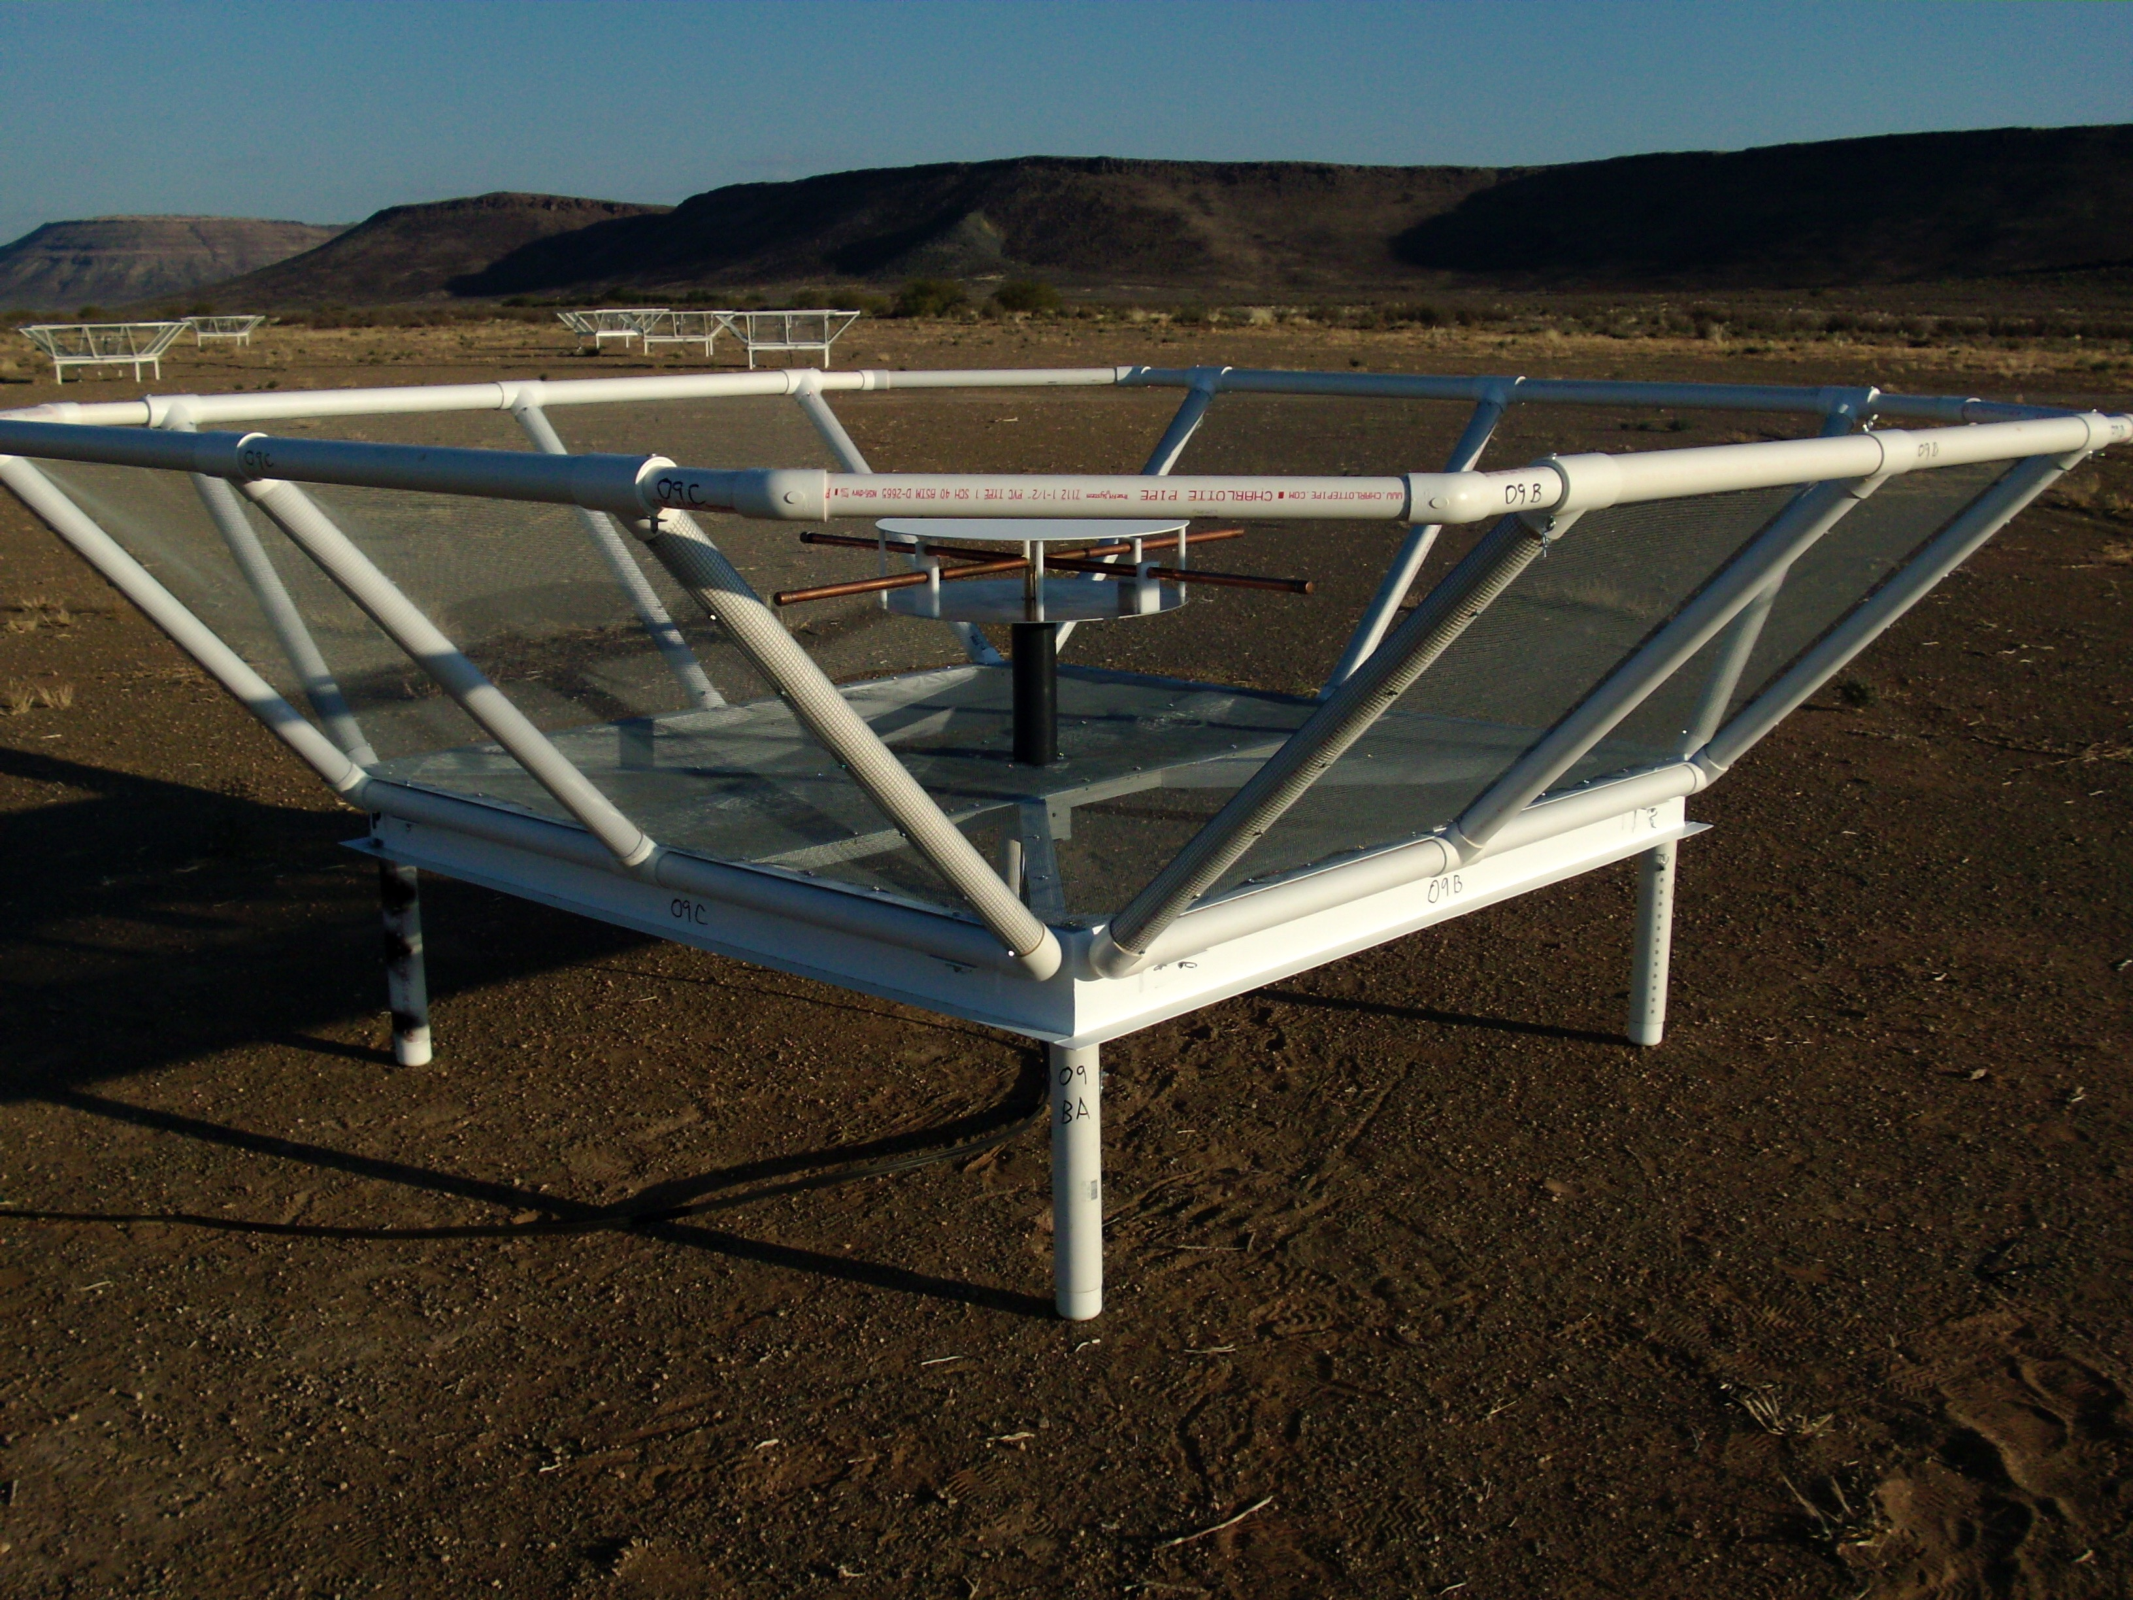
\includegraphics[width=0.9\textwidth]{chapters/instruments/figures/PAPER_dipole.pdf}
\caption{An image of a PAPER dipole element with its groundscreen.}
\label{fig:instruments_PAPER_element}
\end{figure}


Electronics next to the dipole element amplified the voltage by a factor of $10^6$, which then propagated down a 150 foot 75\,$\Omega$ coaxial cable. All cables were of the same length to minimize the amount of extra calibration required per feed, and were above-ground. These cables ran to 8 ``receiverators''; RFI-shielded mini-fridges which contained amplifiers which re-amplified the voltage signals by a factor of $10^4$  (to correct for signal loss along the 150\,ft coaxial cables) and applied an analog bandpass filter. The filter was designed to have a smooth frequency response which was relatively flat between 120 and 180 MHz \citep[e.g.][]{MooreThesis}.

More 50 foot, 75\,$\Omega$ foot coaxial cables ran from these to an RFI-shielded enclosure for further processing. For PAPER and the HERA-19 commissioning array, this enclosure was a specialized shipping container next to the array. For future HERA build-outs, processing will occur in the Karro Array Processing Building (KAPB) and the receiverator architecture will be replaced with underground ``nodes'' (see \citet{deBoer.17} for more detail).

The filtered analog signal was then digitized with a sampling rate of 100 MHz and passed through an F-engine which Fourier transforms the signal using a 4-tap polyphase filter bank (which allowed for a smooth frequency and Fourier-space response; \citet{PricePFB}). The integration time of each Fourier transform was 10\,s. The Fourier transformed signals were distributed over a 10 Gigabit Ethernet switch to the X-engine \citep{Parsons.08}, which cross-multiplied all signals with each other to form visibilities, storing them in {\sc miriad} files.

A summary of the system described above is shown in Figure~\ref{fig:instruments_PAPER_Signal_Chain}.

\begin{figure}
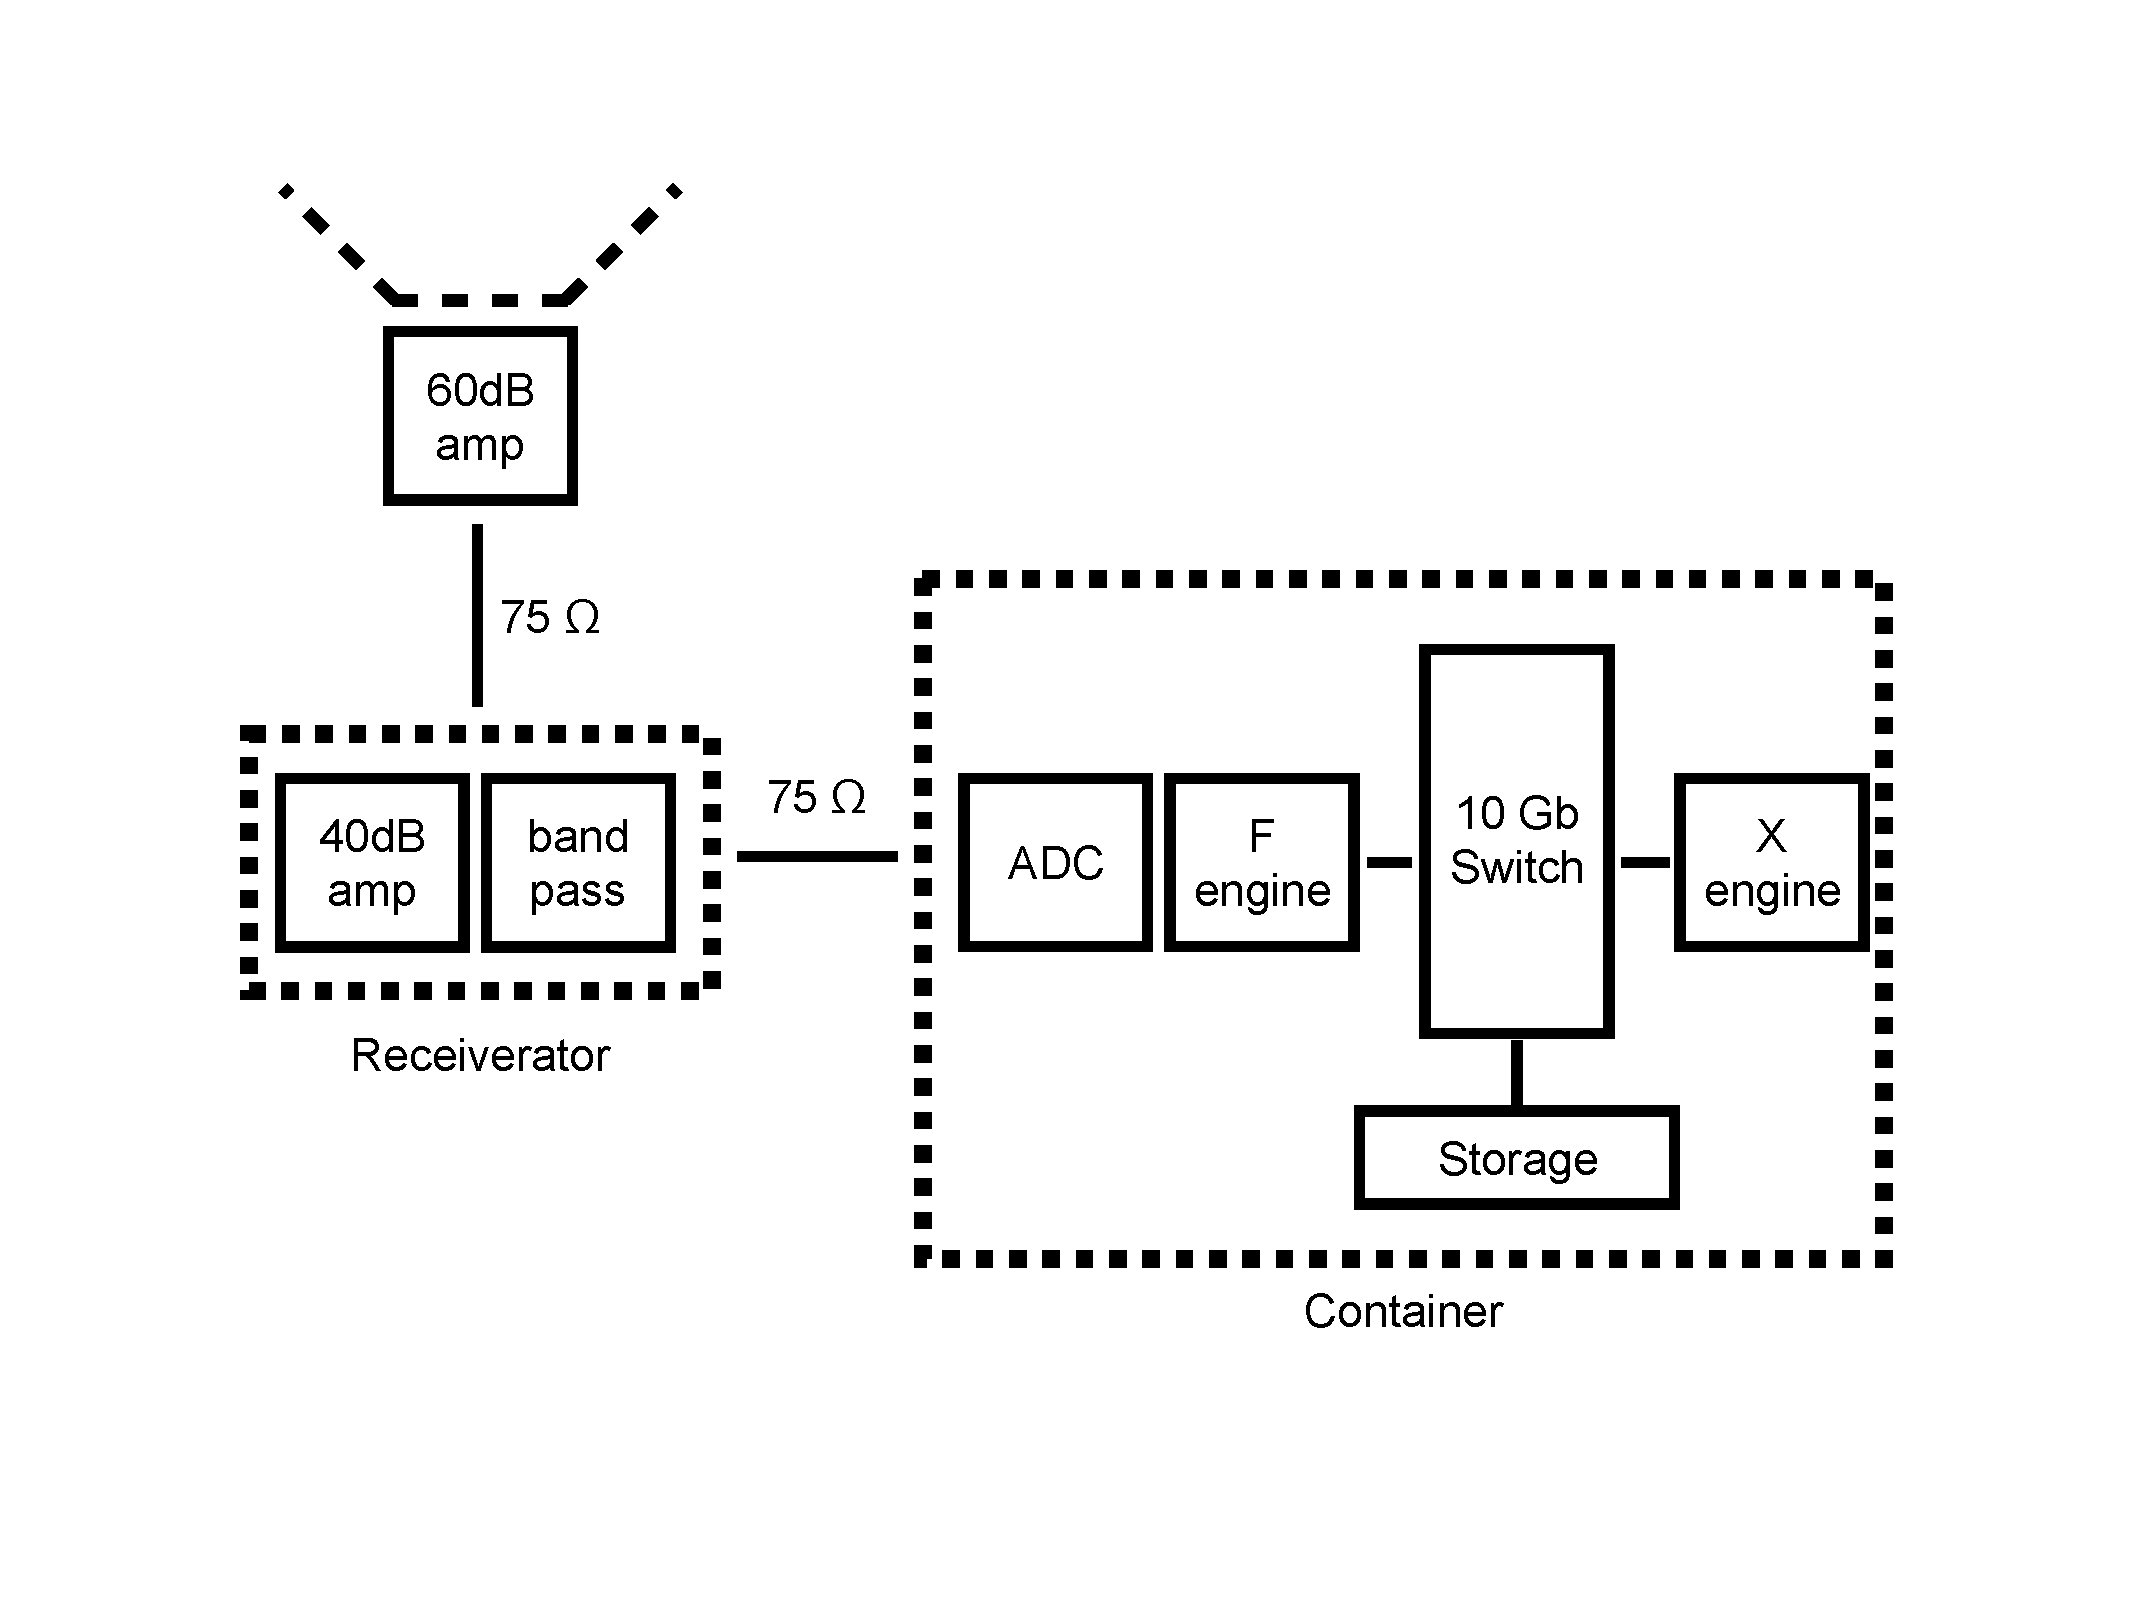
\includegraphics[width=0.9\textwidth]{chapters/instruments/figures/PAPER_system_diagram.pdf}
\caption{A diagram of the PAPER-128 signal chain. Square-dotted lines indicate RFI-shielding.}
\label{fig:instruments_PAPER_Signal_Chain}
\end{figure}

\subsubsection{PAPER-32}

The PAPER-32 array in South Africa used a highly redundant configuration in order to take the measurements resulting in, at the time, the strongest upper limits on the EoR power spectrum \citep[][sections of \citealt{Moore.17} are presented in Chapter~\ref{chapter:ionosphere}]{Parsons.14, Jacobs.15, Moore.17}. The array was in redundant configuration from December 2011 to February 2012. For three nights in September 2011, the 32 elements were reconfigured into an polarized imaging configuration. The results from this deployment were used to make the first 2D power spectra of polarization, presented in \cite{Kohn.16} and in Chapter~\ref{chapter:eor_window_paper32img}. For images and a brief description, see Figure~\ref{fig:instruments_psa32layout}.

\begin{figure}
\centering
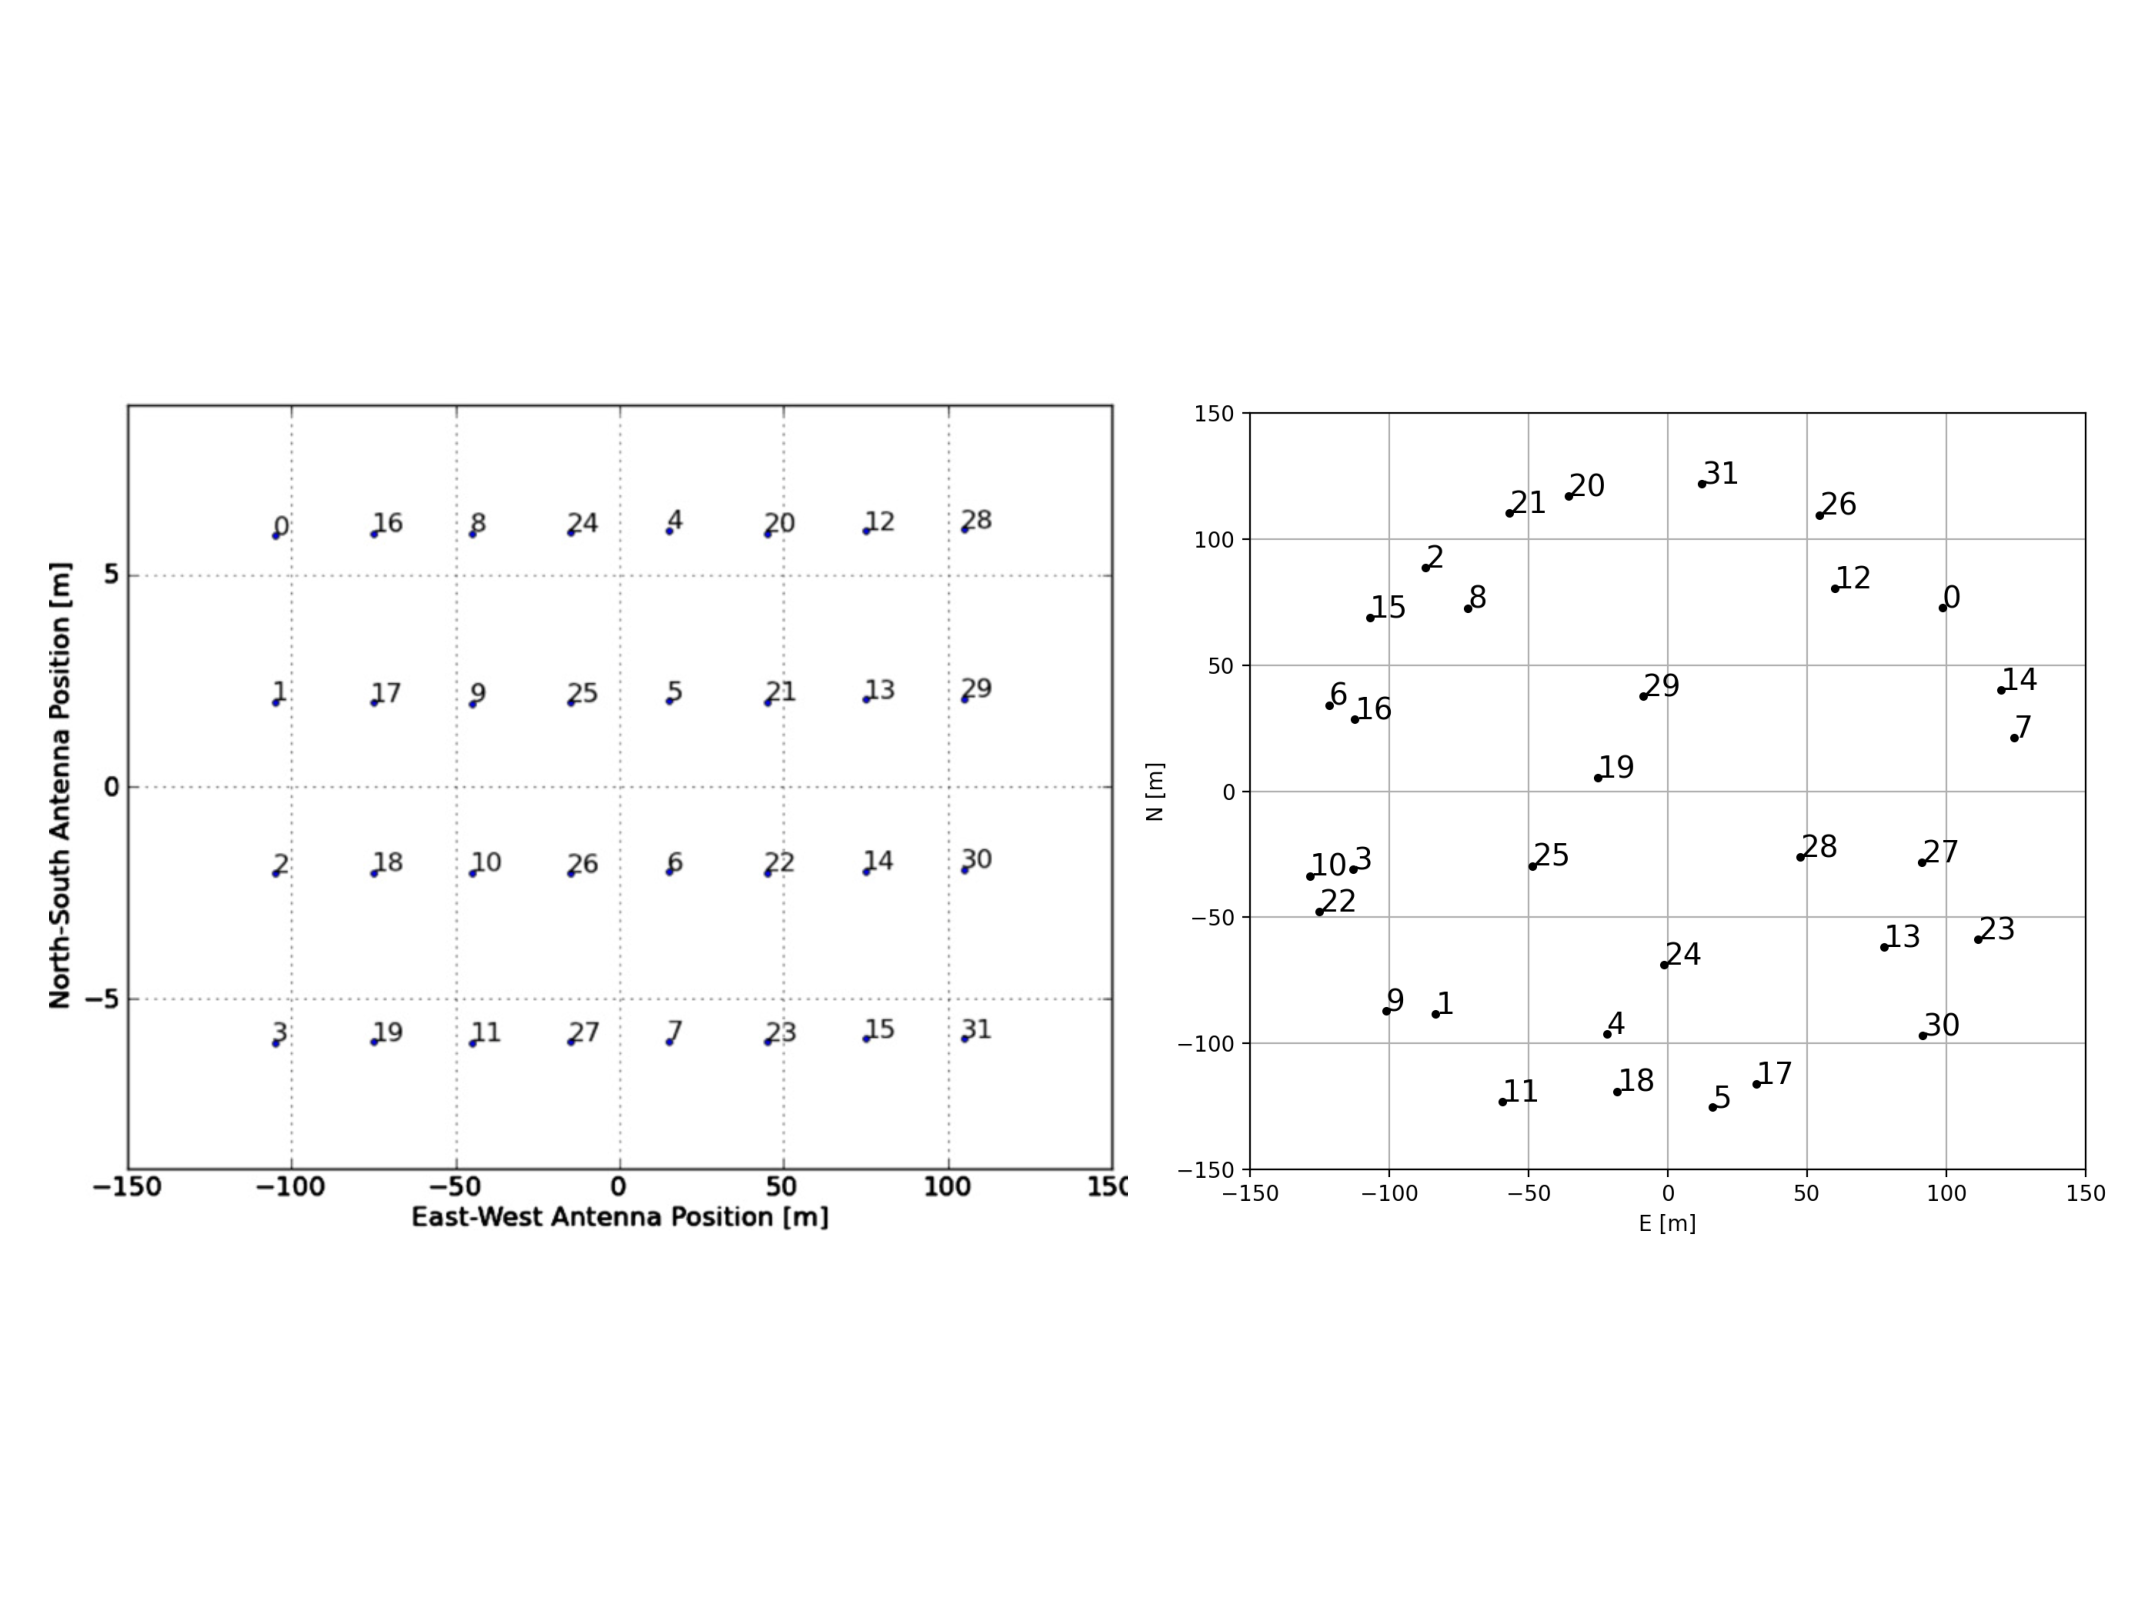
\includegraphics[width=0.9\textwidth]{chapters/instruments/figures/psa32_layouts.pdf}
\caption[The array layouts of the PAPER-32 element deployment in South Africa.]{The array layouts of the PAPER-32 element deployment in South Africa. \textit{Left}: The redundant grid. Four rows, with each element 30\,m from the next in the East-West direction, and closely-packed ($\sim$4\,m) in the North-South direction. Figure taken from \cite{Parsons.14}. \textit{Right}: The polarized imaging array. Elements were arranged in a pseudo-random scatter.}
\label{fig:instruments_psa32layout}
\end{figure}

\subsubsection{PAPER-64}

During the PAPER-32 EoR integration, there were actually 64 antennas present in the Karoo, South Africa. However, the correlator at that time could only process 64 voltage streams -- enough for 32 dual-polarization antennae. This is why 64 element single-instrument-polarization imaging results were published prior to any PAPER-32 studies \citep{Jacobs.13, Stefan.13}. EoR integrations in the 64 element redundant configuration were only possible after a new correlator was produced in 2012. Results from this array were published in \cite[][{\color{red}Cheng et al. \textit{in prep.}, Kolopanis et al. \textit{in prep.}}]{Ali.15, Pober.15}. The array layouts are shown in Figure~\ref{fig:instruments_psa64layout}.

\begin{figure}
\centering
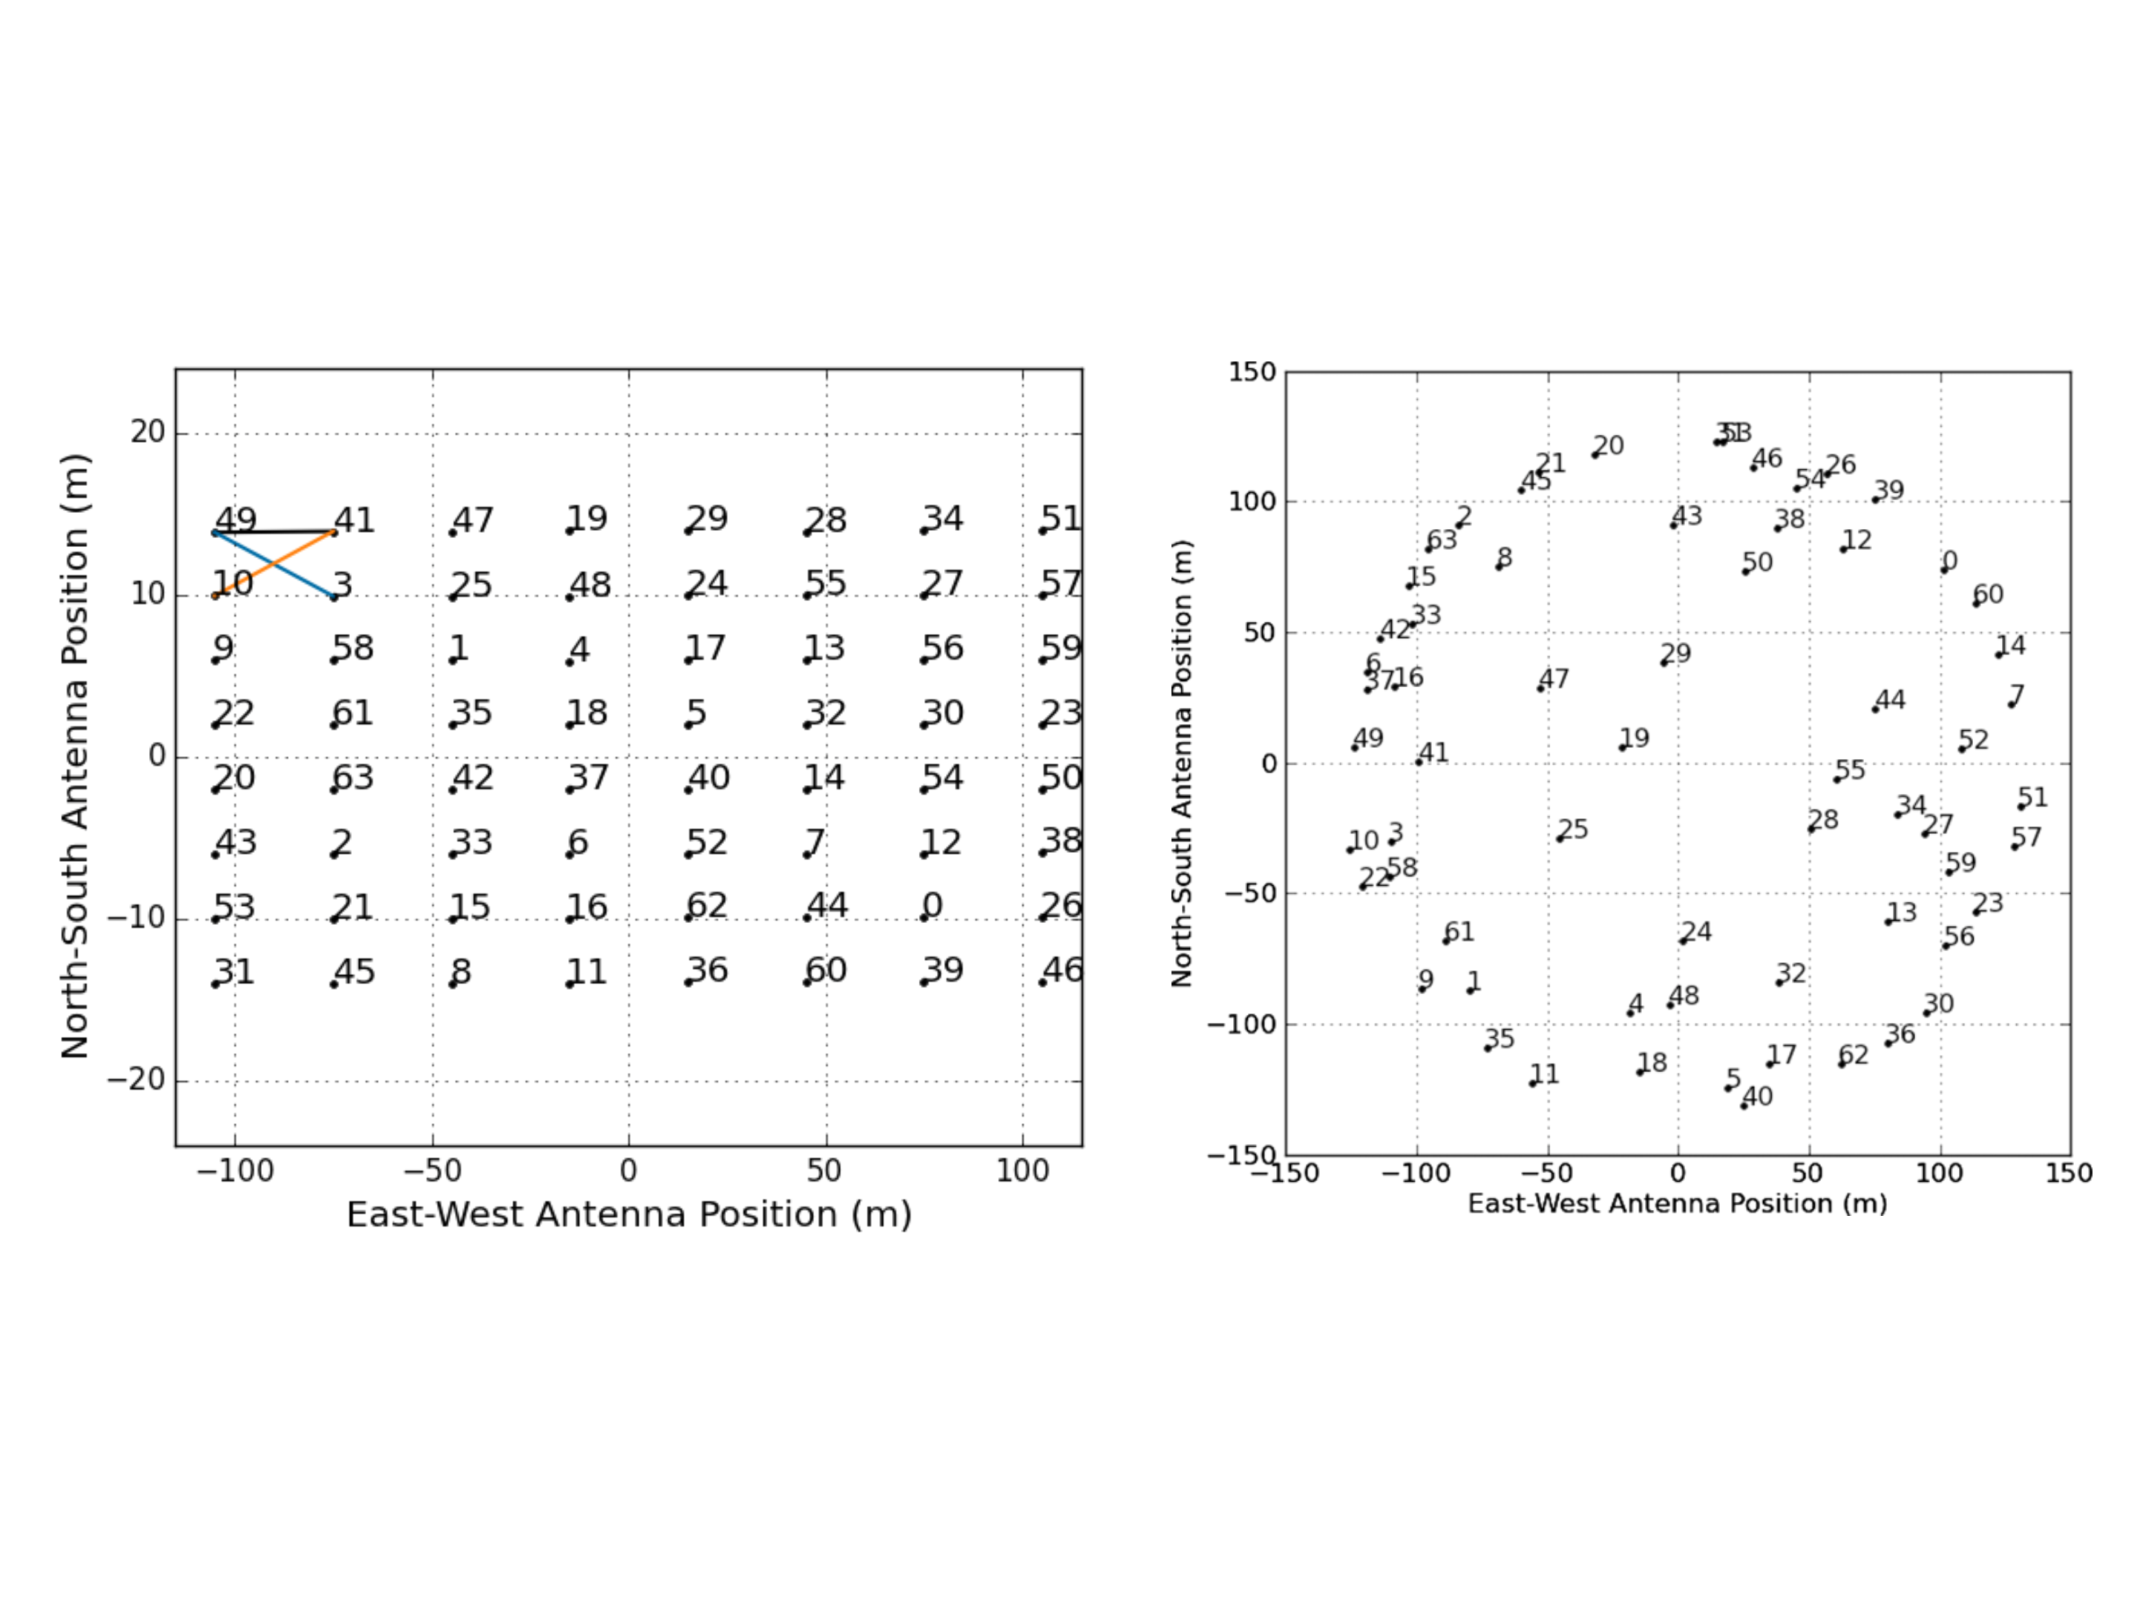
\includegraphics[width=0.9\textwidth]{chapters/instruments/figures/psa64_layouts.pdf}
\caption[The array layouts of the PAPER-64 deployment.]{The array layouts of the PAPER-64 deployment. \textit{Left}: The redundant grid, built-out from the PAPER-32 grid. Figure taken from \cite{Ali.15}, which highlights the baseline-types used for power spectrum measurements. \textit{Right}: the imaging array, used by \cite{Jacobs.13} to set an absolute flux scale for PAPER experiments. Figure taken from \cite{Jacobs.13}.}
\label{fig:instruments_psa64layout}
\end{figure}

\subsubsection{PAPER-128}

The culmination of the PAPER experiment was the 128 element deployment. There were two observing seasons recorded: November 2013 to March 2014, and July 2014 to January 2015. In this configuration, 112 antennas were laid-out in a redundant grid with 15\,m East-West spacings and 4\,m North-South spacings. The remaining 16 antennas were arranged in `out-rigger' and `in-rigger' positions to increase \textit{uv}-coverage and enable some level of imaging. Results from the first observing season of this array are presented in Chapters~\ref{chapter:data_prep_and_proc}, \ref{chapter:polcal} and \ref{chapter:eor_window_psa128}. The array layout is shown in Figure~\ref{fig:instruments_psa128}.

\begin{figure}
\centering
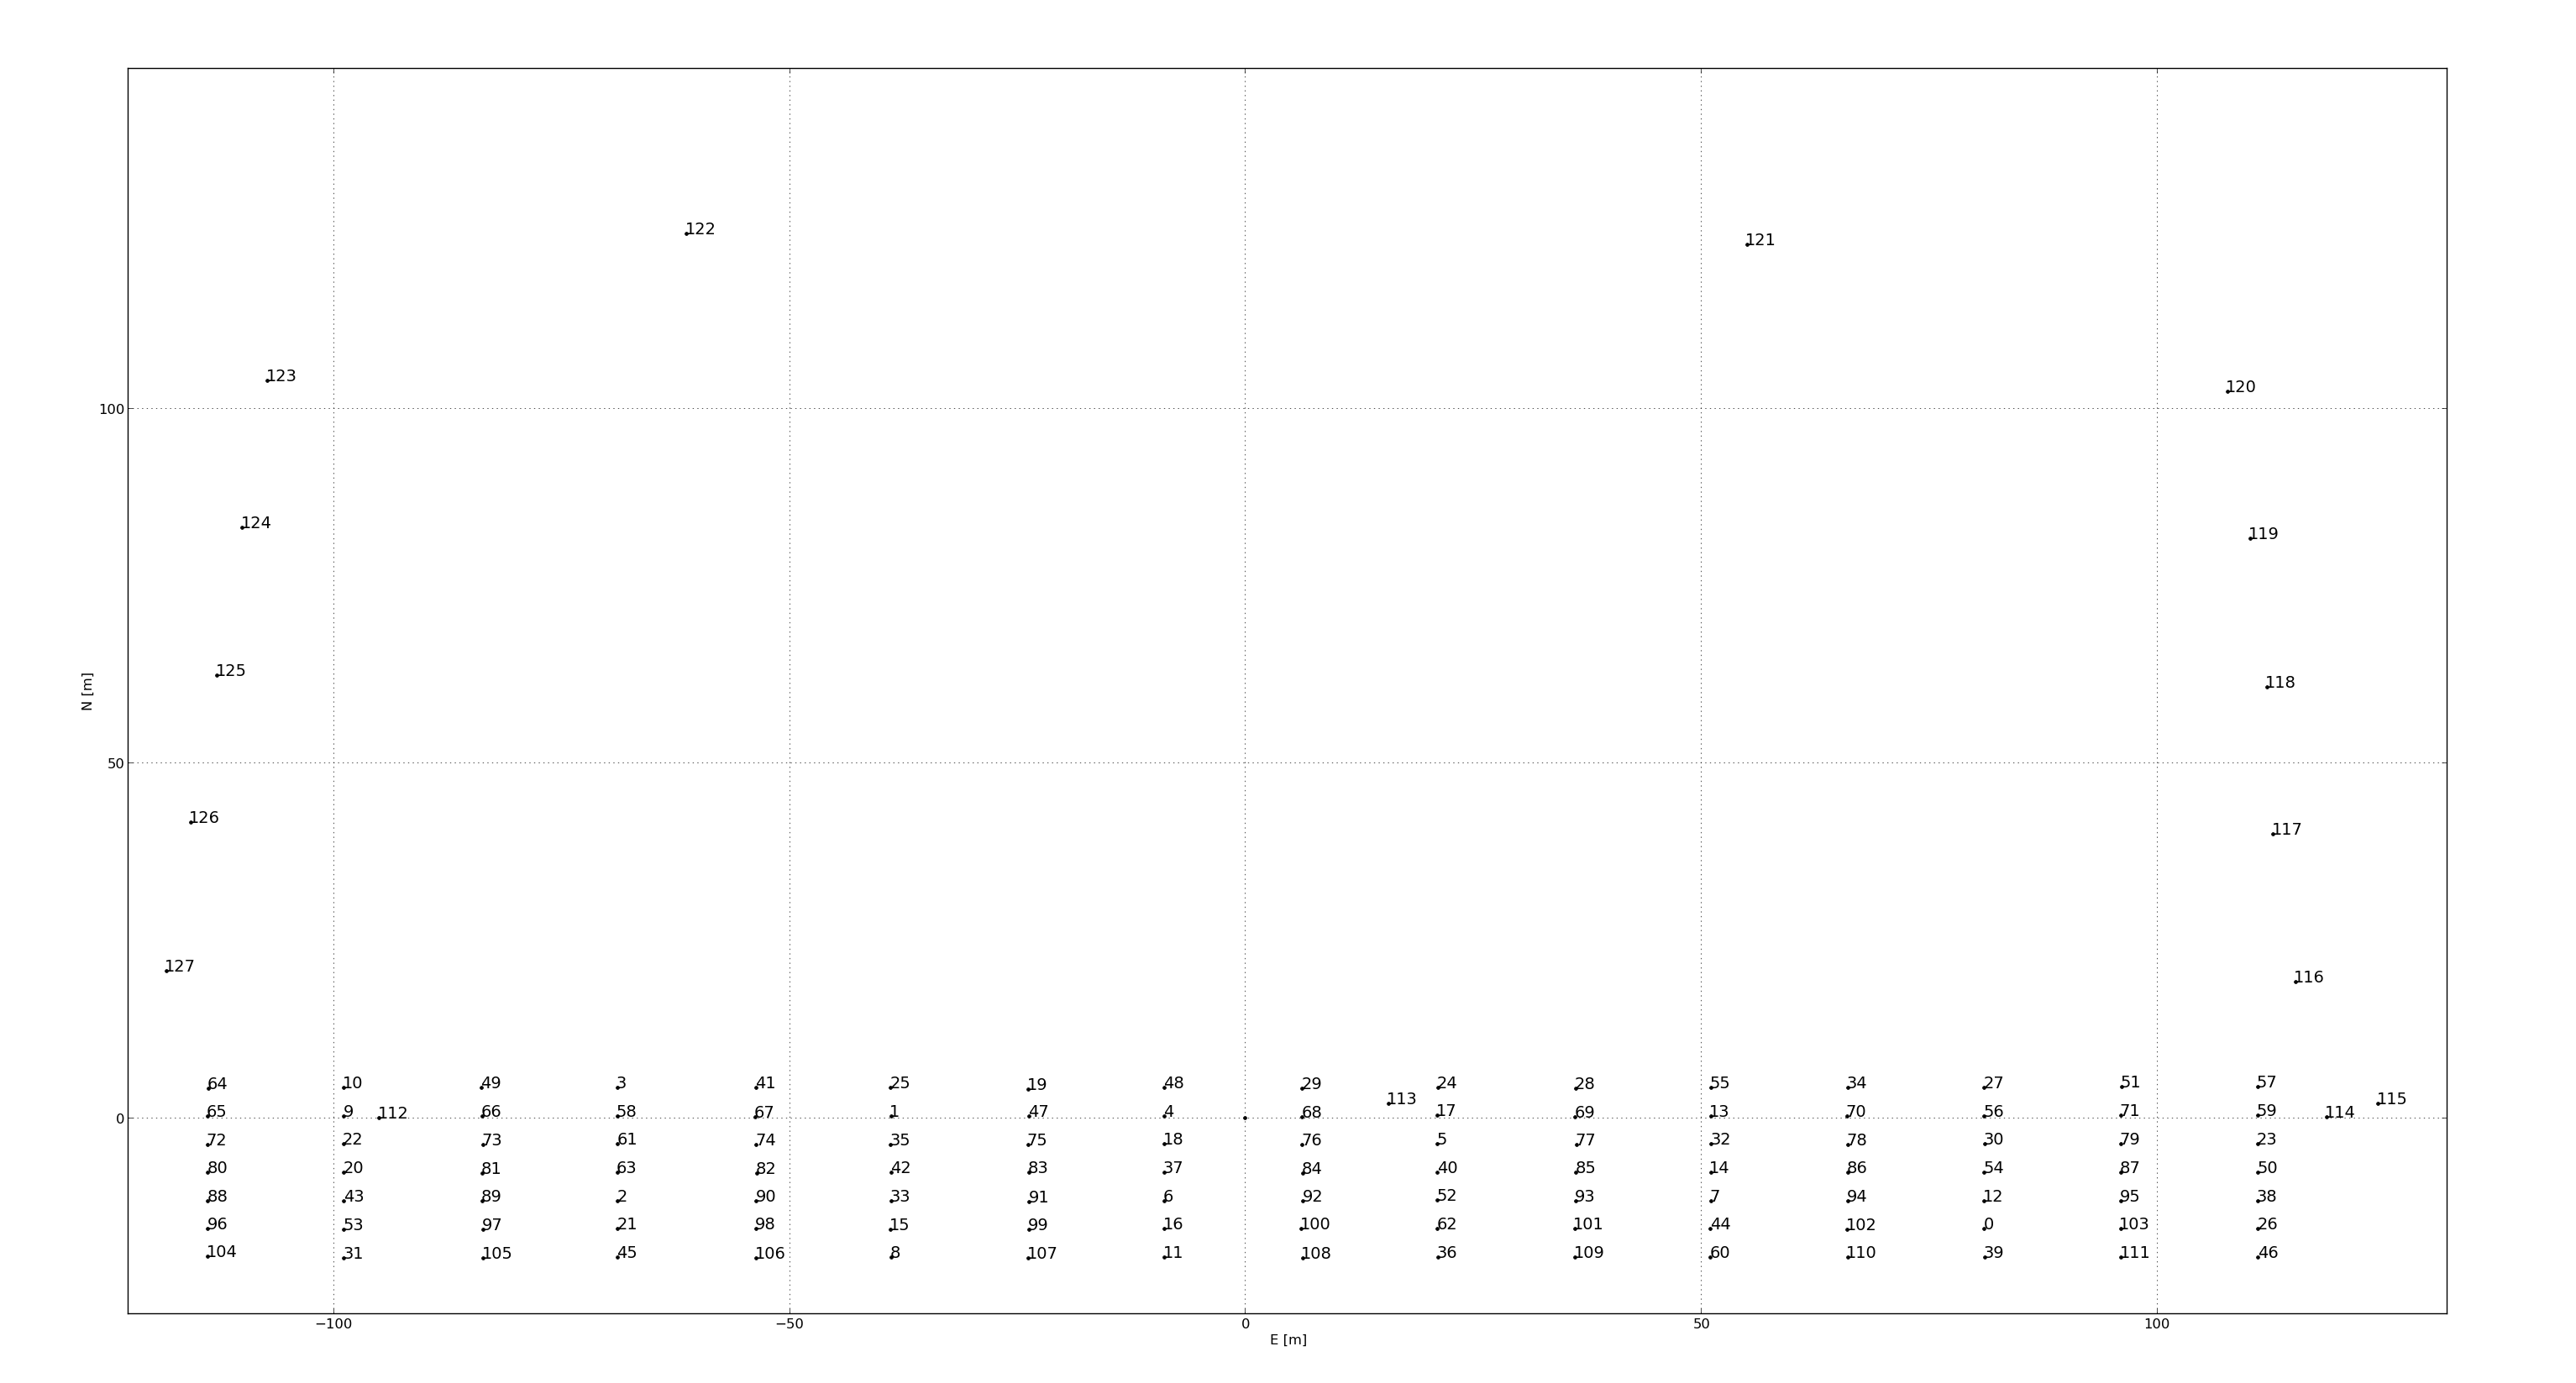
\includegraphics[width=0.9\textwidth]{chapters/instruments/figures/antlayout_psa128.png}
\caption[The PAPER-128 array layout.]{The PAPER-128 array layout. 112 antennas were laid-out in a redundant grid with 15\,m East-West spacings and 4\,m North-South spacings, and the remaining 16 antennas were arranged in `out-rigger' and `in-rigger' positions to increase \textit{uv}-coverage.}
\label{fig:instruments_psa128}
\end{figure}

\subsection{The Hydrogen Epoch of Reionization Array (HERA)}
\label{subsec:hera_instrument}

HERA was ranked as the ``top priority in the Radio, Millimeter, and Sub-millimeter category of recommended new facilities for mid-scale funding'' by the National Research Council Decadal Survey in astronomy and astrophysics \citep{Astro2010}. It brought together the largely US-based experts working on PAPER and the MWA to construct a new low-frequency array on the PAPER site in South Africa. The array, comprised of 14\,m diameter dishes, was designed to be build-out in stages of close-packed hexagons of increasing size. For a full description of the instrument, refer to \cite{deBoer.17}.

The design of the HERA dish, feed, antenna layout and signal chain are intimately related to lessons learned by the PAPER and MWA EoR teams about the nature of EoR measurements \citep[e.g.][]{Nithya.15a}. One of the major considerations was how the instrument couples to the bright foregrounds, and how to control that coupling -- the paradigm of the ``wedge'' and the ``EoR Window'', which are discussed in detail in Chapter~\ref{chapter:eor_window_theory}. Measurements based on prototype feeds were presented in \cite[][Patra et al. \textit{submitted}]{Ewall-Wice.16.HERA_Dish, Neben.16}.

HERA is a staged experiment, building-out in close-packed hexagons from a 19 element commissioning array, to 37, 127, 240 and finally 350 elements (320 in a dense, fractured core and 30 out-riggers, see \citealt{Dillon.16} for more detail). Figure~\ref{fig:instruments_hera_layout} shows a rendering of the core alongside an image of the HERA-19 commissioning array.

\begin{figure}
\centering
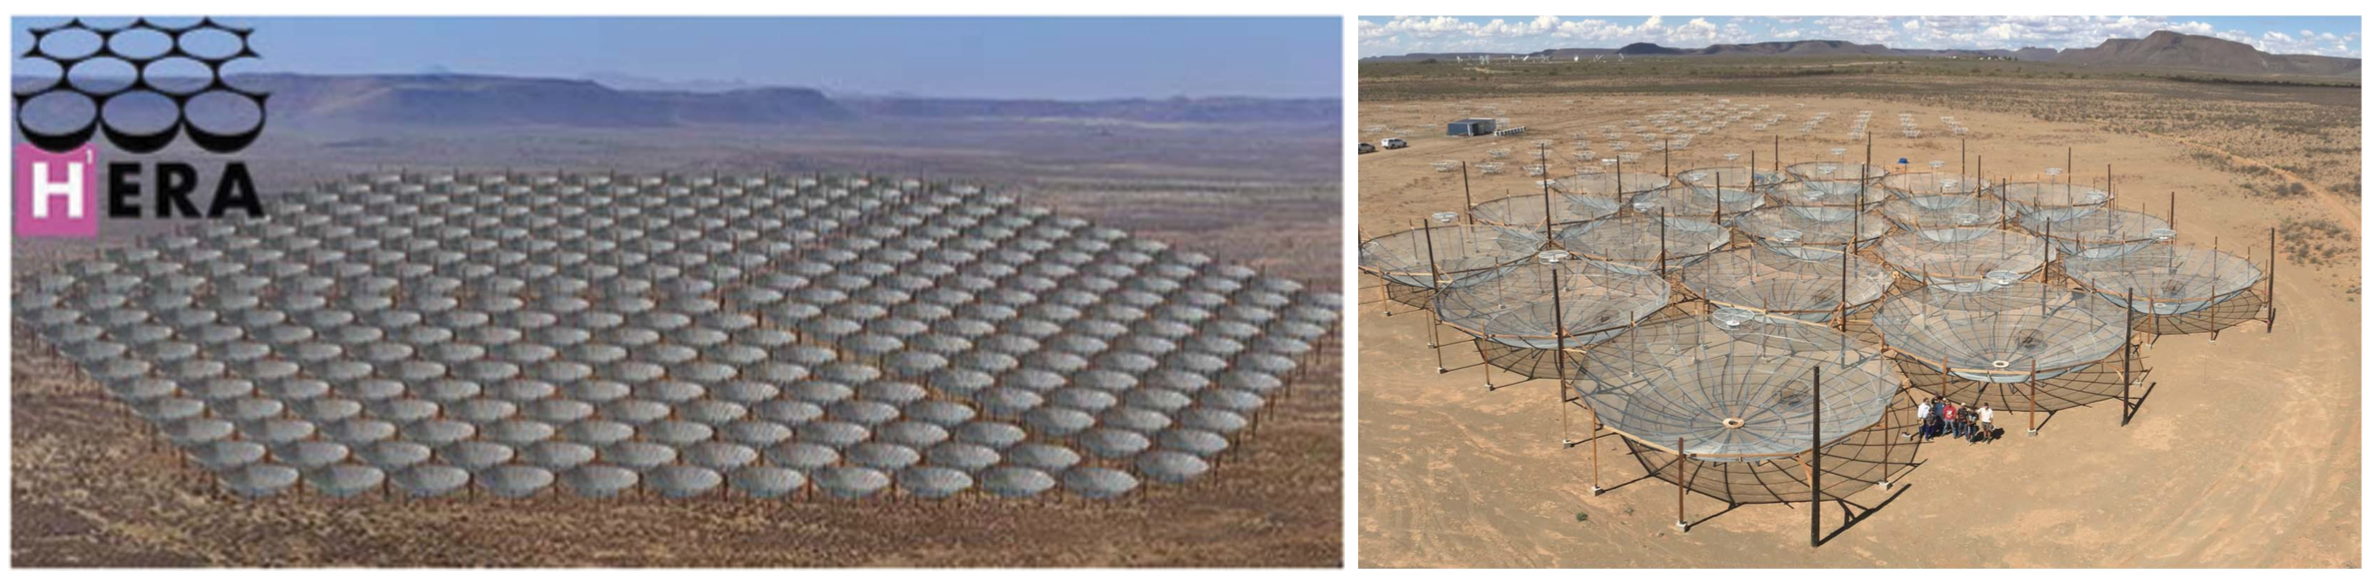
\includegraphics[width=0.9\textwidth]{chapters/instruments/figures/HERAlayout_deBoer.png}
\caption[Future vision and physical commissioning HERA layout.]{\textit{Left}: a rendering of the 320 element HERA core. \textit{Right}: the 19 element commissioning array (with the construction team). Leftover PAPER dipoles can also be seen in the background, forming three experimental arrays (described in Section~\ref{subsubsec:instruments_hera19}). Figure taken from \cite{deBoer.17}.}
\label{fig:instruments_hera_layout}
\end{figure}

\subsubsection{HERA-19 Commissioning Array}
\label{subsubsec:instruments_hera19}

In October 2015 a HERA commissioning array was completed, connected to the PAPER-128 256-input correlator. This array comprised of four separate components: the first 19 HERA dishes in a close-packed hexagon (HERA-19), 19 PAPER dipoles at the central locations of a hexagon of future HERA dishes (the ``PAPER-Hex''), 40 PAPER dipoles in a redundant grid where every-other dipole was rotated 45$^{\circ}$ (to experiment with different polarization bases; ``PAPER Pol''), and the remaining inputs filled with PAPER dipoles arranged in a pseudo-random scatter for imaging (``PAPER-Img''). Studies with this array are presented in Chapter~\ref{chapter:data_prep_and_proc} and \ref{chapter:eor_window_HERA}. A diagram of the commissioning setup is shown in Figure~\ref{fig:instruments_hera19_layout}.

\begin{figure}
\centering
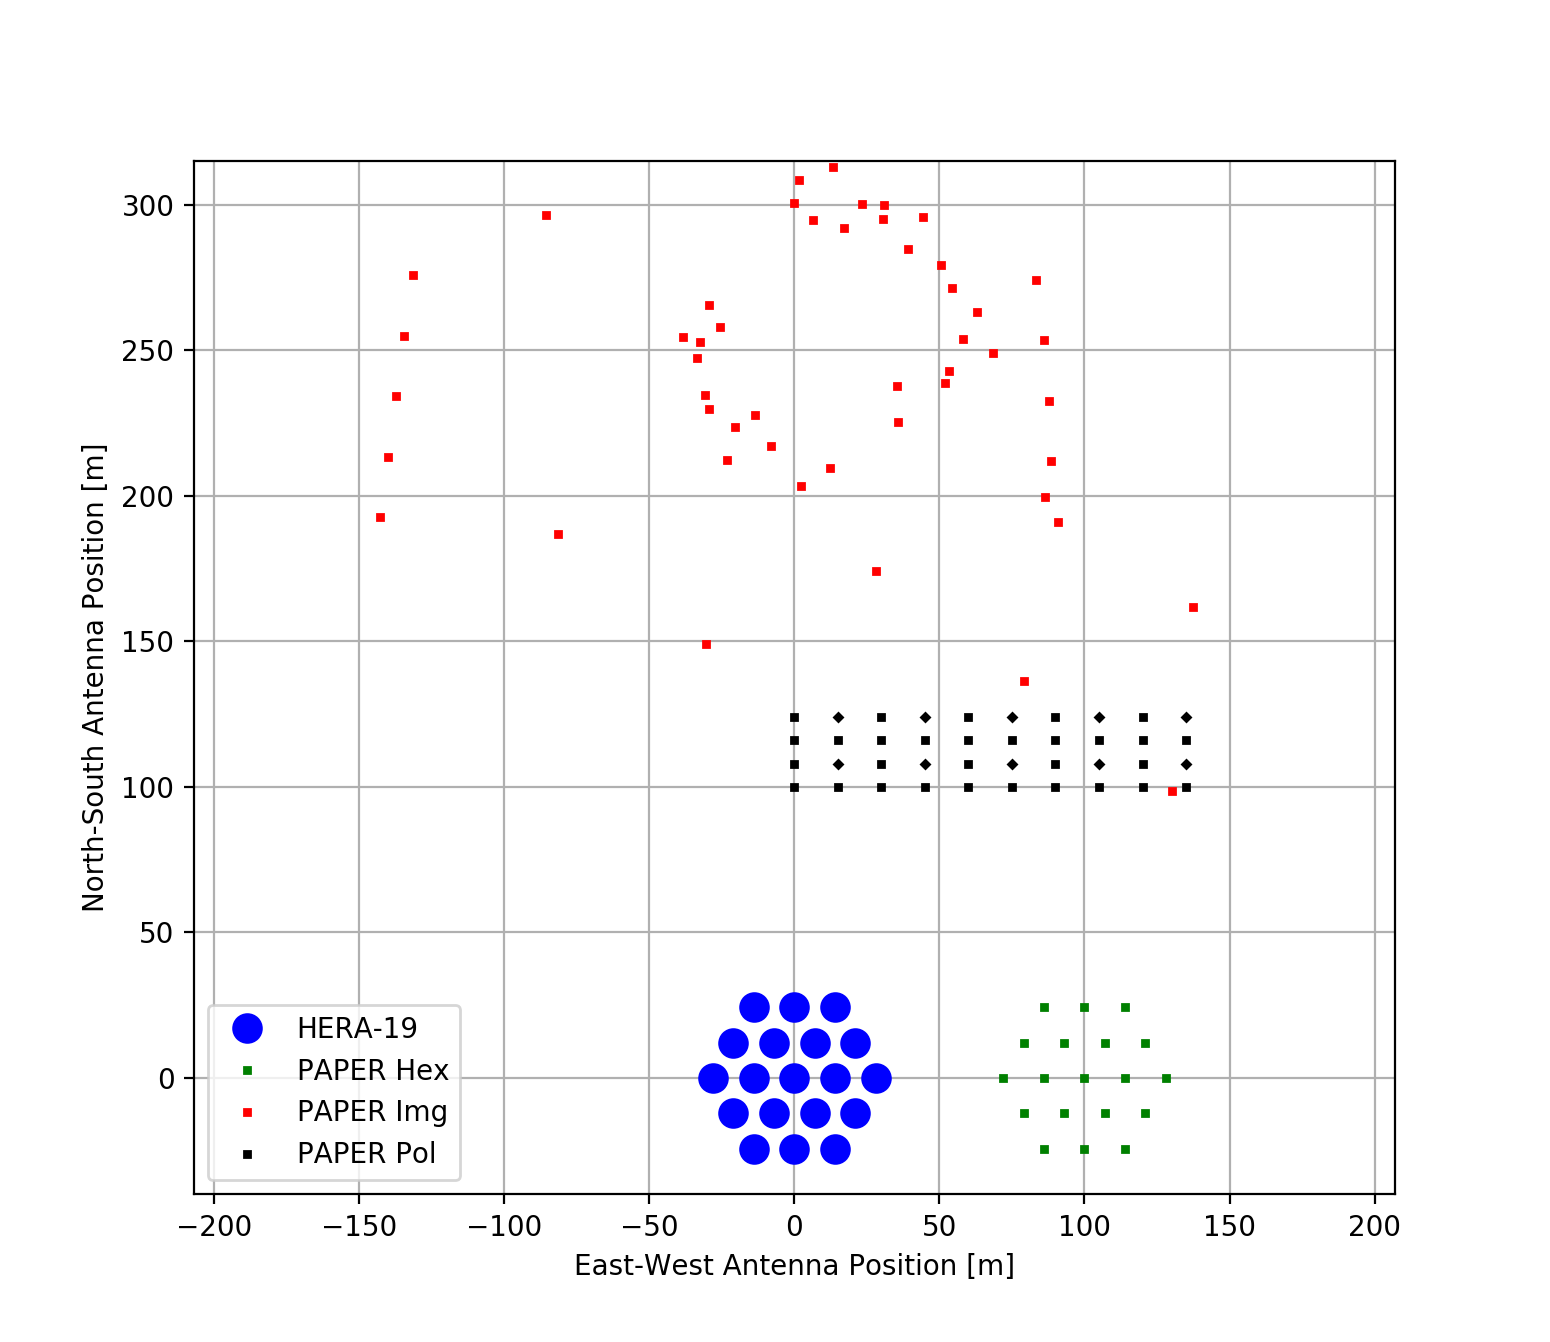
\includegraphics[width=0.9\textwidth]{chapters/instruments/figures/h19layout.png}
\caption{Positions of antennae in the HERA-19 Commissioning Array (including the experimental ``subarrays'').}
\label{fig:instruments_hera19_layout}
\end{figure}

\subsubsection{Future HERA Build-Outs}

Each HERA element is much more sensitive than a PAPER element, based purely on collecting area. Figure~\ref{fig:instruments_sensitivity} illustrates the varying sensitivities and collecting areas of different arrays and their elements, respectively. PAPER-128 was forecast to make marginal detections of the EoR power spectrum after $\sim$1000 hours of integration -- HERA-127 should be capable of characterizing the EoR power spectrum at high significance, and the full HERA-350 array will be an extremely powerful survey instrument \citep[e.g.][]{PoberMemo}. We present forecasts for this future instrument in Chapter~\ref{chapter:ksz_21cm}.

\begin{figure}
\centering
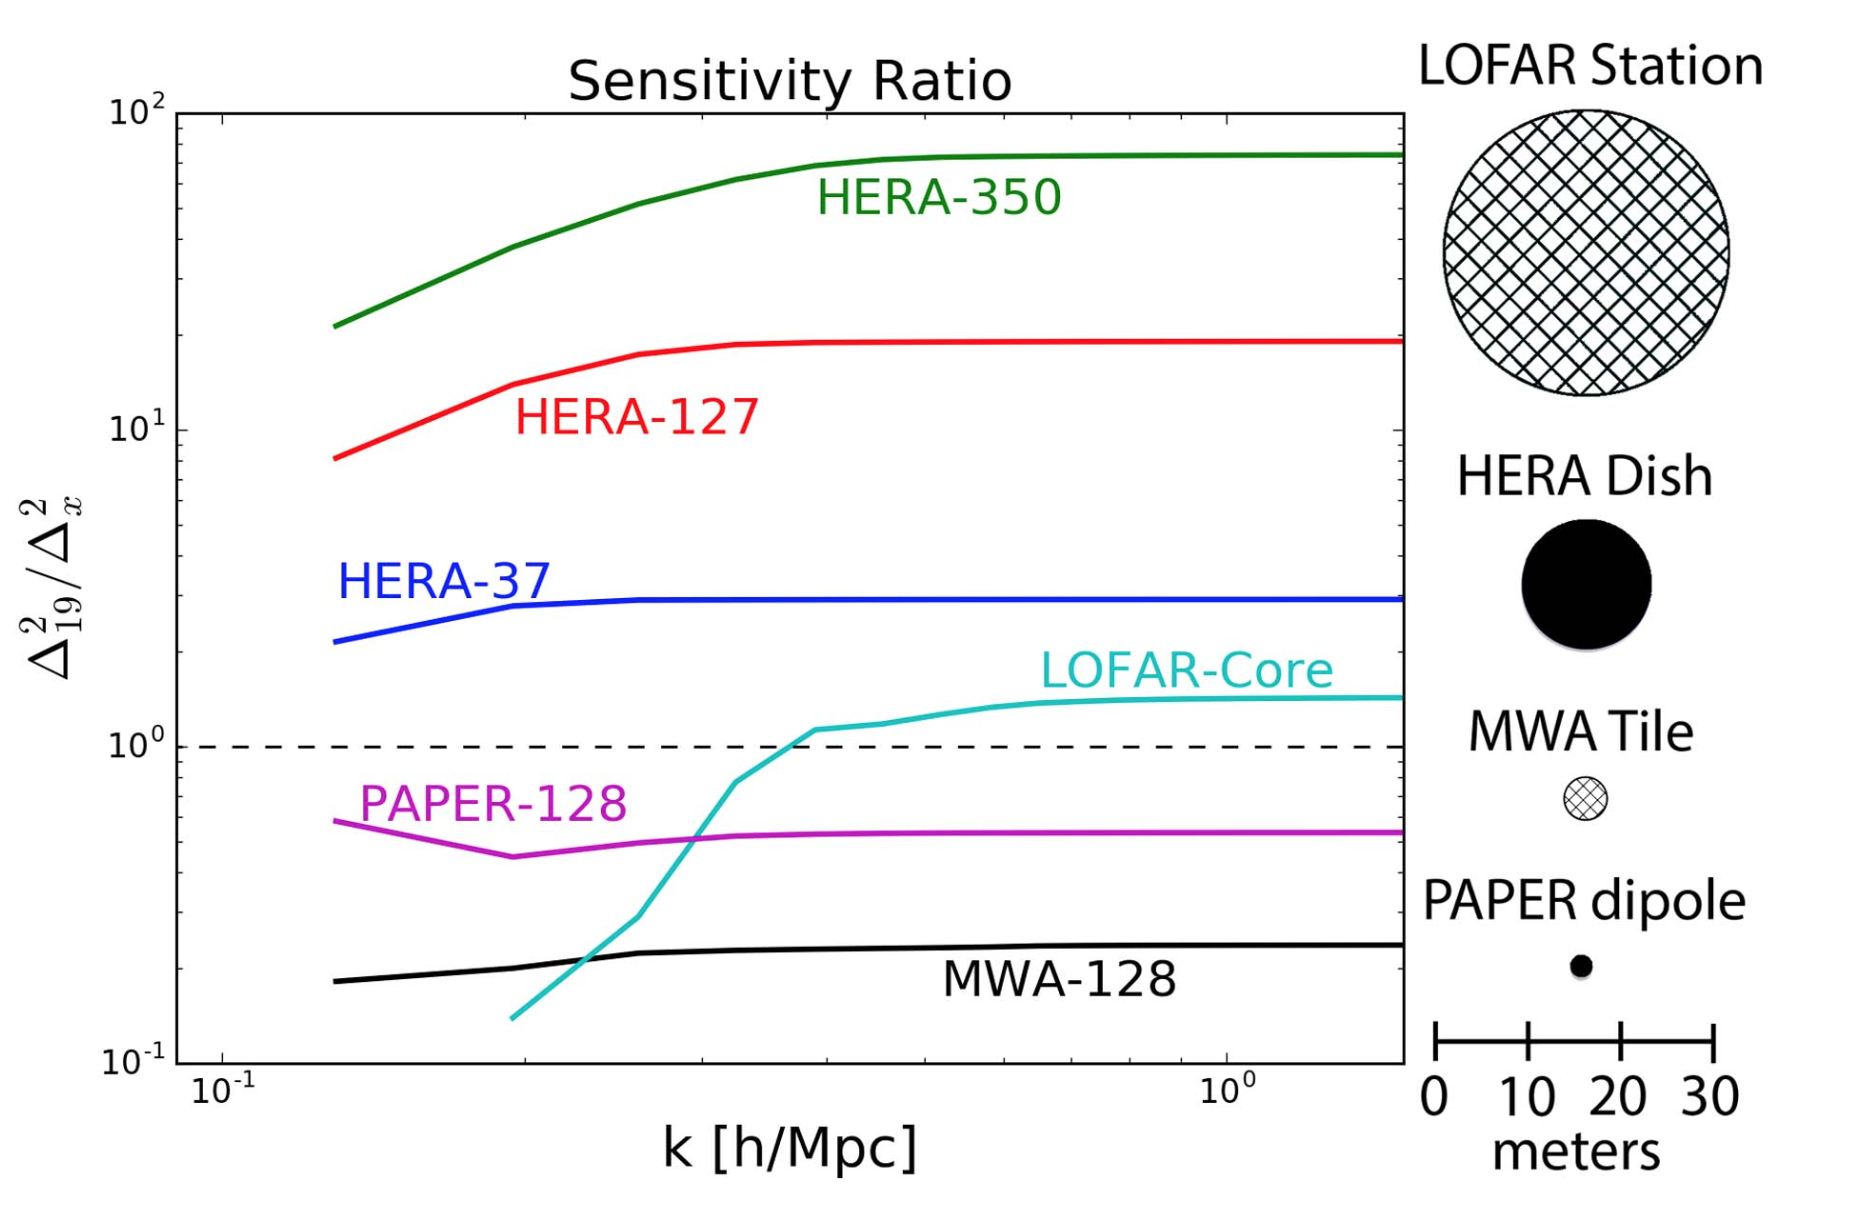
\includegraphics[width=0.9\textwidth]{chapters/instruments/figures/deBoer_sensitivities.png}
\caption[Array sensitivity as a function of \textit{k}-mode relative to HERA-19]{Instantaneous array Sensitivities as a function of \textit{k}-mode (e.g. Chapter~\ref{chapter:eor_window_theory}) relative to HERA-19. Differing element collecting areas are shown on the right. Taken from \cite{deBoer.17}.}
\label{fig:instruments_sensitivity}
\end{figure}

\section{Other current and future interferometers}
\label{sec:not_used_in_this_work}

PAPER and HERA were not the only instruments researching the EoR and how to detect it. Several low-frequency interferometers around the world are contributing to the understanding of the EoR and the difficulties of observing it. Below I briefly describe a few of the leaders of the field -- but it is not an exhaustive list.

\subsection{The Low Frequency Array (LOFAR)}

The LOw Frequency ARray (LOFAR) is an interferometer made-up of ``stations'', the core of which are arranged in a random scatter near Exloo in the Netherlands \citep{vanHaarlem.13}. LOFAR baselines extend across Europe with stations in Ireland, Sweden, Germany, Poland and other locations. These extremely long baselines can provide LOFAR with exquisite imaging capabilities. 

LOFAR has detected diffuse, linear polarization structures that may be related to the Milky Way's magnetic field and interstellar medium \citep{Jelic.15}. \cite{Patil.17} presented deep limits on the EoR power spectrum from one night of LOFAR data (also see \citet{Yatawatta.13}). A series of publications has investigated polarization in Fourier space \citep{Jelic.14, Asad.15, Asad.16, Asad.17} -- results that we build upon and verify throughout this work.

\subsection{The Murchinson Widefield Array (MWA)}
\label{subsec:mwa_instrument}

The Murchinson Widefield Array (MWA), based in Murchison Radio-astronomy Observatory in Western Australia, is composed of 256 `tiles' of 16 feeds each. At the time of writing, 72 tiles are arranged in compact hexagonal configurations in an effort to increase EoR sensitivity while retaining imaging capabilities with the rest of the array. The most complete low-frequency catalog of the southern sky, GLEAM, was presented by \cite{Hurley-Walker.17}.

The MWA uses separate analysis pipelines for its EoR measurements \citep{Sullivan.12, Jacobs.16, Trott.16}, an concept that will be implemented on future HERA measurements. The MWA has detected polarized signal from diffuse Galactic emission \citep{Lenc.16, Lenc.17} and set deep limits on the EoR power spectrum \citep[e.g.][]{Dillon.14, Dillon.15}. Pioneering work on the ionosphere was accomplished using MWA data \citep[e.g.][]{Loi.15}, which we discuss in Chapter~\ref{chapter:ionosphere}.

\subsection{Square Kilometer Array -- Low band (SKA-Low)}
\label{subsec:skalow_instrument}

The Square Kilometer Array (SKA) will be built on two sites: the Karoo Radio Quiet Zone, currently occupied by HERA, will be the central location of the ``high--mid band'' (350 MHz -- 14 GHz; ``SKA-Mid'') observatory and the Murchinson Radio-astronomy Observatory, currently occupied by the MWA, will be the central location of the ``low band'' observatory (50 -- 350 MHz; ``SKA-Low'').

SKA-Low will consist of over 100,000 receiving elements in an imaging configuration. It will be the most powerful low-frequency radio telescope ever created, and be used not only for EoR science but a host of low-frequency science objectives \citep[e.g.][]{SKABook, Schilizzi.07, Dewdney.09}. Learning from the work of EoR teams working on PAPER, HERA, MWA, LOFAR and other instruments will be crucial to the success of SKA-Low's EoR science goals.

%
% brief overview of instruments used in this work:
%   PAPER: 32, 32-pol-img, 64 (xtlak), 128
%   HERA: 19, H1C?
%% make sure to mention signal chain -- X; F engines
% instruments of note, not used in this work, but exploring similar things and facing similar challenges:
%   LOFAR, MWA
%   SKA-Low
%
\part{Structure in Fourier space}
\chapter{Peering through the EoR Window}
\label{chapter:eor_window_theory}

Chapter~\ref{chapter:eor_intro} argued the promise of direct observations of {\sc hi} during the EoR. A direct detection has not yet been made, largely due to the overwhelming power of foregrounds compared to the target signal. As shown in Chapter~\ref{chapter:astro_rad}, foreground radiation is a factor of roughly $10^4 -- 10^5$ times brighter than predicted 21\,cm anisotropies .  In the past decade, however, enormous improvements have been made in understanding how to decontaminate interferometric visibilities, and excavate the target signal. The leverage astronomers have to use is the exceptional smoothness of low-frequency synchrotron radiation, the dominant foreground emission mechanism. In this Chapter, I review the `Foreground Wedge \& EoR Window' paradigm used to delineate foreground power from noise and {\sc hi} emission. In Section~\ref{sec:eor_window_foreground_wedge} I introduce the concept of the foreground wedge, and methods used by astronomers to take advantage of it: either avoiding it, or subtracting it. In Section~\ref{sec:eor_window_problem_of_pol}, I make plain how astrophysical and instrumental polarization complicates this picture.

\section{The foreground wedge \& the EoR window}  % ugh I don't like this section title
\label{sec:eor_window_foreground_wedge}

Mitigation of foregrounds is essential for accessing the EoR. This fact was recognized by \cite{Madau.97} in one of the first in-depth studies of the promises and challenges of 21\,cm tomography. To overcome foreground radiation, they suggested that fitting the synchrotron spectra, relying on its smoothness, may have been sufficiently accurate to subtract the foregrounds from the total signal.
However, for the next two-or-so decades, there were few low-frequency instruments powerful and well-characterized enough to attempt an EoR detection, and precise observations of low-frequency foregrounds did not exist. The first work to concentrate solely on the foreground challenge was \cite{DiMatteo.02}. Their outlook was pessimistic, but they suggested the challenge was surmountable with sufficiently accurate and precise multi-frequency fitting. \cite{Peng.03} were among the first to point out that interferometers are inherently chromatic, and therefore the instrument itself must be taken in to account when considering the frequency dependence of EoR foregrounds.

\cite{Wang.06}, while theoretically pursuing optimal methods of frequency cleaning, were among the first to discover the advantages of describing the foregrounds statistically in Fourier space. In their numerical simulations they recognized that visibilities, for single baselines, dominated by smooth synchrotron foregrounds could be Fourier transformed along their frequency axis and mapped in to a relatively narrow range of Fourier space. If the visibilities also contained spectrally-structured EoR and noise models, these required many more Fourier modes for their description. With sufficient bandwidth and frequency resolution, one would be able to delineate a boundary between these regions of Fourier space.

% Datta = coined term "wedge" and "window". "Discovered" the wedge -- more than one baseline!
% Parsons 2012b => delay spectrum, provided explanation
% explanation has been continually refined (Morales 12, Vedantham 12, Hazelton 13, Pober 13, Thyagarajan 2013, Trott 14, Liu 14a,b)
% Nithya => importance of instrument, beam => strategies per instrument

% foreground wedge and EoR window -- Nithya predictions -- importance of beam

\subsection{Foreground avoidance}
% Foreground avoidence: delay spectrum; basic PAPER and HERA results (including Kohn et al. 2016, 2018)
\subsubsection{Power spectra}
% Define power spectra in the delay paradigm
% X and Y factors
\subsubsection{Noise spectra}
% define noise spectrum

\subsection{Foreground subtraction}
% Foreground subtraction: theory and LOFAR results
% they need to subtract because they have almost no window

\subsection{Hybrid methods}
% Hybrid approach: MWA

\section{The Problem of Polarization}
\label{sec:eor_window_problem_of_pol}
% polarization in wedge space -- my nice freq vs fourier space diagram? -- basically everything from Moore 2013


% for the rest of this Part...
In this Part, I have recorded my efforts to reduce interferometric observations from PAPER and HERA, taking as much care as possible to avoid introducing spectral structure to the visibilities. My work has centered around the problem of polarization in the EoR window paradigm. In the following Chapters, I discuss quality assurance metrics and data compression (Chapter~\ref{chapter:data_prep_and_proc}), polarized calibration (Chapter~\ref{chapter:polcal}), the effect of the ionosphere on polarized power spectra (Chapter~\ref{chapter:ionosphere}), and three successively deeper integrations on polarized power, concentrating on successively thinner slices of $k_{\perp}$ (Chapters~\ref{chapter:eor_window_paper32img} -- \ref{chapter:eor_window_psa128}).
%
% -- sort of a lit review chapter --
% The issue of low frequency foregrounds for EoR measurements
% Define power spectra...
% foreground wedge and EoR window
% Foreground avoidence: delay spectrum
% Foreground subtraction: theory and LOFAR results
% Hybrid approach: MWA
% polarization in wedge space -- my nice freq vs fourier space diagram? -- basically everything from Moore papers
%
% in the following chapters I will speak about...
%
\chapter{Data Preparation and Processing}
\label{chapter:data_prep_and_proc}
The data volume of interferometric measurements inherently scale as the square of the number of antennas in the array ($N_{\rm ant}$). Not only does the sheer volume of data from large-$N_{\rm ant}$ arrays pose a problem for data storage, but also it requires precise and efficient efforts to quality assure (QA) the data. 

In this chapter, I will outline some of the efforts involved in data preparation, preprocessing and QA that are required for an EoR power spectrum estimate.

\section{Data Compression}
\label{sec:data_compression}

The PAPER-128 correlator produced 288 {\sc miriad} files per night. Each of these contained 8126 baselines, and each baseline contained visibilities over 1024 $98$\,kHz frequency channels and 56 $10$\,s time integrations. The four instrumental polarizations were in separate files. In sum, each file was 4.2 GB which meant that each night 1.2 TB of data were recorded.

In order to efficiently transport the data over Gigabit Ethernet from the Karoo Radio Quiet Zone (KRQZ) to Cape Town, and from Cape Town under transatlantic cables to Philadelphia, some compression was required. It was also required that such a compression, while lossy, did not effect the targeted cosmological signal.

\subsection{Delay--Delay-Rate Filtering}

The compression algorithm implemented for PAPER observations, Delay--Delay-Rate (DDR) filtering, was introduced in \cite{ParsonsBacker.09} described in \cite{Parsons.14}, and we briefly review it below.

The geometric delay of a celestial signal, originating form direction $\hat{s}$, incident on an interferometric baseline described by vector $\vec{b}$, is

\begin{equation}
\tau_g = |\vec{b} \cdot \hat{s}|/c
\end{equation}

where $c$ is the speed of light. This relationship implies that $\tau_g$ is bounded for a given baseline

\begin{equation}
- |\vec{b}|/c \leqslant \tau_g \leqslant |\vec{b}|/c
\label{eq:geometric_delay_bound}
\end{equation}

Equation~\ref{eq:geometric_delay_bound} therefore gives the maximum value of $|\tau_g|$ physically meaningful for a given array -- the maximum baseline length in that array, divided by $c$. For PAPER, the maximum baseline length is 300\,m, corresponding to $\max(|\tau_g|) = 1\mu$s. 
As reviewed in Chapter~\ref{chapter:eor_window_theory}, the delay axis may be accessed by Fourier transforming a visibility along the frequency axis. Once in delay space, power at delays larger in magnitude than $1 \mu$s could be removed. With a sufficiently large frequency bandwidth, this would not produce aliased signal, according to the critical Nyquist rate. By using the $1 \mu$s as a delay bound for all visibilities, the frequency axes of all compressed visibilities remained the same (reduced in number from 1024 to 203), which while sub-optimal from a compression point of view, allowed for ease of programming at later stages.

A similar geometric bound can be obtained by Fourier transforming the time axis of visibilities, provided that they were obtained in drift-scan mode (see Chapter~\ref{chapter:interferometry}). \cite{ParsonsBacker.09} showed that the rate at which the geometric delay on an interferometric baseline changes is governed only by the position of the array on Earth, and the Earth's rotation:

\begin{equation}
\dot{\tau}_g = -\frac{\omega_{\Earth} \cos\delta}{c} \left( b_x\sin\alpha + b_y\cos\alpha\right)
\end{equation}

where $\omega_{\Earth}$ is the angular frequency of the Earth's rotation, $\alpha$ and $\delta$ are the hour-angle and declination of a point on the celestial sphere, respectively, and $\vec{b}=(b_x,b_y,b_z)$ is the baseline vector expressed in equatorial coordinates.

For arrays not close to the geographic poles, $|b_y| \gg |b_x|$, there is a maximum rate of change (corresponding to ($\alpha$, $\delta$) = (0, 0)), producing a bound on $\dot{\tau}_g$:

\begin{equation}
- \omega_{\Earth}|b_y|/c \leqslant \dot{\tau}_g\leqslant \omega_{\Earth} |b_y|/c
\label{eq:geometric_delay_rate_bound}
\end{equation}

for a 300\,m East-West baseline, the maximum delay-rate is approximately $\max(|\dot{\tau}_g|) = 0.07$\,ns\,s$^{-1}$. This delay-rate was not Nyquist sampled by a single PAPER file: requiring the previous and next files generated for that polarization to be appended on either side of each visibility's time axis to prevent aliasing from the decimation. For the large scale processing of months of data, this required a software pipeline described in Section~\ref{subsec:compression_software}.

There are also other issues with DDR compression, largely associated with instrument systematics. Delay transforms rely on the fact that the bright foregrounds that dominate the measured signal are spectrally smooth, and that the frequency response of the instrument is also spectrally smooth: this of course is the basis for the EoR window paradigm reviewed in Chapter~\ref{chapter:eor_window_theory}. Likewise, delay-rate filtering assumes temporal smoothness. Radio Frequency Interference (RFI) signals created by human communications violate both models of smoothness, since they are typically confined to narrow bandwidths (creating sharp spikes along the frequency axis) and may be transient (creating sharp spikes along the time axis). This requires steadfast identification and flagging algorithms for RFI (see Section~\ref{sec:RFI}), and some variety of interpolation, fitting, or CLEANing across the flagged regions prior to compression.

By DDR filtering of PAPER-128 data using a 300\,m baseline to set the width of the filters we were able to reduce the volume of the data by an approximate factor of 70.

\subsection{Software Implementation}
\label{subsec:compression_software}

The first season of PAPER-128 data, due to a variety of circumstances, required compression on the computing cluster at the University of Pennsylvania. The raw data were stored on a high-volume drive that was able to connect with the cluster via a low-speed switch. The hardware capable of performing any sort of high-performance processing (i.e. holding the data in RAM) were ten `compute nodes' connected to the cluster via a high-speed switch, and mounted in an NFS architecture. The compute nodes could only hold $\sim 10$ PAPER-128 files in storage. 

The processing stages for compression of a night of PAPER data, described below, required knowledge of the location and compression state of not only individual files, but also the neighbors-in-time of the file in question, in order to implement the DDR filter described above. To supervise the compression we created a MySQL database, which we interacted with via Shell and Python scripts. The database contained a table for the data files under processing and their compression state, a table of neighbor-relations, a table of file details, and a table of the processing nodes available. The schema of this database is shown in Figure~\ref{fig:database_schema}.

\begin{figure}[h]
\centering
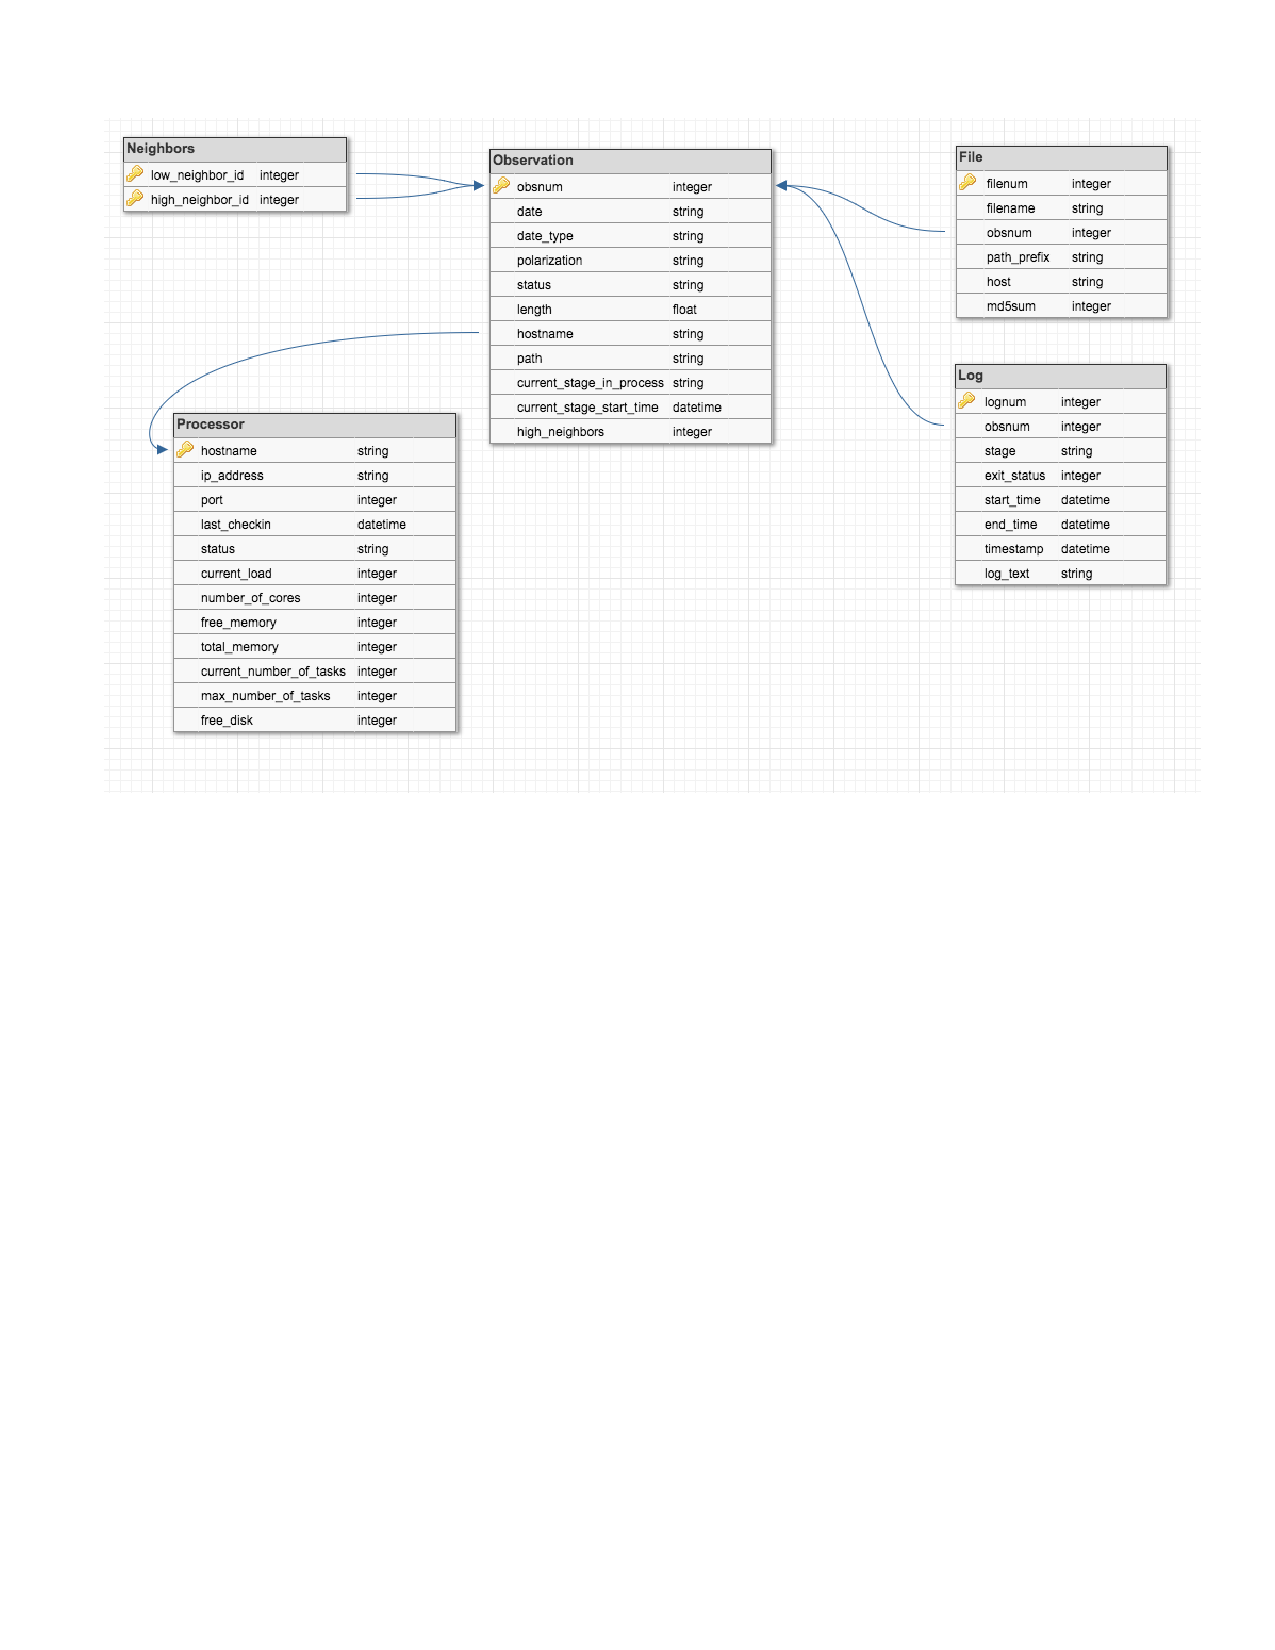
\includegraphics[scale=0.7]{chapters/data_processing/figures/RTP_diagram.pdf}
\caption[The schema of the database used to organize and implement PAPER data compression.]{The schema of the database used to organize and implement PAPER data compression.}
\label{fig:database_schema}
\end{figure}

To implement the compression, per file, the following steps were required:

\begin{enumerate}
\item Copying the file from the storage volume to the cluster. For a single night of data, this required roughly 8 hours.
\item Copying the file from the cluster to the compute node. This required roughly 5 minutes.
\item Generate copy of the file, with metadata corrections. This required roughly 1 minute.
\item Delete the raw file.
\item RFI-flag the high frequency-resolution data. This required roughly 2 minutes.
\item Delete the metadata-corrected file.
\item Acquire time-neighbors to the file in question, and bring them to the RFI-flagged stage. The time required for this stage varied with cluster activity, but usually required roughly 20 minutes.
\item DDR filter the RFI-flagged data, using an high-tolerance iterative CLEAN. This required roughly 20 minutes.
\item RFI flag the compressed data (coarse flagging), saving the flags to a separate file. This required roughly 1 minute.
\item Apply the coarse RFI flags to the \textit{uncompressed}, RFI-flagged data. This required roughly one minute.
\item DDR filter the now twice-RFI-flagged data, using a low-tolerance iterative CLEAN. This required roughly 120 minutes.
\item Copy compressed data to the cluster.
\item Delete the twice-RFI-flagged data.
\item If the once-RFI-flagged data are not required as neighbors, delete them.
\item Delete the compressed data from the compute node.
\item If neighbors have already been compressed, delete them, otherwise begin their compression.
\item After all files are compressed, delete the uncompressed files from the cluster.
\end{enumerate}

In total, this meant that across ten compute nodes, and efficient use of the fact that the neighbors could progress through the processing stages while the central file was being compressed, meant that it took roughly 20 to 24 hours to compress a night of observations. 

\section{Radio Frequency Interference}
\label{sec:RFI}

As noted above, RFI was able to introduce spectral and temporal structure that would cause ringing in the data during compression if it was not flagged. This meant that both identification and characterization of RFI was crucial to the scientific goals of the PAPER and HERA experiments. In Section~\ref{subsec:rfi_paper128}, I present characterization of RFI in the second season of PAPER-128 data. By averaging flags in local time I was able to investigate ``repeat offender'' frequency bands and identify outlying ``quiet'' and ``loud'' days.
In Section~\ref{subsec:rfi_hera19paper19} I analyze RFI flags from the first Internal Data Release (IDR1) of HERA commissioning data, which contained 19 HERA feeds suspended above 5\,m dishes in a close-packed hexagon, and 19 PAPER feeds in the same positions as the central dishes, allowing us to investigate the difference in flagging between feeds at different altitudes.

\subsection{PAPER-128}
\label{subsec:rfi_paper128}

The PAPER-128 2014 observation season ran from 18th June 2014 through the 30th April 2015. During this run, some 150 nights of data were recorded. A ``night'', which I will refer to using the JD at the start of observations, consists of twelve hours of observation from 6pm to 6am South African Standard Time (SAST). Observations as processed by the PAPER correlator are recorded in {\sc miriad} uv files. These files contain visibilities for each antenna pair in the array. Each integration is 20 seconds long over 1024 frequency bins from 100 to 200\,MHz. Each uv file contains 56 integrations per antenna pair, and 72 uv files are recorded per linear polarization (xx, xy, yx, yy) per night.

Early in the PAPER data compression process, visibilities are flagged for RFI. This is accomplished by the {\tt aipy} script \textit{xrfi\_simple.py}, which takes the derivative of the frequency axis of all baselines associated with a single antenna, and flags any frequencies with a derivative $\geqslant 6\sigma$ above the mean. We always flag the band-edges ($\sim$7\,MHz on each side), since these frequencies are not useful to us, and always flag the 137$\pm$0.6\,MHz band associated with ORBCOMM satellite network transmissions. This process is repeated per integration within each uv file and stored in a Python numpy zip (npz) file. This means that any baseline associated with antenna 1 can contribute a flag to the resultant npz file, which in turn is applied to the data.

The result is 280 files of high-time and -frequency resolution files per night per linear polarization containing information about the RFI environment of the HERA site. I report on the properties of these flags in time- and frequency-space over the 2014 observation season. This section is organized it as follows: in Section~\ref{subsubsec:avgprops}, I analyse the average properties of RFI over the season by stacking flags in local time and normalizing appropriately. In Section~\ref{subsubsec:indivprops} I address nights with particularly strange RFI properties. I discuss the implications of my findings in Section~\ref{subsubsec:rfi_paper128_conc}.

\subsubsection{Average Properties}
\label{subsubsec:avgprops}

In order to assess the average properties of the RFI environment, I calculated a weighted average of flags over the season. Over 150 nights, one-time occurrences are washed-out beneath the 1\% level, allowing me to assess persistent issues.

Nominally, each night should grant 3920 integrations-worth of flags over 1024 frequency bins, per linear polarization. In reality, most of the time this holds true, but occasionally not all files are compressible (hence failing to generate flags) or observations fail to start at the correct time (so there are no data to flag). Also, in the event of an X-engine failure within the correlator, contiguous chunks of the band (in eighths, i.e. 25\,MHz across) are flagged-out, usually for the rest of the night.

For this reason, I calculated a weighted average of the flags across the season, but neglected nights with correlator failures or late starts. Weights were simply the number of nights that contained that integration-bin in SAST. The resultant ``flag density waterfall'' is shown in Figure~\ref{fig:rfi_psa128_waterfall}. The color scale is indicative of flagging frequency across the season, and line plots above and to the right of the the waterfall showing the percentage of times and frequencies that were flagged, respectively. 

A summary of the persistent (flagged $\geq1\%$ of the time per channel) RFI frequencies can be found in Table~\ref{tab:rfi_psa128}. I have investigated each frequency and tried to find the most likely source for each. In most cases, this required looking at the properties in time as well as frequency. Others were more obvious from frequency alone, e.g. the 149.8\, MHz transmission frequency from the International Space Station (ISS). Still others I could not track down a convincing explanation for, and these are listed with a `?'. A `?' next to a possible cause indicates that the listed cause is the most prevalent at that frequency, but that the temporal properties of that cause do not necessarily make sense. Many of the characterizations arise from the South African Table of Frequency Allocations (SATFA; \cite{SAFreqTable}).

\begin{figure}[h!]
\centering
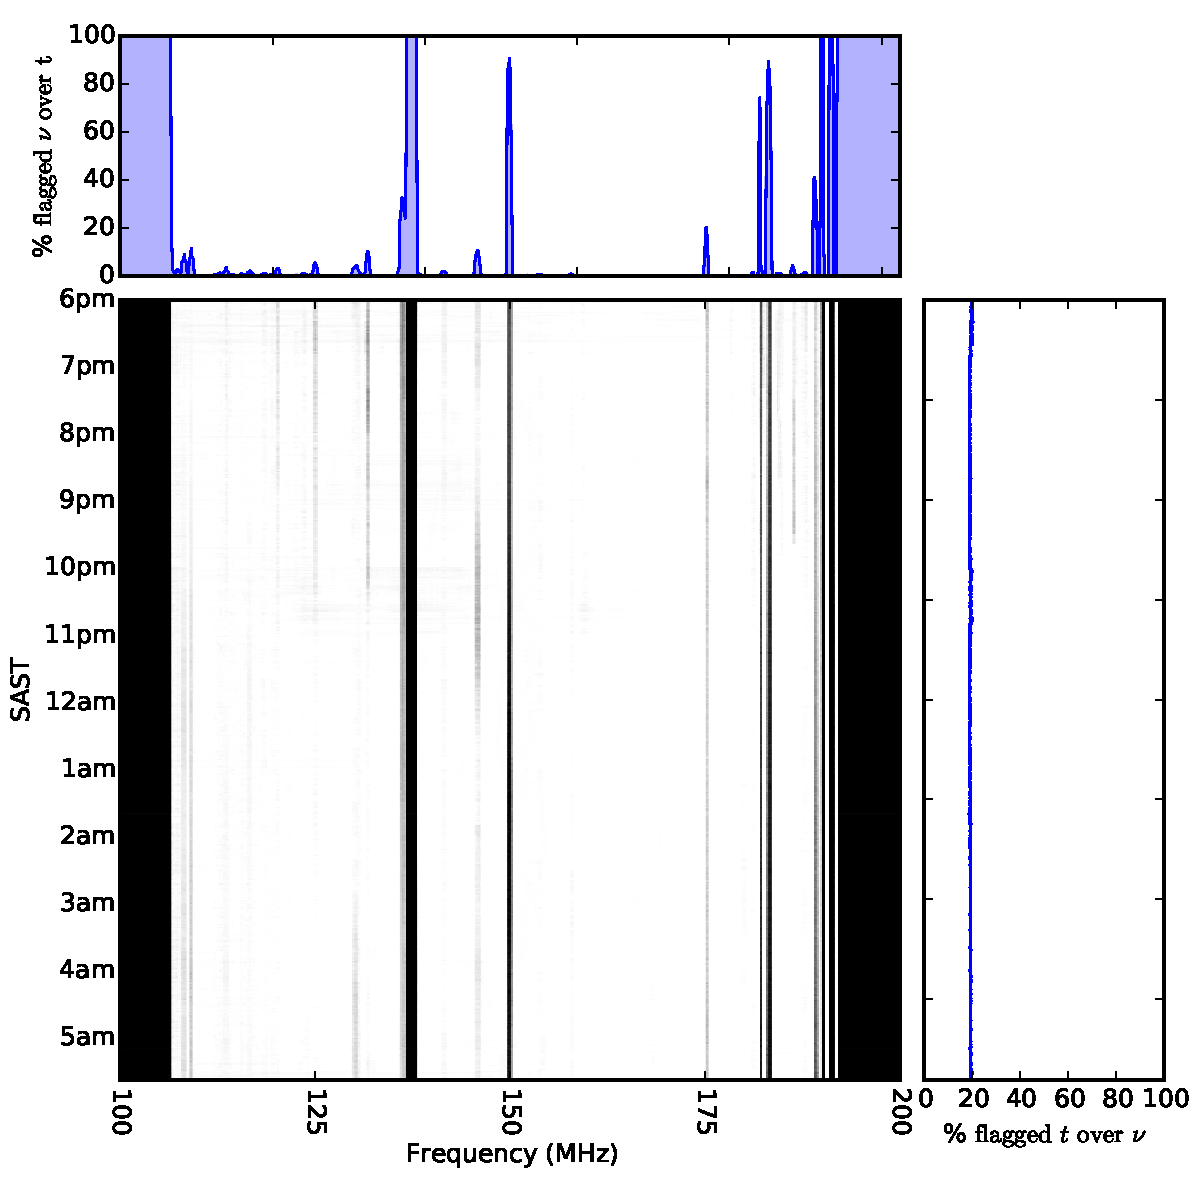
\includegraphics[width=\textwidth]{chapters/data_processing/figures/RFI_all_128.pdf}
\caption[A waterfall plot of RFI flags averaged over 150 days of PAPER-128 data.]{A waterfall plot of RFI flags averaged over 150 days of data. The gridding process is described in the text. Above the waterfall I show the percentage of the season each frequency is flagged, and to the right I show the percentage of frequencies that are flagged per integration.}
\label{fig:rfi_psa128_waterfall}
\end{figure}

\begin{deluxetable}{llll}
\centering
\label{tab:rfi_psa128}
\tablewidth{0pt}
\tablecaption{PAPER-128 RFI frequencies and brief characterization for the averaged flags.}
\tabletypesize{\footnotesize}
\tablehead{
\colhead{$\nu$} & \colhead{Flagged} & \colhead{Cause} & \colhead{Notes or} \\
\colhead{MHz} & \colhead{\%} & \colhead{(Possible)} & \colhead{Time (SAST) Characterization} \\
}
\startdata
103	$\pm$	3	&	100	&	BAND EDGE	&	Built-in to flagger.	\\
107.25	$\pm$	0.25	&	2.6	&	FM radio	&	Constant background at 2\% level	\\
107.55	$\pm$	0.05	&	1.9	&	FM radio	&	Constant background at 2\% level	\\
108.1	$\pm$	0.4	&	9	&	FM radio?	&	Rises with time, peaking at midnight and 4am	\\
109	$\pm$	0.4	&	11.5	&	FM radio?	&	Rises with time, peaking around 4am	\\
112.8	$\pm$	0.1	&	1.4	&	Aircraft?	&	Constant background at 1\% level	\\
114.05	$\pm$	0.85	&	3.7	&	?1	&	Decreases till midnight; peak at 4am	\\
116.55	$\pm$	0.35	&	2.2	&	?2	&	Peak at midnight	\\
120.15	$\pm$	0.35	&	3.2	&	Aircraft	&	Roughly follows CPT$\leftrightarrow$JNB flight times	\\
124.95	$\pm$	0.35	&	5.5	&	Aircraft	&	Roughly follows CPT$\leftrightarrow$JNB flight times	\\
130.25	$\pm$	0.55	&	4.3	&	?3	&	Falls (7pm) and rises (3am) steeply 	\\
131.75	$\pm$	0.35	&	10.3	&	Aircraft?	&	Peaks at 6:30, 7:30, 8:30, 9:30, 10 and then a steep falloff	\\
136.05	$\pm$	0.45	&	33.1	&	Radar?	&	Decreases over night	\\
137.35	$\pm$	0.85	&	100	&	ORBCOMM	&		\\
141.45	$\pm$	0.35	&	2.1	&	Mobile phones?	&	High until 9pm, then at background 1\% level	\\
145.85	$\pm$	0.45	&	10.7	&	Amateur radio& Strong 9pm-1am -- this is the official downlink for ISS-HAM	\\
149.75	$\pm$	0.55	&	90.7	&	ISS	&	``Beeps'', but in stacked data peaks 2am	\\
175.15	$\pm$	0.35	&	20.5	&	VHF TV	 (video) &	 Channel 4. Peaks at 8:30pm, then falls to background 7\%	\\
181.15	$\pm$	0.15	&	1.6	&	VHF TV (audio) & Channel 4. 2\% level turns-off at 10pm	\\
182.15	$\pm$	0.35	&	75	&	?4	&	Decreases until 10pm (to ~15\%), when it begins a slow rise again	\\
183.2	$\pm$	0.5	&	89.7	&	VHF TV (video)	&	Channel 5. Rises throughout night. 	\\
186.25	$\pm$	0.35	&	4.6	&	?5	&	Extreme turn-off at 9:45	\\
189.15	$\pm$	0.35	&	41.4	&	VHF TV (audio)	&	Channel 5. Rises throughout night. 	\\
189.9	$\pm$	0.4	&	100	&	VHF TV 	&	Channel 6. Built-in to flagger. \\
191.1	$\pm$	0.3	&	100	&	VHF TV 	&	Channel 7. Built-in to flagger. \\
196	$\pm$	4	&	100	&	BAND EDGE	&
\enddata
\end{deluxetable}

Figure~\ref{fig:rfi_psa128_freqflags} shows the detail of the top panel of Figure~\ref{fig:rfi_psa128_waterfall}. This figure highlights the broad swath of the band from roughly 150 to 180\,MHz that was, on average, clear of RFI. This roughly corresponds to 21\,cm redshifts $z=6.9$ to 8.5. This is one of the reasons that the \cite{Parsons.14} and \cite{Ali.15} limits on the 21\,cm power spectrum concentrated on this redshift range -- there were simply more unflagged data to average-down with. \cite{Furlanetto.06} show that the $z\sim8$ universe can be considered roughly coeval over an $\sim$8\,MHz bandwidth. As such, the 30\,MHz chunk could be used to create $\sim$3 power spectra, as demonstrated in \cite{Jacobs.15}. As we show below, the deactivation of VHF TV broadcasts could enable measurements up to the band edge.

\begin{figure}[h!]
\centering
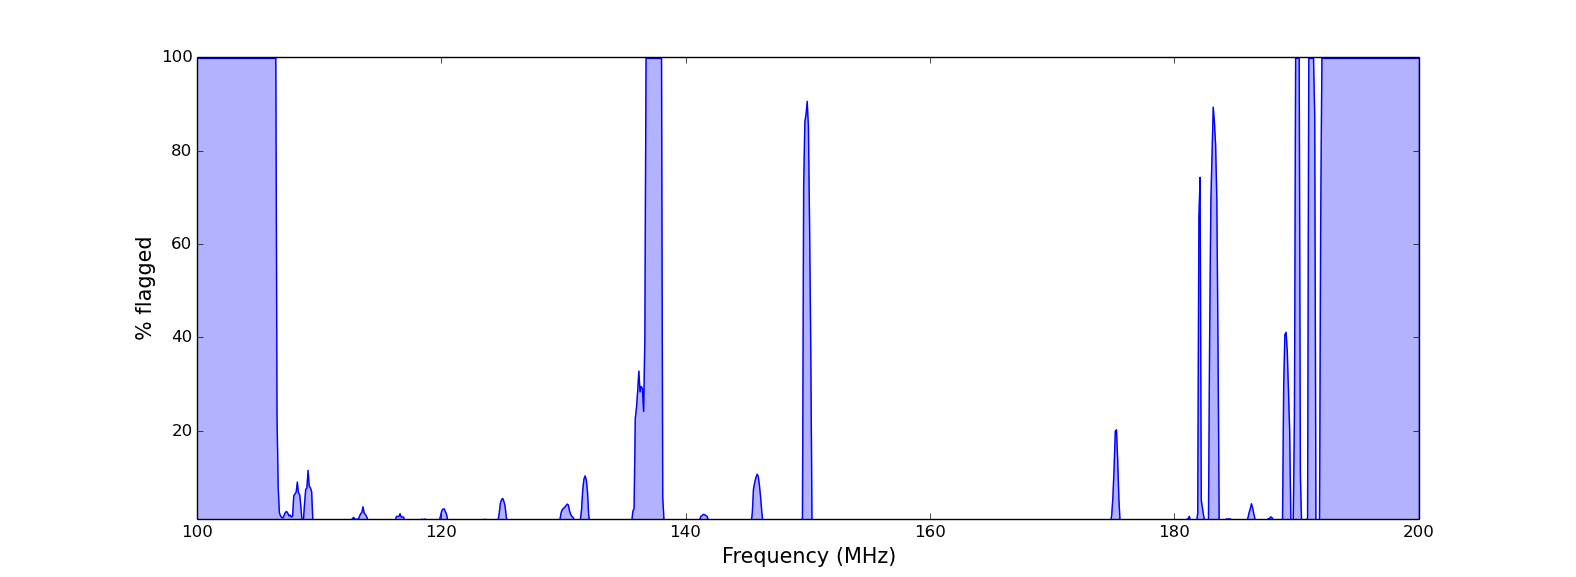
\includegraphics[width=\textwidth]{chapters/data_processing/figures/RFI_149days_freq.png}
\caption{The percentage of time that each frequency was flagged over the season.}
\label{fig:rfi_psa128_freqflags}
\end{figure}

\subsubsection*{FM Radio}

SATFA lists the frequency band 87.5--108\,MHz as available for FM radio broadcasts, leading me to postulate that the low-level RFI we observed in the 107.25	$\pm$	0.25 and 107.55	$\pm$	0.05\,MHz bands had FM radio as the leading cause. The 108.1	$\pm$	0.4 and 109	$\pm$	0.4\,MHz bands were outside of the official range, and exhibit odd temporal properties for human activity -- two peaks at midnight and 4am -- with a increasing number of flags throughout the average night (see Figure~\ref{fig:rfi_psa128_FMradio}). \\

\begin{figure}[h!]
\centering
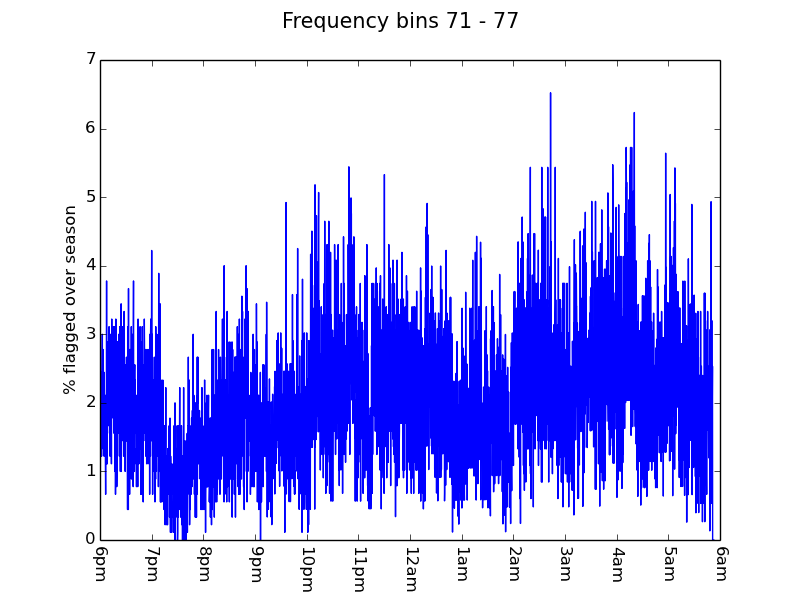
\includegraphics[width=0.4\textwidth]{chapters/data_processing/figures/FB_71_77.png}
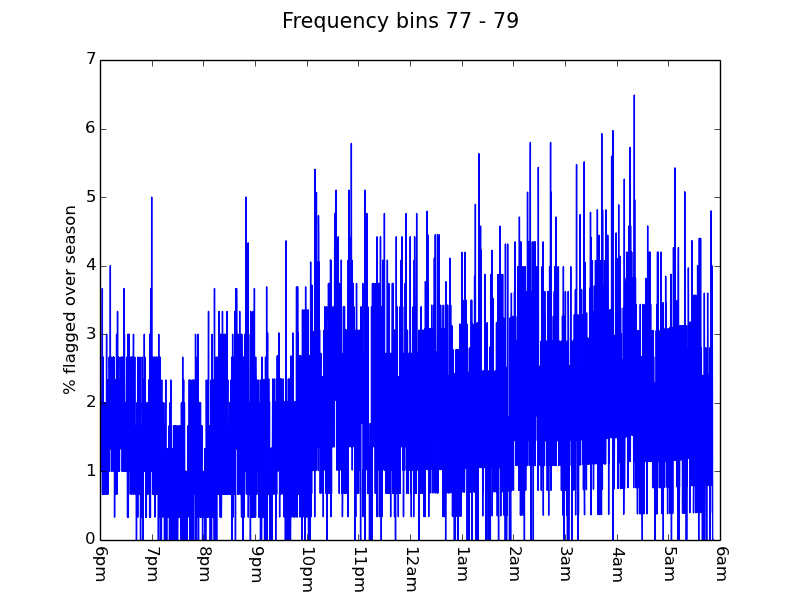
\includegraphics[width=0.4\textwidth]{chapters/data_processing/figures/FB_77_79.png}
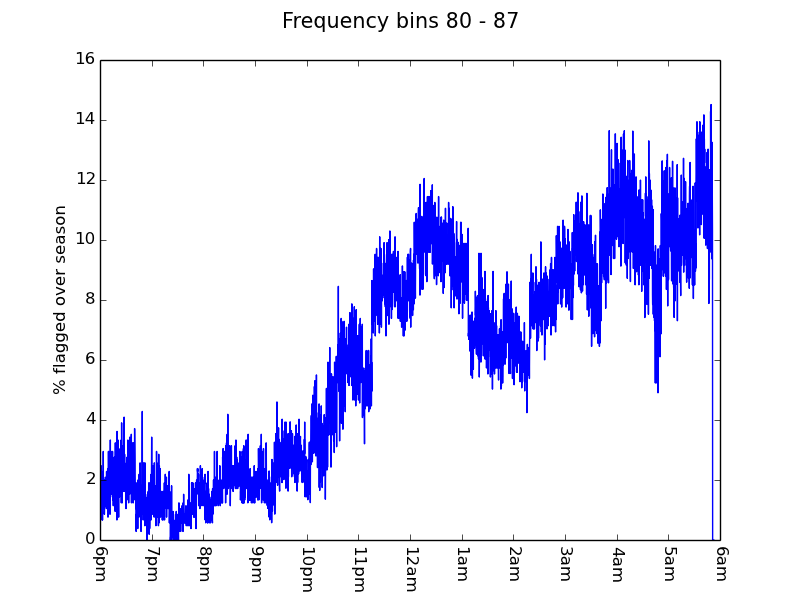
\includegraphics[width=0.4\textwidth]{chapters/data_processing/figures/FB_80_87.png}
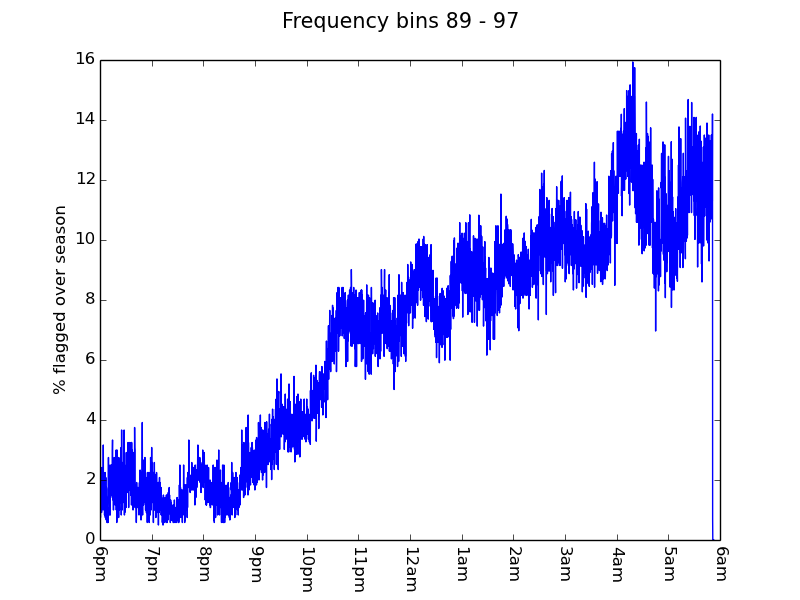
\includegraphics[width=0.4\textwidth]{chapters/data_processing/figures/FB_89_97.png}
\caption[Possible FM radio contamination.]{Possible FM radio contamination in the \textit{Top, left to right}: 107.25$\pm$0.25 and 107.55$\pm$0.05\,MHz bands, and \textit{Bottom, left to right}: 108.1$\pm$0.4 and 109$\pm$0.4\,MHz bands.}
\label{fig:rfi_psa128_FMradio}
\end{figure}

\subsubsection*{Aircraft communications}
It was difficult to argue that the 112.1$\pm$0.1\,MHz signal is caused by aircraft communications since it maintained a constant background level. However, SATFA listed this frequency as reserved for aircraft communications and it has been used in the past as a calibration frequency for aircraft instruments \cite{AircraftCalibrationFreqs}.\\

The other aircraft frequencies were obvious, because they closely traced the 2-hour flight from Cape Town to Johannesburg\footnote{Credit to Danny Jacobs for first spotting this and noting it in an internal PAPER circular in December 2009.}. 
An example (120.15$\pm$0.35\,MHz) is shown in Figure~\ref{fig:rfi_psa128_aircraft}. SATFA reserved frequencies 108--117.975\,MHz for aeronautical radionavigation and 117.975--137\,MHz for aeronautical mobile. In Table~\ref{tab:rfi_psa128} I listed 131.75$\pm$0.35\,MHz as caused by aircraft since it falls in the aeronautical mobile band, but it does not follow the flight patterns as closely as the other bands.\\

\begin{figure}[h!]
\centering
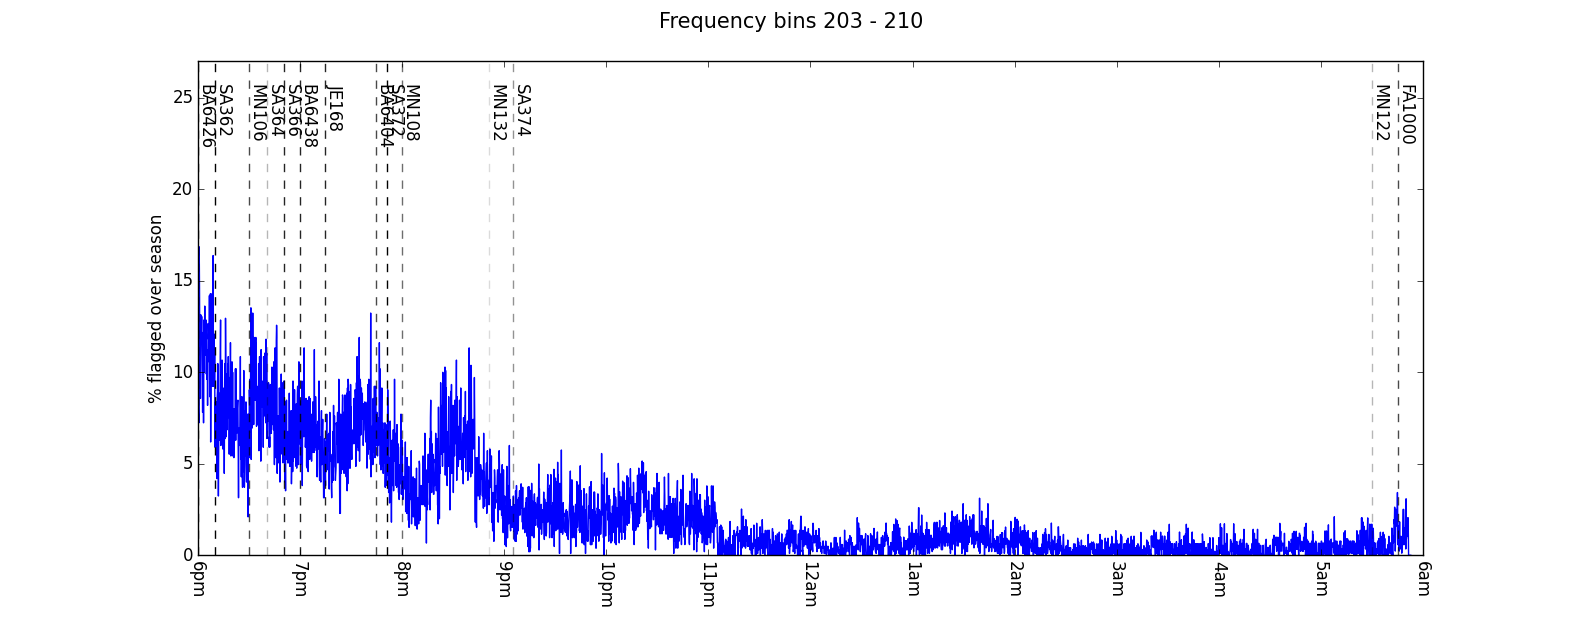
\includegraphics[width=\textwidth]{/Users/saulkohn/Documents/thesis/chapters/data_processing/figures/airlines.png}
\caption[Flights from Cape Town to Johannesburg correspond to RFI in the 120.15$\pm$0.35\,MHz channels.]{
Flights from Cape Town to Johannesburg correspond to RFI in the 120.15$\pm$0.35\,MHz channels. Vertical dashed lines indicate a flight leaving Cape Town (flights from Johannesburg are roughly concurrent) and the flight code is listed. The transparency of a line is inversely proportional to how many days a week that flight is scheduled for. The flight is 2 to 2.5 hours long -- and about 2 hours after the last flight of the day, the flags fall to background level (but notably, not always to zero).}
\label{fig:rfi_psa128_aircraft}
\end{figure} 

\subsubsection*{Orbital communications}
ORBCOMM Inc.'s constellation of 29 LEO communication satellites is a well-known contaminant of the low-frequency sky, dominating over any astronomical signal at 137--138\,MHz (although each satellite emits within a 20\,kHz band). For this reason there was built-in flagging at 137.35$\pm$0.85\,MHz within the compression pipeline.

The largest contaminant without built-in flags in the pipeline were communications from the ISS. The 149.75$\pm$0.55\,MHz transmissions were semi-regular in time; they `beep'. 

Onboard the ISS are HAM radio devices. Some countries have also launched satellites with these onboard, one of the purposes of which is to provide HAM radio operators something in space to communicate with. These devices are licensed to operate at 145.2 and 145.8\,MHz, and SATFA listed the 144-146\,MHz band as reserved for `Amateur--Satellite' communications. We detected RFI at 145.85$\pm$0.45\,MHz, although strong signal across $\sim$10\% of the season that occurs 9pm-1am argues against human operation.

\subsubsection*{Mobile phones and VHF TV}
A weak RFI signal at 141.45$\pm$0.35\,MHz was within the `mobile 1 BTX'  and aeronautical mobile band in SATFA, but other than this single listing I did not build a strong case for the signal's cause.

VHF TV is broadcast over specifically-spaced video and audio frequencies. The strong signals at 183.2$\pm$0.5\,MHz and 189.15$\pm$0.35\,MHz had almost identical gradients for the percentage of flagging as a function of time of night. These frequencies corresponded exactly to Channel 5 of South African System I 625-line VHF TV signals for video and audio transmission, respectively. Similarly, the weaker signals at 175.15$\pm$0.35	 and 181.15$\pm$0.15\,MHz corresponded to Channel 4's video and audio transmission, respectively, but they did not share the same temporal properties.

\subsubsection*{Unidentified sources}

There were 5 RFI frequencies in the averaged data that I could not identify the sources of:  weak emissions (flagged $<5\%$ of the season) at 114.05$\pm$0.85, 116.55$\pm$0.35, 130.25$\pm$0.55 and 186.25$\pm$0.35\,MHz, and one strong emission at 182.15$\pm$0.35\,MHz. The variation of each source with time is shown in Figure~\ref{fig:rfi_psa128_unidentified}. The 186.25$\pm$0.35\,MHz had a sharp turn-off around 9:45pm each night, suggesting that it originated from some kind of automated device.\\

\begin{figure}[h!]
\centering
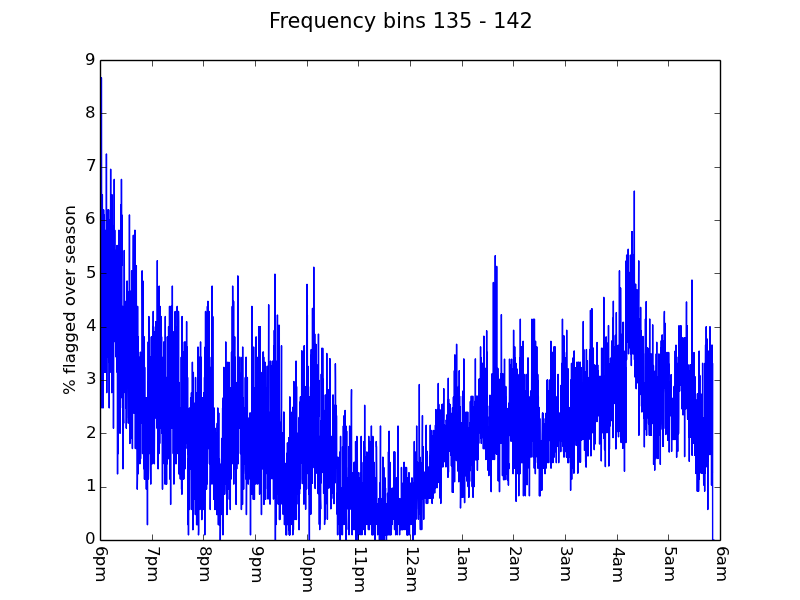
\includegraphics[width=0.4\textwidth]{chapters/data_processing/figures/FB_135_142.png}
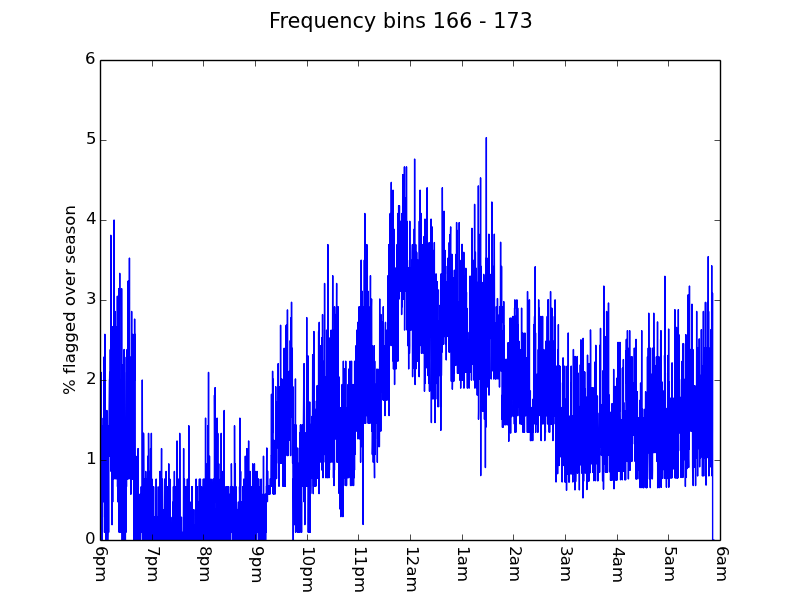
\includegraphics[width=0.4\textwidth]{chapters/data_processing/figures/FB_166_173.png}
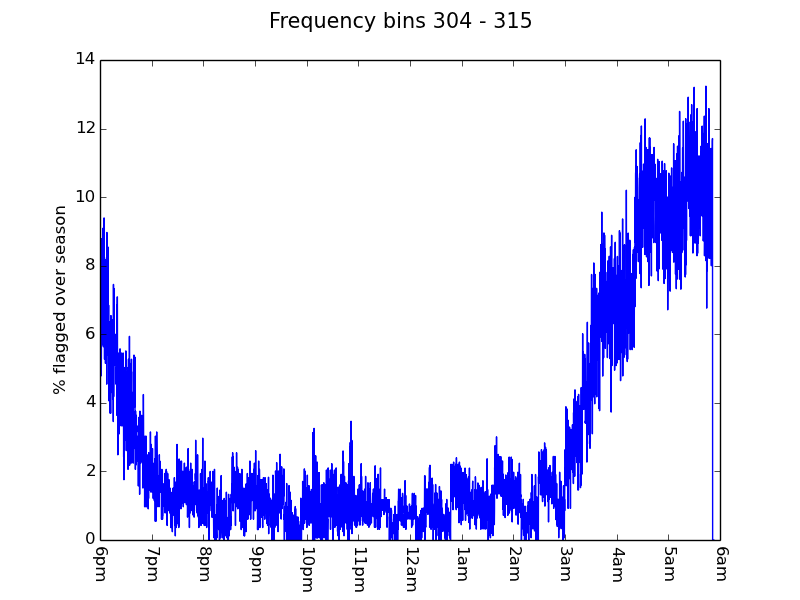
\includegraphics[width=0.4\textwidth]{chapters/data_processing/figures/FB_304_315.png}
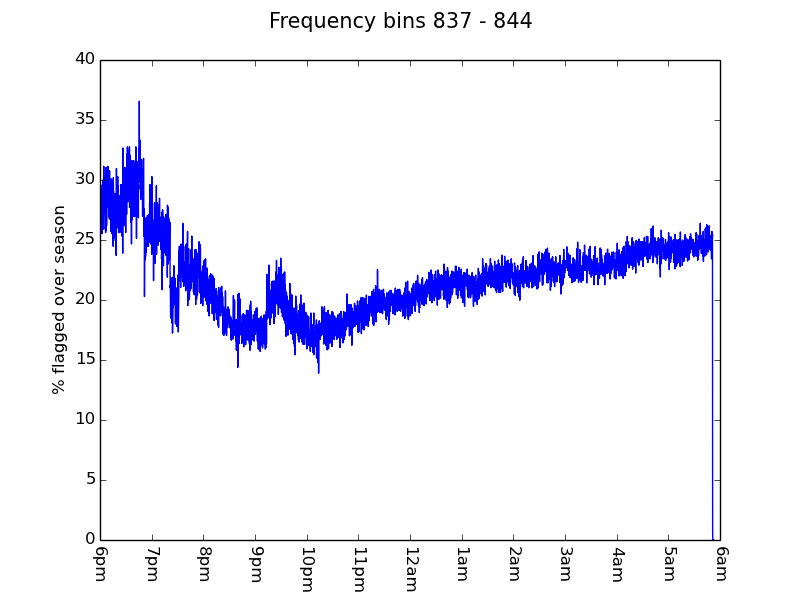
\includegraphics[width=0.4\textwidth]{chapters/data_processing/figures/FB_837_844.png}
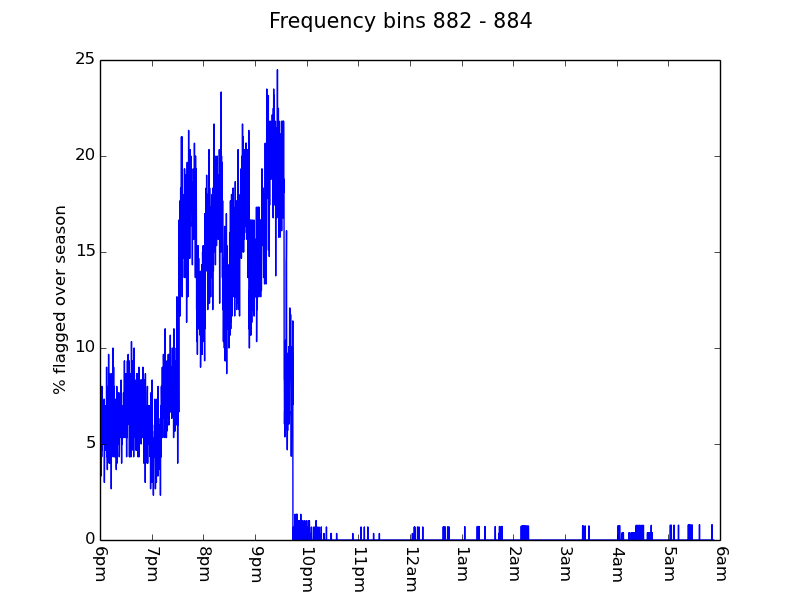
\includegraphics[width=0.4\textwidth]{chapters/data_processing/figures/FB_882_884.png}
\caption[The temporal profile of the 5 RFI frequencies with unidentified causes.]{The temporal profile of the 5 RFI frequencies with unidentified causes. \textit{Top, left to right:} 114.05$\pm$0.85 and 116.55$\pm$0.35\,MHz. \textit{Middle, left to right:} 130.25$\pm$0.55 and 182.15$\pm$0.35\,MHz. \textit{Bottom:} 186.25$\pm$0.35\,MHz. The 182.15$\pm$0.35\,MHz frequency is flagged a large amount of the time, making it our most-offending unidentified source.}
\label{fig:rfi_psa128_unidentified}
\end{figure}

\subsubsection{Individual Properties}
\label{subsubsec:indivprops}

Using the flags per night, I was able to assess the total number of flags as a percentage of the waterfall (i.e. $N_{\rm flags}/(3920\times1024)$). The average flagging per night was 19.2$\pm$0.5\%, which was dominated by the permanent flagging of ORBCOMM and band edges. Four nights deviated from the average by a $\geq 2\sigma$ excess: JDs 2456965, 2456732, 2456958 and 2457038. Their flag waterfalls are shown in Figure~\ref{fig:rfi_psa128_worst} (2456732, 2456958 and 2457038) and Figure~\ref{fig:rfi_psa128_wandering} (2456965). While the strange nature of night 2456965 is discussed below, the three others followed the pattern of having strong contamination from FM and aircraft communication bands, but also had broadband `pulses' up to about 20 minutes in length. The source of these broadband pulses is not well understood, although it was clear that ORBCOMM tends to spill outside of its allocated band on occasion.

\begin{figure}[h!]
\centering
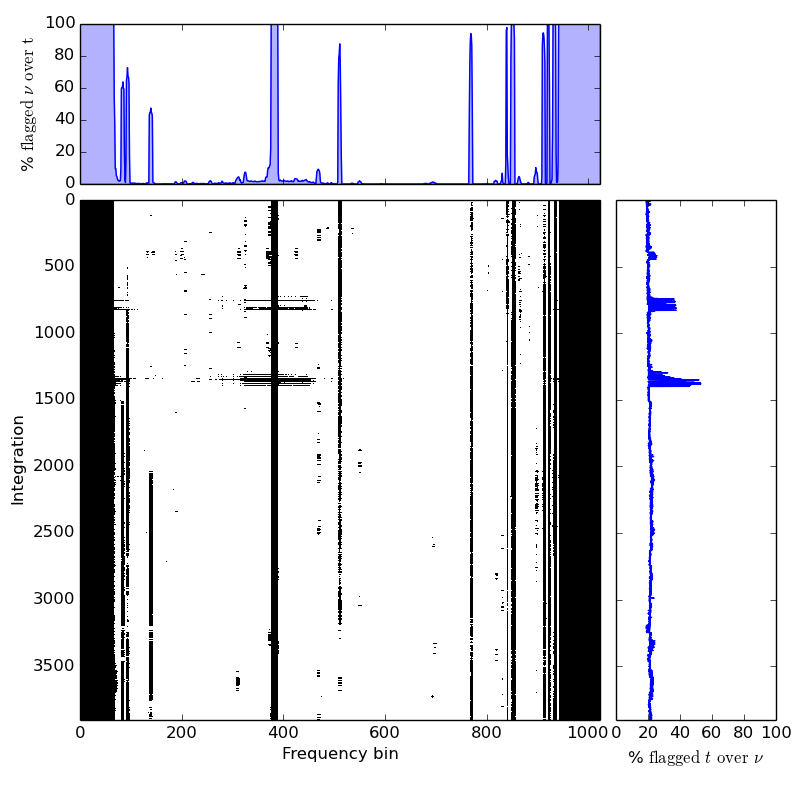
\includegraphics[width=0.3\textwidth]{chapters/data_processing/figures/2456732RFI.png}
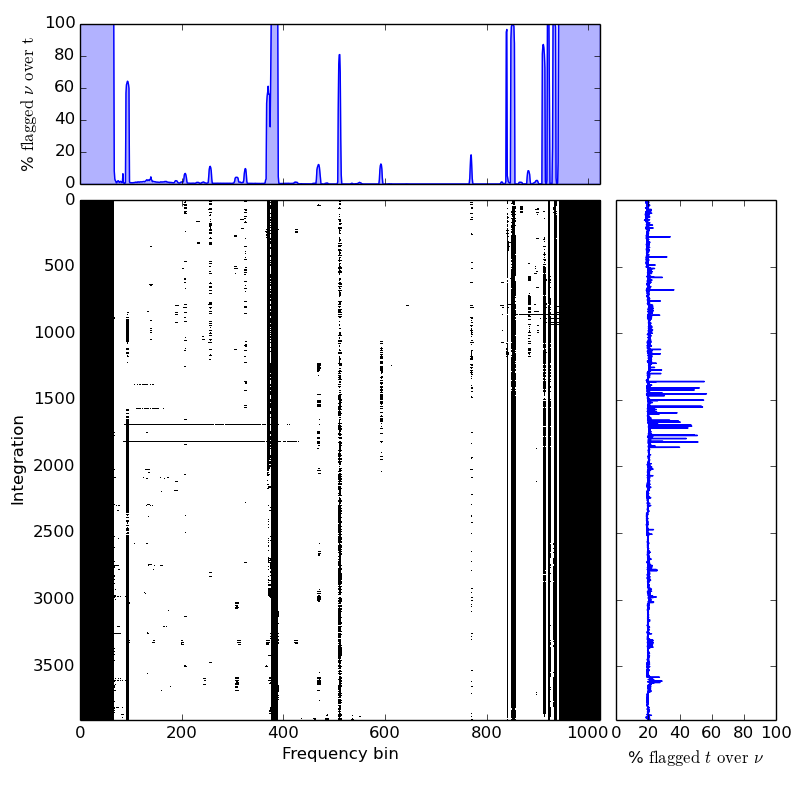
\includegraphics[width=0.3\textwidth]{chapters/data_processing/figures/2456958RFI.png}
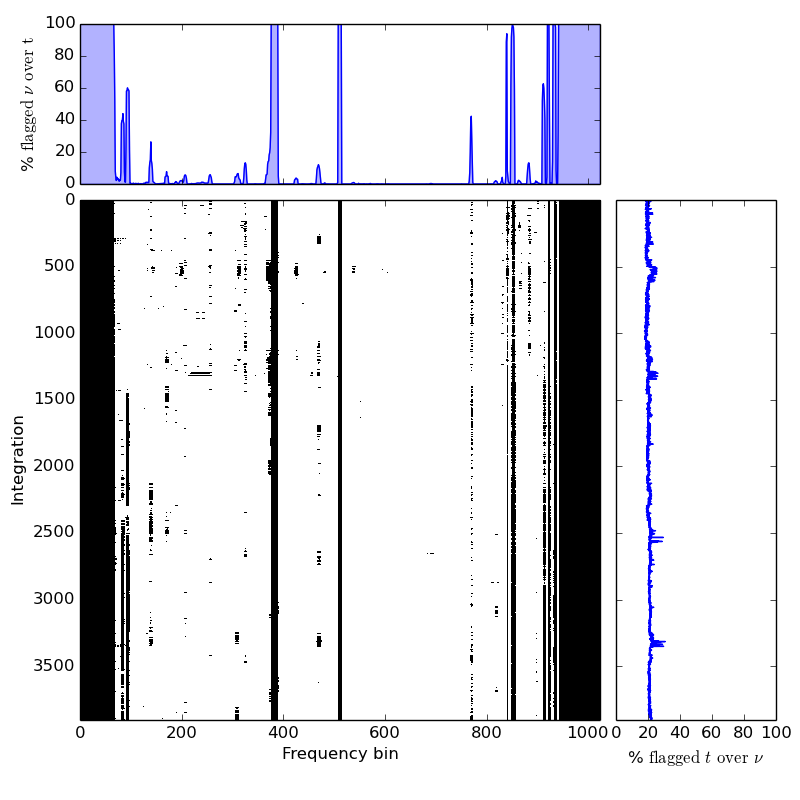
\includegraphics[width=0.3\textwidth]{chapters/data_processing/figures/2457038RFI.png}
\caption[Waterfalls of RFI flags for nights 2456732, 2456958 and 2457038.]{\textit{Left to right:} waterfalls of flags for nights 2456732, 2456958 and 2457038. These three nights, along with 2456965, are $>$20.2\% flagged; $>2\sigma$ above the average flagging amount per night.}
\label{fig:rfi_psa128_worst}
\end{figure}


JD 2456965 was easily the worst offender, and it exhibited a strange signal that wanders in frequency and time close to the ISS band. An event of note on this date (23rd November 2014) was a Soyuz FG launch that docked with the ISS -- this may have been a signature of their transmissions\footnote{The internet also suggests... less plausible explanations: \url{https://www.youtube.com/watch?t=11&v=VtZx8iPO4zs}. }.
Similar signals were seen on 2456898 (28th August 2014; although only at the beginning of the night) and 2456924 (23rd September 2014). There was no listed orbital or suborbital activity for 2456898. There was an US ICBM test off of the coast of Virginia on 2456924, but this was probably not the cause of the RFI. The flag waterfalls for these nights are shown in Figure~\ref{fig:rfi_psa128_wandering}.\\

\begin{figure}[h!]
\centering
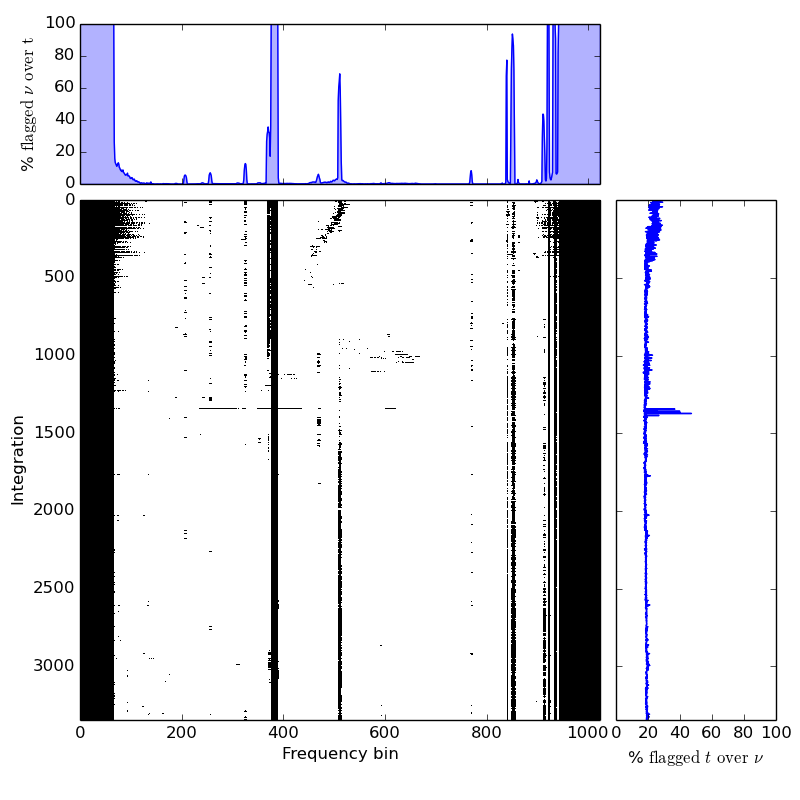
\includegraphics[width=0.3\textwidth]{chapters/data_processing/figures/2456898RFI.png}
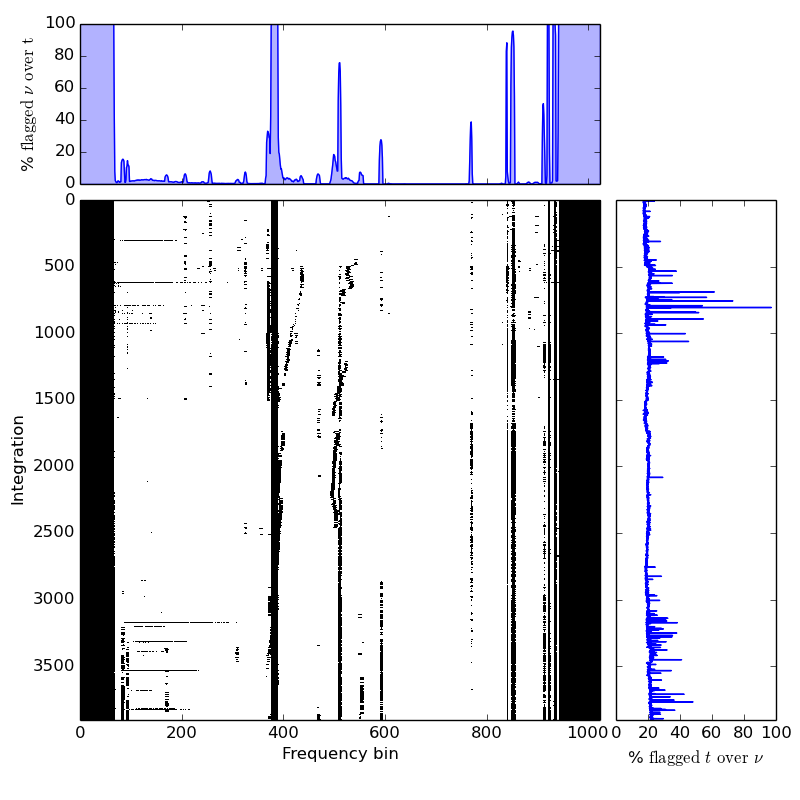
\includegraphics[width=0.3\textwidth]{chapters/data_processing/figures/2456924RFI.png}
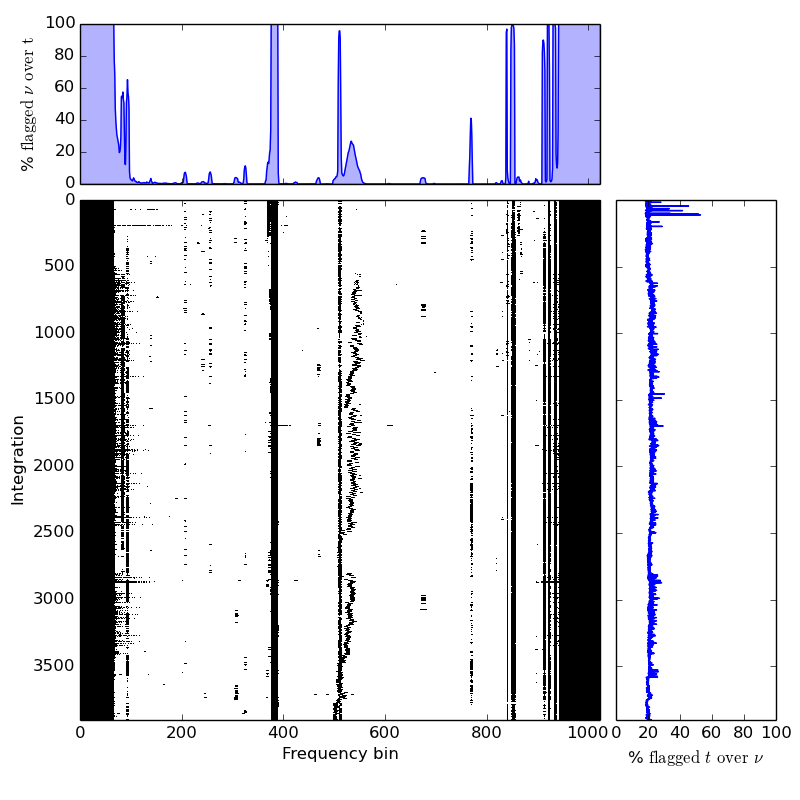
\includegraphics[width=0.3\textwidth]{chapters/data_processing/figures/2456965RFI.png}
\caption[Waterfalls of RFI flags for nights 2456898, 2456924 and 2456965]{\textit{Left to right:} waterfalls of flags for nights 2456898, 2456924 and 2456965. These three nights exhibit a strange behaviour of RFI that changes in frequency and time. JD 2456965 is by far the worst, and during this night as well as 2456898, we see a broadband `comb' of flagged frequencies near the band edges}
\label{fig:rfi_psa128_wandering}
\end{figure}

Another property that the flag waterfalls in Figures~\ref{fig:rfi_psa128_worst} and \ref{fig:rfi_psa128_wandering} highlight is the presence of broadband RFI signals, typically present at frequencies lower than the ORBCOMM band. However, while we flagged at the low-end of the band (which had higher noise levels to begin with), it is likely that such broadband pulses dominated the band at those times, and that we failed to flag all of the integrations. Our flagging routine \textit{xrfi\_simple.py} does contain a thresholding option for flagging the entire integration given some arbitrary number of frequencies flagged during that integration: some experimentation will be required to decide if that threshold should change.

\subsubsection{Discussion}
\label{subsubsec:rfi_paper128_conc}

Based on my findings, I was able to recommend some actions that could be taken in the KRQZ to enable better measurements:
\begin{itemize}
\item  Steps to reduce and ideally eliminate the VHF TV transmissions in the area would be very helpful, since these were clearly interfering with our measurements in the high-end of the band.
\item The ISS 149.75$\pm$0.55\,MHz band should be permanently flagged within the compression pipeline.
\item Pursuing re-routing of flight paths will not do much to help: we see aircraft signals for the duration of their flight, not just when they're over the Karoo.
\item A lower threshold for identifying broadband RFI should be investigated.
\end{itemize}

A new, lower-frequency feed is currently under development by the HERA analog group. This would nominally allow measurements to be taken in the range 50--250\,MHz, allowing science observations of the Dark Ages and the post-reionization Universe. It should be noted that at the lowest frequencies FM radio will be a constant harassment to these measurements. At the higher frequencies, VHF TV will be the primary contaminant, but should be much easier to remove as it is both narrow-band and within the KRQZ's power to shut off.

\subsection{HERA-19 and PAPER-19}
\label{subsec:rfi_hera19paper19}

The HERA-19 IDR1 consisted of four subarrays: the HERA-19 hexagon of dishes (the `HERA Hex'), a hexagon of 19 PAPER dipoles in the exact positions of not-yet-constructed HERA dishes (the `PAPER Hex'), an imaging array and an experimental array for polarization measurements. I will concentrate on the two Hexes in this Section. I analyzed RFI as flagged in the linear \textit{xx}-polarization only. Asymmetric beams can in principle receive different RFI events for different linear polarizations, but analysis of that was outside the scope of this diagnostic study.

IDR1 consisted of one `golden day', JD 2457458. This ran from 6pm on March 10th 2016 to 6am the following day. This gave, per baseline, roughly 4000 integrations of 10 seconds each over 1024, 100~kHz frequency channels from 100 to 200~MHz.

In order to flag RFI I used the {\tt aipy} script \textit{xrfi\_simple.py}. I took the union of all baseline flags as data to analyze. Unlike in Section~\ref{subsec:rfi_paper128}, these data did not have a-priori flagging of band edges, which allowed me to make a more complete study of RFI in the HERA band. I did have to implement custom flags in order to get more than a zeroth-order view of the RFI (since these would dominate the flagging routine unless they are flagged already), but my results from Section~\ref{subsec:rfi_paper128}  gave a better idea of what was flagged to get there. 

Below I present measurements of high-power, mostly narrow-band RFI channels as flagged in HERA Hex data and PAPER Hex data separately. In both cases, I was able to list any channels that are flagged for $\geqslant 1\%$ of the night. I could then compare the flagging Hex-to-Hex, and to PAPER-128.

\subsubsection{HERA Hex RFI}
\label{subsubsec:rfi_herahex}

Table~\ref{tab:rfi_herahex} shows all narrowband frequency ranges flagged in HERA-19 visibilities, with columns of the frequency range in MHz, \% flagging over time, plausible identification, whether or not it was identified in PAPER-128 data, and other notes (often details of the possible identification). Frequencies with 100\% flagging indicate manual flags required for {\tt xrfi\_simple} to work on the rest of the channels. 

Clearly, the low-end of the band was swamped by FM radio broadcasts. One notable frequency was the 109.2$\pm$0.3~MHz band, which was heavily flagged in HERA visibilities, but was only flagged a few percent in PAPER-128 data.

As seen before, ORBCOMM satellite emissions spilled out of their allocated 137-138~MHz band down to 136.3~MHz.

There were many narrowband RFI channels, across the band, that PAPER-128 did not pick-up. Most of these were flagged only at low levels, with two exceptions: 111.3$\pm$0.2~MHz and 113.5$\pm$0.1~MHz. Both of these were in the aircraft navigation band. There is some evidence \citep{airforce} that 111.3~MHz band is fir air force communications. The 113.5~MHz band is a known band for radionavigation beacons \citep[`VOR navaids'][]{navaid}.

A particularly annoying `new' emitter was in the 153.8$\pm$0.2~MHz region, which is close to the center of our nominal EoR band. It could correspond to mobile phones being used close to site.

\begin{deluxetable}{lllll}				
\centering														
\label{tab:rfi_herahex}
\tablewidth{0pt}
\tablecaption{RFI as flagged by HERA}
\tabletypesize{\footnotesize}
\tablehead{
\colhead{$\nu$} & \colhead{Flagged} & \colhead{Cause} & \colhead{Seen by} & \colhead{Notes} \\
\colhead{MHz} & \colhead{\%} & \colhead{(Possible)} & \colhead{PAPER-128} &\colhead{} \\
}
\startdata													
100.7	$\pm$	0.2	&	50	&	FM Radio	&	n/a	&	RSG ``Dis Die Een'' Prieska		\\
101.5	$\pm$	0.3	&	36	&	FM Radio	&	n/a	&	RSG ``Dis Die Een'' Calvinia	\\
102.4	$\pm$	0.1	&	100	&	FM Radio	&	n/a	&	RSG ``Dis Die Een'' Carnarvon	\\
102.8	$\pm$	0.3	&	57	&	FM Radio	&	n/a	&	RSG ``Dis Die Een'' Pofadder	\\
104.2	$\pm$	0.1	&	100	&	FM Radio	&	n/a	&	SAfm Prieska	\\
105.1	$\pm$	0.2	&	100	&	FM Radio	&	n/a	&	SAfm Calvinia	\\
106.2	$\pm$	0.3	&	100	&	FM Radio	&	n/a	&	SAfm Carnarvon	\\
106.9	$\pm$	0.1	&	15	&	FM Radio	&	n/a	&	Sentech	\\
107.2	$\pm$	0.1	&	18	&	FM Radio	&	Yes	&		\\
107.8	$\pm$	0.2	&	15	&	FM Radio	&	Yes	&		\\													
108.3	$\pm$	0.1	&	31	&	FM Radio?	&	Yes	&			\\
109.2	$\pm$	0.3	&	93	&	FM Radio?	&	Yes...&	...but not to this degree	\\
111.3	$\pm$	0.2	&	25	&	Air force?	&	No	&		\\
112.5	$\pm$	0.1	&	5	    &	Aircraft?	&	No	&	\\
113.5	$\pm$	0.1	&	21	&	Aircraft    &	No	&	VOR navaids		\\
115.5	$\pm$	0.1	&	3	    &	Navaids?	    &	No	&	\\
115.9	$\pm$	0.1	&	3	    &	Navaids?	    &	No	&	\\
116.6	$\pm$	0.2	&	9	   &	Aircraft?	    &	Yes	&	VOR-DME navaids		\\
120.1	$\pm$	0.2	&	5	&	Aircraft	&	Yes	&	CPT$<->$JNB		\\
125.0$\pm$	0.2	&	6	&	Aircraft	&	Yes	&	CPT$<->$JNB		\\
130.0	$\pm$	0.2	&	4	&	Aircraft	&	No	&	Communication		\\
131.6	$\pm$	0.2	&	15	&	Aircraft	&	Yes	&	KLM OPS		\\
136.4	$\pm$	0.1	&	9	&	ORBCOMM	&	Yes	&					\\
136.7	$\pm$	0.1	&	10	&	ORBCOMM	&	Yes	&					\\
137.4	$\pm$	0.4	&	100	&	ORBCOMM	&	Yes	&				\\
145.7	$\pm$	0.4	&	18	&	ISS/Amateur Radio band	&	Yes	&			\\
149.9	$\pm$	0.1	&	100	&	ISS	&	Yes	&			\\
153.8	$\pm$	0.2	&	7	&	Mobile phones?	&	No	&			\\
175.0	$\pm$	0.1	&	100	&	VHF TV	&	Yes	&	Channel 4 Video		\\
178.3	$\pm$	0.2	&	8	&	VHF TV	&	No	&	Channel 7?		\\
181.2	$\pm$	0.1	&	100	&	VHF TV	&	Yes	&	Channel 4 Audio		\\
182.2  $\pm$	0.2	&	9	&		&	Yes	&			\\
183.5	$\pm$	0.6	&	100	&	VHF TV	&	Yes	&	Channel 5 Video		\\
184.1	$\pm$	0.1	&	2	&	VHF TV?	&	Yes	&	Channel 5?	\\
184.7	$\pm$	0.1	&	6	&	Broadcasting	&	No	&		\\
187.8	$\pm$	0.1	&	4	&		&	No	&		\\
189.1	$\pm$	0.1	&	52	&	VHF TV	&	Yes	&	Channel 5 Audio	\\
190.1	$\pm$	0.3	&	13	&		&	n/a	&		\\
191.1	$\pm$	0.1	&	100	&	VHF TV	&	n/a	&	Channel 7		\\
197.2	$\pm$	0.2	&	18	&		&	n/a	&		\\
199.4	$\pm$	0.5	&	100	&	BAND EDGE	&	n/a	&		\\
\enddata
\end{deluxetable}

\subsubsection{PAPER Hex RFI}
\label{subsubsec:rfi_paperhex}

Table~\ref{tab:rfi_paperhex} has the same description as Table~\ref{tab:rfi_herahex}, but for the PAPER Hex. There were far fewer RFI frequencies flagged in PAPER visibilities, almost all of which were seen by HERA. The only RFI seen by the PAPER Hex and not the HERA Hex was the 123.5$\pm$0.1~MHz emission, which I could find a plausible identification for.

\begin{deluxetable}{lllll}													
\centering														
\label{tab:rfi_paperhex}
\tablewidth{0pt}
\tablecaption{RFI as flagged by the PAPER Hex}	
\tabletypesize{\footnotesize}
\tablehead{
\colhead{$\nu$} & \colhead{Flagged} & \colhead{Cause} & \colhead{Seen by} & \colhead{Notes} \\
\colhead{MHz} & \colhead{\%} & \colhead{(Possible)} & \colhead{PAPER-128} &\colhead{} \\
}
\startdata	
100.0	$\pm$	0.1	&	100	&	BAND EDGE	&	n/a	&		\\		
100.7	$\pm$	0.1	&	11	&	FM Radio	&	n/a	&	RSG ``Dis Die Een'' Calvinia			\\		
101.6	$\pm$	0.2	&	6	&	FM Radio	&	n/a	&	RSG ``Dis Die Een'' Calvinia			\\		
102.4	$\pm$	0.1	&	100	&	FM Radio	&	n/a	&	RSG ``Dis Die Een'' Carnarvon		\\		
102.7	$\pm$	0.1&	100	&	FM Radio	&	n/a	&	RSG ``Dis Die Een'' Pofadder		\\		
104.2	$\pm$	0.2	&	100	&	FM Radio	&	n/a	&	SAfm Prieska		\\		
105.1	$\pm$	0.2	&	100	&	FM Radio	&	n/a	&	SAfm Calvinia	\\		
106.2	$\pm$	0.3	&	100	&	FM Radio	&	n/a	&	SAfm Carnarvon	\\		
																
108.2	$\pm$	0.1	&	3	&	FM Radio?	&	Yes	&		\\		
109.1	$\pm$	0.1  &	26	&	FM Radio?	&	Yes	&		\\		
113.6	$\pm$	0.1	&	2	&	Airplane Communications	&	No	&	VOR navaid			\\		
																
120.2	$\pm$	0.3	&	3	&	Aircraft	&	Yes	&	CPT$<->$JNB		\\		
123.5	$\pm$	0.1	&	1	&		&	No	&	Not seen by HERA			\\		
125.0	$\pm$	0.2	&	6	&	Aircraft	&	Yes	&	CPT$<->$JNB		\\		
130.0	$\pm$	0.3	&	3	&		&	No	&			\\		
131.7	$\pm$	0.2	&	14	&	Aircraft	&	Yes	&				\\		
136.4	$\pm$	0.2	&	6	&	ORBCOMM	&	Yes	&					\\		
136.7	$\pm$	0.2	&	6	&	ORBCOMM	&	Yes	&				\\		
															
137.4	$\pm$	0.4	&	100	&	ORBCOMM	&	Yes	&				\\		
145.8	$\pm$	0.3	&	14	&	ISS/Amateur Radio band	&	Yes	&			\\		
149.9	$\pm$	0.1	&	100	&	ISS	&	Yes	&			\\		
153.8	$\pm$	0.2	&	3	&	Single frequency mobile phones?	&	No	&				\\		
																
175.1	$\pm$	0.2	&	100	&	VHF TV	&	Yes	&	Channel 4 Video				\\		
178.3	$\pm$	0.2	&	100	&	VHF TV	&	No	&	Channel 7?		\\		
181.2	$\pm$	0.1	&	100	&	VHF TV	&	Yes	&	Channel 4 Audio	\\		
183.2	$\pm$	0.2	&	100	&	VHF TV	&	Yes	&	Channel 5 Video			\\		
189.2	$\pm$	0.1	&	100	&	VHF TV	&	Yes	&	Channel 5 Audio			\\		
191.2	$\pm$	0.1	&	100	&	VHF TV	&	n/a	&	Channel 7			\\		
199.8	$\pm$	0.2	&	100	&	BAND EDGE	&	n/a	&			\\
\enddata
\end{deluxetable}

\subsubsection{Hex-to-Hex Comparisons}
\label{subsubsec:hex2hex_comparison}

As mentioned above, the PAPER Hex saw far fewer narrowband RFI channels than HERA does. This highlighted an interesting trade-off between dipoles and dishes: at first glance, one might have expected PAPER dipoles to be more susceptible to RFI given their broader effective beams. However, HERA dipoles are lifted several meters above the ground, and this change in height may have been the source of the greater susceptibility to RFI. RFI comes from the horizon, which would be more easily received in the far sidelobes of the beam.

\begin{figure}[h!]
\centering
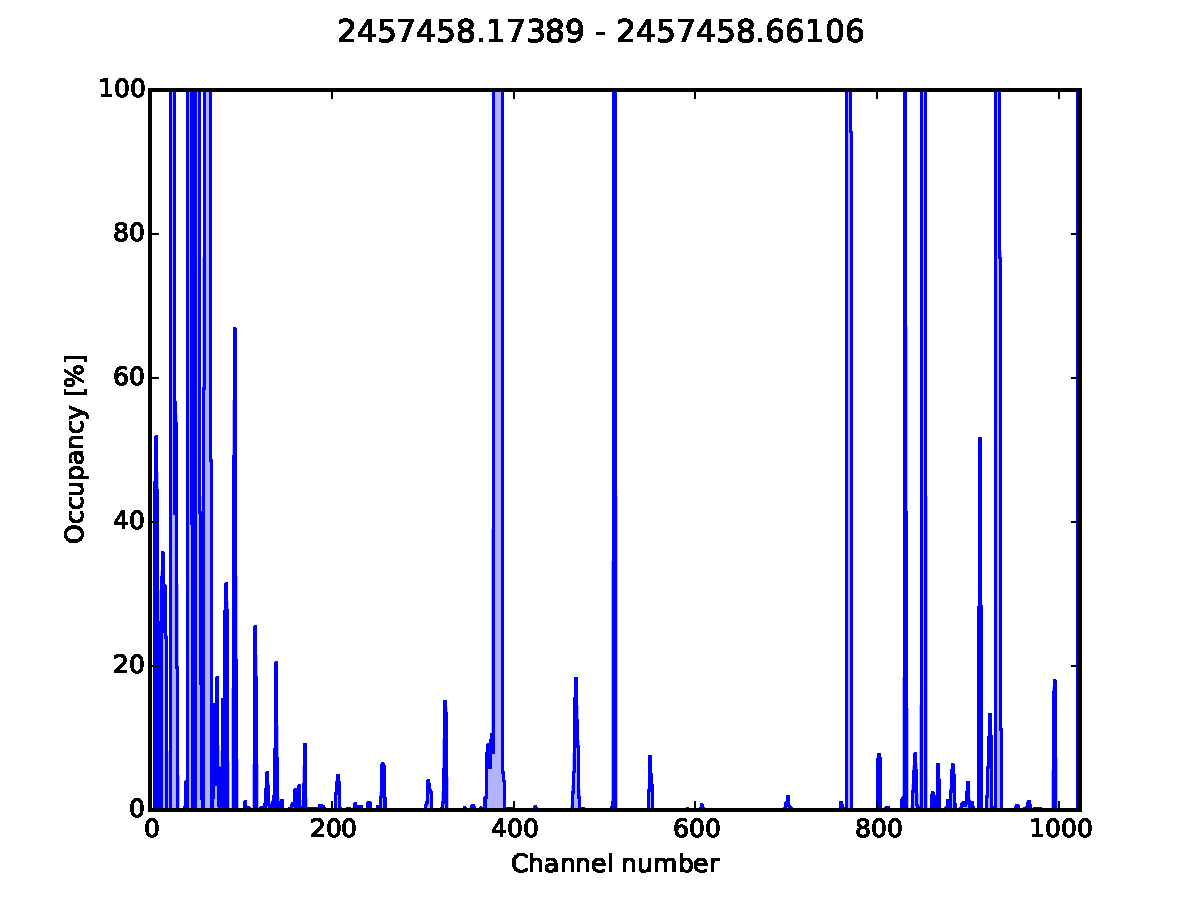
\includegraphics[width=0.45\textwidth]{chapters/data_processing/figures/RFI_HH_spec.pdf}
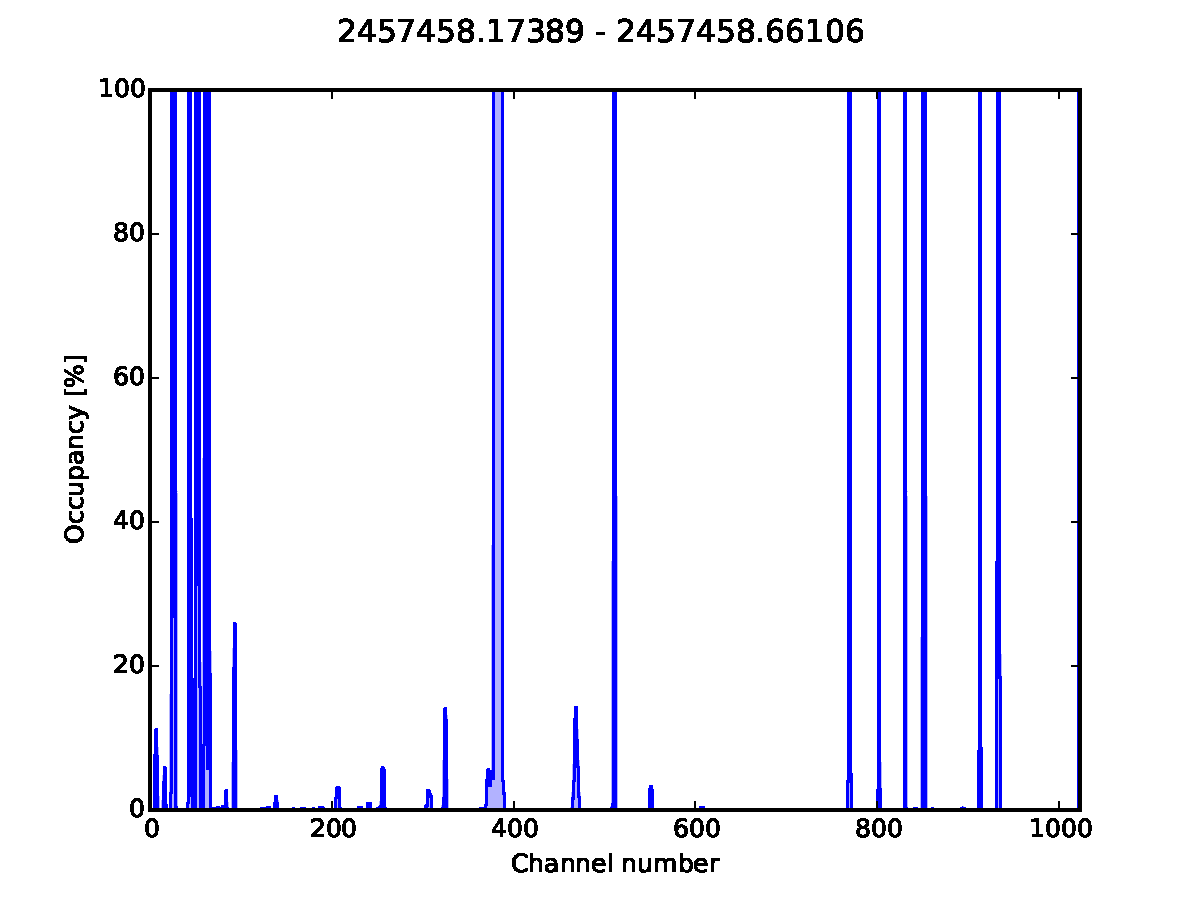
\includegraphics[width=0.45\textwidth]{chapters/data_processing/figures/RFI_PH_spec.pdf}
\caption[Frequency vs. percentage flagging for the HERA Hex and PAPER Hex.]{Frequency vs. percentage flagging for the HERA Hex (\textit{left}) and PAPER Hex (\textit{right}). Any band with greater than 1\% flagging is reported in Tables~\ref{tab:rfi_herahex} and \ref{tab:rfi_paperhex}.}
\label{fig:rfi_spec_hex_comparison}
\end{figure}

Even for the RFI channels they did share, HERA flagged them more often. Taking the difference in percentage-flagging for the common RFI channels (think of the left panel subtracted from the right panel for common channels in Figure~\ref{fig:rfi_spec_hex_comparison}), those channels had an average of 8\% more flagging in HERA visibilities. The difference was particularly high in the aeronautical radionavigation bands, where HERA had on average 38\% more flagging than the PAPER Hex.

Figure~\ref{fig:rfi_hex_waterfalls} shows the flags on a per-sample basis (these were averaged over time to create Figure~\ref{fig:rfi_spec_hex_comparison}). Most apparent was the occupancy of the HERA plot compared to the PAPER Hex one. An important component of this plot is the averages over frequency in the right-hand panels. We saw that the average flagging for a given time sample was about 5\% higher for HERA than for the PAPER Hex, mostly due to the higher occupancy of the FM band. But we also saw something new; HERA appeared to be much more sensitive to broadband bursts of RFI. The PAPER Hex caught one of these events (around 1.30am SAST) at high significance, but most of them hardly rose above average flagging. HERA saw five to seven bursts across the night. 

\begin{figure}
\centering
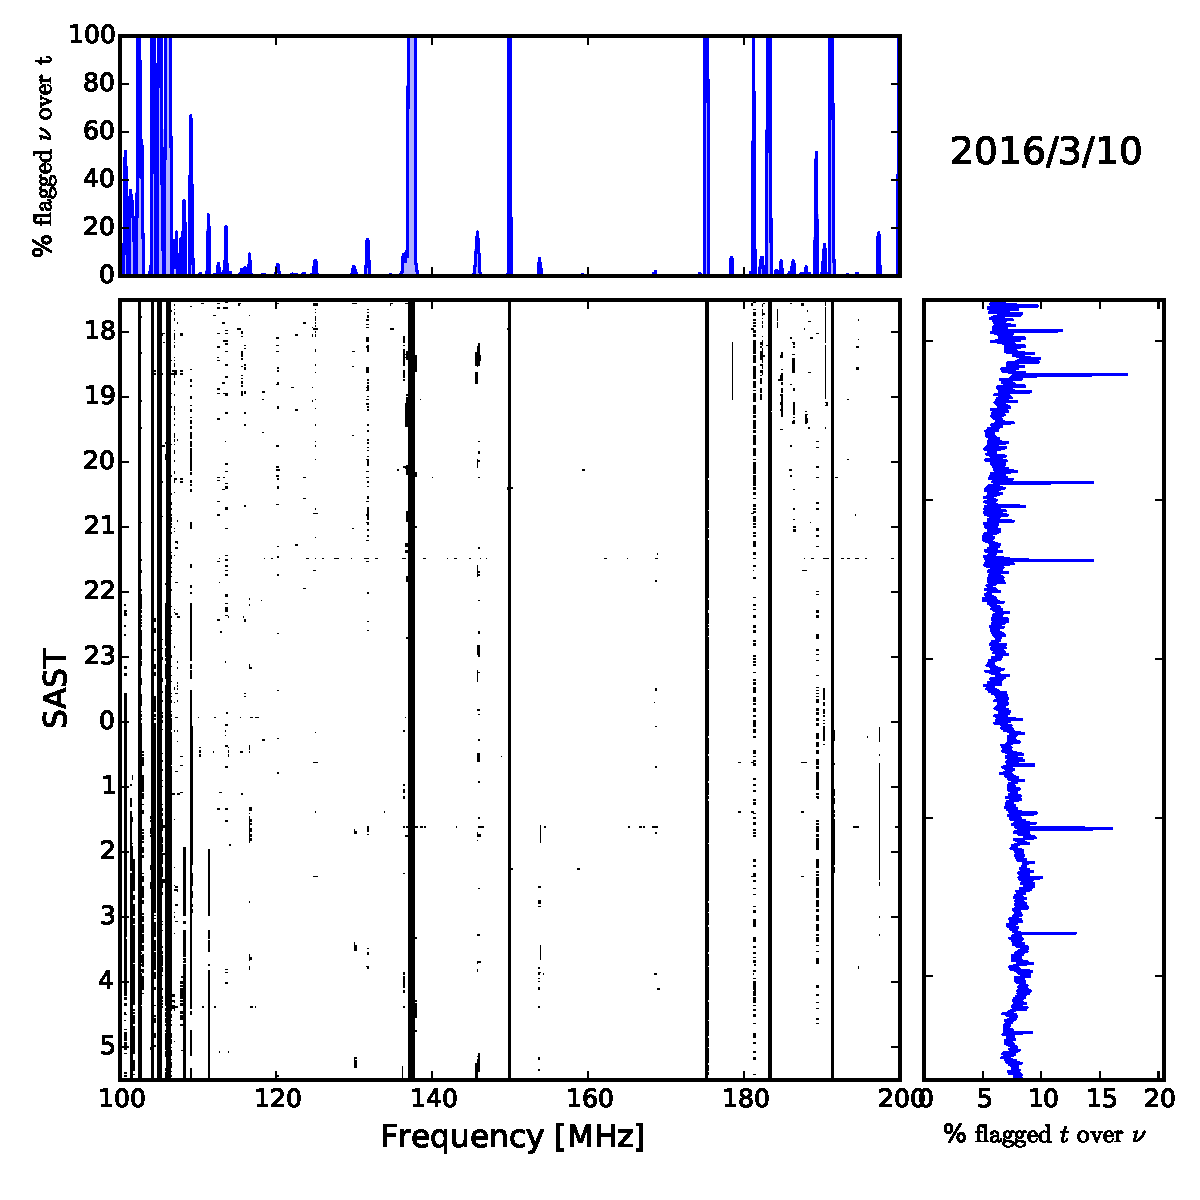
\includegraphics[width=0.45\textwidth]{chapters/data_processing/figures/RFI_HH_wf_tzoom.pdf}
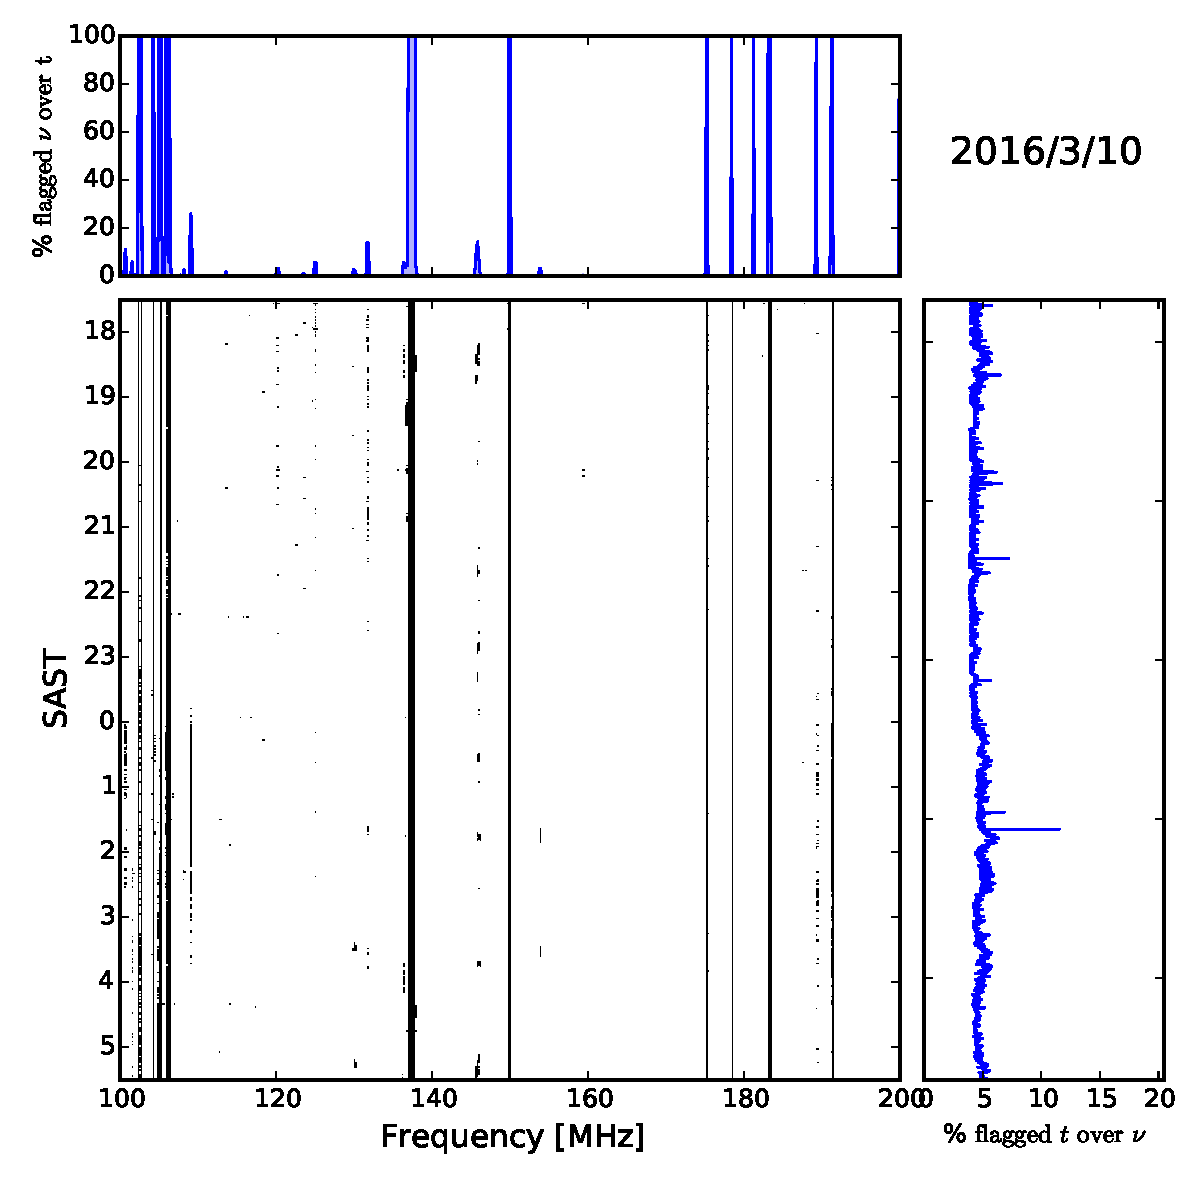
\includegraphics[width=0.45\textwidth]{chapters/data_processing/figures/RFI_PH_wf_tzoom.pdf}
\caption[RFI flag waterfalls of frequency vs. South Africa Standard Time for the HERA Hex and PAPER Hex.]{RFI flag waterfalls of frequency vs. South Africa Standard Time for the HERA Hex (\textit{left}) and PAPER Hex (\textit{right}). The top panels show the average over time (identical to Figure~\ref{fig:rfi_spec_hex_comparison}), while the right panels show the average over frequency.}
\label{fig:rfi_hex_waterfalls}
\end{figure}

\subsubsection{Comparison PAPER-128 stacked flags}
Section~\ref{subsec:rfi_paper128} presented RFI flags stacked over 150 days of observations. This method washed-out single events that effect analysis on a single-night basis, but was sensitive to repeatedly offending frequencies. Due to the PAPER-128 analysis pipeline, many channels were automatically flagged (particularly large portions of the band edges), which artificially boosted the average flagging per time and did not allow for closer inspection of the ends of the band. There was some evidence of broadband emission (see Figure~\ref{fig:rfi_psa128_waterfall}) but the band was largely free of RFI in the middle of the night. Obviously, the data presented in this section shows a less-clean band, but it also only concentrated on a single night's data, so it may be that IDR1 was conspicuous compared to an `average' night of observations.

Traits shared between the two analyses were:
\begin{itemize}
\item Aircraft communications disrupting data until around local midnight.
\item ORBCOMM spilling out of it's band.
\item VHF TV frequencies emitting throughout the night in the high end of the band.
\end{itemize} 

Table~\ref{tab:rfi_herahex} highlighted many frequencies seen by HERA and not by PAPER-128. Again, given the fact that flags were stacked and averaged in Section~\ref{subsec:rfi_paper128}, these may not have been `new', but they could have been. Particularly conspicuous were the emissions in the aeronautical radionavigation band.

\subsubsection{Discussion}
\label{subsubsec:rfi_herapaper_conc}

I have presented a first look at RFI in HERA-19 Commissioning data. Probably due to the height of the receiving element on HERA versus PAPER dipoles, much more RFI was apparent, especially on the low and high ends of the band. Luckily, the EoR band was largely clean of RFI, except for an emitter at about 154~MHz, which could have corresponded to single-frequency mobile phone communications. Such communications are officially banned in the SKA Radio Quiet Zone \citep{SAKRQZ}, which HERA is in the center of.

Only looking at a single night of RFI flags limited the predictive power of this study. More data will be required to establish whether or not this is level of RFI was `normal'. Broadband RFI bursts require closer investigation.

Efforts to extend the HERA band to lower and possibly higher frequencies are currently under way. The FM radio band extends to around 65~MHz, while the VHF TV band extends to around 230~MHz, so the RFI environment should be a consideration for these efforts.

Meanwhile, I note that the RFI flagging routine used here, {\tt xrfi\_simple}, is indeed `simple'. More advanced RFI flagging algorithms such as {\tt AOFlagger} \citep{AOflag} should be tested in later studies.

\section{Quality Assurance Metrics}

Throughout reduction of PAPER-128 data, we found a number of ways for data to become corrupted, including failure of analog or digital components, incorrect cable connections, or improper feed installation. Many of these can cause failure of redundant calibration algorithms that are sensitive to non-redundancies within an array. In the case of a real-time calibration pipeline, such as the one implemented for HERA, it is essential to have quickly-generated metrics to assess the overall health of the array. Much of the heritage of PAPER-128 data processing is present in the HERA Real Time Calibration Pipeline (RTC; {\color{red} Ali et al. (in prep.)}).

\subsection{Mean Amplitude Flagging}
\label{subsec:meanvij}

The most critical and likely failure that an antenna could have was malfunctioning electronics losing power and temporarily `killing' it.
This failure mode was characterized with unusually low signal coming from the antennas, causing the visibilities
associated with that antenna to have much lower than average amplitude. This
leads to the definition of the mean visibility metric for antenna ${i}$:

\begin{equation}
    M_{i} = \frac{ \sum_{j,\nu,t} {|V_{ij}|} }{N-1}
\label{eq:meanvij}
\end{equation}

where $V_{ij}$ is the visibility for the baseline involving antennas $i$ and
$j$, $N$ is the number of antennas in the array, and the sum is taken over all
antennas $j$ ($i \neq j$), times, and frequencies. When $M_{i}$ is compared across the array, 
it can reveal antennas with anomalously low signal to noise.

Erroneously cross-polarized antennas were ones where the feed was rotated 90 degrees, or the
cables were swapped for the two polarizations along the signal path (such a failure mode
could be expected for a large array under active construction). This caused
the linear polarization visibilities ($EE$ or $NN$) to have a lower amplitude or
correlation relative to the cross-polarizations ($EN$ and $NE$). While these could appear to be dead antennas, 
the cross-polarization visibilities would show that one of the antennas in a given
visibility is cross-polarized.

We defined the mean visibility cross-polarization metric as 

\begin{equation}
P_{i} = \frac{M_{i}^{NE} + M_{i}^{EN}}{M_{i}^{NN} + M_{i}^{EE}},
\label{eq:meancrossvij}
\end{equation}

where $M_{i}$ is defined in Equation~\ref{eq:meanvij} and are calculated for
all the polarization pairs. If $P_{i}$ is larger than some threshold, then
antenna ${i}$ may be cross-polarized. This method is effective when applied
to long baselines, but for the shortest baselines in HERA, large-scale astrophysical polarization
\citep[e.g.][]{Lenc.16} is observed by in all the instrumental visibilities 
(since, for example, the $NN$ visibility is equal to the sum of the 
Stokes I and Q visibilities). This brings $P_{i}$ closer to unity
for any antenna $i$.

\begin{figure}
\centering
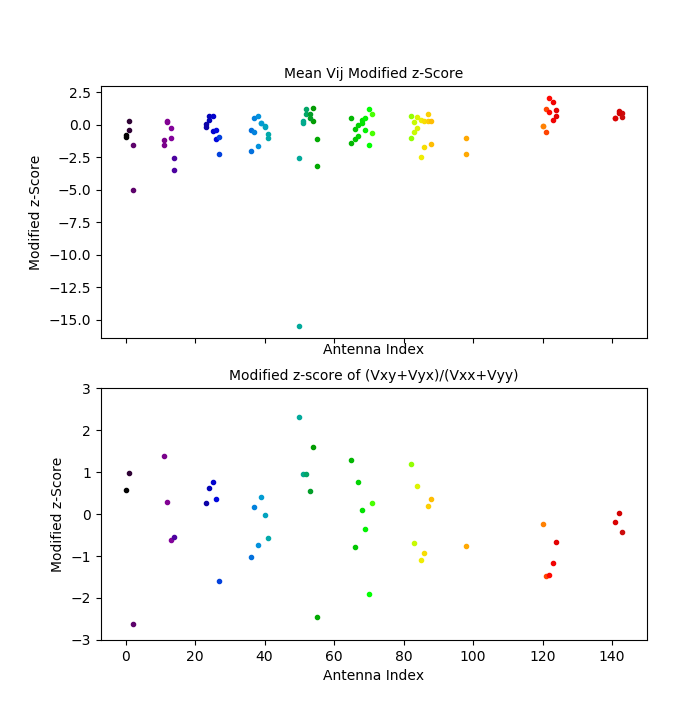
\includegraphics[width=0.7\textwidth]{chapters/data_processing/figures/metrics.png}
\caption[An example of the mean amplitude flagging metrics on exercised on HERA-47 data.]{An example of the mean amplitude flagging metrics on exercised on HERA-47 data. The top panel shows the mean amplitude flagging metric $M_i$, and the lower panel shows the cross-polarization metric $P_i$. The $E$ feed of antenna 50 shows at $\sim$15$\sigma$ deviation, causing it to be flagged from further processing.}
\label{fig:data_metrics}
\end{figure}

Figure~\ref{fig:data_metrics} shows the application of the metrics described above to raw HERA-47 data in the RTC system. Note that we plotted the modified \textit{z}-score and not
the raw metric. Traditionally the \textit{z}-score is defined as the deviation from the
mean divided by the standard deviation, and is a method to detect outliers.
However, since our metrics were not necessarily normally-distributed, we use the
modified \textit{z}-score defined as 

\begin{equation}\label{eqn:modifiedzscore}
    MZ_{i} = 0.6745\frac{|x_{i} - \tilde{x}|} {MAD},
\end{equation}

where $x_{i}$ is some data point (in our case this was a metric),
$\tilde{x}$ is the median of ${\{x_{i}\}}$, and MAD is the median absolute
deviation. \cite{Iglewicz.10} recommend that modified
\textit{z}-scores with an absolute value greater than 3.5 should be flagged as outliers.
In the analyses shown in Figure~\ref{fig:data_metrics}, we took the cut-off to be 5, to account for greater acceptable
variation in our metrics.

The top panel of figure \ref{fig:data_metrics} shows the modified \textit{z}-score for
the mean visibility metric as a function of antenna number.
Antenna 50E (East-West polarization) was a $\sim$15$\sigma$ outlier, indicating a problem
with amplification along the signal chain. Upon further inspection,
antenna 50E was shown to exhibit strange behavior, dropping in and out of the signal chain. Further
investigation is needed to know the root cause of this misbehavior. 

The bottom row of figure \ref{fig:data_metrics} shows the modified \textit{z}-score for the cross
polarization metric as a function of antenna number. There were no modified
\textit{z}-scores outside of the [-5,5] range, indicating that there were no cross polarized
antennas. Further inspection of the raw visibility data validated this finding.

\subsection{Flagging on {\tt omnical} $\chi^2$}

We developed a metric that identified days of PAPER-128 observations with poor overall {\tt omnical} $\chi^2$ values. Using the median of the $\chi^2$ values in the EoR band (channels 100--160; 150--180\,MHz), over all days of observation, we flagged days that exceeded the average of the median by one standard deviation from the mean. Figure~\ref{fig:data_chisq_flagging} shows an example of this flagging method used on the latter half of the first PAPER-128 observing season. Clearly, there were just a few JDs that had exceptionally high $\chi^2$ values. Our metric captures almost all of these outliers -- the possible exceptions being JDs 2456717 and 2456718.

\begin{figure}
\centering
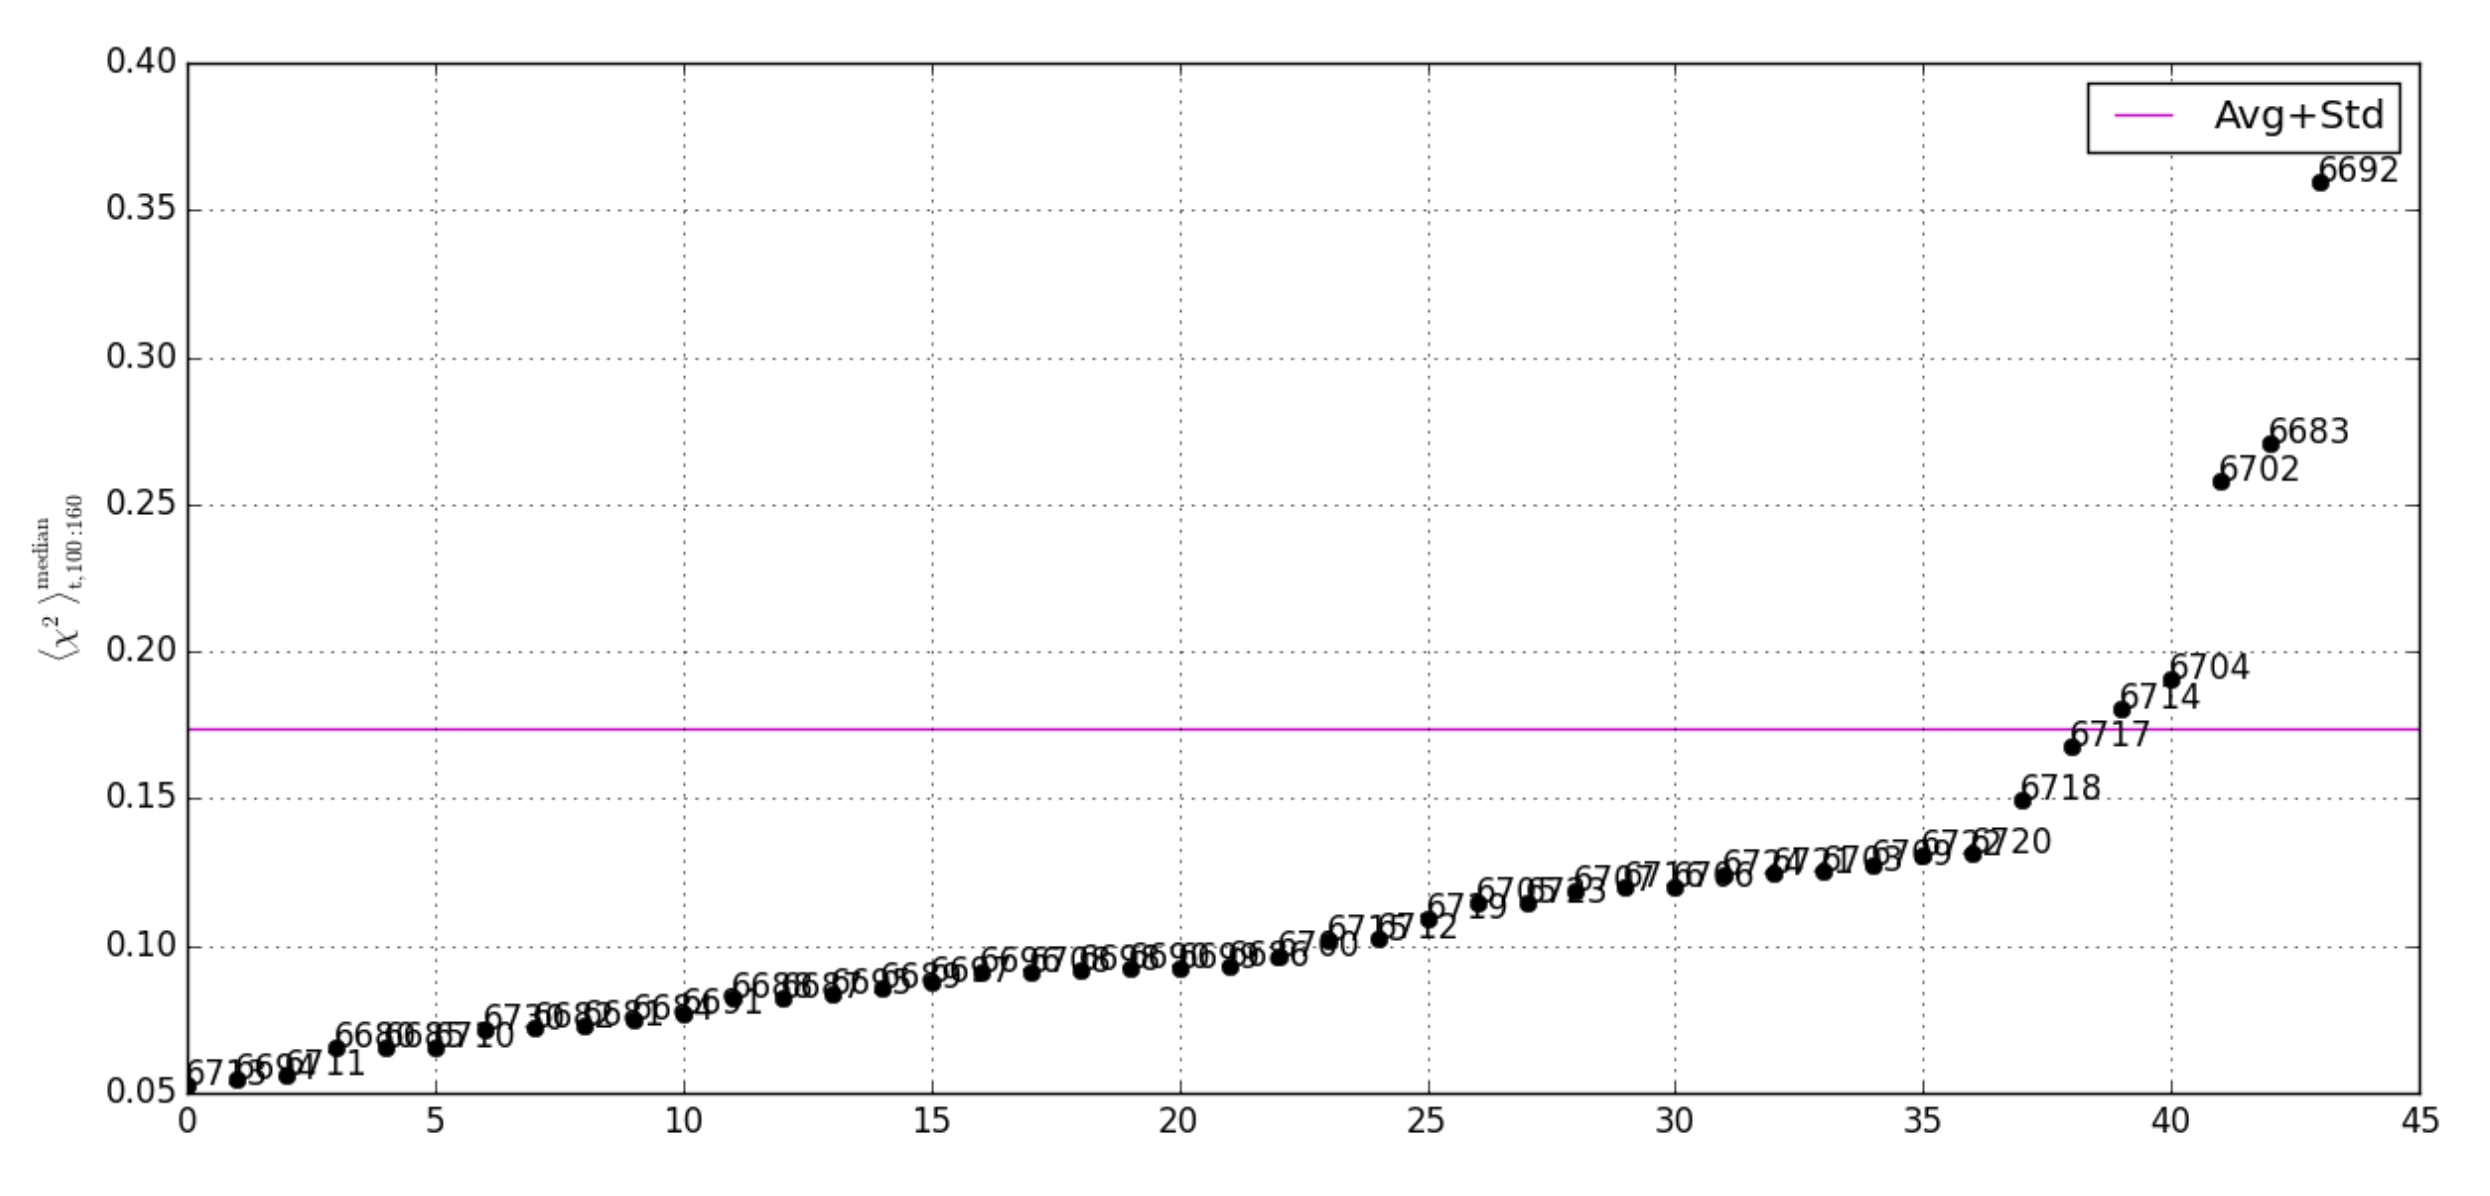
\includegraphics[width=0.7\textwidth]{chapters/data_processing/figures/chisq_flagging.png}
\caption[Flagging Julian Dates based on the median {\tt omnical} $\chi^2$ values in the 150--180\,MHz band.]{Flagging Julian Dates (JDs) based on the median {\tt omnical} $\chi^2$ values in the 150--180\,MHz band. Shown in pink is the flagging boundary. The JD labels have been abbreviated to drop the `245' prefix that they all share. Clearly, there are just a few JDs that have exceptionally high $\chi^2$ values.}
\label{fig:data_chisq_flagging}
\end{figure}

The {\tt omnical} software also provides $\chi^2_a$ values for each antenna $a$ -- that is, how much each antenna contributed to the overall non-redundancy of the array. The above sigma-clipping metric was applied to $\chi^2_a$, and was able to identify the same bad antennae using the mean amplitude flagging metric described in Equation~\ref{eq:meanvij}.

%
% compression -- DDR algorithm & software overview -- DONE
% PAPER-128 RFI memo -- DONE
% HERA RFI memo -- DONE
% PAPER QA
%
\chapter{Polarimetric Calibration}
\label{chapter:polcal}

Hypothetically, integrating over long observing seasons should average-down the noise in the EoR window, allowing for the study of the EoR without the risk of foreground contamination. However, the wedge-window paradigm arises due to the chromaticity of the interferometer as well as the signal. Spectral structure can be imparted to interferometric visibilities by the frequency evolution of the antenna beam and by calibration. Spectral structure can also be induced on otherwise-smooth foregrounds via Faraday rotation of polarized foregrounds. In of itself Faraday rotation is not a problem, since {\sc hi} emission should be largely unpolarized, but errors in calibration and beam deconvolution can leak polarized signal into unpolarized visibilities \citep[e.g.][; Chapter~\ref{chapter:interferometry}]{TMS}.

Interferometers with $N$ antennae that are sensitive to $N_{\rm pol}$ polarizations will generate $N_{\rm pol}N(N-1)/2$ visibilities per time-frequency sample, defined as:

\begin{eqnarray}
V_{ij,pq}(\nu, t) = g^*_{p,i}(\nu,t) g_{q,j}(\nu,t) \exp(-2\pi\nu \tau_{pq}) \times \nonumber\\
\int {\rm d}\Omega A_{pq}(\nu, \hat{s}) S_{P}(\nu, \hat{s}) \exp(i \vec{b}_{ij}\cdot\hat{s} \nu/c)
\end{eqnarray}

where $p,q \in x,y$ denote instrumental polarizations, i.e. the response to signal projected into the North-South direction or the East-West direction, or whichever direction the dipole arms of the instrument are oriented; $i,j$ refers to two antennae with baseline vector $\vec{b}_{ij}$, $S_{P}(\nu, \hat{s})$ is the sky temperature for Stokes parameter $P$, and $A_{pq}(nu, \hat{s})$ is the spatial sensitivity of the instrument to $S_{P}$ (projected into the instrumental basis). Outside the integral are three direction-independent variables that must be calibrated: the complex gain of each dipole arm $g_{p,i}(\nu,t)$ and the phase between dipole arm $p$ and $q$, $\tau_{pq}$. For $p=q$, $\tau_{pq}=0$.

All the above presents a data processing challenge: these visibilities must be precisely calibrated over long observing seasons to ensure that the cosmological signal is not averaged away by calibration errors and not contaminated by spectral structure. One way of overcoming part of this challenge is to construct large arrays of redundantly-spaced elements. The redundancy of the visibilities of such an interferometer allows the gain terms to be solved-for precisely by least-squares minimization algorithms \citep{Liu.10}. In Section~\ref{sec:polcal_redcal}, I explore the implications of implementing full-polarization redundant calibration on PAPER-128 data. However, redundant calibration is not the only tool radio astronomers posses that can be used to obtain precise calibration solutions. In Section~\ref{sec:polcal_imagecal}, I present a basic implementation of full-polarization image-based calibration on data from the PAPER-32 polarized imaging array.

\section{Redundant Calibration}
\label{sec:polcal_redcal}

Unpolarized redundant calibration has been pursued by the Donald C. Backer Precision Array for Probing the Epoch of Reionization (PAPER; \citet{Parsons.10}), the Hydrogen Epoch of Reionization Array (HERA; \citet{deBoer.17}) and part of the Murchison Widefield Array (MWA; \citet{Tingay.13}). For EoR studies this has the advantage of being able to average-down noise in the EoR window once all redundant visibilities are calibrated, for potentially very high signal-to-noise measurements of narrow regions of \textit{k}-space. However, it sacrifices $uv$-coverage, leading to poor imaging capabilities.

Redundant calibration of low-frequency interferometers has been demonstrated by \citet{Zheng.14} with the MIT EoR experiment, \citet{Parsons.14, Jacobs.15, Ali.15}  and {\color{red} Kolopanis et al. (2018)} with PAPER and {\color{red} Li et al. 2017} with part of the MWA. All of these studies calibrated linearly-polarized instrumental visibilities. 

\citet{Moore.17} used the same calibration parameters as \citet{Parsons.14} and \citet{Jacobs.15}, but also solved for a single value of $\tau_{pq}$ for the observing season, since their analysis was for cross-polarized visibilities also. These PAPER studies took linear combinations of instrumental visibilities to form `pseudo-Stokes' visibilities (e.g. \citet{TMS}, \citet{Moore.13}). In this Chapter, we use the notation and convention

\begin{equation}
\left(\begin{array}{c}
V_{I}\\
V_{Q}\\
V_{U}\\
V_{V}\end{array} \right)
= \frac{1}{2}
\left( \begin{array}{cccc}
1 & 0 & 0 & 1 \\
1 & 0 & 0 & -1 \\
0 & 1 & 1 & 0 \\
0 & -i & i & 0 \end{array} \right) 
\left(\begin{array}{c}
V_{xx}\\
V_{xy}\\
V_{yx}\\
V_{yy}\end{array} \right) 
\label{eq:polcal_pseudo-stokes}
\end{equation}
for these quantities.

As noted above, the spectrally-structured HI emission from the EoR should only be detected in $V_{I}$, but fractions of Faraday-rotated (spectrally structured) $V_{Q}$ and $V_{U}$ are capable of leaking into $V_{I}$ via calibration errors and intrinsic properties of the complex beam. Short of detecting the polarized power spectrum of $V_{Q}$ and $V_{U}$, which may be at levels beneath the EoR signal, we require confidence that we are accurately calibrating our data to prevent as much leakage as possible into $V_{I}$. 

At these low frequencies and inherently large scales probed by modern instruments, the Stokes V sky appears to be empty. Indeed, \citet{Patil.17} used the spherical power spectra of their Stokes V images as a proxy for the thermal noise power spectrum. In wedge-space, one test of polarimetric calibration is therefore to see how close to thermal noise $V_{V}$ is. 
\citet{Kohn.16} observed a direction-independent bias in $V_{V}$, but that study implemented a \citet{Moore.17}-style polarimetric calibration of $\tau_{pq}$, solving for a single value across the array, which could indeed lead to a direction-independent bias (but was more powerful than not calibrating it at all; see their Figure 5).

In Section, we explore different schemes of redundant calibration which include polarization. We present three different calibration schemes, all based around the {\sc omnical}\footnote{\url{https://github.com/HERA-Team/omnical}} package \citep{Zheng.14}, and compare their uses and shortcomings. We structure the discussion as follows: in Section~\ref{sec:polcal_math} we give a mathematical overview of the least-squares minimization algorithms implemented for the different calibration schemes and show basic simulations of each algorithm in action. We describe the real data used to test the calibration schemes, and the results of those tests, in Sections~\ref{sec:polcal_data} and \ref{sec:polcal_results}, respectively. We discuss our findings and conclude in Section~\ref{sec:polcal_disc}.

\subsection{Mathematical Overview}
\label{sec:polcal_math}

In this section we briefly describe the fundamental steps of the redundant calibration scheme implemented in {\sc omnical}. For a more thorough discussion of the algorithm, see \citet{Wieringa.92}, \citet{Liu.10}, \citet{Zheng.14} and \citet{Dillon.17}. 

\subsubsection{Redundant calibration with {\sc omnical}}

We can express visibilities for baseline separation $|i-j|$, polarization $pq$ as a system of equations, of form

\begin{equation}
V_{ij,pq} = g^*_{p,i} g_{q,j} V_{|i-j|,pq} + n_{ij}
\label{eqn:vismdl}
\end{equation}

where we have dropped the frequency and time dependence; this is true for every time-frequency sample. This system is overdetermined for a highly redundant array configuration. We assume that all polarizations have the same noise statistics for noise $n_{ij}$. An initial estimate for the least-squares fit can be obtained by solving the linearized equation in logarithmic space (termed \textit{logcal})

\begin{equation}
\log V_{ij,pq} = \log g^*_{p,i} + \log g_{q,j} + \log V_{|i-j|,pq}
\label{eqn:logcal}
\end{equation}

which can constrain the parameter space, but produces biased results since noise is additive in linear space. Taylor expanding Equation~\ref{eqn:vismdl} around the estimated values (denoted with bars) for each parameter as found by \ref{eqn:logcal} grants a system of linearized equations (termed \textit{lincal})

\begin{eqnarray}
V_{ij,pq} = \bar{g}^*_{p,i} \bar{g}_{q,j} \bar{V}_{|i-j|} + g^*_{p,i} \bar{g}_{q,j} \bar{V}_{|i-j|} + \nonumber\\
 \bar{g}^*_{p,i} g_{q,j} \bar{V}_{|i-j|} + \bar{g}*_{p,i} \bar{g}_{q,j} V_{|i-j|}
\end{eqnarray} 

which can be solved iteratively, minimizing the least-squares statistic $w$

\begin{equation}
w^2 = \sum_{\rm{all } i \neq j} \sum_{p,q \in x,y}\frac{|V_{ij,pq} -  g^*_{p,i} g_{q,j} V_{|i-j|,pq}|^2}{\sigma_{ij}}.
\label{eq:polcal_w2}
\end{equation}

\subsubsection{Including polarization in redundant calibration}
\label{subsec:calSchemes}

We test three different calibration schemes for polarization. 

\begin{itemize}
\item Use {\sc omnical} separately on the two linearly polarized visibilities $V_{xx}$ and $V_{yy}$ to obtain independent estimates for all gain terms, and apply those gains to all four instrumental polarizations of visibilities. We will refer to this scheme as \textit{2pol} calibration. 

\item Include all four instrumental polarizations in the least-squares statistic. This means that, for example, information on the $g_{x,i}$ term will come from $V_{xx}$ and $V_{xy}$. This will be referred to as \textit{4pol} calibration. 

\item Use a scheme in which the cross-polarized visibilities $V_{xy}$ and $V_{yx}$ share values of the model visibility $V_{|i-j|,pq}$. This means that we are minimizing the value of $V_{yx} - V_{xy}$ during calibration; effectively minimizing the pseudo-Stokes V visibility. There is validity to assuming the pseudo-Stokes V visibility to be noise-like, as discussed above. We refer to this calibration scheme as \textit{4pol+minV} calibration.
\end{itemize} 

\subsubsection{Degeneracies}
\label{subsubsec:degen}

One virtue of {\sc omnical} is that it can calibrate all antennas relative to one another without reference to an explicit sky model. However, this results in known degeneracies in the minimization of $w^2$ that cannot be resolved with {\sc omnical} and must be fixed afterwards with absolute calibration of the whole array using external information. The number of degeneracies is equal to the number of zero eigenvalues that arise in the linearized $w^2$ minimization algorithm. For a single polarization, there are 4 degenerate modes, which can be interpreted physically as overall amplitude, overall phase, phase tilt, and phase tip. Phase tilt and tip can be interpreted as a two-dimensional phase slope across the array. It is clear that these factors to not affect the product $g^*_{p,i}(\nu,t) g_{q,j}(\nu,t)V_{ij,pq}(\nu, t)$ (and we again refer the reader to \cite{Dillon.17} for a comprehensive description):

\begin{itemize}
\item Overall amplitude: $g_{p,i} \rightarrow A g_{p,i}$ and $V_{ij,pq} \rightarrow V_{ij,pq}/A^2$.
\item Overall phase: $g_{p,i} \rightarrow g_{p,i}e^{i\phi}$
\item Two-dimensional phase slope: for a co-planar array, define a phase vector $\vec{\Upsilon} = (\Upsilon_X,\Upsilon_Y)$ where $\Upsilon_X,\Upsilon_Y$ refer to Cartesian directions as opposed to polarizations. For an antenna at position $\vec{\upsilon}_i$, and defining $\vec{d}_{ij} = \vec{\upsilon}_i - \vec{\upsilon}_j$, then $g_{p,i} \rightarrow g_{p,i}e^{i\vec{\Upsilon}\cdot\vec{\upsilon}_i}$ and $V_{ij,pq} \rightarrow V_{ij,pq}e^{i\vec{\Upsilon}\cdot\vec{d}_{ij}}$. This is allowed because $\vec{d}_{ij}$ is the same for all redundant visibilities.
\end{itemize}

{\sc omnical} `fixes' the amount that the amplitude degeneracy is able to drift between samples by imposing that the average of the absolute of the gains over the array average to unity. Similar tricks can be played with the other degeneracies to project them into a space that does not adversely effect calibration.

The phenomenon of `degeneracy fixing' in polarized redundant calibration was explored in depth by \citet{Dillon.17}. In that work, they showed how the number of degeneracies changes with polarized calibration scheme, focussing on what we refer to as the \textit{2pol} and \textit{4pol} schemes in this work. We briefly review their results here. 

In the \textit{2pol} scheme, there are the 8 expected redundancies as expected for two independent calibrations; it is as if there are two co-located arrays for $xx$ and $yy$, each with the four degeneracies listed above. However, in the \textit{4pol} scheme, the number of degeneracies is reduced to 6. Introducing $V_{xy}$ and $V_{yx}$ breaks the phase tilt and tip degeneracies per polarization, and leaving a polarization-independent phase tilt and tip. Extending this formalism to the \textit{4pol+minV} scheme\footnote{As explored in the public HERA Memo \#30.}, the number of degeneracies is further reduced to 5. By imposing equality between $V_{xy}$ and $V_{yx}$, the `overall phase' degeneracies per polarization are broken and there remains only a single overall phase for the array.

\citet{Dillon.17} emphasized the importance of understanding how fixing degeneracies can effect the amplitude of noise in redundant calibration solutions. They found that although the number of degeneracies decreased in the \textit{4pol} scheme, $V_{xy}$ and $V_{yx}$ had low enough signal to noise that their inclusion in calibration greatly increased the noise in the gain solutions. Fixing only the 6 degeneracies of that scheme introduced much greater noise amplitude in the calibration solutions. However, fixing the 8 degeneracies from the \textit{2pol} scheme \textit{while still calibrating} with the \textit{4pol} scheme gave almost identical gain solutions. Learning from this, we fix the 8 degeneracies from the \textit{2pol} scheme throughout the rest of this work, independent of the calibration scheme used.

\subsubsection{Expectations from simulation}  

Using the formalism of \cite{Nunhokee.17} and Chapter~\ref{chapter:interferometry}, and the HFSS\footnote{\url{http://www.ansys.com/Products/Electronics/ANSYS-HFSS}} complex voltage simulations of the PAPER beam described therein, we simulated the polarized response of the instrument to an unpolarized sky. That is, we passed a Stokes I - only sky model \citep[][]{GSM.08} over a 30\,m East-West baseline -- the baseline vector of interest for the PAPER experiment \citep{Parsons.14, Jacobs.15, Ali.15, Moore.17}. This meant that whatever was observed in the pseudo-Stokes Q, U and V visibilities could be interpreted as direction-dependent leakage from Stokes I (the expected regime for a single night of observations with PAPER; \citet{Kohn.16}). The 2008 Global Sky Model used for the simulation was primarily diffuse in nature, with the `A-Team' of bright low-frequency sources (Fornax A, Pictor A, etc.) also included. The diffuse nature was appropriate for the fringe profile of a 30\,m baseline. The output of the simulation is shown in Figure~\ref{fig:simvis} with and without the inclusion of an instrumental noise model, with the system noise drawn from \cite{Moore.17}.

\begin{figure}
\centering
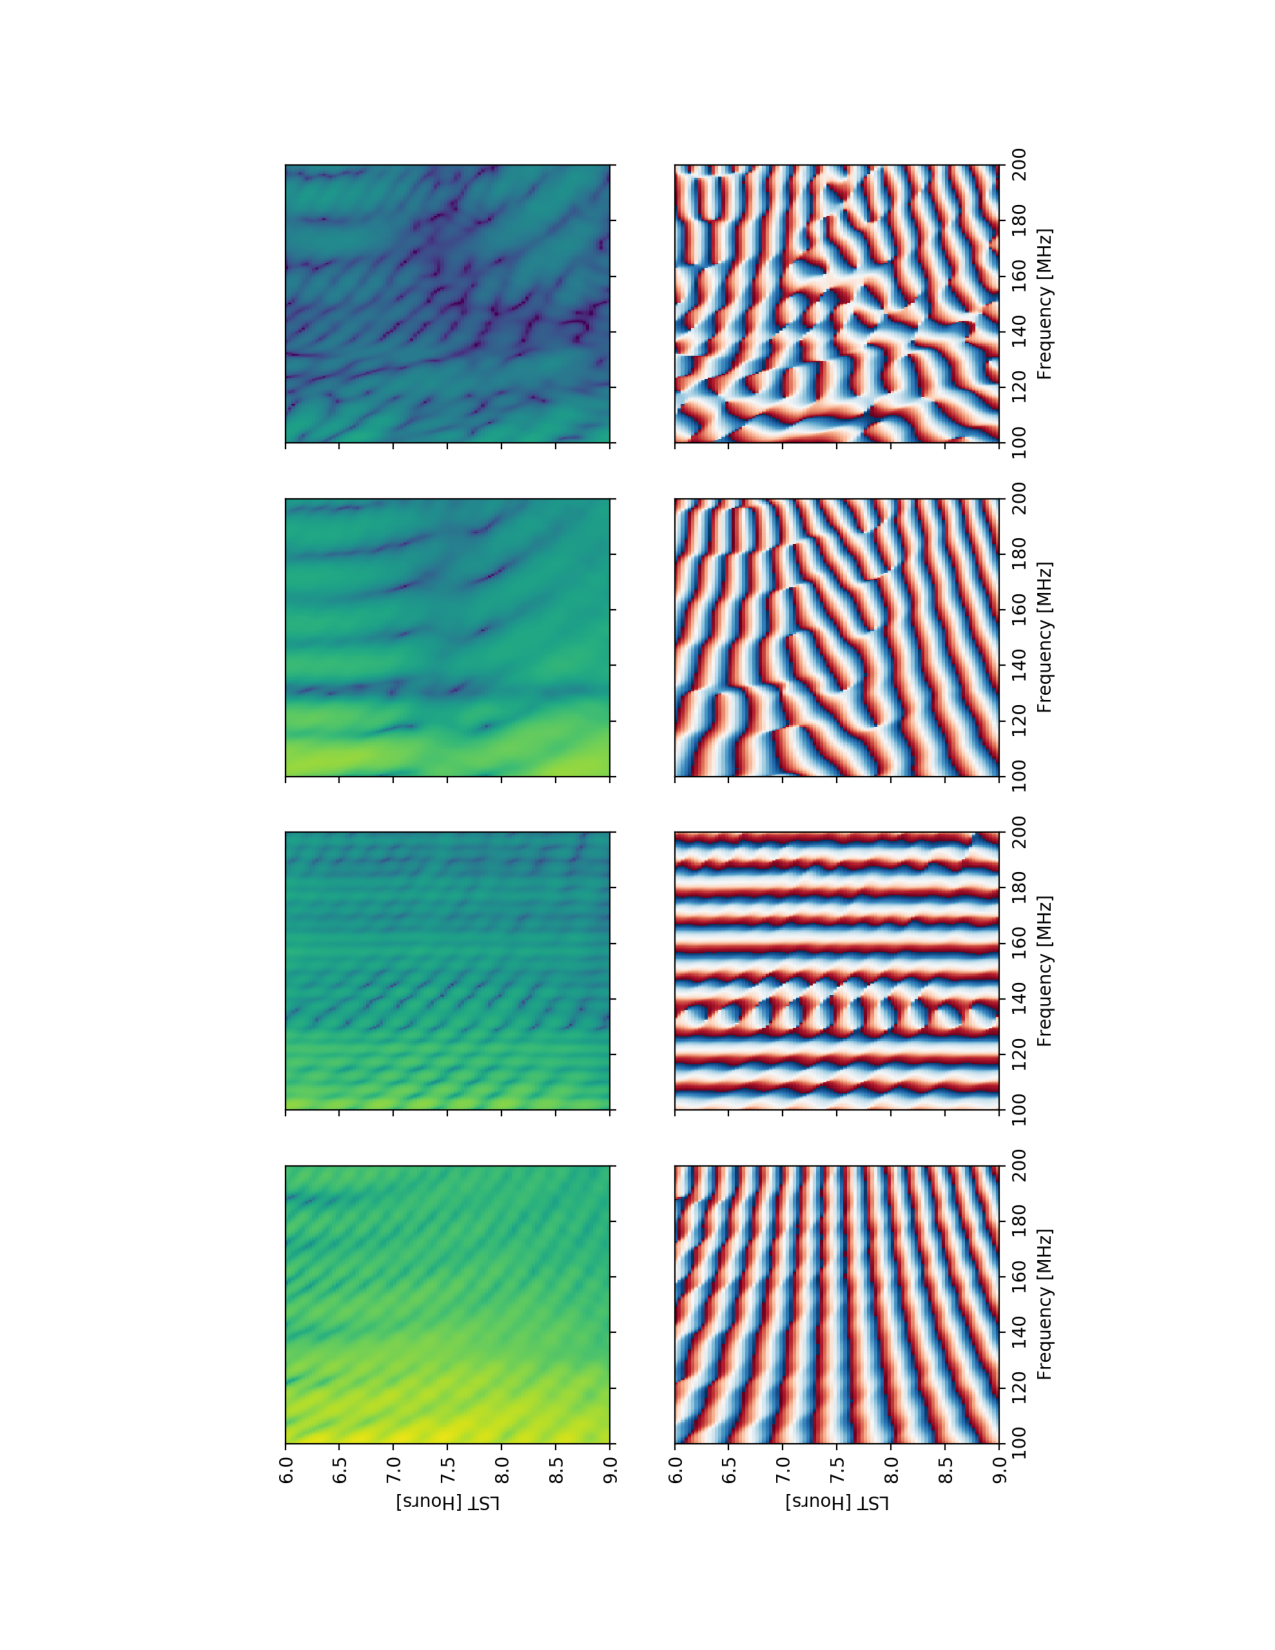
\includegraphics[width=0.6\textwidth, angle=270]{chapters/polcal/figures/sim_nonoise.pdf}
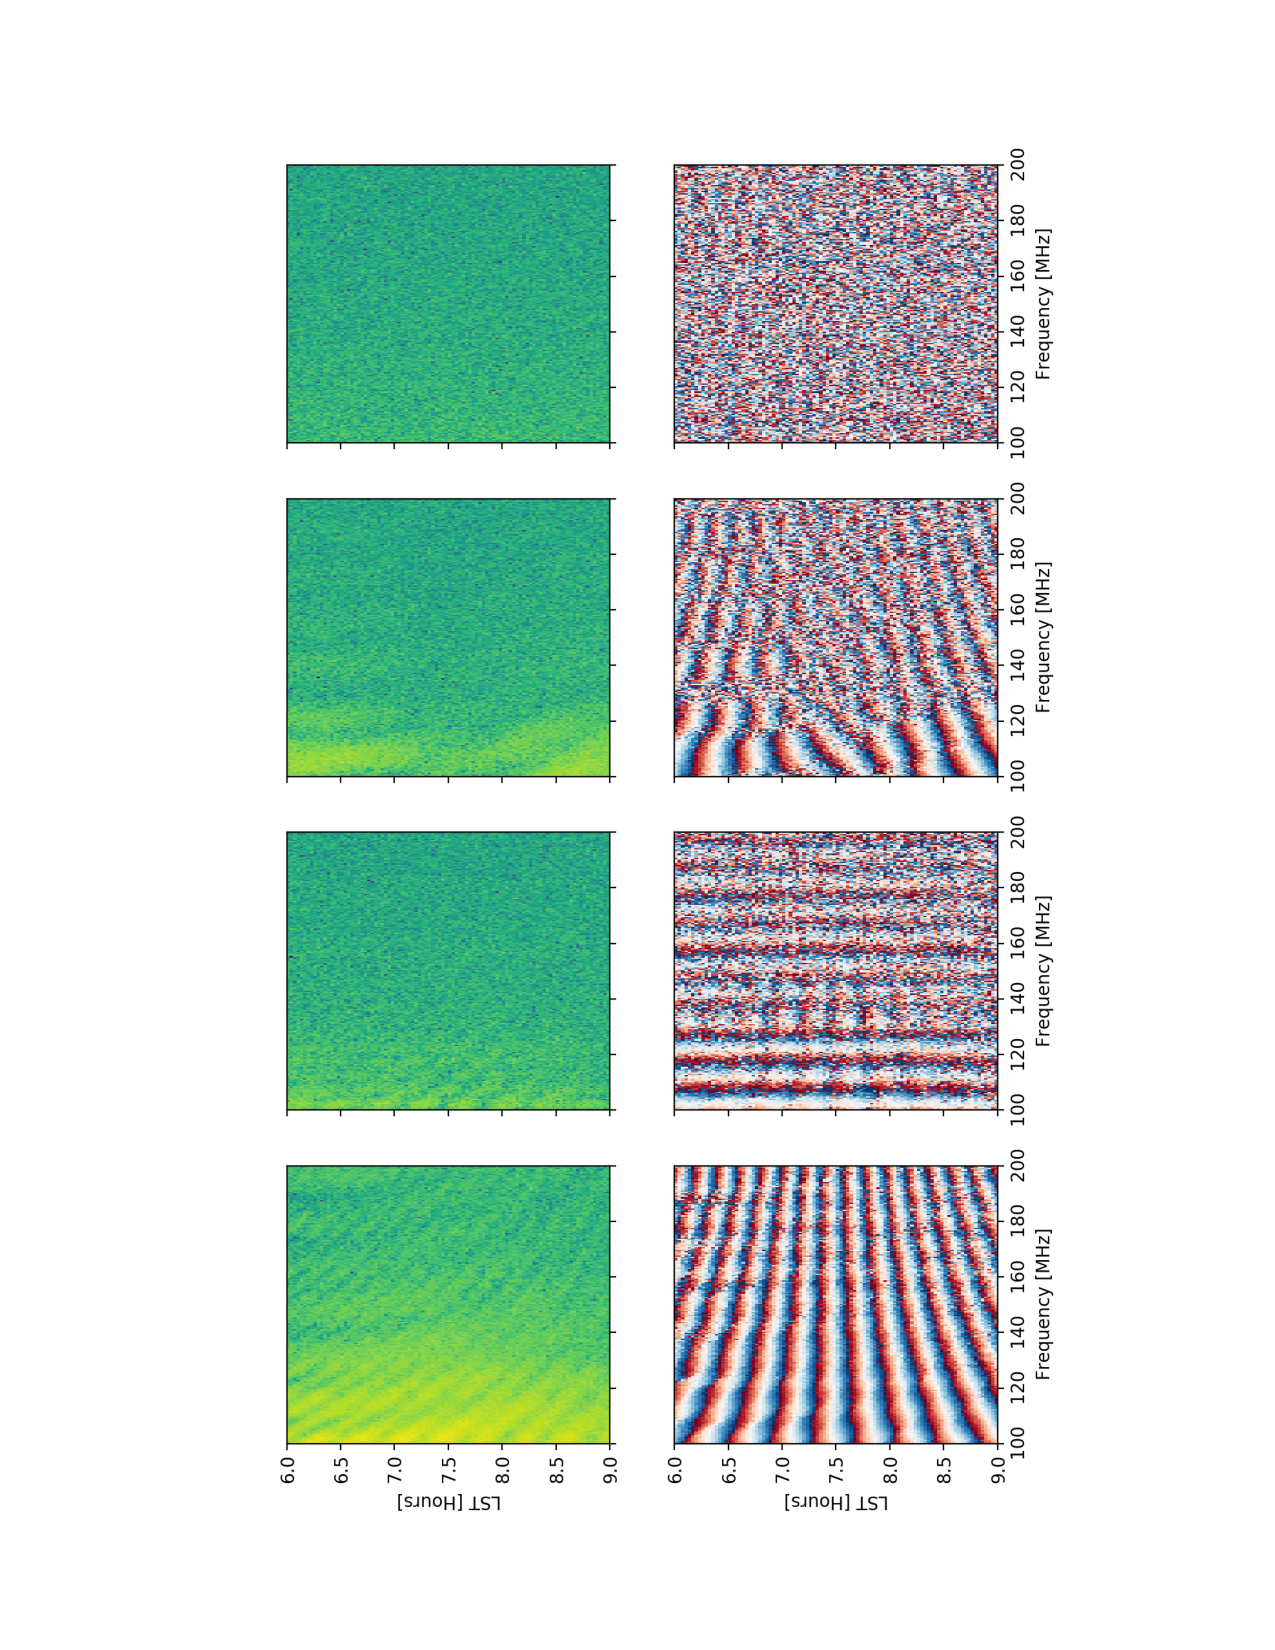
\includegraphics[width=0.6\textwidth, angle=270]{chapters/polcal/figures/sim.pdf}
\caption[Simulations of pseudo-Stokes visibilities,]{Simulations of absolute value (\textit{upper panels}) and phase (\textit{lower panels}) of pseudo-Stokes visibilities (left to right: pseudo-Stokes I, Q, U and V), as measured by a 30\,m East-West PAPER baseline. The upper group shows the noiseless simulation, and the lower shows the same simulation with the addition of a realistic PAPER noise model \citep{Moore.17}. Only a Stokes I sky was used -- all of the structure seen in $V_Q$, $V_U$ and $V_V$ can be attributed to direction-dependent leakage.}
\label{fig:simvis}
\end{figure}


\subsection{Data Processing}
\label{sec:polcal_data}

We tested these different calibration schemes on one night (JD 2456680.20 -- .65; January 22nd-23rd 2014; 6pm -- 6am South African Standard Time; Local Siderial Time 2 -- 13.5 hours) of PAPER 128-element observations. The PAPER-128 signal chain and full observation season results will be discussed in forthcoming publications, but we will provide a brief overview here. 

PAPER-128 consisted of 128 dual-polarization dipole receivers, 112 of which are arranged in a highly-redundant configuration, and the rest placed as in- and outriggers to the array in order to improve \textit{uv}-coverage; see Figure~\ref{fig:polcal_realarray}. Since all dipole arms were oriented North-South (`x') and East-West (`y'), \textit{xy} and \textit{yx} correlations have very low signal-to-noise compared to \textit{xx} and \textit{yy}.

All visibilities were RFI flagged using {\sc python} scripts from the {\sc aipy}\footnote{\url{https://github.com/HERA-Team/aipy}} library. These took the derivative of the frequency axis of all baselines associated with a given antenna and flagged any frequencies with a derivative 6$\sigma$ above the mean, per integration. We took the union of all baseline flags and applied them to the data. The 5\,MHz on both band-edges were always flagged. Compression proceeded as described in Appendix A of \cite{Parsons.14}, filtering to critical Nyquist sampling rates for the longest (300\,m) baseline of 493 kHz along the frequency axis (203 channels) and 42.9\,s along the time axis. 

\begin{figure}
\centering
\includegraphics[scale=0.5]{chapters/polcal/figures/gridlayout.png}
\caption[Arrangement of the PAPER-128 array.]{Arrangement of the PAPER-128 array. Antennae determined to be malfunctioning are shown with red crosses and were excluded from analysis.}
\label{fig:polcal_realarray}
\end{figure}

After RFI flagging and compression, \textit{xx} and \textit{yy} visibilities were checked for erroneous behavior including 2$\sigma$ deviations from the median in number of RFI flags and mean visibility amplitude. Antennae exhibiting these behavior were excluded from further analysis (and are shown with red crosses in Figure~\ref{fig:polcal_realarray}). If an antenna qualified as `bad' in one polarization, it was excluded in all of them. Also note that we could only calibrate the 112 antennae in the redundant grid using {\sc omnical}.

For the least-squares fit to converge at the \textit{logcal} stage of calibration, visibilities cannot exhibit phase-wraps, since the system of equations solved at this stage are insensitive to additive offsets of $2\pi$ in their imaginary parts (\textit{lincal} will be able to re-insert these as required; \citealt{Liu.10}). Therefore we had to flatten the phases on all visibilities prior to any implementation of {\sc omnical}. We were able to do this redundantly without reference to the sky; taking the ratio of redundant (uncalibrated) visibilities together and averaging over time, defined as:

\begin{equation}
\mathcal{V}(\nu) = \langle V_{ij, pq}(\nu,t)V^*_{kl, pq}(\nu,t) \rangle_t .
\label{eq:Vijratio}
\end{equation}

Because this is the ratio of two nominally-redundant visibilities (i.e. baselines $ij$ and $kl$ belong to the same redundant group with model visibility $V_{|i-j|,pq}$), and the measurements are not yet calibrated, we can expand Equation~\ref{eq:Vijratio} as

\begin{equation}
\mathcal{V}(\nu) = \langle g^*_{p,i}g_{q,j}g_{p,k}g^*_{q,l} |V_{|i-j|,pq}|^2 \rangle_t .
\end{equation}
Writing the complex gains as $g_{p,a}=G_{p,a} e^{-i\nu\tau_{p,a}}$ for antenna $a$, we can reduce the product of gain-amplitudes and the squared visibility into some frequency-dependent function, and an exponential product of gain phase terms

\begin{equation}
\mathcal{V}(\nu) = K(\nu)\exp\left(i\nu (\tau_i - \tau_j - \tau_k + \tau_l)\right) .
\end{equation}
A Fourier transform along the frequency axis (which we term a \textit{delay transform}; \citealt{Parsons.12a}) of $\mathcal{V}(\nu)$ gave a function that was sharply-peaked at a given delay

\begin{equation}
\tilde{\mathcal{V}}(\tau) = \tilde{K}(\tau)*\delta_D\left(\nu (\tau_i - \tau_j - \tau_k + \tau_l)\right).
\end{equation}
We can define a variable as the maximum of the above function:

\begin{equation}
\mathcal{T}_{ijkl}(\tau) = {\tt max} | \tilde{\mathcal{V}}(\tau) |,
\end{equation}
which will occur at value 

\begin{equation}
\tau = \tau_{\rm max} = \nu (\tau_i - \tau_j - \tau_k + \tau_l).
\end{equation}
With enough redundant baselines involving antennae $i,j,k$ \& $l$ this is a linearly-solvable set of equations for each value of $\tau$. Multiplying $V_{ij}$ by $e^{-2\pi i \nu (\tau_i - \tau_j)}$ by definition flattened the phase across the band. This method was very sensitive to signal-to-noise, so these initial phase estimates were created with $p=q$; that is \textit{xx} and \textit{yy} visibilities only. The estimates were then applied to all visibilities appropriately. We could then run {\sc omnical} according to each of the schemes described in Section~\ref{subsec:calSchemes}.

\subsection{Results}
\label{sec:polcal_results}

We ran {\sc omnical} using the \textit{2pol}, \textit{4pol} and \textit{4pol+minV} schemes, which granted complex gain values for each antenna feed in the redundant grid. In this Section we chose to concentrate our analysis on the 30\,m East-West spacings used for PAPER power spectrum studies.

\subsubsection{Calibration}

The complex-gains dataset alone was highly multidimensional. We chose to analyze short time- and frequency- averages for these data. For example, the $\langle | g^{\rm 2pol}_{x,a} | \rangle_{t,\nu}$ notation indicates the average of the absolute value of the gain value for antenna $a$, polarization `x' in the \textit{2pol} calibration scheme. The average was over 10 minutes (the length of a single {\sc miriad} file produced by the PAPER correlator) and a 10\,MHz band running from 145 to 155 MHz (the center of the PAPER band, generally clear of RFI and used for power spectrum analyses).

Figure~\ref{fig:4pol-geo-angle} shows $\langle {\rm arg}( g^{\rm 2pol}_{a} ) \rangle_{t,\nu}$, the average phase of the gain calibration for `x' and `y' polarizations. It very clearly shows the phase-slope degeneracy present for both dipole orientations, sloping in opposite directions. 

\begin{figure}
\centering
\includegraphics[scale=0.5]{chapters/polcal/figures/4pol_geo.png}
\caption[The phase of the complex gain value for the \textit{4pol} calibration scheme.]{The phase of the complex gain value for the \textit{4pol} calibration scheme is shown on the color axis (radians) for the redundant grid. The phase of the `x' gains is shown on the left, and the `y' gains on the right. The phase-slope degeneracy is clear in both panels, as is the fact that the slope is in opposite directions for the two dipole orientations.}
\label{fig:4pol-geo-angle}
\end{figure}

Figure~\ref{fig:diff-gains} shows the differences in `x' gain solutions between calibration schemes. 
The difference between \textit{4pol} and \textit{4pol+minV} was consistently smaller than the difference of either of these with the \textit{2pol} scheme. 

As noted in Section~\ref{subsubsec:degen}, {\sc omnical} tried to fix the average gain amplitude over the array to unity to avoid drifts in the amplitude degeneracy from sample to sample, so we were able compare amplitude calibrations in terms of percentage deviation. The average difference in gain amplitude per antenna between \textit{2pol} and \textit{4pol} was 3.5\%, between \textit{2pol} and \textit{4pol+minV} was 2.9\%, and was 0.7\% between \textit{4pol} and \textit{4pol+minV}. The $\sim$30 degree spread in the differenced phases between the \textit{2pol} scheme and the other two was likely due to different realizations of phase degeneracies between these calibration schemes.

\begin{figure}
\centering
\includegraphics[scale=0.5]{chapters/polcal/figures/dGainHist.png}
\includegraphics[scale=0.5]{chapters/polcal/figures/dAngleHist.png}
\caption[Histograms of differences in the `x' gain calibrations per antenna between calibration schemes.]{Histograms of differences in the `x' gain calibrations per antenna between calibration schemes. Above: difference in absolute value. Below: difference in phase.
For most antennae, absolute value of the gain does not change by large amounts between calibration schemes; most of the change takes place in the phase.
The difference between \textit{4pol} and \textit{4pol+minV} is consistently smaller than the difference of either of these with the \textit{2pol} scheme. This is likely a sign of different realizations of phase degeneracies between calibration schemes.}
\label{fig:diff-gains}
\end{figure}


Figure~\ref{fig:polcal_chisq} shows the sum of $w^2$ values (see Equation~\ref{eq:polcal_w2}) over all antennas in the array for each feed polarization in each of the three calibration schemes. The color scale is logarithmic. Clearly, the \textit{2pol} scheme achieves a much greater level of redundancy in each feed polarization throughout the band. Towards the end of the night, the Galaxy was in the far side-lobes of the PAPER beam and introduces higher sky temperatures, which accounted for the trend in all calibration schemes performing worse towards the end of the night. However, the reason for rapid transitions in $w^2$ at Local Sidereal Time $\sim 10.5$ in the \textit{4pol} and \textit{4pol+minV} schemes is not well understood. In general, $w^2$ was an order of magnitude higher for the \textit{4pol} and \textit{4pol+minV} schemes.

\begin{figure}
\centering
\includegraphics[width=0.75\textwidth]{chapters/polcal/figures/chisq.png}
\caption[$w^2$ values, summed across the array.]{$w^2$ values, summed across the array, for the $x$ (above) and $y$ (below) feeds in different calibration schemes. From left to right: \textit{2pol}, \textit{4pol} and \textit{4pol+minV}. The color axis is logarithmic, in arbitrary data units. The white gaps are due to RFI flagging.}
\label{fig:polcal_chisq}
\end{figure}

\subsubsection{Pseudo-Stokes Visibilities}

Applying the complex gains to the visibilities, we constructed pseudo-Stokes visibilities. These data are shown in Figure~\ref{fig:pseudo-stokes-grid}. Figure~\ref{fig:delay-stokes-grid} shows the delay-transformed pseudo-Stokes visibilities. The ``stripe" of power across the frequency axis within the first 100 integrations was a thermal effect due to the sun not yet being fully below the horizon.

\begin{figure}
\centering
\includegraphics[scale=0.5]{chapters/polcal/figures/vis.png}
\includegraphics[scale=0.5]{chapters/polcal/figures/phase.png}
\caption[Pseudo-Stokes visibility amplitudes and phases.]{Pseudo-Stokes visibility amplitudes (\textit{top}) and phases (\textit{bottom}). Amplitudes are plotted on a logarithmic color scale that spans 3 orders of magnitude (without absolute calibration, this scale is in arbitrary units). Phases are on a linear scale of $-\pi$ to $\pi$. The three columns correspond to the three different calibration schemes. Rows are from top to bottom: $V_I$, $V_Q$, $V_U$, and $V_V$.}
\label{fig:pseudo-stokes-grid}
\end{figure}

The upper panels in Figure~\ref{fig:pseudo-stokes-grid} -- the absolute-valued visibilities -- show that Stokes I power was dominant given any calibration scheme used. This was expected, since the linear polarizations had much higher signal-to-noise than the cross polarizations that form $V_U$ and $V_V$. We saw that the amplitude of pseudo-Stokes Q was reduced across the band in the \textit{4pol} and \textit{4pol+minV} schemes. This was  also expected, given that these calibration schemes allowed information in $xx$-polarized visibilities to influence the calibration of $yy$-polarized ones, and vice-versa. In the regime of a single night's observation, we did not expect to observe substantial power from the Stokes Q sky \citep{Kohn.16, Lenc.16, Moore.17}. Although we set no specification on the Stokes Q sky during calibration, we observe our gain solutions tending towards lower Stokes Q power during polarized redundant calibration. 

A similar but less-substantial difference was seen in the pseudo-Stokes U visibility amplitudes, but an interesting interplay between pseudo-Stokes U and V was more clearly seen in the delay-transformed visibilities in Figure~\ref{fig:delay-stokes-grid}. First, we must observe that the \textit{4pol+minV} calibration scheme worked as expected, reducing the amplitude of pseudo-Stokes V across most of the band. In Figure~\ref{fig:delay-stokes-grid}, we show that the difference between the foreground signal for pseudo-Stokes U and V in the \textit{4pol} case, compared to the \textit{4pol+minV} case, was the increase in U signal and the decrease of V. This effect was observed in \cite{Kohn.16} when minimizing pseudo-Stokes V using an array-wide constant, as opposed to the per-sample basis implemented in this work. It is mathematically consistent with partially accounting for uncalibrated \textit{D}-terms on each feed.

We also note that the lowest frequencies in the band (below channel 70) are consistently poorly behaved. This is a property seen in many PAPER measurements \citep[e.g.][]{Jacobs.15, Moore.17} and is due to brighter foregrounds at low-frequencies, a larger solid angle of the beam, and higher receiver temperatures at lower frequencies.

\begin{figure}
\centering
\includegraphics[scale=0.5]{chapters/polcal/figures/dly.png}
\caption[Delay-transformed pseudo-Stokes visibilities.]{Delay-transformed pseudo-Stokes visibilities. Plotted on a logarithmic color scale that spans 4 orders of magnitude (without absolute calibration, this scale is in arbitrary units). The three columns correspond to the three different calibration schemes. Rows are from top to bottom: $V_I$, $V_Q$, $V_U$, and $V_V$.}
\label{fig:delay-stokes-grid}
\end{figure}

A comparison of the simulations presented in Figure~\ref{fig:simvis} is best made using the phase panels of Figure~\ref{fig:pseudo-stokes-grid}. Comparison of phase structure in frequency and time showed that the \textit{4pol+minV} scheme gave the best match with simulation. The \textit{2pol} scheme did not allow pseudo-Stokes Q visibilities to be constructed in a way that replicates the constant-in-time striping seen in the simulations. Instead, we see an imprint of the fringing as seen in pseudo-Stokes I. This was most likely direction-independent leakage from this parameter. The \textit{4pol} and \textit{4pol+minV} schemes contained most of this fringing to the pseudo-Stokes I visibilities. The \textit{4pol+minV} scheme achieves a noise-like pseudo-Stokes V, whereas the \textit{4pol} scheme shows V at a higher signal-to-noise than expected from PAPER system temperature measurements.

\subsection{Discussion \& Conclusions}
\label{sec:polcal_disc}

The {\sc omnical} software package was optimized to calculate diagonal gains as efficiently as possible \citep{Zheng.14}. Of course, this meant that it is impossible to fully address the \textit{D}-terms in the instrumental Jones matrix \citep[e.g.][]{TMS} within the {\sc omnical} framework. This incomplete modelling of the instrument will result in biased gain solutions \citep[e.g.][]{Barry.16, Dillon.17}. 
%Instruments capable of imaging polarized point sources are able to calibrate their average \textit{D}-term values, but PAPER's redundant grid configuration provides very poor signal-to-noise in image space, insufficient to resolve and calibrate on polarized point sources. 

\cite{Dillon.17} showed that the relative gain error incurred through redundantly calibrating in the presence of 1\% \textit{D}-terms was $\sim$0.3\% in the \textit{2pol} scheme, and systematically higher in the \textit{4pol} scheme by an additional $\sim$0.2\%. Additional work is required to understand how the \textit{4pol+minV} calibration scheme interacts with \textit{D}-terms.

In this Section we have demonstrated the capacity for polarized redundant calibration of radio interferometric data from the PAPER-128 array. The three redundant calibration schemes we investigate have different strengths. Neglecting the polarized component of the measurements in the \textit{2pol} scheme grants lower values of $w^2$ than the other schemes. 
%Including polarization information in the calibration gives more consistent noise profiles in power spectra.
Imposing that the Stokes V sky be empty in the \textit{4pol+minV} gives the best agreement with simulation. Conservatively, this points to using the \textit{2pol} scheme to give the most precise gain calibrations. However, given that \textit{2pol} matches full-polarization simulations the least well, the calibrations it produces may be inaccurate, even if they are precise. 

Unlike PAPER, HERA is designed to be both highly-redundant and a capable imaging array, since outrigger antennae, although physically separated from the redundant core, are arranged on their own redundant sub-grid, and the redundant core itself is fragmented into three redundantly-calibrate-able sub-grids (see \citealt{Dillon.16} for full details). The utility of redundant and imaging calibration routines will allow for more thorough tests of the nature of the polarized sky at low frequencies.

\section{Imaging Calibration}
\label{sec:polcal_imagecal}

The PAPER-32 imaging array sampled a large region of the \textit{uv}-plane at relatively low signal-to-noise (see Chapters~\ref{chapter:instruments}, \ref{chapter:eor_window_paper32img} and \citet{Kohn.16}). The extreme wide field of view of the PAPER feeds provided an interesting opportunity to test polarized imaging calibration. In this Section we provide an initial exploration of PAPER-32 data using the {\tt CASA} software package \citep{casa}.

\subsection{Converting historical PAPER data into Measurement Sets}

As described in Chapter~\ref{chapter:instruments}, PAPER-32 was arranged in an imaging configuration for three nights in September 2011. In order to interact with these data using modern software packages, including the conversion into ``Measurement Set" format used by {\tt CASA}, several changes to the {\sc miriad} files had to be implemented.

\begin{enumerate}
\item After the first night of integration, it was discovered that antenna number 24 was malfunctioning, and it was replaced with antenna number 63. This presents complications for conversion into Measurement Sets, since this format requires a constantly-incremented antenna axis -- no numbers may be ``skipped". A simple work-around is to relabel the data from antenna 63 to that of antenna 24.
\item The PAPER-32 imaging configuration was really a subset of the PAPER-64 imaging configuration. The existing correlator had only 64 inputs, so the 64-element imaging configuration could be run in single-polarization mode, or half of it could be used in full-polarization mode. However, within the {\sc miriad} files, 64 antennas are listed, with only half of them containing data. These must be specifically down-selected upon.
\item PAPER correlators incorrectly labelled the \textit{uv} coordinates of all baselines. This was by design, since PAPER build outs were purposefully reconfigurable and therefore the antenna positions were not built-in to hardware. However, correct \textit{uv} information is essential for imaging algorithms. These coordinates must be placed inside the {\sc miriad} file, instead of supplied externally.
\item {\tt CASA} cannot convert {\sc miriad} files to Measurement Sets on its own, but it can do so for {\sc uvfits} files. Seamless {\sc miriad} to {\sc uvfits} conversions are implemented by the {\tt pyuvdata} Python package \citep{pyuvdata}. During conversion, antenna diameters and physical antenna positions must be supplied as metadata.
\item {\tt CASA}'s {\tt importfits} function can then be used for the {\sc uvfits} to Measurement Set conversion.
\end{enumerate}

After a successful conversion, an additional step needs to take place within the {\tt CASA} Measurement Set. The {\sc miriad} files could have their antenna indices out of order, such that a baseline could be referenced as $i,j$ where $i>j$. This can be easily corrected within the {\tt CASA} console.

\subsection{Imaging PAPER-32 data with {\tt CASA}}

To calibrate the complex gains, we had to provide {\tt CASA} with a \textit{model image}, from which it will create model visibilities by convolving with a model beam (assumed to be Gaussian, with Full-Width Half Max based on the antenna diameter) and sampling the \textit{uv}-plane according to the antenna positions provided. Images of the primary beam model and point spread function of the PAPER-32 array are shown in Figure~\ref{figure:polcal_beam_and_psf}. The model visibilities were compared to the observed ones, and {\tt CASA}'s internal fitting algorithms determined complex gains to bring the ratio close to unity. 

\begin{figure}
\centering
\includegraphics[width=0.8\textwidth]{chapters/polcal/figures/pb_and_psf.pdf}
\caption[The beam model (\textit{left}) and point spread function (\textit{right}) of the PAPER-32 array, calculated by {\tt CASA}.]{The beam model and point spread function of the PAPER-32 array, calculated by {\tt CASA}. In reality, the beam is far less symmetric \citep[e.g.][]{Parsons.10}. The PSF is likely more accurate. Note the difference in axis scales between the two panels.}
\label{figure:polcal_beam_and_psf}
\end{figure}

The times observed by the PAPER-32 imaging array contained the transits of Pictor A and Fornax A. Pictor A is one of the brightest sources in the low frequency sky, is an unresolved point source, and has a simple spectrum \citep{Jacobs.13}:

\begin{equation}
S_{\rm Pic A}(\nu) = 382 \pm 5.4\,{\rm Jy}\,\times\,(\nu/150{\rm MHz})^{−0.76 \pm 0.01},
\end{equation}
making it an ideal flux-calibrator. While it is highly polarized at optical wavelengths \citep[$\sim 50$\%][]{Thomson.95}, it has a low polarization fraction at radio frequencies ($<$5\%; \citet{Perley.97, Huffenberger.15}). Little-to-no expected polarization is useful for obtaining diagonal gains, but a polarized point source is more useful for precisely calculating the off-diagonal \textit{D}-terms (see, for example, Chapter~\ref{chapter:interferometry} or \citet{TMS}). There is a dearth of low-frequency polarized point sources in the low frequency sky \citep{Bernardi.13, Asad.16, Lenc.16}, and only one that is bright enough to be detected by PAPER-32 -- PMN J0351-2744 -- and this we were not able to detect.

To increase the precision of our calibration model, we included a model of Fornax A as well as Pictor A. Fornax A is a bright, resolved radio galaxy which we modelled using three spherical components for its East lobe, West lobe and central core according to MWA observations \citep{McKinley.15}:

\begin{eqnarray}
S_{\rm East}(\nu)= 260\,{\rm Jy}\,\times\,(\nu/154{\rm MHz})^{- 0.77},\\
S_{\rm West}(\nu)= 480\,{\rm Jy}\,\times\,(\nu/154{\rm MHz})^{- 0.77},\\
S_{\rm Core}(\nu)= 12\,{\rm Jy}\,\times\,(\nu/154{\rm MHz})^{- 1.00}.\\
\end{eqnarray}

Fornax A has been found to have a low polarized fraction at higher frequencies \citep[20 GHz][]{Lopez-Caniego.09}, and a $\sim20$\% polarized fraction at 1.51 GHz \citep{Fomalont.89}. \cite{Bernardi.13} found no evidence for polarized emission at 151 MHz using the MWA-32, which may have been partially due to beam depolarization (an effect that would only increase with PAPER-32).

Using this two-source (but with four points) sky model, we used the {\tt CASA} {\tt gaincal} and {\tt bandpass} routines to calibrate a 10 minute snapshot of the transit of Pictor A. We were able to specify a ``Stokes Vector" for each source, and we used $S=(1,0,0,0)$: that is, all components were strictly unpolarized. Applying the calibration solutions and gridding to the \textit{uv}-plane and CLEANing granted the pseudo-Stokes images shown in Figure~\ref{fig:polcal_img_PicA}. As expected, Pictor A dominated the sky in pseudo-Stokes I. However, an excess at its position in the pseudo-Stokes Q image suggested a mis-calibration in the diagonal gains at the $\sim10$\% level. No sources are visible above the noise in pseudo-Stokes U and V. However, these parameters (as well as pseudo-Stokes Q) exhibited a high fringe-rate oscillation in the North-West to South-East direction, which suggested that a long baseline of that orientation was poorly calibrated, or the antenna was malfunctioning. A similar effect was seen with a low fringe-rate from North-East to South-West, suggesting a problem on a short baseline with that orientation. Indeed, \cite{Kohn.16} found three malfunctioning antennas during their study using the PAPER-32 imaging array, which match the orientation and lengths indicated by the fringing (see Chapter~\ref{chapter:eor_window_paper32img}, Figure~\ref{fig:psa32img_config}). Removing those antennas resulted in cleaner images with lower noise-floors, as shown in Figure~\ref{fig:polcal_img_PicA_improved}. New fringing is seen at various angles, the source of which would be more difficult to identify. Excesses at the position of Pictor A in pseudo-Stokes U and V are likely the result of uncalibrated D-terms, which will be addressed in Section~\ref{subsec:polcal_Dterms}.
The morphology of point sources in pseudo-Stokes I matched the PSF shown in Figure~\ref{figure:polcal_beam_and_psf}, showing that the CLEAN algorithm converged when during imaging.

\begin{figure}
\hspace{-2cm}\begin{tabular}{ll}
\includegraphics[clip, trim=0.1cm 11cm 6cm 6cm, width=0.6\textwidth]{chapters/polcal/figures/68380-I.pdf} &
\includegraphics[clip, trim=0.1cm 11cm 6cm 6cm, width=0.6\textwidth]{chapters/polcal/figures/68380-Q.pdf} \\
\includegraphics[clip, trim=0.1cm 11cm 6cm 6cm, width=0.6\textwidth]{chapters/polcal/figures/68380-U.pdf} &
\includegraphics[clip, trim=0.1cm 11cm 6cm 6cm, width=0.6\textwidth]{chapters/polcal/figures/68380-V.pdf} \\
\end{tabular}
\caption[Full-polarization imaging results from a four-component, Stokes I-only sky model.]{Full-polarization imaging results from a four-component, Stokes I-only sky model. Images are multi-frequency syntheses from 110 to 180 MHz. Pictor A, the brightest unresolved source in the Southern Sky at our frequencies, is in transit and dominates the sky in pseudo-Stokes I. An excess in pseudo-Stokes Q at the $\sim10$\% level indicates inaccuracies in the gain calibration. Pseudo-Stokes U and V are noise-like, save for a fringe that rises above the noise -- indicating a poor calibration of a single baseline of that orientation.}
\label{fig:polcal_img_PicA}
\end{figure}

\begin{figure}
\hspace{-2cm}\begin{tabular}{ll}
\includegraphics[clip, trim=0.1cm 11cm 6cm 6cm, width=0.6\textwidth]{chapters/polcal/figures/68380-I-improved.pdf} &
\includegraphics[clip, trim=0.1cm 11cm 6cm 6cm, width=0.6\textwidth]{chapters/polcal/figures/68380-Q-improved.pdf} \\
\includegraphics[clip, trim=0.1cm 11cm 6cm 6cm, width=0.6\textwidth]{chapters/polcal/figures/68380-U-improved.pdf} &
\includegraphics[clip, trim=0.1cm 11cm 6cm 6cm, width=0.6\textwidth]{chapters/polcal/figures/68380-V-improved.pdf} \\
\end{tabular}
\caption[The same field as shown in Figure~\ref{fig:polcal_img_PicA}, but with the removal of malfunctioning antennas identified by \cite{Kohn.16}.]{The same field as shown in Figure~\ref{fig:polcal_img_PicA}, but with the removal of malfunctioning antennas identified by \cite{Kohn.16}. The noise level drops and much of the fringing in pseudo-Stokes Q, U and V disappears (note the change in color scales and zoom level).}
\label{fig:polcal_img_PicA_improved}
\end{figure}

We were able to test the stability of the instrument by applying the calibration solutions derived from the Pictor A transit to a completely different field. The imaging results of such a test at LST$\approx$0.5 hours are shown in Figure~\ref{fig:polcal_img_LST05}. The pseudo-Stokes I image showed a point-source dominated field, as expected for this LST, and pseudo-Stokes Q, U and V were dominated by noise. These results were proof of instrument stability in time at the $\sim$6 hour level.

\begin{figure}
\hspace{-2cm}\begin{tabular}{ll}
\includegraphics[clip, trim=0.1cm 11cm 6cm 6cm, width=0.6\textwidth]{chapters/polcal/figures/47501-I-improved.pdf} &
\includegraphics[clip, trim=0.1cm 11cm 6cm 6cm, width=0.6\textwidth]{chapters/polcal/figures/47501-Q-improved.pdf} \\
\includegraphics[clip, trim=0.1cm 11cm 6cm 6cm, width=0.6\textwidth]{chapters/polcal/figures/47501-U-improved.pdf} &
\includegraphics[clip, trim=0.1cm 11cm 6cm 6cm, width=0.6\textwidth]{chapters/polcal/figures/47501-V-improved.pdf} \\
\end{tabular}
\caption[Imaging results from a file calibrated with gain values derived from the Pictor A transit, which occurred $\sim$6 hours after these data were acquired.]{Imaging results from a file calibrated with gain values derived from the Pictor A transit, which occurred $\sim$6 hours after these data were acquired. The realistic images suggest that the instrument is stable on such time scales.}
\label{fig:polcal_img_LST05}
\end{figure}

\subsection{D-term calibration}
\label{subsec:polcal_Dterms}
% basic-basic D-term stuff following CASA recipe

Calibration of the off-diagonal terms of the instrumental Jones matrix can be partially calculated using a Stokes I-only sky model. If there were a visible source of known polarization fraction, an absolute phasing could be derived based on its polarization angle. Using the source model described in the section above, we were able to calculate the magnitude of the off-diagonal, \textit{D}-terms.

{\tt CASA} supplies routines for linear-basis feeds that iteratively solve for `x' and `y' gains by, in our case, maximizing pseudo-Stokes I and minimizing pseudo-Stokes Q (if the polarization fraction was known, it would regress on that fraction for pseudo-Stokes Q). The {\tt polcal} routine uses a built-in regressor to find the best fit for the \textit{D}-terms, given previous calibrations. That is, one must have supplied an initial gain calibration and a guess of the parallactic angle of the polarized source.

Using {\tt polcal} on the Pictor A field described in the previous section granted \textit{D}-term estimates of $\sim5\%$; comparable to other low-frequency instruments (MWA-32 was found to have $\sim2$\% \textit{D}-terms [G. Bernardi, private communication]). Correcting for these granted identical pseudo-Stokes I and Q images and lower-amplitude pseudo-Stokes U and V -- as expected for a regime where pseudo-Stokes I leakage dominates over actual polarized power. The improved U and V maps are shown in Figure~\ref{fig:polcal_img_PicA_improved_dterm}.

\begin{figure}
\hspace{-2cm}\begin{tabular}{ll}
\includegraphics[clip, trim=0.1cm 11cm 6cm 6cm, width=0.6\textwidth]{chapters/polcal/figures/68380-U-improved-xdel.pdf} &
\includegraphics[clip, trim=0.1cm 11cm 6cm 6cm, width=0.6\textwidth]{chapters/polcal/figures/68380-V-improved-xdel.pdf} \\
\end{tabular}
\caption[The same field as shown in Figure~\ref{fig:polcal_img_PicA_improved}, but for pseudo Stokes U and V only, with \textit{D}-terms partially calibrated.]{The same field as shown in Figure~\ref{fig:polcal_img_PicA_improved}, but for pseudo Stokes U and V only, with \textit{D}-terms partially calibrated. Comparing to Figure~\ref{fig:polcal_img_PicA_improved}, the amplitude at the position of Pictor A has decreased. Pseudo-Stokes I and Q maps are not shown, since they are qualitatively identical to the images in Figure~\ref{fig:polcal_img_PicA_improved} -- as expected for a regime in which pseudo-Stokes I leakage dominates over actual polarized power.}
\label{fig:polcal_img_PicA_improved_dterm}
\end{figure}




%
% Omnical (2pol vs 4pol vs 4polminV) [omnipolcal.pdf, Dillon paper]
% Imaging calibration [briefly, wherever we get to]
%
\chapter{The Ionosphere}
\label{chapter:ionosphere}

The ionosphere is a section of Earth's atmosphere composed of several layers, between 60 and 1000\,km in altitude. It overlaps the Troposphere, Stratosphere, Mesosphere, Thermosphere and Exosphere. The ionosphere is an ionized plasma, composed of ions from molecules in the atmospheric layers it overlaps that are ionized by solar radiation. The ionization state of the ionosphere can be quantified by the Total Electron Content (TEC) -- an integral of electron count in a given direction -- among other metrics. 

Spatiotemporal variations of the TEC are tied to solar activity, and therefore largely both diurnal and seasonal. More ionization, and therefore a larger TEC, is to be expected in the day time and closer to the summer solstice. The Solar Cycle also influences TEC, with more sunspots proportional with a higher TEC; at solar maximum, this effect dominates the seasonal variation \citep{Sotomayor-Beltran.13}. Ionospheric variations are typically described as Kolmogorov turbulence (i.e. small scale motions are isotropic in their direction and scale with wavenumber; \citealt{Zolesi.14}), however, LOFAR observations report deviations from isotropy in their observations \citep{Intema.09, Mevius.16}. Regions of the ionosphere that can be assumed to be constant in density and shape at a given time are referred to as ``isoplanatic patches". At 74\,MHz, these patches are observed to be $1^{\circ}-2^{\circ}$ in radius \citep{Cotton.02}.

The ionosphere is composed of three main layers: D, E and F, which vary according to the day-night cycle. These are summarized in Section~\ref{tab:ionosphere_layers} (which summarizes Chapter 2 of \citealt{Zolesi.14}). At night, there are not enough high-energy electrons to penetrate to lower altitudes, causing the D layer to recombine. The E layer increases in altitude at night due to a similar effect. The E and F layers persist at all times, but during daylight the F layer is divided into two sub-layers, F$_1$ and F$_2$. 

\begin{deluxetable}{lllll}
\centering
\label{tab:ionosphere_layers}
\tablewidth{0pt}
\tablecaption{Ionospheric Layers}
\tabletypesize{\footnotesize}
\tablehead{
\colhead{Layer} & \colhead{Time} & \colhead{Altitude} &\colhead{Components} & \colhead{Electron Density}\\
\colhead{} & \colhead{} & \colhead{km} & \colhead{} & \colhead{$e^-\,m^{-3}$}
}
\startdata
D & Day & 60--90 & NO$^+$, N$_2$, Ar, O$_2^-$ & $10^8 - 10^9$  \\
E & Day/Night & 90--150 & NO$^+$, O$_2^+$, O$^+$, N$_2^+$ & $10^{11}$ \\
F$_1$ & Day & 140--600 & NO$^+$, O$_2^+$, O$^+$, N$^+$ & $10^{11}$\\
F$_2$ & Day/Night & 220--800 & O$^+$, H$^+$, He$^+$ & $10^{10} - 10^{13}$\\
\enddata
\end{deluxetable}

The diurnal nature of the ionosphere is important to radio propagation. During the day, the D layer reflects radio transmissions much closer to the Earth than during the night, when the E and F layers reflect. This leads to longer-range transmissions being possible after sunset\footnote{This effect was first observed by E. V. Appleton \citep{Appleton.46}, confirming the ionosphere's existence, for which he was awarded the 1947 Nobel Prize in Physics.}.

The relevance of the ionosphere to this work is its coupling with Earth's magnetic field. Recall that, as mentioned in previous chapters, a linearly polarized electromagnetic wave, propagating through an ionized plasma which has an incident magnetic field, will experience Faraday Rotation of its original polarization angle $\chi$:

\begin{equation}
\chi_{\rm obs} = \chi + \phi\lambda^2
\end{equation}

where $\lambda$ is the wavelength, and

\begin{equation}
\phi(\hat{s}) \approx 0.81 \int^{\rm obs}_{\rm source} n_e(\hat{s}) \vec{B}(\hat{s}) \cdot d\vec{s}
\label{eq:ionopshere_rm}
\end{equation}

where the source of the electromagnetic wave is in direction $\hat{s}$ on the sphere, $n_e$ is the electron density scalar field and $\vec{B}$ is the magnetic vector field. The Rotation Measure (RM) $\phi$ is the integral of the product along the line of sight, and has units of rad\,m$^-2$. Since the ionosphere is capable of imparting an additional RM to polarized radio waves, inducing spectral structure to interferometric visibilities, understanding it is crucial to quantifying the effect of polarization on EoR measurements.

In this chapter, I review historical measurements of the ionospheric TEC and RM distributions in Section~\ref{sec:historicalTEC} and modern observations in Section~\ref{sec:lowfreqionosphere}. In Section~\ref{sec:widefieldRMionosphere} I present our work on the role of the ionosphere in PAPER and HERA measurements, and software we developed to quantify those effects.

\section{Historical measurements of TEC and RMs}
\label{sec:historicalTEC}

The existence and layered nature of the ionosphere was confirmed between the 1920s and the 1940s. Measurements of the TEC and RM distributions came later, once radio-communications satellites were put in orbit, and are closely tied to the Global Positioning System (GPS) launched in the late 1970s (called the NAVSTAR system). NAVSTAR GPS satellites transmit at two narrow frequency bands, centered about 1.2276\,GHz (``L$_2$") and 1.57542\,GHz (``L$_1$"). Encoded in these transmissions are the local clock times per satellite (precisely calibrated with one another and with ground clocks) and their positions. With four satellites in view of a receiver, one is capable of computing their three-dimensional position and their local clock relative deviation from the satellite clock time. 

\cite{Macdoran.89} showed that one could use a frequency-dependent time delay induced by the ionospheric plasma \citep{Klobuchar.83, Brunner.93}:

\begin{equation}
\Delta t_{\rm iono} = \frac{40.3}{c\nu^2}{\rm TEC}
\label{eq:delta_iono}
\end{equation}

to calculate an estimate of the TEC in the direction of a GPS satellite. Their approach has been continously refined. 
Using an estimate of the polarization angle of the emitted L$_{1,2}$ transmissions, \cite{Titheridge.72} and \cite{Royden.84} presented measurements of TEC by measuring the Faraday Rotation induced and worked towards an estimate of the TEC based on the RM.
\cite{Lanyi.88} showed that the more accurate method was calculation of the TEC using $\Delta t_{\rm iono}$ from Equation~\ref{eq:delta_iono}.
\cite{Mannucci.98} introduced the Ionosphere Map Exchange Format (IONEX): a method and file format for storing TEC measurements using GPS beacons across the globe, allowing the first global TEC maps to be calculated. IONEX files contain global TEC measurements with a 2 hour cadence and generally 5$^\circ$ by 2.5$^\circ$ resolution in longitude and latitude respectively. They neglect the layered nature the ionosphere, modelling it as a thin sheet.
\cite{Iijima.99} provided a server that automatically pushed IONEX files to the World Wide Web as soon as they could be constructed.
\cite{Komjathy.05} presented the first measurements with over 1000 GPS stations.
Recently, \cite{Erdogan.16} presented a method for time-series forward modelling of the TEC distribution using IONEX files.

Meanwhile, many generations of the International Geomagnetic Reference Field \citep[IGRF][]{Finlay10} have continually improved the model of the Earth's magnetic field. This model is composed by spatial interpolation of magnetic field measurements (in up to 13th-order spherical harmonic coefficients) reported by institutions around the world.

Combining these two measurements -- IONEX and IGRF data -- can provide a map of RM distribution above any given position on Earth to moderate precision (better in the Northern Hemisphere than the Southern one, based on the number of GPS beacons in each). \cite{Afaraimovich.08} offered the first such software implementation, with the objective of using it to track Solar Activity\footnote{\cite{Erickson.01} were the first to present software capable of calculating ionospheric RMs using the IGRF, but they used local GPS beacons instead of IONEX files}. \cite{Sotomayor-Beltran.13} introduced the {\tt ionFR} package, which calculated ionospheric RMs towards a given position on the sky. We generalized their approach for the wide-field measurements in our {\tt radionopy} software package, which we present in Section~\ref{sec:widefieldRMionosphere}.

\section{Low frequency observations: discoveries and challenges}
\label{sec:lowfreqionosphere}

Low frequency interferometric observations are effected in two main ways by ionospheric turbulence: scintillation in Stokes I observations, and Faraday Rotation in Stokes Q and U observations. 

TEC variations introduce a variable index of refraction across a field of view. Stokes I signal from a point source will scintillate, change position, by an amount \citep[e.g.][]{TMS}:

\begin{equation}
\Delta\theta = - \frac{1}{8\pi^2} \frac{e^2}{\epsilon_0 m_e}\frac{1}{\nu^2} \nabla_{\perp}({\rm TEC})
\label{eq:ionosphere_scintillation}
\end{equation}

at the observed frequency $\nu$, where $\nabla_{\perp}$ is the transverse gradient in TEC towards the direction of the source. The time, space and frequency dependence of this effect causes difficulty for long integrations, since the scintillation will cause averaging of point sources with empty space, spreading-out their signal over a $\sim\Delta^2\theta$ area. This can be interpreted as an additional source of noise in a Stokes I map. \cite{Vedantham.15} showed that this scintillation noise can be much larger than image noise for baselines longer than $\sim 200$\,m. \cite{Vedantham.16}, extending the previous analysis to the Fourier domain, showed that this noise does not pose large issues to HERA or SKA-Low EoR efforts, since realistic amounts scintillation were not sufficient to wash-out EoR signals on large scales. However, it could pose large issues for point-source calibration and subtraction methods -- as emphasized in a public SKA memo by \cite{Cornwell.16}.

\cite{Loi.15} used MWA observation snapshots to map the scintillation as a function of space and time, resulting in the discovery of ``tubes" of plasma density waves across the Southern Hemisphere in lines of roughly constant latitude. Comparing the sources in their snapshot images to source positions in the NRAO VLA Sky Survey \citep[NVSS][]{Condon.98} they were able to calculate displacement vectors, and showed that they were strongly aligned to Earth's magnetic field.

The literature surrounding ionospheric Faraday Rotation is less extensive than work focussing on the unpolarized component. \cite{Lenc.16} showed that MWA measurements of diffuse foregrounds could provide a map of ionospheric spatiotemporal variance as their RM changed throughout a series of observations. \cite{Lenc.17} showed that point source power could be seen ``twinkling" in and out of polarized intensity maps due to ionospheric activity.

\section{Relevance for PAPER and HERA EoR measurements}
\label{sec:widefieldRMionosphere}

Within the PAPER and HERA power spectrum pipelines, many tens to hundreds of days of visibilities are averaged over during binning in LST. The the ionosphere-induced spatial and temporal fluctuations in RM could produce sufficient phase scrambling of the celestial Faraday-rotated, polarized signal to suppress a fraction of any polarized signal leaked by some mechanism into Stokes I measurements. The fringe size of the 30\,m baselines used in power spectrum analyses is large enough that scintillation effects are negligible.

This effect was first investigated in \cite{Moore.17}. Using the {\tt ionFR} package \citep{Sotomayor-Beltran.13} we calculated the RM distribution at a single zenithal pointing throughout the PAPER-32 observation season. This was a vast simplification given the PAPER primary beam was much larger than a typical isoplanatic patch. Shown in Figure~\ref{fig:ionosphere_psa32hist}, there was a large spread of ionospheric RMs for each LST. There was a decrease in the average magnitude of the RM as LST increased. This was expected, given the strong correlation between the day/night cycle and TEC values \citep[e.g.][]{Tariku.15}, and given that for this observing season, LST=4 hr corresponded to observations taken shortly after sunset, while LST=8 hr was always well into the night.

\begin{figure}
\centering
\includegraphics[width=0.9\textwidth]{chapters/ionosphere/figures/MooreHist.png}
\caption[Distribution of zenithal ionospheric RMs for 3 LSTs in the PAPER-32 observing season]{Distribution of zenithal ionospheric RMs for 3 LSTs in the PAPER-32 observing season. From top to bottom: a histogram of the zenith ionospheric RMs over the season, for the transit of LSTs 4, 6, and 8 hr. Taken from \cite{Moore.17}.}
\label{fig:ionosphere_psa32hist}
\end{figure}

Treating the single pointing as constant over the sky, we calculated the expected attenuation of polarized signal, leaked into pseudo-Stokes I visibilities, that would be averaged over varying ionospheric conditions during LST binning. These attenuation factors were 43$\pm$6\% at 165\,MHz and 7$\pm$5\% at 126\,MHz.

To build on this result, we required more sophisticated simulations of the interaction of the polarized sky with the instrument and whole-sky maps of the ionosphere. To accomplish the latter, we developed the open-source Python package {\tt radionopy}\footnote{\url{https://github.com/UPennEoR/radionopy}}. Like {\tt ionFR}, {\tt radionopy} uses GPS-derived TEC maps from IONEX files and the IGRF to estimate the value of ionospheric RM at a given latitude, longitude and date. Unlike its predecessor, {\tt radionopy} does not necessarily calculate an RM at a given pointing, but instead is capable of calculating the ionospheric RM over a {\tt HEALPix} grid of the sky \citep{Gorski.05}. Such an expression of ionospheric variation is natural to wide-field, drift-scanning EoR arrays, and reflects the format of the IONEX input measurements, which are given in their spherical harmonic decompositions. {\tt radionopy} is vectorized, leading to efficient generation of full-sky ionospheric maps, and object-oriented, allowing for easier collaborative development. Additionally we implemented the interpolation scheme recommended in the IONEX documentation to obtain ``best-guess" full-sky maps for arbitrary times between the 2-hour time resolution of IONEX data. 

An example output from {\tt radionopy} is shown in Figure~\ref{fig:ionosphere_radionopy_example} as a {\sc HEALPix} grid of the hemisphere observable from the PAPER site in the Karoo. In Figure~\ref{fig:ionfr_compare} we show {\tt radionopy} and {\tt ionFR} output for a single pointing towards Cassiopeia A (Cas A; RA=23$^{\rm h}$23$^{\rm m}$27.9$^{\rm s}$, Dec=$+58^{\circ}48'42.4''$) from the LOFAR Core site in the Netherlands. The two codes gave qualitative agreement. Slight offsets at the highest RM values that day could be attributed to differences in our interpolation schemes.

\begin{figure}
\centering
\includegraphics[width=0.9\textwidth]{chapters/ionosphere/figures/widefield_RM_snap.pdf}
\caption{An example of widefield ionospheric RMs calculated by {\tt radionopy}.}
\label{fig:ionosphere_radionopy_example}
\end{figure}

\begin{figure}
\centering
\includegraphics[width=0.9\textwidth]{chapters/ionosphere/figures/ionFRcompare.png}
\caption[The RM of Cas A as viewed from the LOFAR Core site in the Netherlands on April 11th, 2011, according to {\tt ionFR} and {\tt radionopy}.]{The RM of Cas A as viewed from the LOFAR Core site in the Netherlands on April 11th, 2011, according to {\tt ionFR} and {\tt radionopy}. The two codes show quantitative agreement, demonstrating that radionopy can be used for single-pointing as well as full-sky RM measurements.}
\label{fig:ionfr_compare}
\end{figure}

{\color{red}Martinot et al. (in prep.)} investigated the full interaction of the polarized sky with the ionosphere, using realistic polarized sky models and fully-polarized HERA beam models (see Chapter~\ref{chapter:eor_window_HERA} for an example). Their work revealed that the \cite{Moore.17} analysis overestimated the ionospheric attenuation due to their single-pointing and simple beam models. Realistic levels of attenuation for a 100 day HERA integration can be expected to reach a factor of $\leqslant 0.1$. If polarization leakage occurs close to the EoR level, this is sufficient to recover the EoR power spectrum. However, if it is above the EoR level (as expected by \citealt{Nunhokee.17}), the ionosphere alone will not be sufficient to rule out polarization leakage being detected before the EoR can be recovered.

% 
% initial pass: Moore et al. 2017
% radionopy
% Martinot (?) et al. 2018 (?)
% 
%
\chapter{A view of the EoR window from the PAPER-32 imaging array}

%
% Kohn et al. 2016 -- DONE
%
\chapter{A view of the EoR window from the HERA-19 commissioning array}
\label{chapter:eor_window_HERA}

As emphasized in Chapter~\ref{chapter:eor_window_paper32img}, it is important to constrain intrinsic and leaked polarized signal for any {\sc hi} EoR experiment. 
The objective of this Chapter was an exploration of eight nights of data from the Hydrogen Epoch of Reionization Array (HERA) 19-element commissioning array, coupled with simulations of the instrument, in order to forecast how much of a problem polarization would pose for this interferometer. These results we reported by \cite{Kohn.18}.
This work also represents the first power spectral analysis from HERA. While not in the realm of an EoR-level integration, we were able to offer some initial expectations for this new instrument's performance in the Fourier domain.

This work is organized as follows: in Section~\ref{sec:hera19_leak} we review the theory behind polarization leakage into unpolarized signal and simulate the effect for a model of HERA. In Section~\ref{sec:hera19_obs} we describe the HERA data that we used, its calibration and reduction to power spectra. We present our results, and discuss the implications for HERA's EoR measurements, in Section~\ref{sec:hera19_results}, and conclude in Section~\ref{sec:hera19_conc}. We assume the cosmological parameters reported by \cite{Planck.16} throughout.

\section{Polarization Leakage Simulations}
\label{sec:hera19_leak}

In Chapter~\ref{chapter:interferometry}, we presented direction dependent and independent ways for polarized power to ``leak'' between visibilities. Direction dependent leakage arises because dipole arm `n' is sensitive to electromagnetic radiation with polarization axis aligned with perpendicular dipole arm `e'. Forming pseudo-Stokes visibilities from those in the instrumental basis,

\begin{equation}
\left(\begin{array}{c}
V^{I}\\
V^{Q}\\
V^{U}\\
V^{V}\end{array} \right)
= \frac{1}{2}
\left( \begin{array}{cccc}
1 & 0 & 0 & 1 \\
1 & 0 & 0 & -1 \\
0 & 1 & 1 & 0 \\
0 & -i & i & 0 \end{array} \right) 
\left(\begin{array}{c}
V^{nn}\\
V^{ne}\\
V^{en}\\
V^{ee}\end{array} \right) .
\label{eq:pseudo-stokes}
\end{equation}
results in each pseudo-Stokes visibility containing a direction-dependent mix of the `true' Stokes parameters on the sky. Using simulations of the HERA feed, faceted parabolic dish and analog signal chain \citep{Fagnoni.16}, we proceeded to simulate pseudo-Stokes visibilities using the polarized formalism in Chapter~\ref{chapter:interferometry} (Figure~\ref{fig:interferometry_Mab} shows the direction-dependent leakage matrices used here). 
We simulated visibilities for the HERA-19 commissioning array, described below, using an \textit{unpolarized} model of the low frequency sky from the Global Sky Model \citep[GSM;]{GSM.08, pygsm, GSM.17} at the appropriate R.A. range to match our observations. Forming power spectra and images from these visibilities allowed for a comparison of our data to a `leakage from Stokes I only' regime. At the low frequencies and large scales probed by HERA, Stokes I is extremely bright compared to the other Stokes parameters (e.g. Chapter~\ref{chapter:astro_rad}, \citet{Kohn.16}), so this regime is realistic for the measurements in question.

In Chapter~\ref{chapter:interferometry}, we also presented a formalism for propagating direction-independent calibration errors into polarization leakage. We did not include calibration errors in our simulations, allowing us to build intuition around power spectrum estimates for a ``perfectly behaving'' instrument.

\section{Observations \& Reduction}
\label{sec:hera19_obs}

In this work we used eight nights of observations from the HERA-19 commissioning array. HERA is a low-frequency interferometer composed of 14\,m-diameter dishes arranged in a close-packed hexagonal array of 14.7\,m spacing. The commissioning array consists of nineteen dishes (see Figure~\ref{fig:hera19_antpos}); HERA is being constructed in staged build-outs, and upon completion will consist of 350 dishes in a fractured hexagon configuration \citep[see][]{Dillon.16, deBoer.17}. A feed cage containing two dipole feeds (recycled from the PAPER array, see \citealt{Parsons.10}), oriented in North-South and East-West directions, is suspended above each dish \citep{Neben.16,Ewall-Wice.16.HERA_Dish,Thyagarajan.16}.

HERA only observes in drift-scan mode. The observations we used were eight nights, from Julian Date (JD) 2457548 to 2457555; LSTs 10.5 -- 23 hr. Drift-scan visibilities were recorded every 10.7 seconds for 1024 evenly-spaced channels across the 100-200\,MHz bandwidth. These data were divided into {\sc miriad} data sets roughly 10 minutes long. A night's observation lasted 12 hours in total (6pm to 6am South African Standard Time; SAST); of these we used the central 10 hours, to avoid the thermal effects of the Sun.

\begin{figure}
\centering
\hspace{-0.5cm}\includegraphics[scale=0.6]{chapters/eor_window_HERA/figures/antpos_hera19.pdf}
\caption[The perimeter of each dish in the HERA-19 array.]{The perimeter of each dish in the HERA-19 array.  A red ``X'' marks antennae that were identified during preprocessing and calibration as malfunctioning and were excluded from further analysis.}
\label{fig:hera19_antpos}
\end{figure}

To identify samples contaminated by radio frequency interference (RFI), a 2D median filter in time and frequency was applied to the visibility data to smooth out high pixel-to-pixel variations, and remove significant outliers that were likely unphysical. The variance of the resulting data was computed, and points with a $z$-score greater than 6 (i.e., points where the value is more than 6$\sigma$ away from the mean) were flagged as initial seeds for RFI extraction. A two-dimensional watershed algorithm was applied using these seeds as starting points, enlarging the regions of RFI-contamination to neighboring pixels with z-scores greater than 2, until all such pixels were flagged. Figure~\ref{fig:hera19_rfi} shows the fractional RFI flag occupancy per time (displayed in LST) and frequency across the 8 days of observations. The majority of the band is relatively clear of RFI. Some clear features are: the FM radio band (below 110 MHz), ORBCOMM satellite communications (137 MHz), an ISS downlink (150 MHz) and VHF TV channels (above 170 MHz)\footnote{For an extended discussion of RFI as seen by HERA, see the public HERA Memo \# 19}.
The Galaxy, when transiting zenith at LST$\approx$17.75 hours, is so bright that it appears to degrade our ability to flag RFI.

\begin{figure}
\centering
\includegraphics[scale=0.6]{chapters/eor_window_HERA/figures/frac_occ.pdf}
\caption{Fractional RFI flag occupancy per time and frequency over the eight days of observations.}
\label{fig:hera19_rfi}
\end{figure}

\subsection{Calibration}
\label{subsec:hera19_cal}

HERA is designed to be calibrated using redundant calibration techniques \citep{Dillon.16}, but for this preliminary view of HERA commissioning data, we used image-based calibration. Future studies with deeper integrations targeting EoR detections will take advantage of redundancy to obtain more precise calibration solutions \citep{deBoer.17}. We used the {\sc CASA} \citep{casa} package for calibration, taking advantage of its CLEAN, {\tt gaincal} and {\tt bandpass} functions.

To enable the use of {\sc CASA}, we first converted from native {\sc miriad} to a {\sc uvfits} file format which could be ingested by {\sc CASA} using {\sc pyuvdata} \citep{pyuvdata}. 
Using LSTs in which the Galactic center (GC; $\alpha, \delta$ = 17h 45m 40.04s, -29d 0m 28.12s) was transiting, we built a CLEAN model which modeled the GC as an unpolarized point source of strength 1 Jy and flat spectrum, which could be scaled appropriately later (see Equation~\ref{eq:freq_scale}). 
Clearly, this is an incomplete calibration model. However, as the objective of this work is to explore the response of the instrument in power spectrum space without combining baselines of different lengths, most of the purpose of the calibration is correcting an initial large cable delay per antenna. 
Treating the GC as unpolarized is adequate for this study. The large optical depth towards the GC \citep{Oppermann.12} results in large amounts depolarization in the plane of the Galaxy \citep{Wolleben.06}. Moreover, we expected non-negligible amounts of beam depolarization due to the large solid angle of the synthesized beam.

For each night of observations, we used the {\sc CASA} {\tt gaincal} and {\tt bandpass} functions to obtain frequency-dependent phase and amplitude solutions for each antenna and dipole arm. Four antennae had very deviant solutions, and their inclusion resulted in low-quality images. These were omitted from further analysis (and are marked with red ``X''s in Figure~\ref{fig:hera19_antpos}).  Before calibration, we manually flagged the edges of the band (below 110 MHz and above 190 MHz), where spectral behavior is dominated by the high and low pass filtering in the HERA signal chain \citep{deBoer.17}.

In Figure~\ref{fig:hera19_GCimage}, we show images formed from the simulated pseudo-Stokes visibilities (top panels) and our observations (bottom panels). These are multi-frequency synthesis images, where we used all unflagged frequencies on either side of the band edges; 115 MHz to 188 MHz. We do not specify a beam model during imaging. At HERA's position ((latitude, longitude) = (-30:43:17.5, 21:25:41.9)) the Galactic Center transits 2$^{\circ}$ from zenith, while the HERA primary beam has a FWHM of $\sim5^{\circ}$ at 150\,MHz \citep{Neben.16}. For the simulated visibilities, we flagged the same antennae as in the data. As expected for a compact array, the Stokes I images capture only a low-resolution view of the Galactic Center. The simulated and observed visibilities form remarkably similar images in Stokes I, Q and U, but the simulation under-predicts pseudo-Stokes V power. We defer further discussion to Section~\ref{sec:hera19_results}.

\begin{figure*}
\centering
\includegraphics[width=0.7\textwidth]{chapters/eor_window_HERA/figures/sim4pol.pdf}
\par\noindent\rule{0.8\textwidth}{0.4pt}
\includegraphics[width=0.7\textwidth]{chapters/eor_window_HERA/figures/new4pol.pdf}
\caption[Multi-frequency synthesis pseudo-Stokes images formed from simulation and data.]{
\textit{Above}: Multi-frequency synthesis pseudo-Stokes images formed from simulation, where only a Stokes I sky was used; any polarized power is due to direction-dependent polarization leakage (see Section~\ref{sec:hera19_leak}).
\textit{Below}: Multi-frequency synthesis pseudo-Stokes images formed from observed visibilities on JD 2457548.
Both sets of panels show the Galactic Center (our calibrator source) close to transit in pseudo-Stokes I, Q, U and V visibilities (\textit{top left, top right, lower left, lower right}). A Briggs-weighting with robustness 0 was used when gridding into the image plane. No deconvolution was performed. The colorbar is in units of Jy/Beam.
A separate color scale is used for Stokes I for suitable dynamic range. An R.A., Dec. grid is shown, illustrating the wide-field nature of HERA observations.
}
%The color scale is normalized to the peak flux of the Galactic Center in Stokes I.} %The excess at the center of the Stokes Q image suggests a $\sim 1\%$ error in the gain solutions, while the excess in Stokes V suggests D-terms at the $\sim 1\%$ level \citep{TMS}.}
\label{fig:hera19_GCimage}
\end{figure*}

Example bandpass solutions from JD 2457548 are shown in Figure~\ref{fig:hera19_bandpass}. Although some residual RFI remains obvious, the derived bandpasses were smooth.  Thus, even though the gains were imprecise, we expected that using them should not add additional spectral structure.  %Spectrally non-smooth gain errors would have the effect of coupling significant amounts foreground signal into the EoR window; see Section \ref{subsec:pspec} below.
% It's not whether the bandpass is smooth, but if *after correcting for the bandpass*, the errors are unsmooth.

\begin{figure}
\centering
\includegraphics[scale=0.5]{chapters/eor_window_HERA/figures/h19_2457458_abs_smallzoom_nolegend.png}
\caption[Bandpass solutions for the North-South dipole orientation obtained for the functioning antennae in the array on JD 2457548.]{Bandpass solutions for the North-South dipole orientation obtained for the functioning antennae in the array on JD 2457548. Differences in line color and style is merely to distinguish different antennae. Shaded regions indicate the effective sub-bands used for power spectrum analysis.}
\label{fig:hera19_bandpass}
\end{figure}

The complex gain solutions were subsequently applied to the {\sc miriad} files. Figure~\ref{fig:hera19_phasecal} shows the effect of calibration on the visibilities of three nominally redundantly-spaced baselines. Shown in that figure are the phases of three $V^{nn}$ visibilities from 14.7\,m baselines before and after calibration. There were no shared antennae between the visibilities shown. The qualitative agreement is obvious, providing a consistency check on the solutions. We did not attempt to calibrate \textit{D}-terms in this work.

\begin{figure}
\centering
\includegraphics[width=0.9\textwidth]{chapters/eor_window_HERA/figures/phases_pre_post_abscal_h19_cyclic_grey.pdf}
\caption[The effect of calibration on the phases of visibilities from three redundantly-spaced 14.7\,m baselines.]{The effect of calibration on the phases of visibilities from three redundantly-spaced 14.7\,m baselines; \textit{nn} polarization. The color scale is cyclic; black is $\pm\pi/2$ and white is 0 and $\pm\pi$. \textit{Above}: before calibration; \textit{below}: after calibration. A simple sky model was sufficient to enforce redundancy for redundant baselines.}
\label{fig:hera19_phasecal}
\end{figure}


%This limited our interpretive power, which we discuss in Section~\ref{sec:results}.

We down-selected to two relatively RFI-free 20 MHz sub-bands (Figure~\ref{fig:hera19_rfi}); 115 to 135 MHz and 152 to 172 MHz, henceforth referred to the ``low band'' and the ``high band''. As we discuss in Section~\ref{subsec:hera19_pspec}, these bands were multiplied by a Blackman-Harris window, centered on their central frequencies, before Fourier transforming in order to minimize side-lobes. This windowing lead to an noise-effective bandwidth of 10 MHz, appropriate for EoR analyses since the {\sc hi} signal is to a reasonable approximation coeval over the corresponding redshift range \citep{Furlanetto.06}.

Pseudo-Stokes visibilities were formed from the instrumental polarizations. These visibilities were then scaled to the appropriate amplitude using a model for the GC spectrum 

\begin{equation}
S_{\rm Sgr A^*}(\nu) \approx  3709 {\rm\, Jy} \times (\nu/408 {\rm \,MHz})^{-0.5}
\label{eq:freq_scale}
\end{equation}
drawn from the Global Sky Model \citep[GSM;][]{GSM.08,pygsm,GSM.17}. Note that the GSM is inherently $\sim 5\%$ uncertain at these frequencies. We note that this scaling is heavily resolution dependent; we are treating the Galactic Center as a point source when it is extended in reality. However, Section~\ref{sec:hera19_results} we show that we obtain sensible power levels for the foregrounds and noise, lending confidence to our overall scaling.

\subsection{Forming power spectra}
\label{subsec:hera19_pspec}

Power spectra were formed according to the method used in \cite{Pober.13} and \cite{Kohn.16}, which we briefly review here. All Fourier transforms were windowed using a Blackman-Harris window at the center of the sub-band, which minimized sidelobes. \cite{Parsons.12a} define the \textit{delay transform} as the Fourier transform of a visibility for baseline $ij$ and pseudo-Stokes parameter $P$ along the frequency axis

\begin{equation}
\tilde{V}_{ij}^{P}(\tau, t) = \int {\rm d}\nu \tilde{V}_{ij}^{P}(\nu, t)e^{2\pi i \nu \tau}.
\end{equation}

We note that using a Blackman-Harris window will induce a correlation between consecutive $\tau$ modes. The Fourier transform of the window function in frequency will be sharply peaked in the delay space, and can be ignored to some extent. Hence the self-correlation of $V_{ij}^{P}(\tau, t)$ can be used to define the power spectrum, although the small correlation of different $\tau$ modes could effect the variance of the power spectrum \citep{Parsons.14}.

The power at each delay-mode and baseline can be represented in terms of their respective Fourier components $k_{\parallel}$ and $k_{\perp}$ \citep{Parsons.12a, Nithya.15b}:
\begin{align*}
P(k_{\parallel},k_{\perp}) &\approx | \tilde{V}_{ij}^{P}(\tau) |^2 \frac{X^2 Y}{\Omega B} \left(\frac{c^2}{2k_B\nu^2}\right)^2 , \\\\
k_{\parallel} &= \frac{2\pi \nu_{\rm 21cm} H(z) %H_0 \sqrt{\Omega_m (1+z)^3 + \Omega_k (1+z)^2 + \Omega_{\Lambda}} 
}{c (1+z)^2}\tau, \\\\
k_{\perp} &= \frac{2\pi}{D(z) \lambda} b\\
\end{align*}
for: bandwidth $B$, angular area of the beam $\Omega$, $\nu_{\rm 21cm}\approx$1420 MHz, baseline length $b$, wavelength of observation $\lambda$, Hubble parameter $H(z)$, transverse comoving distance $D(z)$ and redshift-dependent scalars X and Y \citep{Parsons.12b}. Note that the angular area of the beam refers to the diagonal components of the Mueller matrices shown in Figure~\ref{fig:interferometry_Mab}. For further discussion of forming polarized power spectra in $k$-space, refer to \cite{Nunhokee.17}.

To avoid a noise-bias when forming the $ |\tilde{V}_{ij}^{P}(\tau, t) |^2$ term, we cross-multiplied consecutive integrations, rephasing the zenith angle of the latter to the former:

\begin{equation}
 | \tilde{V}_{ij}^{P}(\tau, t) |^2 \approx | \tilde{V}_{ij}^{P}(\tau, t) \times \tilde{V}_{ij}^{P}(\tau, t+\Delta t)e^{i\theta_{ij,\rm zen}(\Delta t)}|
\end{equation}
where $\theta_{ij,\rm zen}(\Delta t)$ was the appropriate phasing for baseline $ij$ and $\Delta t = 10.7$ seconds.

Pseudo-stokes power spectra were formed for each pair of integrations, for every baseline. After forming power spectra, baselines of identical lengths were averaged together. Appealing to cosmological isotropy, baselines of the same length but different orientation should be sampling the same cosmological structure. These 2D power spectra were averaged over our 8 days of observations. Note that all averaging was performed after forming power spectra; this incoherent averaging was non-optimal from a signal-to-noise perspective outside the wedge, slightly reducing our sensitivity in the EoR window. However, the intention of this investigation was not a deep integration on noise; we were more interested in the polarized response of the instrument. As such, the power spectra presented in the Section below should be interpreted as approximate.

\section{Results \& Discussion}
\label{sec:hera19_results}

%We formed two-dimensional power spectra (that is, power gridded into the ($k_{\perp}$, $k_{\parallel}$) plane) for each JD and pseudo-Stokes parameter, and averaged those power spectra together. Averaging in the squared power between days is non-optimal in terms of attempting an EoR detection, but we were concerned with foregrounds in $k$-space for this study, and it reduced the variance of foreground power within the ``pitchfork" region.

Power spectra are shown for the high and low bands in Figure~\ref{fig:hera19_pitchforks_highband} and Figure~\ref{fig:hera19_pitchforks_lowband}, respectively, where white dotted lines mark the boundary of the EoR window on the 2D plots.  The same data are presented in middle and lower panels, with the latter overlaid as lines to emphasize common features of the power spectra with respect to baseline length. 

Theoretical noise levels for the high and low bands were between 
$P_{\rm noise}(k)\approx$ 1.7$\times$10$^8$ \,mK$^2$Mpc$^3$h$^{-3}$ -- 3.4$\times$10$^9$ \,mK$^2$Mpc$^3$h$^{-3}$ in the high band, and 2.3$\times$10$^8$ \,mK$^2$Mpc$^3$h$^{-3}$ -- 6.1$\times$10$^9$ \,mK$^2$Mpc$^3$h$^{-3}$ in the low band. These estimates used a temperature model of the sky

\begin{equation}
T_{\rm sky} = 180\,{\rm K} \left(\frac{\nu}{180\,{\rm MHz}}\right)^{-2.55},
\end{equation}
assumed receiver temperatures of 300\,K and 600\,K for the high band and low band, respectively \citep[][also see the public HERA Memo \# 16]{deBoer.17}. They were calculated according to the formalism for noise power spectra in \cite{Parsons.12a}, with the inclusion of a baseline-number dependence (to account for different occupancies in each $k_{\perp}$ bin).
The estimates were roughly corroborated by our observations (see Figure~\ref{fig:hera19_highband_cuts_per_day}). We observe excess noise on the shortest baselines (also obvious in the lower panels of Figures~\ref{fig:hera19_pitchforks_highband} and \ref{fig:hera19_pitchforks_lowband}). 

\subsection{General features of the power spectra}
\label{subsec:general_features}
The most striking feature of these power spectra is the degree of foreground isolation achieved in all pseudo-Stokes parameters. In similar studies of 2D polarized power spectra, both PAPER \citep{Kohn.16} and LOFAR \citep{Asad.17} measurements found ``filled'' regions of Fourier space out to the edge of the EoR window (in the delay-spectrum paradigm, this corresponds to the horizon; zenith angle $\pm$90$^{\circ}$), with some supra-horizon leakage \citep{Pober.13} into the EoR window itself. The power spectra in Figures~\ref{fig:hera19_pitchforks_highband} and \ref{fig:hera19_pitchforks_lowband} show no such behavior; all foreground emission appears to be contained within a narrow region around $k_{\parallel}=0$ h/Mpc. This behavior was predicted for an array of HERA-like dishes by \citealt{Nithya.15b} (although that study only concentrated on the Stokes I component). 

Power at horizon delays, as predicted by \cite{Nithya.15b} and \cite{Neben.16}, was not observed. This was likely a resolution effect. To resolve horizon-delay power, one would need to sample many periods of $\tau_h=b/c$, where $b$ is the magnitude of the baseline vector. The maximum length baseline in the HERA-19 array was 58.4\,m, corresponding to a $\sim$5 MHz period: barely sampled by the 10\,MHz windows we use in this study. The lack of horizon power is corroborated by the simulations of the HERA delay response in \cite{Ewall-Wice.16.HERA_Dish} and \cite{Thyagarajan.16}, although those studies used a different windowing function for the delay transform. Their simulations also predict a high degree of foreground isolation: the presence of noise in our data of course meant that we do not realize the 11 dex of isolation that can be achieved in simulation, but the $\sim$8 dex we do see, without any foreground subtraction and a simple calibration, speaks to the power of HERA's future capabilities.

\begin{figure*}[h]
\centering
\includegraphics[scale=0.45]{chapters/eor_window_HERA/figures/timeavg_SIM_high.pdf}
\includegraphics[scale=0.45]{chapters/eor_window_HERA/figures/timeavg_high.pdf}
\includegraphics[scale=0.3]{chapters/eor_window_HERA/figures/timeavg_1d_high.pdf}
\caption[Power spectrum results from the high-band (157--167 MHz).]{Results from the high-band (157--167 MHz). White dotted lines indicate the boundary of the pitchfork and the EoR window. A black dotted line indicates the $k_{\parallel}=0$\,h/Mpc line. \textit{Top}: Simulated power spectra in Stokes I, Q, U and V, following the formalism in Section~\ref{sec:hera19_leak} -- no polarized sky model was used, so power in Stokes Q, U and V was only due to direction-dependent leakage from Stokes I. No instrumental noise was included in the simulation. \textit{Middle}: Eight-day average power spectra from data. \textit{Bottom}: The same data as shown in the middle panel, but with each baseline length overlaid on one another to allow shared features to be more easily identified.}
\label{fig:hera19_pitchforks_highband}
\end{figure*}

\begin{figure*}[h]
\centering
\includegraphics[scale=0.45]{chapters/eor_window_HERA/figures/timeavg_SIM_low.pdf}
\includegraphics[scale=0.45]{chapters/eor_window_HERA/figures/timeavg_low.pdf}
\includegraphics[scale=0.3]{chapters/eor_window_HERA/figures/timeavg_1d_low.pdf}
\caption[Power spectrum results from the low-band (120--130 MHz).]{Results from the low-band (120--130 MHz), arranged in the same format as Figure~\ref{fig:hera19_pitchforks_highband}.}
\label{fig:hera19_pitchforks_lowband}
\end{figure*}

Visible in the observational data, but not in the simulation, is an excess of power at $k_{\parallel}=0.04$\,h/Mpc, corresponding to a delay of 100\,ns, which is independent of baseline length. This suggests that its origins are in the HERA signal chain. There are 15\,m coaxial cables at one stage of the signal chain from the HERA dishes to the correlator\footnote{This stage of the signal chain is only present in the commissioning array. Future HERA build-outs will transition to a different architecture \citep{deBoer.17}.}. In the limit of little delay induced by the cable and our limited delay resolution, a reflection along this stage of the signal chain would produce an alias of the foreground signal at a $\tau \approx 100$\,ns \citep{Beardsley.16, Ewall-Wice.EoX}.
\clearpage
\subsection{Day-to-day variability}

The foreground and EoR window power levels appeared to be relatively stable between days, with variation most likely due to the incomplete sky model used for gain calibration. Figure~\ref{fig:hera19_highband_cuts_per_day} shows power as a function of baseline length for $k_{\parallel}=0$ h/Mpc (solid lines) and $k_{\parallel}=0.2$ h/Mpc (dot-dashed lines). Deviations from the mean at $k_{\parallel}=0$ h/Mpc may be a limitation imposed by our simplistic sky model. Since the noise levels in the EoR window region remained noise-like throughout our observations, the uncertainty in the absolute gain scale did not have a large impact on our largely-diagnostic investigation.

\begin{figure}
\centering
\includegraphics[scale=0.5]{chapters/eor_window_HERA/figures/highband_by_day.pdf}
\caption[High band power as a function of baseline length for the center of the pitchfork ($k_{\parallel}=0$ h/Mpc) and in the EoR window ($k_{\parallel}=0.2$ h/Mpc) for each JD of observation. ]{High band power as a function of baseline length for the center of the pitchfork ($k_{\parallel}=0$ h/Mpc; solid lines) and in the EoR window ($k_{\parallel}=0.2$ h/Mpc; dot-dashed lines) for each JD of observation. The black dashed line represents the approximate noise power assuming a receiver temperature of 300\,K. A very similar relationship is shown in the low band, but with a higher noise floor, which is consistent with system temperature as a function of frequency. The noise level climbs with baseline length as the compact nature of the array gives more short baselines to average-over in a given $(k_{\parallel},k_{\perp})$ bin than longer ones.}
\label{fig:hera19_highband_cuts_per_day}
\end{figure}

\subsection{Polarimetric results}
\label{subsec:polarimetric_results}

Figures~\ref{fig:hera19_pitchforks_highband} and~\ref{fig:hera19_pitchforks_lowband} qualitatively illustrate that the simulations described in Section~\ref{sec:hera19_leak} reproduced the main features of the observed power spectra. The simulations were run only with a Stokes I sky component and no simulated calibration errors, so the only signal in the polarized power spectra was from wide-field beam leakage (Figure~\ref{fig:interferometry_Mab}). An example comparison between simulation and observation in the image plane is shown in Figure~\ref{fig:hera19_GCimage}.

In Figure~\ref{fig:hera19_bl0_cuts_vs_sim} we show the power levels observed on the shortest baseline (14.7\,m) compared to our simulations for each band. The simulations used an unpolarized diffuse sky model \citep[the most recent version of the GSM;][]{GSM.17}, which should be accurate at the scales probed by a 14.7\,m baseline. Inset panels zoom-in on the region around $k_{\parallel}=0$\,h/Mpc, where most of the foreground power was concentrated.
We saw that the simulations reproduced $\sim75\%$ of the foreground power observed in pseudo-Stokes I in the high band, and over-predicted foreground power by $\sim35\%$ in the low band. This could have been due to unrealistic frequency scaling of the diffuse foregrounds in the GSM. 

For pseudo-Stokes Q and U, the simulations accounted for $\sim 60-75\%$ of power seen within the pitchfork region, suggesting that most of the power seen in these power spectra, at least for the shortest baselines, can be mostly attributed to direction-dependent leakage effects. As noted in Section~\ref{sec:hera19_leak}, residual gain and phase errors are able to leak a fraction of pseudo-Stokes I into Q and U, but some fraction of the observed power ($\leqslant 25\%$) may have been due to linearly polarized foregrounds. This is corroborated by residual power close to the location of the Galactic Center, and increased power over the sky, in the observed pseudo-Stokes Q and U skies compared to the simulated ones in Figure~\ref{fig:hera19_GCimage}. As the Galactic Center is the highest-amplitude source of power, we expect residual gain errors to be most obvious in the same position as it is in the pseudo-Stokes I image. Such an excess is present in the observed pseudo-Stokes Q and U images, but absent in the simulated ones -- pointing to direction-independent gain errors being present. However, the simulated pseudo-Stokes Q and U images contain only direction-dependent leakage from Stokes I. Since they reproduce most of the features seen in the observed data, pseudo-Stokes Q and U are clearly dominated by direction dependent leakage.

\cite{Lenc.16} observed linearly polarized emission from diffuse structure with $\sim 1.6 - 4.5\%$ fractional polarization at 150\,MHz, corresponding to power levels of $\sim10^5$ mK$^2$Mpc$^3$h$^{-3}$. This power level is similar to expected EoR power levels \citep[e.g.][]{Lidz.07, Moore.13, Nunhokee.17}; a detection of a power spectrum of polarized galactic synchrotron will require much deeper integrations.

\begin{figure*}
\centering
\includegraphics[width=0.9\textwidth]{chapters/eor_window_HERA/figures/highband_bl0_4pol_with_zoom.pdf}\\
\includegraphics[width=0.9\textwidth]{chapters/eor_window_HERA/figures/lowband_bl0_4pol_with_zoom.pdf}
\caption[Simulated and observed power as a function of $k_{\parallel}$ for the shortest baseline (14.7\,m).]{Simulated and observed power as a function of $k_{\parallel}$ for the shortest baseline (14.7\,m). \textit{Right to left}: pseudo-Stokes I, Q, U and V; \textit{above}: the high band; \textit{below}: the low band. The simulations were noiseless and used an unpolarized sky model. Inset panels zoom-in on the peak region. They capture the foreground power levels in pseudo-Stokes I, Q and U, suggesting all power in Q and U is due to leakage from Stokes I. The power level in V is highly discrepant, however, suggesting some sort of beam-independent instrumental leakage.}
\label{fig:hera19_bl0_cuts_vs_sim}
\end{figure*}

The observed pseudo-Stokes V power spectrum was more poorly modelled by our simulation. In both bands we observed $\sim$20 dB more power in pseudo-Stokes V at $k_{\parallel}=0$\,h/Mpc than predicted by our simulations. The peak power observed in pseudo-Stokes V was roughly 0.1\% of the peak power observed in pseudo-Stokes I. Likewise in the sky images shown in Figure~\ref{fig:hera19_GCimage}, there is little pseudo-Stokes V power in the simulated images, compared to observation. This suggests that most or all of the power in pseudo-Stokes V is due to direction independent leakage. While the leakage appears localized in Figure~\ref{fig:hera19_GCimage}, we see in Figure~\ref{fig:hera19_bl0_cuts_vs_sim} that it is statistically similar to pseudo-Stokes Q and U in power.
Since $D$-terms cause direction-independent leakage from pseudo-Stokes I to pseudo-Stokes V, the excess power we observed could be interpreted as an approximate $D$-term level of $\sim$1\% \citep{TMS}. This is similar to $D$-term levels from other low frequency instruments such as MWA-32, which was found to have $\sim$2\% $D$-terms (G. Bernardi, private communication). 
The under-prediction of pseudo-Stokes V from the simulation could, of course, also be due to some unmodelled direction-dependent instrumental effect.

To understand which effect, if either, is dominant, a precise $D$-term calibration of HERA is required. This effort is underway with data taken with bright polarized point sources in transit, and will be presented in future work. Another potential cause of the discrepancy could have been that our simulations under-predicted Stokes V power, due to lack of accounting for some variety of instrumental circular polarization.

In Section~\ref{subsec:general_features} we noted the presence of excess power at $k_{\parallel}=\pm 0.04$\,h/Mpc ($\pm$100\,ns) that was independent of baseline length, suggesting that it was due to a reflection along 15\,m cables. Figure~\ref{fig:hera19_bl0_cuts_vs_sim} shows that power at this delay is not consistent between polarizations. Stokes U and V power only exhibited excess signal at -100\,ns in the high band, and in the low band, it was only Stokes U that did not exhibit that excess at +100\,ns. This may be a clue about the polarization state of cable reflections, perhaps as a function of frequency, but we defer this to future work -- noting it as a point of interest here.

\section{Conclusions}
\label{sec:hera19_conc}

In this work we have presented polarized power spectra from the HERA-19 commissioning array. With modest calibration, HERA is able isolate total intensity and polarized foregrounds to within the ``pitchfork'' region of \textit{k}-space, as predicted by \cite{Nithya.15b}, lending confidence to its future performance as an instrument capable of both detecting and characterizing the EoR power spectrum. Of course, the array used in this study had just 19 antennae, 15 of which were used for analysis -- future build-outs of HERA with up to 350 antennae will require strong quality-assurance efforts.

Simulations of the polarized response of the instrument, mapped into the same Fourier space as the data, suggest that most or all of the polarized power observed in pseudo-Stokes Q and U power spectra is due to direction-dependent beam leakage from pseudo-Stokes I. Residual gain and phase errors could account for the rest of the power, but some fraction of the total ($\leqslant 25\%$) may be due to linearly polarized foregrounds. Excess power in pseudo-Stokes V may be due to $D$-terms at the 1\% level, but a full image-based calibration with a polarized point source is required to confirm this. The general accuracy of our simulations suggests current modelling of the complex HERA beam is accurate.
%
% Kohn et al. 2018 (HERA wedges)
%
\chapter{Deep integrations with PAPER-128}

%
% PAPER-128 (wherever we get to)
%
\part{Expanding the potential of EoR measurements}
% extra stuff
\chapter{Time-Averaged Visibilities}
% theory and observation of PAPER and HERA time-averaged visibilities
% crosstalk memo goes here better?
\chapter{Higher-order correlation functions between the kSZ and 21cm fields during the EoR}
\label{chapter:ksz_21cm}
% bispectrum & trispectrum squeezed formalisms
% noise in image space
\chapter{Deep Learning for 21cm Observations}
\label{chapter:hera_ml}

Modern cosmological theory is capable of predicting the statistical features of many aspects of the observable Universe, using either theoretical calculations \citep[e.g.][]{Bond.91, Sheth.99} or sophisticated numerical simulations \citep[e.g.][]{Lewis.00, Vogelsberger.14}. These theories may be tested by making observations of various large-scale fields, in surveys spanning large cosmological volumes in space and time. The ultimate goal of measurements is extract from the data some parameters which are believed to describe the underlying processes, and to relate these parameters to a theoretical understanding of the physics at work. In some cases -- most conspicuously the primordial CMB -- the statistics of the fields are Gaussian, and are completely described by the two-point correlation function, or its Fourier conjugate, the power spectrum \citep[e.g.][for a review]{Liddle.00}.

A field described only by Gaussian statistics practically does not exist in cosmology beyond the CMB. For nearly every other scenario involving the non-linear interactions of gravity, radiation, and fluid mechanics, the resultant fields are non-Gaussian. Within the non-Gaussianity of these fields is encoded additional valuable information about the astrophysical processes at work, and can also serve as a cross-validation of two-point statistics of the same field \citep{Alvarez.16, Majumdar.17}. The specific details of the non-Gaussianity are not usually straightforwardly obtained from the theory, and thus devising appropriate higher-order statistics to efficiently probe the non-Gaussian information is in general a difficult problem. 

By analyzing a field using power spectra, one explicitly neglects all non-Gaussian information. In Chapter~\ref{chapter:ksz_21cm}, we presented higher-order correlation functions that are sensitive to non-Gaussian information in Fourier space. In the case of 21\,cm emission, working in Fourier space provides a natural and relatively simple way to avoid foreground contamination. Another solution could be to search for non-Gaussian information in image space, assuming some future development that could overcome the foreground challenge \citep[e.g.][]{Shaw.14, Shaw.15, Zhu.16, Patil.17}, or that we may operate on wedge-filtered image fields in a physically meaningful way \citep{Beardsley.15}. Staying in image space allows us to retain the non-Gaussian information in our data.

\section{Neural Networks}

A potential solution for parameter extraction is available due to advances in computation, allowing us to generate large numbers of numerical simulations which are realizations that capture the relevant physics of an astrophysical process \citep[e.g.][]{Mesinger.11}, and the development of deep learning algorithms which can be ``trained" to recognize patterns in data \citep[e.g.][]{Hinton.06, Hinton.12}.

Convolutional Neural Networks \citep[CNNs; e.g.][]{Lecun.95} have proven exceptionally useful for extracting non-Gaussian information from images in order to classify or extract information from their contents to a very high accuracy \citep[e.g.][]{imagenet.12}. There are many, many explanations of the inner calculus of neural networks, and the intention of this chapter is not a comprehensive review of that field. For the purposes of this chapter, a few concepts must be mentioned:

\begin{itemize}
\item Convolutional Neural Networks are systems of 1, 2 or 3-dimensional matrices that are used as convolutional kernels on an input image. An image is propagated forward through the network via consecutive convolutions by these kernels. Each kernel entry (i.e. pixel) is known as a `weight' $w$.

\item The desired output of a `training set', for example, the contents of an image, is given as a vector which the total of all the convolutions must reproduce.

\item Inevitably, if the convolutional kernels are initially randomly generated, the output vector will not contain the desired quantities. A `cost function' is a metric that specifies how `wrong' an output is. This could be the mean squared error, for example.

\item Neural networks `learn' through a process called `backpropagation'. Based on the cost function, a chain rule can be applied backwards along the network for each input, updating the values of the weights by some fraction of the user-specified `learning rate' \citep{Rumelhart.86}.

\item Associated with each weight is an `activation function', $a(x)$. The value of $a(w*x)$ (the output of the activation function given the convolved input) is actually what is handed to the next convolutional kernel along the network. Activation functions can be non-linear, allowing neural networks to learn complex decision boundaries.

\item In order to down-sample the data to a more manageable size, `pooling layers' are often implemented. These extract a moving statistic such as the moving average or maximum in a given region of the image.

\item CNNs often end with a `fully connected' or `dense' layer. These are multi-layer perceptrons \citep[e.g.][]{Rosenblatt.61} that propagate the value s of $a(wx)$ -- that is, no convolution is applied, and each layer is 1-dimensional.

\item After training on some subset of the total data (which may be done several times over), a neural network can be `tested' by forward-propagating new images, not used in training, and not backpropapating. Testing can also be implemented after some subsample of the training data has been propagated -- i.e., as the network is in the middle of training -- often called `validation'.
\end{itemize}

With this primer in mind, we will present two uses of CNNs for understanding simulated realizations of reionization: classifying the main causes (galaxies or active galactic nuclei) of reionization \citep{Hassan.18}, and regressing upon a physical parameter of interest.

\section{Classifying reionization models}

The 21\,cm power spectrum is a powerful tool for quantifying the relative clustering of large and small scaled ionized regions \citep{Hassan.17}. However, the topology of the regions themselves can provide information on the dominant mechanism of their formation. We considered two scenarios: one in which only galaxies, and the other in which only active galactic nuclei (AGN), provided ionizing photons. 

We used {\sc simfast21} \citep{Santos.10, Hassan.17.1} to generate a dark matter density field, evolve it into the non-linear regime using the Zel'dovich approximation. Dark matter halos were generated using the excursion set formalism \citep{Bond.91}. Either galaxies or AGN were placed in halos, with populations following the parametrization of \cite{Hassan.16}. Ionized regions are ``painted on top of" the dark matter halos according to parametrizations from high-resolution radiative transfer simulations and large-volume hydrodynamic simulations (see \cite{Hassan.16, Hassan.18}). An example of a galaxy-dominated and AGN-dominated reionization field is shown in Figure~\ref{fig:hassan-fields}. For this study, we focused on the field at redshift $z=8$. Galaxies produce more, small, ionized regions, whereas AGN produce larger more spherical ones. This is due to the strong clustering AGN and their harder X-ray spectrum.

\begin{figure}
\centering
\includegraphics[width=0.8\textwidth]{chapters/hera_ml/figures/hassan-field.png}
\caption[21\,cm brightness temperature fields for Galaxy-Only and AGN-only models.]{21\,cm brightness temperature fields (in arbitrary units) for Galaxy-Only (left) and AGN-only (right) models. Figure from \cite{Hassan.18}.}
\label{fig:hassan-fields}
\end{figure}

We used {\tt Tensorflow} \citep{tensorflow} to build a classifying CNN with 2 layers of 2-dimensional convolutional kernels interleaved with two maximum-pooling layers, a single dense layer, and an output layer. The convolutional and dense layers used the ReLU activation function, which is defined as

\begin{equation}
{\rm ReLU}(x) = 
\begin{cases} 
      0 & x < 0 \\
      x & x >0 
\end{cases}
\end{equation}

\begin{figure}
\centering
\includegraphics[width=0.8\textwidth]{chapters/hera_ml/figures/hassan-cnn.png}
\caption{The classification CNN used in this study. Figure taken from \cite{Hassan.18}.}
\label{fig:hassan-cnn}
\end{figure}

The network is shown in Figure~\ref{fig:hassan-cnn}. To train it, we used $\sim 1000$ images of $z=8$ realizations. Each image was a $140\times140$ greyscale image of 21\,cm brightness temperature, with a simulation box size of 75\,Mpc. Each image came from a separate simulation, which varied the photon escape fraction, X-ray spectrum of the ionizing sources and the ionizing efficiency of those sources. The testing set was $\sim 100$ additional images. To prevent over-fitting, only a random set of 75\% of neurons were used during each forward propagation (a method known as `dropout'). The logistic cross-entropy function was used as the cost function.

Using the {\sc 21cmSense} package \citep{Pober.14}, we could simulate the expected thermal noise of a foreground-decontaminated image cube for LOFAR, HERA-331 and SKA-Low (see Chapter~\ref{chapter:instruments}). Adding this noise to each image allowed us to make predictions of the accuracy of such a tool for predicting ionization models for actual data.

The results of training and validation are shown in Figure~\ref{fig:hassan-results}. During training, the HERA and SKA fields quickly become $>99\%$ accurately classified. Systematic gaps between training and validation data for HERA suggests that an additional linear bias parameter may be useful for future networks. While the LOFAR classification eventually reaches high accuracy during training, validation shows that the network is strongly overfitting in this case -- suggesting that LOFAR will not be able to produce data in which the galaxy and AGN contributions to reionization. This result is substantiated by power spectrum studies by \cite{Hassan.17}.

\begin{figure}
\centering
\includegraphics[width=0.8\textwidth]{chapters/hera_ml/figures/hassan-results.png}
\caption[Training data and results of the classifier.]{Training data and results of the classifier. On the left, an example 21\,cm brightness temperature field from the training set, with different thermal noise instances according to instrument designs. On the right, the accuracy of training (open symbols) and testing (sold lines) for the three different instruments considered. Figure taken from \cite{Hassan.18}.}
\label{fig:hassan-results}
\end{figure}

We can inspect the effect that kernels of a given layer have on an input image to gain some interpretation of what the network regards as `important' for the classification. An example of such an inspection is shown in Figure~\ref{fig:CNN_kernel_images}, which shows a single (galaxy-dominated) training image propagated through the trained kernels of the first convolutional layer. Some form of edge detection emphasizing the small, high-temperature regions of the map has been learned by the kernels. A comprehensive understanding of the relationship between the physical processes and the kernels required to identify them will be the subject of future work.

\begin{figure}
\centering
\includegraphics[width=0.75\textwidth]{chapters/hera_ml/figures/classifier-kernels.png}
\caption[An input image propagated through the trained kernels of the first layer of the classifier.]{An input image propagated through the trained kernels of the first layer of the classifier. In this case, the color scale is arbitrary -- contrasts within an image are more important. The axes are labelled by pixel index. Small, high-temperature regions are frequently emphasized.}
\label{fig:CNN_kernel_images}
\end{figure}

\section{Regressing upon reionization parameters}

Cosmological studies often want to go beyond binary classifications, instead seeking to understand the value of some collection of variables that describe physical processes in the Universe. 
The {\sc 21cmfast} \citep{Mesinger.11} and {\sc 21cmmc} \citep{Greig.15} software packages, widely used for realizations of the 21\,cm brightness temperature field, parametrize reionization according to a few variables: the mean free path of ionizing photons (R$_{\rm mfp}$) the minimum virial temperature of star-forming haloes ($T_{\rm vir}$) and the ionizing efficiency of high-redshift galaxies ($\zeta$). 

We investigated the effectiveness of using CNNs to regress upon $\zeta$, holding all other parameters constant. $\zeta$ is defined as:

\begin{equation}
\zeta =  \frac{f_{\rm esc} f_* N_{\gamma}}{1+n_{\rm rec}},
\end{equation}
where $f_{\rm esc}$ is the fraction of ionizing photons that escape into the IGM, $f_*$ is the fraction of galactic gas in stars, $N_{\gamma}$ is the number if ionizing photons produced per baryon in stars, and $n_{\rm rec}$ is the expected number of recombinations per hydrogen atom. The theoretical values of $f_{\rm esc}$ and $f_*$ are highly uncertain at high redshifts \citep[e.g.][]{Paardekooper.15, Meiksin.17}. For the Population II stars at the redshift range of the EoR, $N_{\gamma}\approx4000$ \citep{Barkana.05}. During the EoR, it is expected that $n_{\rm rec}\sim 1$ \citep[e.g.][]{McQuinn.11, Sobacchi.14}. In {\sc 21cmfast}, $\zeta$ is typically varied between 5 and 100, corresponding to $f_{\rm esc}$ values between 5\% and 100\%.

The $\zeta$ is an attractive parameter for an initial analysis, as it has a large effect on the topology of the temperature field and a relatively intuitive interpretation. We generated 2000 21\,cm brightness temperature fields with values of $\zeta$ between 10 and 50, all at redshift $z=10$, in a 150 Mpc box with 200 pixels on a side. Figure~\ref{fig:zeta-30-50} shows two of these fields on the same mK color scale -- one with $\zeta=30$, the other with $\zeta=50$. The effect of increased efficiency is extreme.

\begin{figure}
\centering
\includegraphics[width=0.49\textwidth]{chapters/hera_ml/figures/zeta30.png}
\includegraphics[width=0.49\textwidth]{chapters/hera_ml/figures/zeta50.png}
\caption[The effect of changing $\zeta$ on the 21\,cm brightness temperature field.]{The effect of changing $\zeta$ on the 21\,cm brightness temperature field. The left panel shows a realization of reionization at $z=10$ with $\zeta=30$. On the right, with all other parameters fixed and at the same redshift, is a realization with $\zeta=50$. In the latter, almost the entire region as been reionized. The color scale is in mK.}
\label{fig:zeta-30-50}
\end{figure}

We built a CNN using {\tt keras} \citep{keras} to learn to regress on the value of $\zeta$ for a training set of 1400 images (70\% of the data). We used 3 convolutional layers interleaved with 3 average pooling layers and two dense layers with 10\% dropout. Every kernel and dense-layer weight had an additive linear bias term which could also be learned by the network. We used ReLU activation functions throughout, and a mean squared error cost function. A diagram of the CNN is shown in Figure~\ref{fig:my-cnn}.

\begin{figure}
\centering
\includegraphics[width=0.8\textwidth]{chapters/hera_ml/figures/my-cnn.png}
\caption{The CNN used for regression.}
\label{fig:my-cnn}
\end{figure}

The results of training are shown in Figure~\ref{fig:CNN_training_results}. For each step of training, we computed the cost function and the coefficient of determination ($R^2$), which measured what fraction of the variance of the overall distribution of $\zeta$ values the model, represented by forward propagation through the CNN, is capturing \citep[e.g.][]{Glantz.90}. The CNN quickly learns to regress to a mean squared error of $\sim 5$, which explains $\sim 80\%$ of the variance of the $\zeta$ distribution. Note that the number of steps is far fewer than the number of images in the training set. This is because, for computational efficiency, we only implemented backpropagation after a batch of training images had propagated forward through the network (this is known as `batch learning'). Batches were chosen randomly from the training set.

\begin{figure}
\centering
\includegraphics[width=0.49\textwidth]{chapters/hera_ml/figures/zeta-MSE.png}
\includegraphics[width=0.49\textwidth]{chapters/hera_ml/figures/zeta-R2.png}
\caption[The results of training the CNN regressor.]{The results of training the CNN regressor. The left panel shows the value of the cost function at each step of training, which quickly reduces to a value of $\sim 5$. At each training step we also calculate the $R^2$ value. Its value suggests that the CNN is capturing about 80\% of the variance of the $\zeta$ distribution.}
\label{fig:CNN_training_results}
\end{figure}

Figure~\ref{fig:compare-zeta} shows the predicted and true values of $\zeta$ from the test set. The CNN was able to predict values to an accuracy suggested by the training results shown in Figure~\ref{fig:CNN_training_results}, but with a systematic bias bias towards lower $\zeta$. Agreement is better at the lowest values of $\zeta$. This is most likely due to the fact that the ReLU function is only extracting positive-valued information. In higher $\zeta$ regimes, as shown in Figure~\ref{fig:zeta-30-50}, reionization occurs very quickly, leaving much of the map reionized and blank -- as far as the CNN can tell, featureless -- so the examples it is able to learn had a lower-valued $\zeta$ than they should. Moving to a `Leaky ReLU' activation function in future attempts would go a ways toward rectifying this issue.

\begin{figure}
\centering
\includegraphics[width=0.8\textwidth]{chapters/hera_ml/figures/CompareZeta.png}
\caption[True vs. predicted values of $\zeta$ from the test set.]{True vs. predicted values of $\zeta$ from the test set. A 1:1 line is overplotted in blue.}
\label{fig:compare-zeta}
\end{figure}

\section{Future directions}

We have presented some basic test that showed that deep learning techniques may be worth developing to analyze 21\,cm measurements. There are a host of directions to pursue in the future, as the field of deep learning is ripe for exploration. An immediate step to take is the development of a formalism for analyzing the trained convolutional kernels. These may contain useful data about what features in a 21\,cm map are the most important for extracting physical parameters. 

By moving to 3-dimensional cosmological maps and kernels, rather than reducing the information to a power spectrum, CNNs should be sensitive to the particular kinds of non-Gaussianity present in the data, without a priori knowledge. The result should be both more precise parameter estimates, due to extracting more information than the traditional methods. We hope to pursue the extraction of the bispectrum of the 21\,cm field, or some proxy for it, in future work.
Related to Chapter~\ref{chapter:ksz_21cm}, one could also build a correlational neural network \citep{Chandar.15} capable of calculating the optimal combination of two fields (for example, the {\sc hi} and dark matter density fields, or the {\sc hi} and kSZ fields) to extract the maximum amount of information \citep{Feng.04}. This may be the most useful avenue to pursue, to build the best tools for combining future survey data. However, it may be difficult to form a training set for such a network.

Finally, Chapter~\ref{chapter:data_prep_and_proc} presented large amounts of work building metrics to understand how to assure the quality of visibility data. The result of that work could be configured into a very large training set of `how and where interferometric visibilities can be corrupted'. The major challenge of using visibility data is it's complex nature. Backpropagation of complex-valued input is a contemporary challenge \citep{Guberman.16, Popa.17complex, Zhang.17complex} that is not fully-supported by any mainstream deep learning software packages. However, the volume of data generated by an interferometer such as HERA and the automatic flagging algorithms we have created could prove to be a powerful combination for future deep learning studies.
% CNNs on 21cmFAST - regression
% CNNs on 21cmFAST - Sultan's classification
\chapter{Conclusions}
\label{chapter:conc}
{\sloppy
A detection of the EoR would change the landscape of observational cosmology. Direct observation of the large scale structure of {\sc hi} as it evolves through time would profoundly impact the understanding of the birth of the first galaxies and black holes, their influence on the IGM, and the cosmological density field. In combination with other probes of the early universe, EoR measurements will provide a complete picture of reionization and break measurement degeneracies in fundamental cosmological parameters. It's awesome, and it's worth the effort.

At the time of writing, the observational cosmology community is at the stage of setting limits on the power spectrum of the EoR. The primary challenges of astrophysical foregrounds and chromatic, noisy instruments force long integrations with high dynamic range calibration and innovative digital signal processing techniques. The spectral smoothness of synchrotron radiation -- the dominant emission mechanism for low-frequency sources -- compared to the spectrally structured emission from the 21\,cm brightness contrast gives us our most powerful tool. We are able to isolate foreground power into a wedge-shaped region of Fourier space, while the 21\,cm radiation scatters in to the EoR window during the Fourier transform. In order to keep the foregrounds isolated, the instrument, signal path, calibration and reduction stages must all maintain spectral smoothness. One astrophysical effect that violates this paradigm is Faraday-rotated polarized synchrotron, which can be both bright and spectrally structured.

The risk of contamination of the Stokes I EoR window from Faraday-rotated Stokes Q and U foregrounds motivated my study of polarization in Fourier space. Mapping polarized interferometric measurements into the mathematical space relevant to EoR measurements has proven to be rich in its information content, providing useful measurements of the polarized sky and the instrument itself. I have presented both the widest uniform sampling of polarized power in Fourier space, from the PAPER-32 imaging array, and the deepest integration on polarized power to date, using the PAPER-128 redundant grid. These measurements, and an intermediate-depth integration on polarized power with the HERA commissioning array, are all consistent with current models and observations of the diffuse low frequency sky. 

As with the search for the EoR itself, observation of polarized power in Fourier space is currently in the business of limit-setting. The predicted weakness of polarized power at the low $k_{\perp}$, high $k_{\parallel}$ Fourier modes is useful in the sense that contamination levels are inherently low, but makes characterization of polarized power difficult. A definitive measurement of the polarized fraction at the relevant $k$ modes for an EoR detection is a crucial, but elusive measurement.

Throughout this work I have developed an intuition surrounding polarized leakage through direction-dependent and independent Jones matrices. I created a new redundant calibration scheme to account for the diagonal terms of the direction-independent Jones matrix in a polarization-conscious way, which gives very good agreement with instrumental simulations. Imaging-based calibration schemes were shown to correct the off-diagonal terms. HERA, capable of redundant and imaging calibration, will be able to capitalize on both of these schemes. With many more degrees of freedom, the direction-dependent Jones matrix is more difficult to manipulate and correct for. By simulating pseudo-Stokes HERA visibilities using a model Mueller matrix, we were able able to verify the accuracy of our beam models, replicating most of the observations in image and Fourier space. A relatively simple next step would be to produce simulations for each Mueller leakage term and subtract it from the total pseudo-Stokes visibility, in order to recover the diagonal parameters. This could provide a relatively cheap route to images of Stokes Q, U and V, `cleaned' of Stokes I leakage.

For very precise measurements of the polarized sky, the effects of the ionosphere must be taken in to account. Most HERA observations will take place during solar minimum. As such, ionospheric depolarization will be very small. However, for longer-term projects such as SKA-Low, we have developed software packages and mathematical tools for understanding the impact of ionospheric fluctuations on polarized power. To verify our models, jackknives of polarized measurements taken during solar maximum, such as PAPER-64 or 128, could be used and checked for depolarization.

All of our current work suggests that HERA, once fully constructed, is on-track for a statistical detection of the EoR. The latter part of this work has given some suggestions on where we might go from there. Using PAPER-128 measurements, we were able to qualitatively reproduce a global signature in delay-space. While this looks promising, to adhere fully to the theory surrounding interferometric measurements of a monopole signal, it really requires a dedicated experiment, as well as further theoretical work to account for contamination from $\ell > 0$ modes.

I have developed an exciting new formalism to perform cross-correlations between 21\,cm power and other cosmological probes in Fourier space. Using higher-order correlation functions allows for recovery of non-Gaussian signals as well as avoidance of the foreground wedge. While we have concentrated on the kSZ in this work as the most near-term correlation available given the overlapping schedules of HERA and Stage 3 CMB experiments, similar relationships could be derived for ultra-deep pencil-beam integrations from JWST and ALMA, or for future intensity mapping surveys of CO and {\sc ci}.

The machine learning and deep learning communities are currently undergoing radical and rapid innovations. These techniques have huge potential applications for the `big data' inherent to interferometry. Clustering of quality-assurance metrics and automatic, trained detection of RFI and other instrument systematics would be incredibly useful. These tools are currently under construction at UPenn and elsewhere. In this work we have shown the potential for recovery of cosmological information from futuristic EoR measurements.

Through hard-core theoretical work, unconventional instrument design and characterization, observational expertise, and a lot of international cooperation, the cosmology community is closer than ever to a detection of {\sc hi} at cosmological distances. I am optimistic and excited to find out what the future holds.
}
%
% how do I write this?! answer: not yet.
%


%\appendix
\begin{appendices}
%\addcontentsline{toc}{chapter}{Appendices}
\chapter{Software}

Software engineering and maintenance of existing codebases has been, generally speaking, historically undervalued and unappreciated \citep{AstropyProblem}. In this Appendix I would like to provide a brief description of the major software packages used in this work -- without which, the work would not exist.

\section{Astronomical Interferometry in Python ({\tt aipy})}
\label{sec:aipy}

The {\tt aipy} software package \citep{aipy} was developed by a team based largely at the University of California, Berkeley and led by Aaron Parsons. Developed under NSF funding for the PAPER experiment, it provides a Python API to interact with interferometric visibilities stored in the {\sc miriad} file format \citep{miriad}. It is able to efficiently query large {\sc miriad} files due the APIs closeness to the underlying C code. It also contains calibration, deconvolution, imaging and phasing code in Python, and interfaces with {\tt HEALPix} (see Section~\ref{sec:healpix}, below) as well as other astronomical Python packages.

{\tt aipy} is maintained by the HERA software team, and can be found at: \url{https://github.com/HERA-Team/aipy}.

\section{Astronomy in Python ({\tt astropy})}

{\tt astropy} is an open-source and community-developed core Python package for Astronomy, containing a host of extremely useful utility functions and objects \citep{astropy}.

\section{Common Astronomy Software Applications ({\tt CASA})}
\label{sec:casa}

{\tt CASA} is under active development, with the primary goal of supporting the data post-processing needs of the next generation of radio telescopes. It is developed by an international consortium of scientists based at the National Radio Astronomical Observatory (NRAO), the European Southern Observatory (ESO), the National Astronomical Observatory of Japan (NAOJ), the CSIRO Australia Telescope National Facility (CSIRO/ATNF), and the Netherlands Institute for Radio Astronomy (ASTRON), under the guidance of NRAO \citep{casa}.

\section{Deep Learning packages}
\label{sec:keras_pytorch_tf}

Experimentation with deep learning analyses of 21\,cm simulated observations took place in Keras \citep{keras}, PyTorch \citep{pytorch} and Tensorflow \citep{tensorflow}.

\section{Hierarchical Equal Area isoLatitude Pixelization of the sphere ({\tt HEALPix})}
\label{sec:healpix}

The {\tt HEALPix} software, and its Python wrapper {\tt healpy}, provide a pixelization which subdivides a spherical surface into pixels which each cover the same surface area as every other pixel. Pixel centers occur on a discrete number of rings of constant latitude. This scheme makes natively spherical measurements, such as angular power spectra and wide-field images, simple and efficient to interact with \citep{healpix}.

\section{{\tt pyuvdata}}
\label{sec:pyuvdata}

{\tt pyuvdata} provides a Python interface to interferometric data. It can read and write {\sc miriad} and {\sc uvfits} file formats, as well as read {\tt CASA} measurement sets and {\tt FHD} \citep{FHD} visibility save files \citep{pyuvdata}.

{\tt pyuvdata} is maintained by the HERA software team, and can be found at: \url{https://github.com/HERA-Team/pyuvdata}.

\section{The Scientific Python Ecosystem ({\tt scipy})}
\label{sec:scipy}

Many of the above tools require at least one of the many packages under the {\tt scipy} ecosystem. It is truly foundational to almost any scientific analysis that takes place in Python \citep{ScipyEcosystem}.


\end{appendices}

\newpage
%\include{bibliography}
%\chapter{Bibliography}
%!!!!! XXX
\bibliographystyle{apj_w_etal}
\addcontentsline{toc}{chapter}{Bibliography}
\bibliography{thesisbib}

\end{document}
